\documentclass[output=short   % long|short|inprep              
			   %,blackandwhite
			   %,smallfont
%			   ,draftmode   
% 			   ,draft
			   ,biblatex
			  ]{LSP/langsci}         
			  
\usepackage{localmetadata}
\usepackage{localpackages}
\usepackage{localcommands}			                   
\usepackage{localhyphenation}
\bibliography{references} % References file
\begin{document} 
\maketitle  

\frontmatter

\tableofcontents    
\addchap{Preface}

Although languages around the world display an overwhelming variety in
ways to describe colours, most of the research in the domain of colour
has focussed on the use of single colour terms. This approach has
allowed researchers in a wide range of fields to tackle interesting
questions, such as the extent to which colour categories are innate or
learned. In the field of artificial language evolution, the focus on
single colour terms has enabled researchers to build computational
models in which populations of linguistic agents can construct and
coordinate their own colour category system so that they become
successful in communication.

A few descriptive studies report on describing colours beyond the
restriction of using a single colour term. The results of these
studies seem conclusive: only a small minority (around 15\%) of all
colour samples would be described using a single colour term. Most
samples are described using more elaborate expressions, for example by
using modifiers or combinations of colour terms.

In this book, I show how the current models in artificial language
evolution can be extended to allow for richer descriptions of colour
samples. In order to do so, I deploy two powerful formalisms that have
been developed to support this kind of experiments: Incremental
Recruitment Language (IRL) to represent the semantics, or meaning, of
linguistic utterances and Fluid Construction Grammar (FCG) to
transform these meanings into linguistic utterances and back.

Four different language strategies are explored: the basic colour
strategy\linebreak (``blue''), the graded membership strategy (``greenish''),
the category combination strategy (``blue-green'') and the basic
modification strategy (``dark blue''). Each of these strategies is
realised in different languages around the world and some studies
reported on the most prototypical colour samples that are associated
with these expressions. For each strategy, I propose a semantic
template which captures the general cognitive operations required to
use that particular strategy and syntactic templates which represent
general grammatical rules that can express semantic templates in
language. I pursue a compositional approach, focussing on the re-use
of semantic primitives and syntactic templates as much as possible. I
show that more complicated language strategies can be conceived as
minor extensions of the basic colour strategy and that only a few
syntactic templates suffice to express all these strategies. Once
these strategies have been operationalised, I compare their naming
behaviour to human data reported in the literature. The performance of the
strategies can be compared in a baseline experiment in which simulated
language users engage in linguistic interactions, the
difficulty of which is carefully controlled.

The implementation of a language strategy can be completed by adding
learning operators which allow an agent to pick up the language system
of another agent and to extend the current language system whenever
the communicative need arises. The performance of these operators is
tested in an acquisition and a formation experiment. In an acquisition
experiment, one agent knows a predefined language system and acts as a
teacher. The goal of the learner agent is to acquire the predefined
language system and to become as successful in communication as two
agents which share perfect knowledge of the predefined language
system. In a formation experiment, a population of agents need to
invent and coordinate their own language system based on a particular
language strategy. I present results for both the basic colour
strategy and the graded membership strategy.

Once the implementation of a language strategy is completed, in-depth
studies can be carried out. I show the results of three different
studies using the basic colour strategy: (a) the positive impact of
the statistical distribution of colours in the environment on the
similarity between simulated and human basic colour systems (b) the
coordinating role of language on simulated language systems and the
positive impact of language on the similarity between simulated and
human basic colour systems (c) the impact of embodiment on the
performance of different learning operators. In embodied experiments,
two robots perceive a shared environment through their vision
systems. Although this introduces a certain level of noise as both
robots perceive the world from a different perspective, the data
contain a high level of structure as it is based on the colours of
the objects presented to the robots. Overall, embodiment has a
positive effect on the performance of the proposed learning operators.

In the history of a language, a competition between two strategies on
how to express a particular domain might arise. In the domain of
colour, this has been observed in a vast number of languages which
shift from being brightness based to being hue based. The colour term
``yellow'' used to reflect the meaning ``to shine'' in Old English but
shifted to a hue sense in Middle English and could be used to refer to
the colour of yolk or discoloured paper. I present a model in which a
population of agents successfully aligns on which language strategy
they use based on linguistic interactions. I show that this model is
capable of reproducing the meaning shifts similar to those reported in
literature.

Finally, I address some questions on the origins of new language
strategies. New semantic templates can be generated through a
combinatorial search process in which semantic primitives are combined
to form complex semantic templates. I show that each of the proposed
language strategies for the domain of colour can be the outcome of
such a search process. The syntactic templates that have been
introduced to express these templates in language can be incorporated
in repair strategies which allow agents to invent, acquire and align
their own set of grammatical rules. I demonstrate how these repair
strategies allow a population of agents to form their own hierarchical
language that includes some recursive rules. These recursive rules
have the benefit of being able to express more complex meaning without
the cost of alignment in the population.

Even though the examples in this book are limited to the domain of
colour, the proposed templates can easily be extended to richer
examples and deployed in other continuous domains. The proposed
transformation processes could be used to name the colours of concepts
that vary in colour, like for example the colours used to describe
wine. Other possible domains include the spatial domain, in which
spatial categories, such as near and far, also exhibit properties of
graded membership which can be made explicit in language (eg. ``very
near'').  The results reported in this book should hence not be
thought of as final but rather as in interesting starting
point for a whole line of research on the origins and evolution of
natural languages.
\addchap{Acknowledgements}

Much of the research presented in this book could not have been completed without the use of systems and data that were developed by various members of the wonderful teams of both the Artificial Intelligence Laboratory at the Vrije Universiteit Brussel and the Sony CSL Laboratory in Paris.

I would like to thank Michael Spranger and Martin Loetzsch for their tremendous effort in recording data using the Sony humanoid robots. I am also much obliged to Joachim De Beule, Nicolas Neubauer, Pieter Wellens and Remi van Trijp for the development of FCG, and to Wouter Van den Broeck, Simon Pauw, Michael Spranger and Martin Loetzsch for the development of IRL. Some of the experiments on basic colour systems are also indebted to critical scientific input by Tony Belpaeme. 

And, of course, it is hard to imagine any of this work to materialise without the continuous effort and scientific vision of Luc Steels, the director of both labs.

The research reported in this book has been financially supported by a doctoral grant of the Institute for the Promotion of Innovation through Science and Technology in Flanders (IWT-Vlaanderen).
\addchap{Abbreviations}
\label{abbreviations}

% \begin{multicols}{2}
\setlength{\parindent}{0pt}

\begin{tabular}{ll}
\textsc{ai} &  Artificial Intelligence\\
% \textsc{ascii} 
% \textsc{asp}
% \textsc{avm} 
% \textsc{bg}
% \textsc{by}
% \textsc{cc}
\textsc{ccd} &  Charge-coupled device\\
% \textsc{cedis}
\textsc{cie} &  Commission Internationale de l'Eclairage\\
% \textsc{cielab}
% \textsc{cieluv}
% \textsc{cjk}
% \textsc{comment}
% \textsc{crs}
% \textsc{dk}
% \textsc{drs}
% \textsc{ecc}
% \textsc{en}
% \textsc{fb}
\textsc{fcg} &  Fluid Construction Grammar\\
% \textsc{filter}
% \textsc{hub}
% \textsc{ii}
% \textsc{iii}
% \textsc{ipa} 
\textsc{irl} &  Incremental Recruitment Language\\
% \textsc{lcc}
% \textsc{lfg}
% \textsc{lsp}
% \textsc{mg}
% \textsc{mh}
% \textsc{mz}
\textsc{ncs} &  Natural Color System\\
% \textsc{nd}
% \textsc{np}
% \textsc{oa}
% \textsc{oali}
% \textsc{omp}
% \textsc{osv}
% \textsc{ot}
% \textsc{ov}
% \textsc{ovs}
\textsc{pal} &  Phase Alternating Line\\
% \textsc{pdf}
% \textsc{pp}
% \textsc{prl}
% \textsc{prototype}
\textsc{rgb} &  Red, green and blue colour model\\
% \textsc{rl}
% \textsc{sa}
\textsc{sc} &  Strategy coherence\\
\textsc{secam} &  Séquentiel couleur à mémoire\\
% \textsc{set}
\textsc{sis} &  Swedish Standards Institute\\
% \textsc{sn}
% \textsc{sov}
% \textsc{ss}
% \textsc{svo}
% \textsc{tag}
% \textsc{to}
% \textsc{url}
% \textsc{us}
% \textsc{vo}
% \textsc{vos}
% \textsc{vp}
% \textsc{vso}
\textsc{wcs} &  World Color Survey\\
% \textsc{xb}
% \textsc{xx}
% \textsc{xyz}
\textsc{ycbcr} &  YCbCr colour model\\
% \textsc{yr}
% \textsc{zedat}
% \textsc{zoom} 
\end{tabular}

\setlength{\parindent}{10pt}
% \end{multicols}

\mainmatter

\part{Introduction}
\chapter{Language systems and language strategies}

Although languages around the world exhibit an overwhelming variety in
the ways they describe colours, most of the research in the domain of
colour has focussed on the use of single colour terms to describe
colour. This approach has allowed psychologists to study the nature of
categories and it is now widely accepted that colour categories are organised around a
prototype which is the colour that represents a category best
\citep{rosch73natural}. The approach has also allowed to shed light
on the ongoing nature-nurture debate in which the question is to what
degree categories are innate and to what degree they are acquired
during the development of a child \citep{berlin69basic}.

In the field of artificial language evolution, researchers try to
model the origins and evolution of artificial languages in a
controlled environment. Within this field, the domain of colour has
been intensively studied. The focus on using a single colour term to
describe a colour sample has allowed researchers to formalise models
of how a population of artificial language users can form and
coordinate their own colour-related language system
\citep{steels05coordinating, belpaeme05explaining, belpaeme07language,
  puglisi08cultural, baronchelli10modeling}.

Only a few descriptive studies reported on the domain of colour beyond
the restriction of using single terms. Some studies used an
unconstrained naming procedure in which human subjects were asked to
describe colour samples in any way they liked \citep{simpson91sex,
  lin01unconstrained}. The results of these studies seem conclusive:
only a small minority (15 \% at most) of the colour samples would be
described using a single colour term. The other samples would be
described using a more elaborate expression in which modifiers or
combinations of colour terms are used. The results of
\citet{lin01unconstrained} are shown in more detail in Table
\ref{t:unconstrained-naming}.

\begin{table}[htbp]
  \centering
  \begin{tabular}{ld{3}d{3}}
    \lsptoprule
    category & \multicolumn{1}{c}{British (\%)} & \multicolumn{1}{c}{Chinese (\%)} \\
    \midrule
    basic & 15.70 & 10.66 \\
    modifier-basic & 23.20 & 17.36 \\
    compound & 10.32 & 18.09 \\
    qualifier-basic & 7.18 & 9.82 \\
    secondary & 42.30 & 42.42 \\
    idiosyncratic & 0.33 & 0.15 \\
    unnamed & 0.96 & 1.49 \\
    \lspbottomrule
  \end{tabular}
  \label{t:unconstrained-naming}
  \caption[Results of an unconstrained colour naming experiment for 
  British and Chinese broken down by linguistic category]{Results of an unconstrained colour naming experiment for British and Chinese broken down by linguistic category \citep[after][]{lin01unconstrained}. The basic category consists of all samples that were described using a single basic colour term, such as \textit{red}. Modified basic corresponds to a basic modification of a single colour term, such as \textit{dark red}. Compounding means combining two colour categories as in \textit{bluish red}. Qualifier basic is any other combination of colour terms and modifiers (such as \textit{dark bluish red}). Secondary means that the colour is described in more detail using another object, as in \textit{blood red}. In idiosyncratic cases no clear classification could be made.}
\end{table}

Previous artificial language evolution models in which the single term
constraint has been lifted do exist, but all of these models deployed
a rather simplified view on semantics such as conjunctive combinations of
categories \citep{wellens08flexible} or predicate-argument expressions
\citep{batali02negotiation, smith03iterated, debeule08emergence}.
None of these models allow for semantics in continuous domains.

The main goal of this book is to study how the single term
restriction can be lifted in the models of artificial language
evolution for the continuous domain of colour by pushing both syntax
and semantics to a higher level of complexity.

\section{Language strategies for colour}
\label{s:strats-for-colour}

Although the domain of colour might seem fairly restricted, it is
fascinating to see how different languages around the world use
different \textsc{language strategies}\is{language strategy} to
express it. A language strategy is a particular approach to express
one subarea of meaning. An example of such a strategy could be
describing a colour using a single term which refers to a prototypical
category. A \textsc{language system}\is{language system} consists of
specific choices in how a particular language strategy is realised in
a language, like for example the exact location of the colour
categories and which terms to use to refer to these prototypes.

\subsection{Basic colour strategy}
\label{s:intro-basic-colour-strategy}

Currently, the most widely studied language strategy for colour is the
one that uses a single term to describe a colour. Most studies
restrict these terms even further to \emph{basic colour
  terms}\is{basic colour term} which only refer to the domain of
colour and which are non-compositional \citep{berlin69basic}. The
basic colour terms for English are: \textit{white}, \textit{black}, \textit{red},
\textit{green}, \textit{yellow}, \textit{blue}, \textit{brown}, \textit{grey}, \textit{purple},
\textit{pink} and \textit{orange}, but exclude terms like \textit{sea green} or
``light brown''. These terms are generally believed to refer to colour
categories. Each colour category has a \textsc{focal colour}\is{focal
  colour} which is the best example of a particular colour
category. The focal colours to which these terms refer have been
determined for a wide range of languages. These studies revealed
universal tendencies as some colours are more likely to be named by
basic colour terms than others \citep{regier05focal}.

Even though the language systems based on this strategy seem to
exhibit universal tendencies, they also show quite some
variation. In Russian, the colours that are named by the term \textit{blue}
in English are named by two terms: \textit{sinij} and \textit{goluboj}, which
could be translated as \textit{dark blue} and \textit{light blue}
\citep{safuanova07russian}. Japanese and Mandarin colour systems do
not make the distinction between green and blue, but use a single term
that covers both regions (\textit{ao} in Japanese and \textit{q\= \i ng} in
Mandarin). But the possible range of variation is even better
illustrated in Berinmo, a language spoken in some villages near the
Sepik River in Papua New Guinea, which uses only 5 basic colour terms:
\textit{mehi} which denotes red/orange/pink, \textit{nol} which covers most of
the blue and green area, \textit{wor} which roughly corresponds to
yellow/green/orange, \textit{wap} corresponds to the light colours and
\textit{kel} to the dark colours but it also includes some purple
\citep{roberson02color}. The geographic distribution of languages
around the world based on the number of basic colour categories can be
found in the World Atlas of Language Structures
Online\footnote{Available online at http://wals.info/feature/133} and
is reproduced in Figure \ref{f:number-bcts} \citep{kay08number}.

\begin{figure}[htbp]
  \begin{center}
    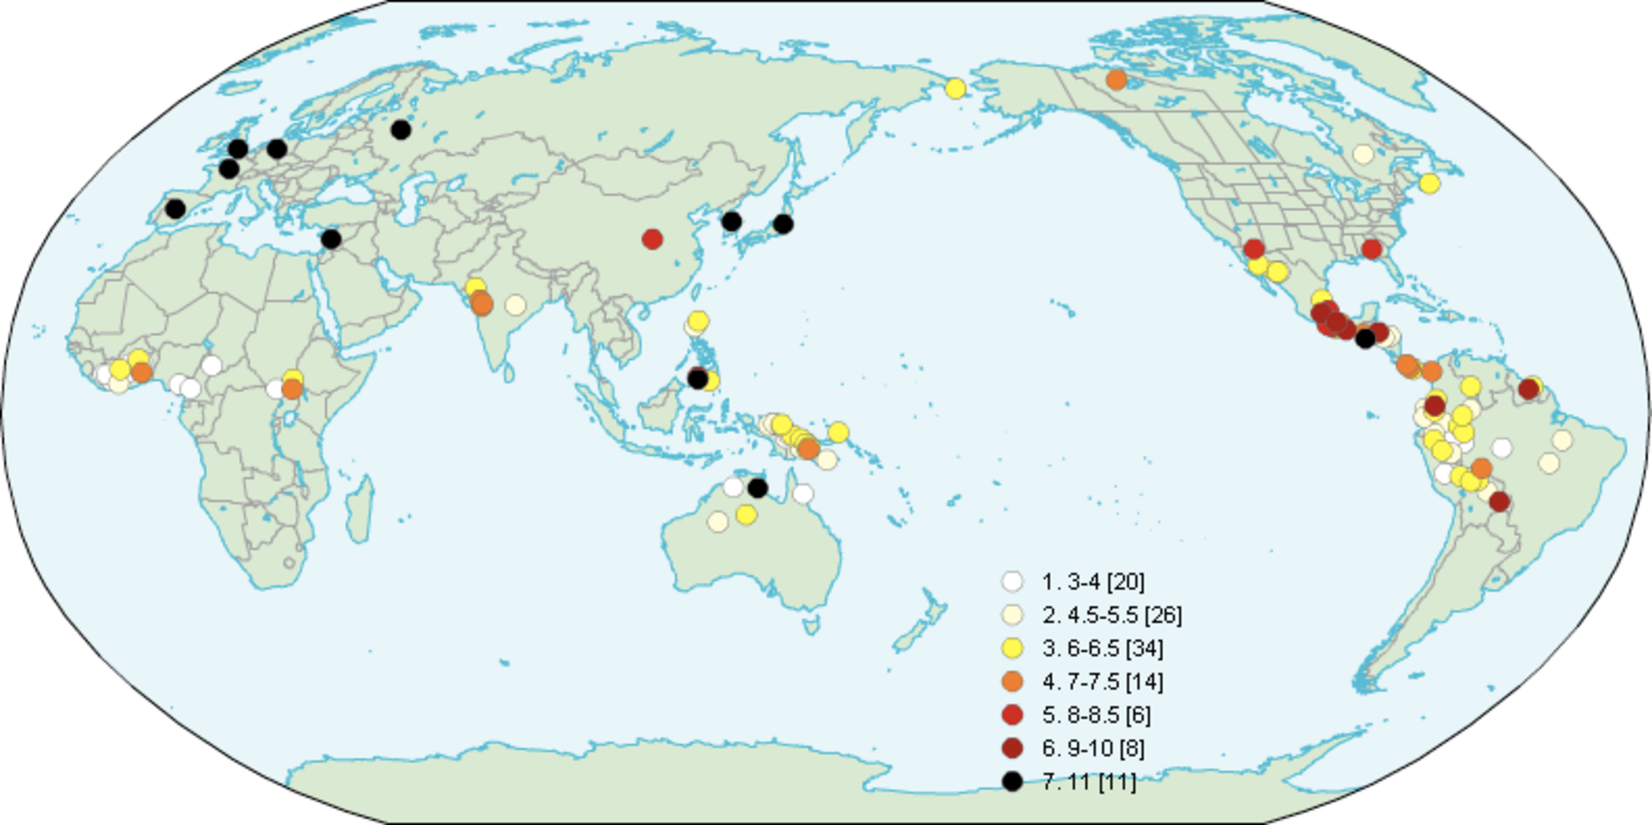
\includegraphics[width=\textwidth]{./intro/figures/number-bcts.pdf}
    \caption[The number of basic colour terms around the world]{The
      number of basic colour terms in languages around the world
      \citep{kay08number}.}
    \label{f:number-bcts}
  \end{center}
\end{figure}

Other systems based on this strategy vary in which dimensions of the
colour domain are relevant for the basic colour terms. The basic
colour system of Hunan\'oo, a language spoken by the Mangyans in the
Philippines, consists of four colour terms: \textit{(ma)biru} (blackness),
\textit{(ma)lagti} (whiteness), \textit{(ma)rara} (redness) and \textit{(ma)latuy}
(greenness). In this system only the lightness and the red-green
opponent channel are relevant to name colours whereas the yellow-blue
opponent channel is ignored \citep{conklin55hanunoo}.

\subsection{Graded membership strategy}

The fact that each colour category has a focal colour also
implies that other colour samples are worse examples of a particular
colour category. Some languages allow their users to mark how well a
particular sample represents the prototype. In English this marking is
optional and achieved through the adverb \textit{very} and the modifying
\textit{-ish} suffix, for instance in the expression \textit{greenish}. In other
languages, such as Tarahumara, which is an indigenous language spoken
in the North of Mexico, this marking is obligatory. This language has
an elaborate system of modifiers that distinguishes three levels of
membership: \textit{-kame} which could be translated as \textit{very}, \textit{-name}
which could be glossed as \textit{somewhat} and \textit{-nanti} for the lowest
degree of membership. An example of how this system is used for the
Turahumara colour category for red: \textit{Sit\'a-''} is shown in Figure
\ref{f:tarahumara} \citep{burgress83tarahumara}.

\begin{figure}[htbp]
  \begin{center}
   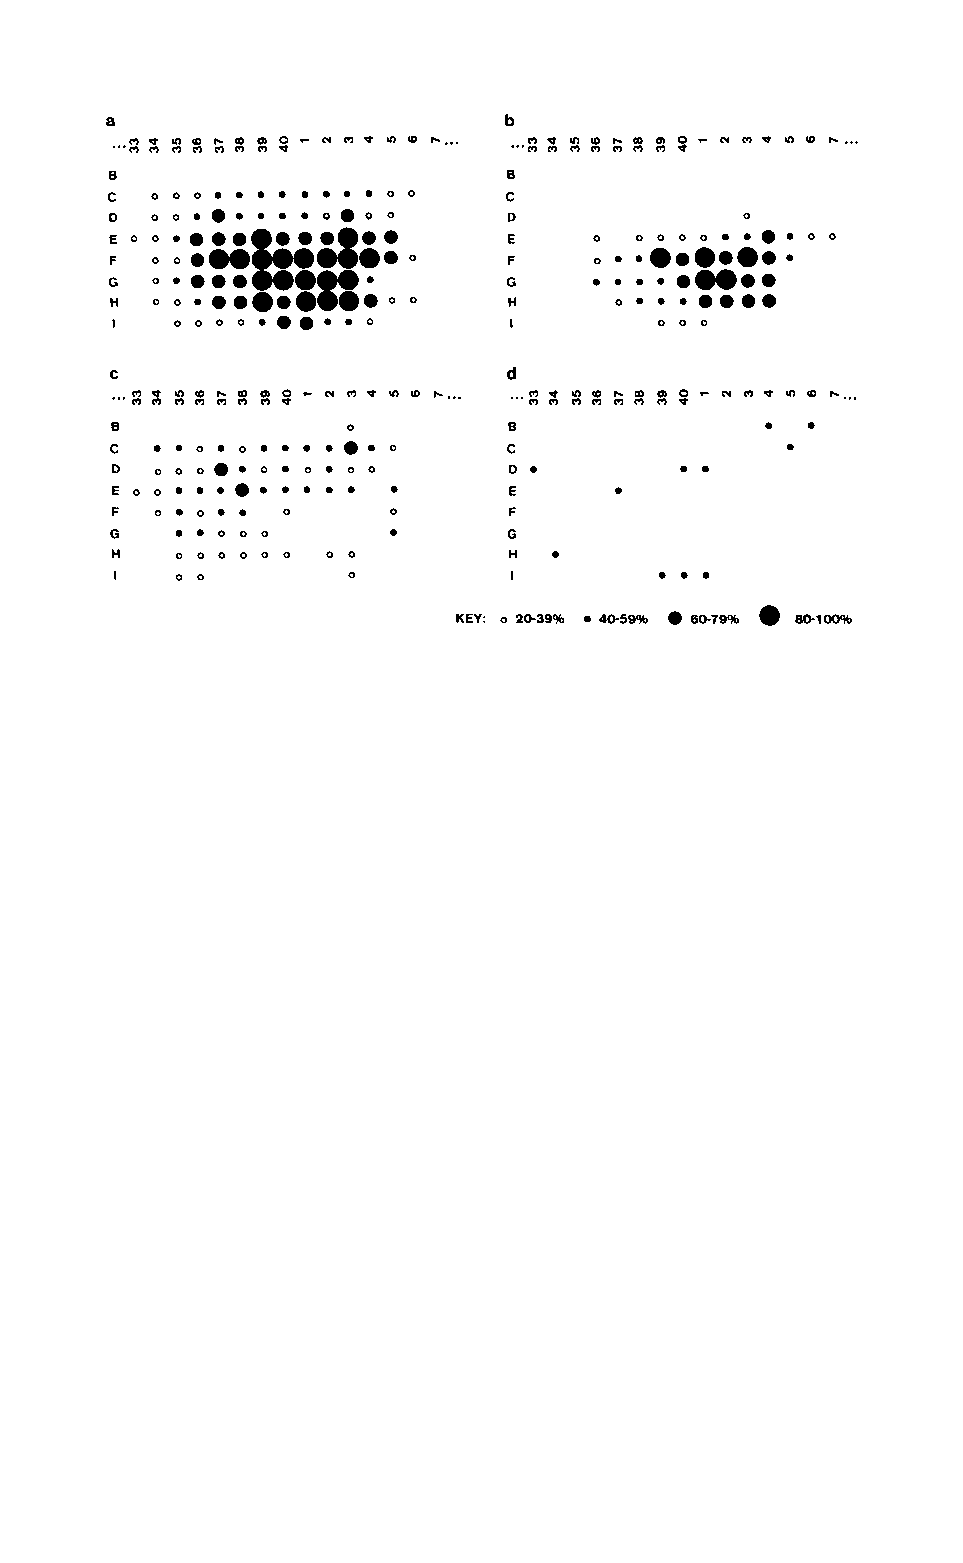
\includegraphics[width=\textwidth]{./intro/figures/tarahumara.pdf}
   \caption[The use of modifiers in Tarahumara]{The use of modifiers
     to express graded membership in Tarahumara shown on an array of
     Munsell chips. The bigger the circle, the more it represents a
     particular colour expression. (a) aggregate of all expressions
     using the \textit{Sit\'a} root (b) \textit{Sit\'akame} (very red) (c)
     \textit{Sit\'aname} (somewhat red) (d) \textit{Sit\'ananti} (only slightly
     red). Note how each modifier specifies a region that is further
     removed from the prototypical colour of \textit{Sit\'a}. Figure from
     \cite{burgress83tarahumara}.}
    \label{f:tarahumara}
  \end{center}
\end{figure}

\subsection{Compounding strategy}

Some languages also allow users to compound two colour categories into
a new one. Especially to describe a colour sample that is not a good
example of any of the basic colour categories, this might be a very
productive strategy that increases expressivity. An example in English
would be ``blue-green''. This compounding can also be modulated by
additional markers, like for example the ``-ish'' marker as in
``brownish-red'' in English.

\cite{safuanova07russian} have collected data on the focal colours of
compounds in Russian. One of their main findings is that in Russian
the order in which colour terms are compounded has an influence on
the resulting focal colour: the second term seems to be more important
in the expression. This is illustrated in the upper left segment of
Figure \ref{f:category-combination}. The colours between ``\v
z\"eltyj'' (yellow) and ``zel\"enyj'' (green) are for example named:
``zelenovato-\v z\"eltyj'' (greenish-yellow), ``zel\"eno-\v z\"eltyj''
(green-yellow), ``\v z\"elto-zel\"enyj'' (yellow-green) and ``\v
z\"eltovato-zel\"enyj'' (yellowish-green) where the suffix ``-ato''
acts as a modulator.

\begin{figure}[htbp]
  \begin{center}
   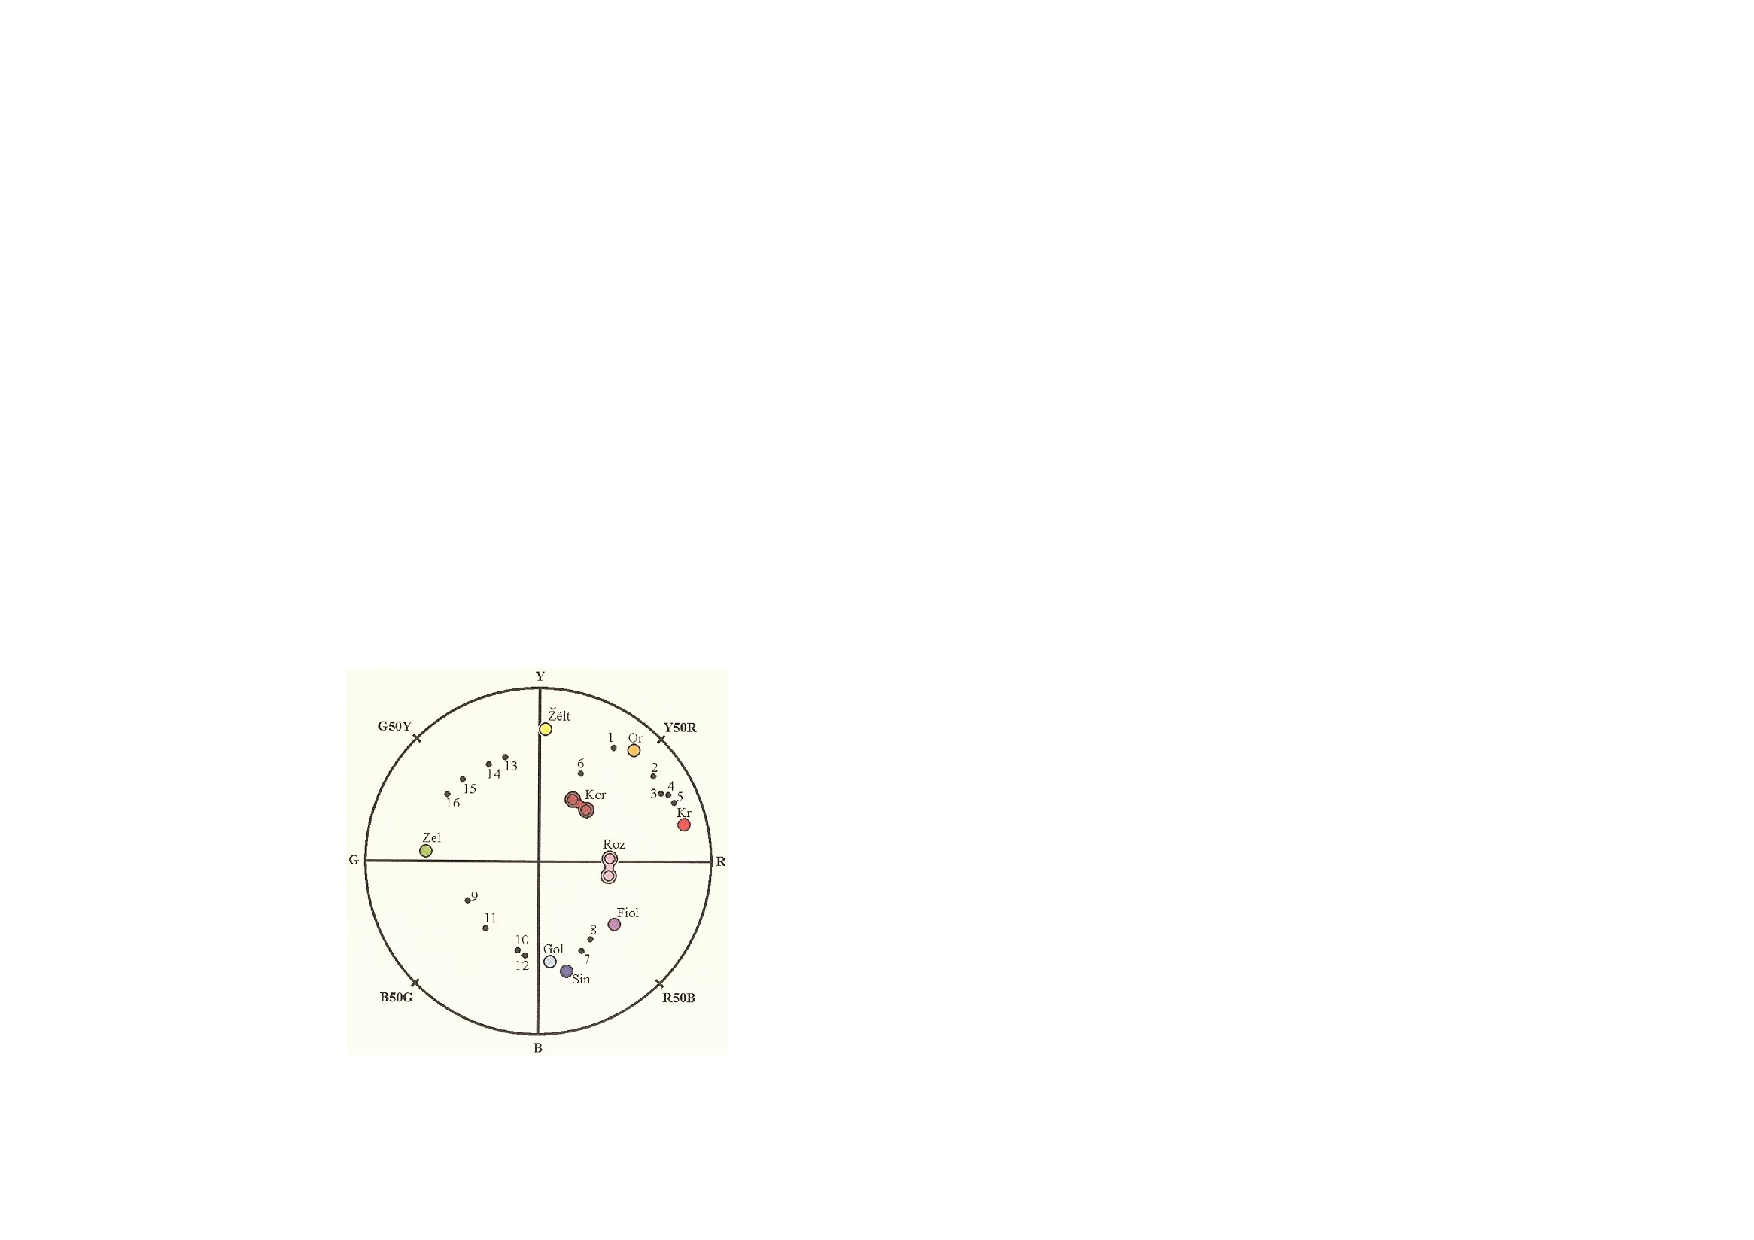
\includegraphics[width=0.6\textwidth]{./intro/figures/category-combination.pdf}
   \caption[Compound chromatic terms in Russian]{Compound chromatic
     terms projected on the hue plane of the NCS colour space. The
     second term in the compound clearly has a bigger impact on the
     resulting focal colour than the first one. The colours between
     ``\v z\"eltyj'' (yellow) and ``zel\"eno" (green) are for example
     named: (13) ``zelenovato-\v z\"eltyj'' (greenish-yellow), (14)
     ``zel\"eno-\v z\"eltyj'' (green-yellow), (15) ``\v
     z\"elto-zel\"enyj'' (yellow-green) and (16) ``\v
     z\"eltovato-zel\"enyj'' (yellowish-green). Figure from
     \cite{safuanova07russian}.}
    \label{f:category-combination}
  \end{center}
\end{figure}

\subsection{Basic modification strategy}

Similarly, many language systems allow for the use of basic
modifiers which modify some aspects of a colour category. In English
for example, users can modify the brightness and the chromaticity of a
colour category through the use of modifiers (``light'' or ``dark''
for modifying the brightness and ``bright'' or ``pale'' for modifying
the chromaticity). This strategy has been attested for a wide range of
languages, including Vietnamese \citep{alvarado02modifying} and
Chinese \citep{lin01unconstrained}.

Although basic modifiers are quite commonly used, only a few
papers report on the exact transformation that is implied by these
modifiers. One exception is the study by \cite{safuanova07russian} of
the Russian language, in which the authors determined the focal
colours of the modified categories. An example of such an analysis in
the Natural Color Sytem (see Appendix \ref{s:NCS}) is shown in Figure
\ref{f:intro-russian-modifiers}. The modifiers ``t\"emno-'' (dark) and
``svleto'' (light), modify the focus of the basic category parallel to
the blackness dimension (W-S). The modifiers ``bledno-'' (pale) and
``jarko-'' (bright) shift the chromaticity of the basic colour
category (W-C or S-C) \citep{safuanova07russian}.

\begin{figure}[htpb]
  \centering
  \includegraphics[width=.6\textwidth]{./intro/figures/russian-diagram.pdf}
  \caption[Location of modified basic colour foci in Russian]{Location
    of modified basic colour foci in Russian projected into the NCS
    blackness-chromaticity triangle. ``t\"emno-'' \emph{dark} (solid
    circle), ``jarko-'' \emph{bright} (sun), ``svetlo-'' \emph{light}
    (open circle) and ``bledno-'' \emph{pale} (dashed circle). Figure
    from \cite{paramei05singing}.}
  \label{f:intro-russian-modifiers}
\end{figure}

\subsection{Other strategies}

Another strategy that is often used to name colours, is suggesting
colours by naming an object that is typical for that colour (like for
example ``lavender'' or ``salmon'' in English). These object names can
also be used in combination with basic colour terms (like ``sky blue''
or ``cherry red''). Even though the abundant usage of these terms has
been confirmed in unconstrained naming experiments, like for example
in English and Chinese \citep{lin01unconstrained}, the actual focal
colours of these expressions have yet to be determined. The previous
list of language strategies is not exhaustive, as other strategies to
describe colours exist (for example using comparatives like in ``most
green'').

\section{Modelling a language strategy}
\is{language strategy!modelling}

Modelling a language strategy starts with the reverse engineering of
the semantic and syntactic templates that allows language users to
conceptualise and express a particular subarea of meaning in
language. A language strategy also includes the operationalisation of
a series of learning operators, which will be discussed later.

In the \emph{basic colour strategy}, the semantic template defines how
to select the appropriate colour category to describe a colour sample,
for example, the category that is most similar to that sample. The
syntactic template could then define a lexicon in which categories are
associated to terms. These templates can be used in both production
and interpretation.

The performance of the semantic and syntactic templates can be
evaluated in a \emph{baseline experiment}\is{baseline experiment}. 
In such an experiment, these templates are instantiated
based on a natural language system that is provided by the
experimenter. It allows to model a natural language system and to test
its simulated performance in a benchmark using simulated language
users, or agents.

\subsection{Modelling linguistic interaction}
\label{s:intro-language-games}

In order to model the function of a language strategy, I will use the
language game paradigm \citep{steels96self}. In this paradigm,
language users are modelled as \emph{agents}\is{agent} and a language community
as a \emph{population of agents}. These agents constantly engage in
local interactions, or \emph{language games}\is{language game} in
which they try to achieve \emph{communicative
  goals}\is{communicative goal}, like for example drawing the
attention of another agent to one of the objects in a shared
environment or \emph{context}\is{context}. Achieving these communicative goals is considered to be
the function of a language strategy.

A language game typically involves two agents randomly drawn from the
population. One is assigned the role of the speaker and the other the
role of the hearer. The speaker selects a private communicative goal,
for which it conceptualises a meaning. Using its current linguistic
knowledge it produces an utterance to express this meaning. The hearer
parses this utterance using its own current linguistic knowledge and
interprets the resulting meaning in his own world model. This
interpretation might lead to some actions which should allow the
speaker to verify whether the intended communicative goal was
reached. If this is not the case, the speaker reveals the
communicative goal to the hearer. Both agents update their linguistic
and conceptual knowledge in order to become more successful in future
interactions. All the processes involved in one interaction are
summarised in a \emph{semiotic cycle}\is{semiotic cycle} which is
shown in Figure \ref{f:intro-semiotic-cycle}
\citep{steels03reentrance}.

\begin{figure}[htbp]
  \begin{center}
   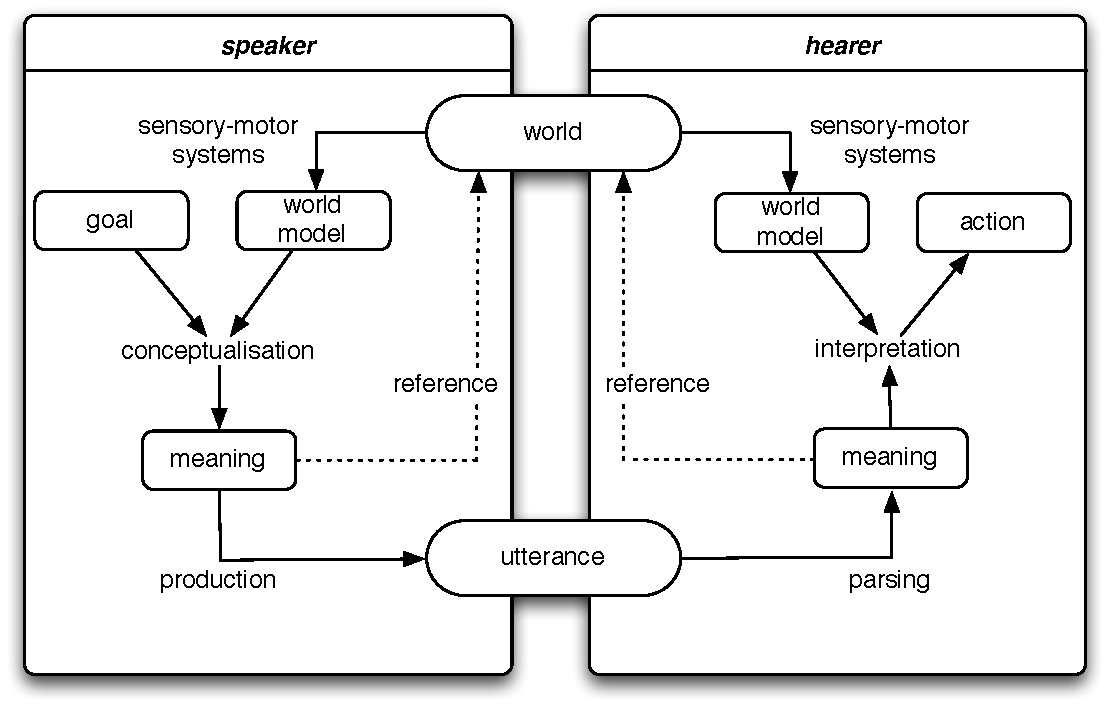
\includegraphics[width=\textwidth]{./intro/figures/semiotic-cycle.pdf}
   \caption[The semiotic cycle of a language game]{The semiotic cycle
     of a language game. The speaker selects a communicative goal
     using its own world model, conceptualises a meaning and renders
     an utterance for this meaning. The hearer parses this utterance
     into meaning which is interpreted using its own world model. This
     interpretation might lead to some action, upon which the speaker
     provides feedback (not shown in figure).}
    \label{f:intro-semiotic-cycle}
  \end{center}
\end{figure}

\subsubsection{Language games for colour}
\label{s:language-games-for-colour}

The first language game in which colour could be expressed by the
agents, was the Talking Heads experiment
\citep{steels99talking}. In this experiment contexts consisted
of coloured geometrical figures on a whiteboard which were perceived
by two pan-tilt cameras. Software agents could be embodied in these
cameras. The communicative goal was to draw the attention of the other
agent to one of these figures.The agents could describe several
domains to achieve this goal, including the domain of colour. It soon
became apparent that the domain of colour was rich and complex enough
to be studied in isolation.

This observation led to the development of the \emph{Colour Naming
  Game}\is{language game!Colour Naming Game}\is{Colour Naming
  Game|see{language game}} \citep{steels05coordinating,
  belpaeme05explaining, belpaeme07language, puglisi08cultural,
  baronchelli10modeling} in which agents were restricted to use only
the domain of colour to achieve the communicative goal. The use of
information in other domains, for example spatial relations, was not
allowed. The Colour Naming Game has been devised to study how a
population of agents can form and align its own colour category
systems. In these studies the contexts were based on the random
selection of a number of colour samples from a large set of
colour samples. A colour sample is an abstract representation that
only contains colour information.

In the \emph{Grounded Colour Naming Game}\is{language
game!Grounded Colour Naming Game}\is{Grounded Colour Naming
Game|see{language game}} (see Section \ref{s:experiments-grounded}),
embodied agents (robots) are placed in a closed office environment and
the contexts consisted of toy-like objects that are placed in front of
the agents. Although embodied agents could easily use different
domains to describe the objects in front of them, they are only
allowed to describe the colour information of these objects. In this
language game, the utterances are still restricted to a single term.

I introduce the \emph{Colour Description Game}\is{language
  game!Colour Description Game}\is{Colour Description
  Game|see{language game}} (see Chapters
\ref{s:graded-membership-strategy}-\ref{s:basic-modification-strategy})
in which the restriction of using a single colour term to describe the
colour of an object is lifted.

\subsubsection{Background assumptions}

The language paradigm focusses on the functional and evolutionary
aspect of languages, but this can only be achieved by making some
assumptions. It is assumed that agents are capable of giving joint
attention \citep{tomasello95jointattention}, constructing world
models, taking turns, being cooperative\footnote{\cite{wang08self}
  show that uncooperative agents can also bootstrap a language under
  certain conditions}, and so on. These assumptions are each
interesting and far from trivial research topics by
themselves. Although it is clear that these processes are
prerequisites for studies in the language game paradigm, they are not
in the main focus of this paradigm.

\section{Self-organisation of language systems}

A language system is not a static system, but rather a living system
that is constantly evolving. In the self-organisation of language systems
based on the basic colour strategy, language systems are expanded by
the introduction of new colour categories. By studying a wide range of
contemporary language systems for colour, some researchers have even
proposed a universal evolutionary order by which colour categories are
introduced to a language \citep{berlin69basic}.

% todo: meer uitleg

\section{Modelling the self-organisation of language systems}

In order to model the self-organisation of language systems\is{language system!self-organisation of}, 
the implementation of a language strategy needs
to be extended with a series of learning operators that specify:

\begin{enumerate}
\item how a language user can acquire a language system from other
  language users using \emph{adoption operators}\is{learning operators!adoption operator}
\item how language users can update their knowledge of the language
  system after a linguistic interaction using \emph{alignment
    operators}\is{learning operators!alignment operator}
\item how a language user can expand a language system using
  \emph{invention operators}\is{learning operators!invention operator}
\end{enumerate}

For the basic colour strategy, the adoption operator allows a user to
adopt a new colour category and its associated colour term when a new
unknown term is encountered. The invention operators allow users to
introduce new colour terms that are associated to new colour
categories to the language system. Finally, the alignment operator
specifies that agents should update their colour categories to better
represent the topic when the linguistic interaction was successful.

An \emph{acquisition experiment}\is{acquisition experiment} could be implemented in which the
adoption and alignment operators of a language strategy are
tested. Such an experiment involves two agents in which one needs to
acquire a predefined language system from another agent. By comparing
the performance of the agent that is acquiring the language system to
the performance in the baseline experiment, the performance of the
adoption and alignment operators can be evaluated.

The final step would be a \emph{formation experiment}\is{formation experiment} in which a
population of agents needs to construct its own language system from
scratch. Such an experiment checks the performance of the invention
operators by comparing the performance of the population of agents in
this experiment to the baseline performance.

\subsubsection*{Language as a complex adaptive system}
 
Within the language game paradigm, a language system is considered to
be a complex adaptive system \citep{steels00language}. It is shaped
and reshaped by its users to suit their needs, even over the course of
a single dialogue \citep{garrod94conversation}, in order to become
more successful in communication while minimising cognitive effort. No
single user has a complete view of the language and no user can
control the linguistic behaviour of the complete group. Instead,
language is a self-organising system that emerges through local
interactions or language games.

\section{Evolution of language strategies}
\is{language strategy!evolution}

If one takes a historical perspective on language, one can also
detect shifts in dominance from one language strategy to another. In
the evolution of the basic colour terms in English an interesting
meaning shift occurred: at their Indo-European root most colour terms
had primarily a brightness meaning sense. Around the transition from
Old to Middle English the hue meaning sense of all basic colour terms became
more dominant than the original brightness sense
\citep{casson97shift}. Both meaning senses could be thought of as
different variations of the basic colour strategy.

This is illustrated in Figure \ref{f:history-yellow} in which the
history of the term ``yellow'' is shown. In Indo-European its
syntactic form was ``ghel'' which was primarily used to refer to the
shining (of yellow metals). In Old English the term ``geolo'' acquired
a hue sense and could be used to refer to the colour of some silk
cloth. In the transition to Middle English ``yelou'' the hue sense
became the more dominant one and the term could also be used to refer
to for example yolk and ripe corn, although it could still be used to
refer to gold. The same is true for all other basic colour terms. Most
interestingly all colour terms that were introduced to English after
this shift, like for example ``orange'', never had a brightness sense
but only a hue sense \citep{casson97shift}. Similar meaning shifts
have been reported in a wide range of languages
\citep{maclaury92brightness}.

\begin{figure}[htbp]
  \begin{center}
   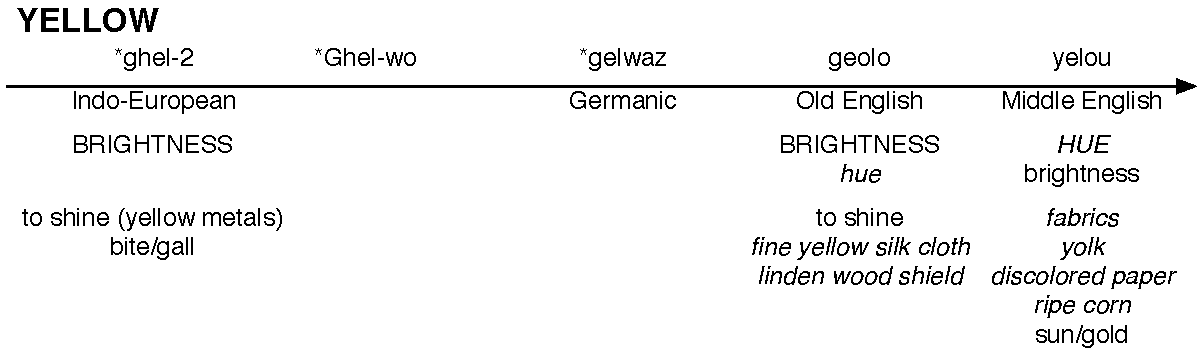
\includegraphics[width=\textwidth]{./intro/figures/history-yellow.pdf}
   \caption[The evolution of the term ``yellow'' in English]{The
     evolution of the term ``yellow'' in English. Like almost all
     other basic colour terms, its meaning shifted from brightness to
     hue around the transition from Old English to Middle
     English \citep{casson97shift}.}
    \label{f:history-yellow}
  \end{center}
\end{figure}

\section{Modelling evolution of language strategies}

Given the observed evolution and selection at both the level of
language strategies and the level of linguistic items that make up a
particular language system, I explore the hypothesis that linguistic
agents need explicit representations of language strategies which they
use to keep track of how successful a particular strategy has been in
communication. These explicit representations allow me to introduce an
additional layer of selection at the level of language strategies.

\section{Structure of this book}

Chapter \ref{s:formalisms} will introduce the formalisms that will be 
used to model language strategies and language systems.

In part \ref{s:language-strats} of this book focusses on the
reconstruction of the general semantic and syntactic structures that
allow me to run baseline experiments for several of the language
strategies identified in this chapter: the basic colour strategy, the
graded membership strategy, the compounding strategy and the
basic modification strategy.

In part \ref{s:evolution-of-language-systems}, I will focus on the
self-organisation of language systems that are based on one language strategy,
namely the basic colour strategy, by introducing its adoption,
alignment and invention operators. This will allow me to study the
impact of embodiment on the performance of these operators. I will
also show results of related experiments on language systems that are
realisations of this strategy.

In part \ref{s:evolution-of-language-strategies} of this book, I
will present a model that allows to study the evolution of language
strategies based on linguistic selection. I will start by introducing
two variants of the basic colour category and show an experiment that
models the meaning shift as documented for the history of basic colour
terms. I will also explore the origins of language strategies based on
a combinatorial search process.

Part \ref{s:conclusion} will conclude this book with an overview of
the main results that have been achieved in this book and will
outline some directions for future research.

\chapter{Formalisms for language systems and language strategies}
\label{s:formalisms}

Modelling a language strategy encompasses defining semantic and
syntactic templates and applying realised templates that make up a
language system. Moreover, the language strategy needs to define
adoption, alignment and invention operators. This imposes hard
requirements on the formalisms that are needed to model a language
strategy.

Standard first-order formalisms in logic that are commonly used in
artificial language evolution research, such as predicate logic, are
insufficient to represent the semantic templates of some of the
strategies outlined in the previous chapter. For example, the meaning
of a realisation of the graded membership strategy, such as \textit{very
red}, cannot be expressed using any first-order logical formalism in
a satisfactory way as the the adverb \textit{very} modifies the meaning of
the adjective \textit{red}.

The syntactic templates require a grammar formalism, as the word order
seems to have an impact on the resulting focal colour that is
intended.  This is for example the case in the compounding strategy in
Russian, where \textit{zel\"eno-\v z\"eltyj} (`green-yellow') is different
from\textit{\v z\"elto-zel\"enyj} (`yellow-green'). This difference implies
that the lexical approach in which the lexicon captures a direct
association between terms and colour category is no longer sufficient.

In this book, I have chosen to use \emph{Incremental Recruitment
  Language} (IRL) to represent semantic templates and \emph{Fluid
  Construction Grammar} (FCG) to represent syntactic templates. Both
formalisms have been especially designed to support experiments in
artificial language evolution \citep{loetzsch09understanding}.

This chapter provides a short introduction to both systems that
introduces the design principles behind these formalisms and that
should enable the reader to understand the models of language
strategies that will be presented in future chapters. Readers can
choose to skip this chapter and return to it when needed.

\section{Embodied cognitive semantics using IRL}
\label{s:irl}
\is{Incremental Recruitment Language|see{IRL}}
\is{IRL}

\subsection{Theoretical foundations}

Although research on the emergence of communication systems with
similar features as human natural language has shown important
progress, the complexity of the meanings considered so far remains
limited. Experiments either use simple categories
\citep{steels05coordinating, belpaeme05explaining}, conjunctive
combinations of categories \citep{wellens08flexible} or
predicate-argument expressions \citep{batali02negotiation,
  smith03iterated, debeule08emergence}. Natural languages are clearly
capable of expressing second order semantics
\citep{dowty1981introduction}. For example, the adverb \textit{very} in
\textit{very big} modifies the meaning of the adjective, it is not just a
simple conjunction of the predicates \textit{very} and \textit{big}. Moreover the
same predicate (e.g. \textit{big}) can often be used in different ways, for
example to further restrict the set of possible referents of a noun
(as in \textit{the big ball}), to state a property of an object (as in
\textit{the ball is big}), to reify the predicate itself and make a
statement about it (as in \textit{big says something about size}), to
compare the elements of a set (as in \textit{this ball is bigger than the
others}), etc. The specific usage of a predicate in a particular
utterance is clearly conveyed by the grammar, so any theory on the
origins and evolution of grammar must address second order semantics.

The semantics of the utterances in this book are not represented in
a standard logic, but in an alternative framework, Incremental
Recruitment Language or IRL \citep{steels00emergence,
  steels05planning, vandenbroeck07constraintbased,
  vandenbroeck08constraintbased}. In this framework the meaning of a
sentence is a \emph{semantic constraint network} that the speaker
wants the hearer to evaluate in order to achieve the communicative
goal selected by the speaker. This approach resonates with earlier
work in AI on procedural semantics \citep{winograd72understanding}.

The IRL framework has been especially designed for experiments on
artificial language evolution and therefore supports key features that
have been proven successful in this field of research. It is
\emph{omni-directional}: not only can it be used for both
conceptualisation and interpretation but also to complete partial
semantic constraint networks. This feature does not only enable both
speaker and hearer to use the same formalism, but it has also proven
to be crucial when writing adoption, alignment and invention
operators. The speaker can use it to diagnose potential problems in
communication by interpreting its own utterance to detect potential
ambiguities \citep{steels03reentrance}. The hearer can try to
reproduce a partially understood meaning together with the
communicative goal, revealed by the speaker in a failed interaction,
to infer which parts it misinterpreted or did not know yet. On a
technical level, this strongly suggests a constraint-propagation
language \citep{marriott98programming}.

Another key feature of IRL is its \emph{open-endedness} towards the
cognitive operations it can represent. Previous research has deployed
a wide range of such operations including discrimination trees
\citep{steels96perceptually}, event feature detectors
\citep{siskind01grounding}, nearest neighbour classification
\citep{belpaeme05explaining} and radial basis function networks
\citep{steels05coordinating}.  IRL aims to be an overarching formalism
which can support any cognitive operation for which a tractable
implementation on a computer exists. It can be used for rich semantics
in which any of these operations can be combined and also for
experiments in which the choice of the cognitive operation is not
predetermined by the experimenter.

Finally, IRL is designed to support world models which are
\emph{grounded} in the sensory-motor system of the agent. These world
models are non-symbolic and are based on the operation of their
sensori-motor apparatus. Often \citep[e.g.][]{batali02negotiation,
  smith03iterated, wellens08flexible} it is assumed that there is a
simple straightforward mapping of the non-symbolic world model onto a
categorial situation model, which is a representation of the world in
the form of facts in some variant of predicate calculus. But as
different languages conceptualise the world in different ways, this
mapping function is clearly nontrivial.

\subsection{Semantic constraint network}
\label{s:semantic-constraint-network}
\is{semantic constraint network}
\is{semantic network|see{semantic constraint network}}

The meaning of an utterance will be viewed as a \textsc{semantic
  constraint network}, or \textsc{semantic network} for short. The basic
nodes of these networks are \textsc{primitive
  constraints}\is{primitive constraint} which reflect cognitive
operations and which are provided by the experimenter.  Each
constraint has a number of arguments which can be bound to a certain
variable. Variables are denoted using a question mark prefix. If a
variable appears as an argument to more than one constraint, it means
the value for this variable is constrained by more than one
constraint. Some variables can be bound to a certain \textsc{semantic
  entity}\is{semantic entity} by means of a bind
statement. Semantic entities are marked by square brackets.

An example network for an utterance like \textit{the block} is shown in
Figure \ref{f:context-and-network} to identify the block within a
hypothetical context. The {\sc Equal-to-Context} primitive (primitives
will always be printed in small capitals) binds all entities in the
context to $?s1$. The {\sc Filter-Set-Proto\-type} primitive takes
this entity-set as input, computes all entities that are similar to
the prototype of a block (provided by the bind statement through $?p1$)
and binds the resulting set to $?s2$. Finally, the {\sc
  Select-Element}, of which the selector is specified as [unique],
checks whether this set contains only one element and binds this
element to $?t$.

\begin{figure}
\centering
\subfigure[]{
  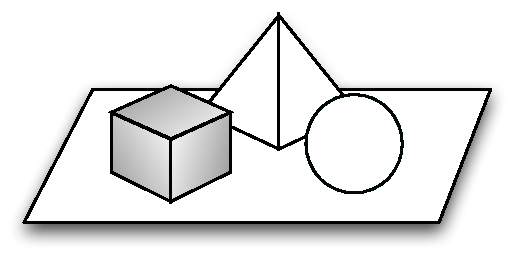
\includegraphics[width=0.45\textwidth]{./frameworks/figures/context.pdf}
  \label{f:context}
}
\subfigure[]{
  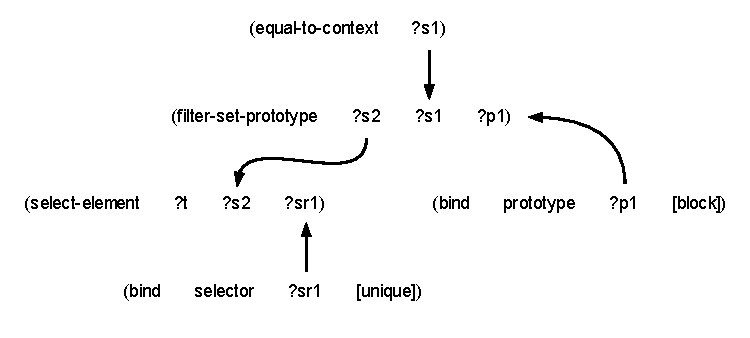
\includegraphics[width=\textwidth]{./frameworks/figures/network.pdf}
  \label{f:network}
}
\caption[Example semantic constraint network for \textit{the block}]{\subref{f:context} a hypothetical context \subref{f:network}
  an example of a semantic constraint network for \textit{the block} to
  identify the topic within (a) (marked in grey for clarity)}
\label{f:context-and-network}
\end{figure}

The more complex the world (for example by adding a second block), the
more complex the semantic constraint network will need to be in order
to achieve this goal (for example extending the previous one with
another filter operation based on size). An example of such a context
and such a network is shown in Figure
\ref{f:more-complex-context-and-network}. This network could represent
the meaning of an utterance like \textit{the big block}. The entity-set of
all blocks in $?s2$ is now further filtered to contain only big blocks
using the {\sc Filter-Set-Category} primitive, which binds the
resulting set to $?s3$ which is passed on to the {\sc Select-Element}
primitive. Note that the previous network in Figure \ref{f:network}
would fail in this context as the {\sc Select-Element} primitive with
a [unique] selector constrains the number of blocks in the context to
be one at most.

\begin{figure}[htbp]
\centering
\subfigure[]{
    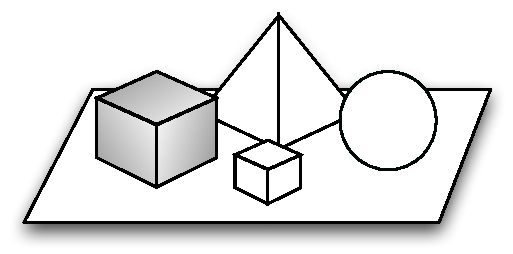
\includegraphics[width=.45\textwidth]{./frameworks/figures/more-complex-context.pdf}
  \label{f:more-complex-context}
}
\subfigure[]{
    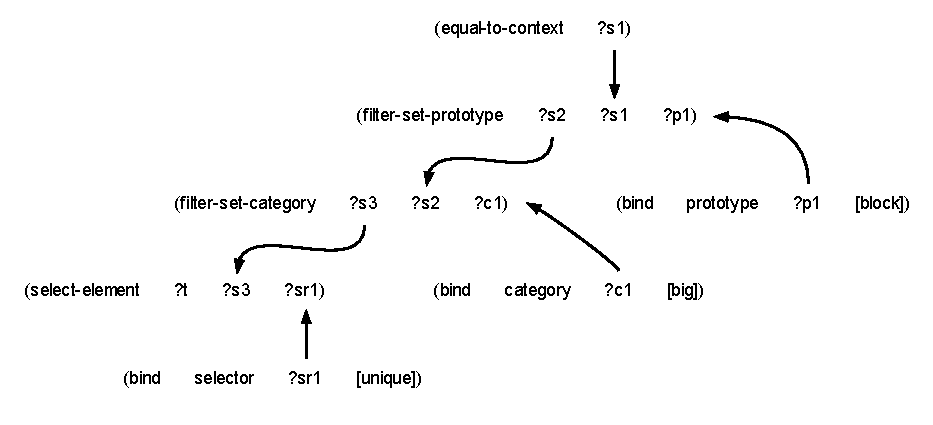
\includegraphics[width=\textwidth]{./frameworks/figures/more-complex-network.pdf}
  \label{f:more-complex-network}
}
\caption[Example semantic constraint network for \textit{the big
block}]{\subref{f:more-complex-context} a more complex hypothetical
  world \subref{f:more-complex-network} a more complex semantic
  constraint network to identify \textit{the big block} (marked in grey for
  clarity)}
\label{f:more-complex-context-and-network}
\end{figure}

\subsection{Evaluation}
\is{semantic constraint network!evaluation}

The evaluation of a semantic constraint network involves cycling
through the primitives of the network until each primitive has been
successfully revised. The revision of a primitive has three possible
outcomes: (1) validation with possible bindings for one or more of its
arguments (2) rejection or (3) suspension. Whenever a primitive
returns more than one possible solution, the evaluation tree which
keeps tracks of possible bindings for each variable in the network,
splits. This especially occurs during conceptualisation when the
semantic entities of the primitive constraints are still
unknown. Whenever a primitive rejects a particular set of bindings,
that particular branch in the evaluation tree can not be explored any
further. Whenever a primitive is not specified for a certain pattern
of bound or open arguments, it is suspended and revised at a later
moment.

During conceptualisation, the topic is typically known but the
semantic entities of the cognitive operators (like for example which
prototype or which category to use) are not. During interpretation,
the opposite is true: the semantic entities of the cognitive operators
have been passed on in the utterance, but the topic has not. A typical
network during interpretation is shown in Figure
\ref{f:more-complex-network}. The same network during
conceptualisation is shown in Figure
\ref{f:network-conceptualisation}.

The evaluation process of this network is shown in Figure
\ref{f:evaluation-process}. The context consists of four objects: a
big block (b-bk), a small block (s-bk), a ball (bl) and a pyramid (pd)
and the goal is to identify the big block in this context, so we have
a binding for $?t$. The only primitive that can be revised is {\sc
  Equal-to-Context} which can bind $?s1$ to the context: \{b-bk, s-bk,
bl, pd\}. The next primitive that can be revised is {\sc
  Filter-Set-Prototype} and let us suppose it knows the prototypes for
block and ball. This will cause a split in the evaluation tree: one in
which $?p1$ is bound to [block] and $?s2$ is bound to \{b-bk, s-bk\}
(node 2) and another branch in which $?p1$ is bound to [ball] and
$?s2$ is bound to \{bl\} (node 3). The next primitive that can be
revised is {\sc Filter-Set-Category}. Let us suppose this primitive is
only defined when its second argument contains at least two
entities. This will lead to a rejection of the branch of node 3 and to
a further split of the branch of node 2: one in which $?c1$ is bound
to [small] and $?s3$ is bound to \{s-bk\} (node 4) and another branch
in which $?c1$ is bound to [big] and $?s4$ is bound to \{b-bk\} (node
5). The final primitive that needs to be revised is {\sc
  Select-Element}, which checks whether $?s4$ contains only one entity
that is equal to the big block. This leads to a rejection of the
branch of node 4 but also to a successful evaluation of the branch of
node 5 in which $?sr1$ is bound to [unique].

\begin{figure}[htbp]
\centering
\subfigure[]{
    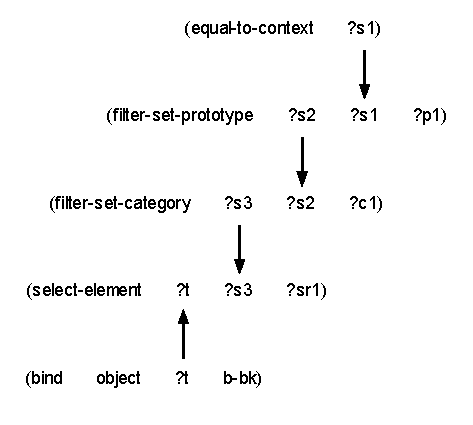
\includegraphics[width=.60\textwidth]{./frameworks/figures/network-conceptualisation.pdf}
  \label{f:network-conceptualisation}
}
\subfigure[]{
    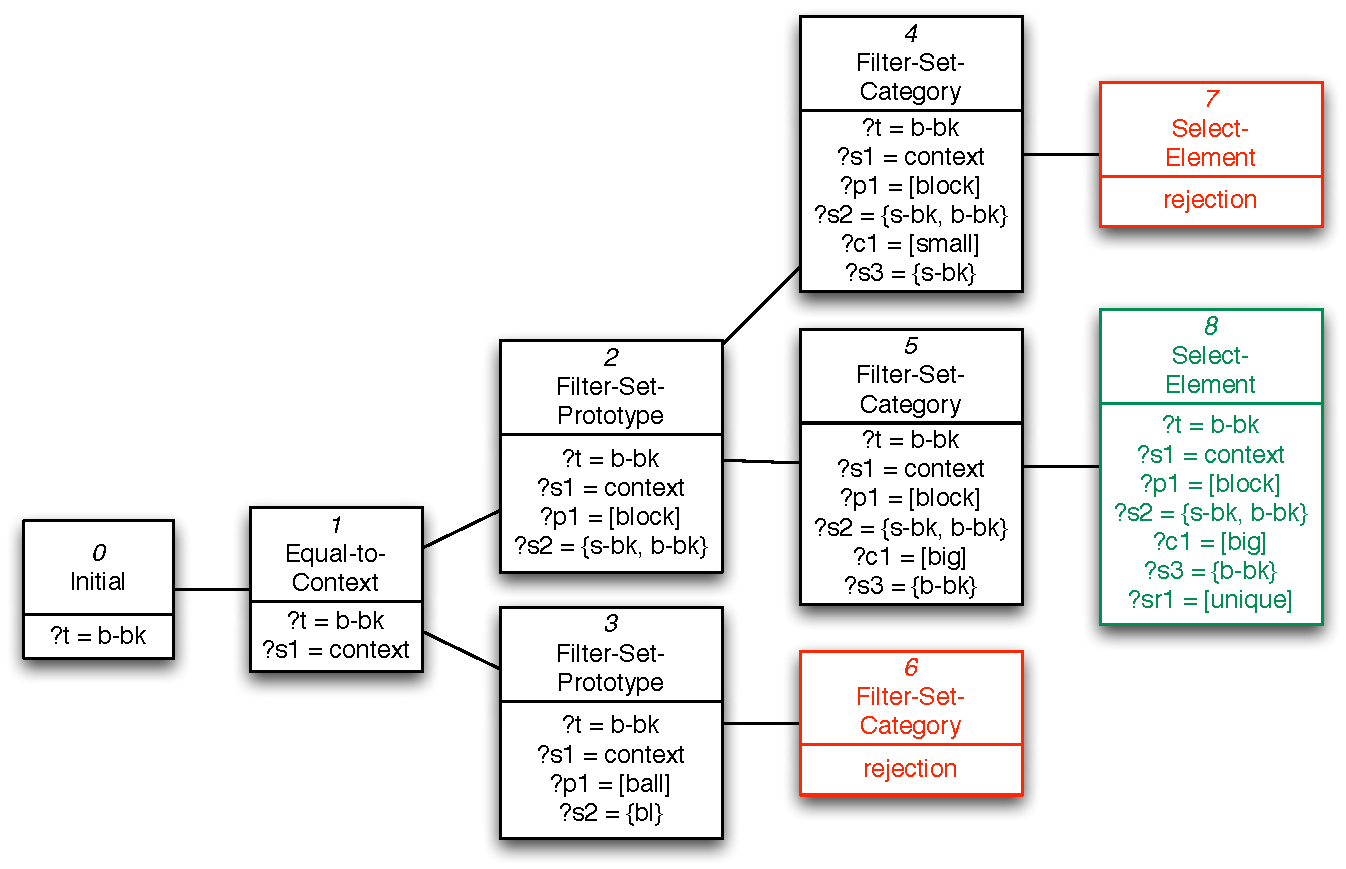
\includegraphics[width=.8\textwidth]{./frameworks/figures/evaluation.pdf}
  \label{f:evaluation-process}
}
\caption[Evaluation process of an example constraint
network]{\subref{f:evaluation-process} The evaluation process of an
  example network \subref{f:network-conceptualisation} during
  conceptualisation in a context consisting of four objects: a big
  block (b-bk), a small block (s-bk), a ball (bl) and a pyramid
  (pd). The communicative goal is to identify the big block.}
\label{f:evaluation}
\end{figure}

During acquisition of new semantic entities, the hearer will have been
able to reconstruct the intended semantic constraint network for a
large part. This network will be extended by the communicative goal
that is revealed by the speaker and will be revised in order to
acquire the semantic entity that fulfills the need in the current
network.

An example of such a network is shown in Figure
\ref{f:network-learning}, which could have been parsed after hearing a
sentence like \textit{the wabado ball}. Due to the omni-directional\-ity of
IRL, the first two arguments of the {\sc Filter-Set-Category}
primitive, $?s3$ and $?s2$ can be completely determined, which allows
IRL to come up with either a category that is already known or with an
entirely new category that would perform the correct filtering.

\begin{figure}[htbp]
  \begin{center}
    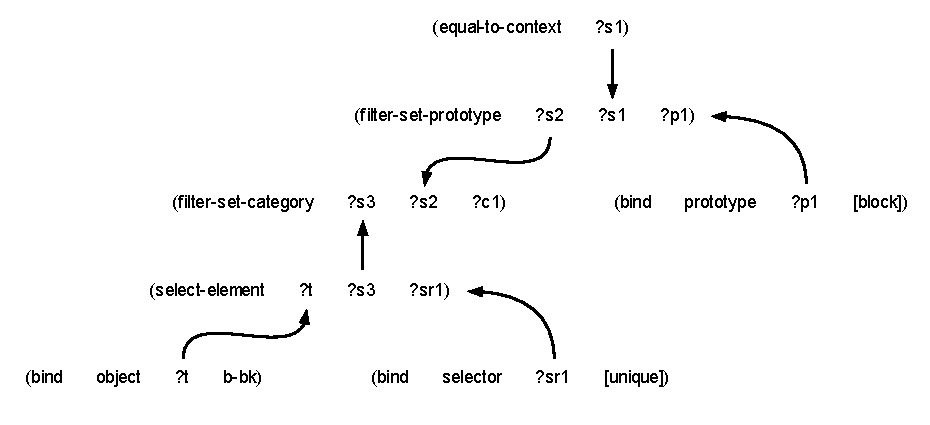
\includegraphics[width=\textwidth]{./frameworks/figures/network-learning.pdf}
    \caption[Example constraint network during learning]{A partial
      network that could be reconstructed by combining information
      from parsing \textit{the wabado ball} and the communicative goal
      revealed by the speaker. Due to the omni-directionality of IRL,
      the first two arguments of the {\sc Filter-Set-Category}
      primitive are sufficient to allow IRL to deduce a valid category
      for $?c1$.}
    \label{f:network-learning}
  \end{center}
\end{figure}

\subsection{Conceptualisation}
\label{s:irl-conceptualisation}
\is{conceptualisation}
\is{semantic constraint network!generation}

Conceptualisation can now be viewed as a search process in which a
semantic constraint network that is suitable to achieve the
communicative goal it selected \citep{steels05planning} needs be
constructed. Agents start with a library of primitive
constraints. These primitives are combined using heuristics to
construct networks that become more and more complex. In general,
these heuristics exploit the typical structure of the arguments of a
primitive and the type information of these arguments. The typical
structure is that the first argument is the target variable which can
be computed based on the values of the other arguments. Type
information is used to ensure that arguments that are linked are of
compatible type. More elaborate heuristics, which for example avoid
duplicate primitive constraints in one network, are also available.

An example of such a search process to identify a single object is
shown in Figure \ref{f:conceptualisation} which starts from a library
of four primitive constraints: {\sc Equal-to-Context}, {\sc
  Filter-Set-Prototype}, {\sc Filter-Set-Category} and {\sc
  Select-Element}. The search process starts from a variable bound to
the topic. This variable is considered to be an open variable for
which a primitive with a compatible target argument needs to be
found. Only one primitive in the library fulfils this requirement:
{\sc Select-Element}. This primitive again introduces an open variable
for its second argument which is of type entity-set. In the next
expansion step of the search tree, three primitives are considered:
{\sc Equal-to-Context}, {\sc Filter-Set-Prototype} and {\sc
  Filter-Set-Category} (nodes 2--4). Node 2 already contains a complete
network and can be evaluated. If the context contains only one object
this network succeeds and the conceptualisation process terminates. If
this is not the case, nodes 3 and 4 will be further expanded as they
again have an open variable of type entity-set. Both nodes can be
expanded with the three primitive constraints that have a compatible
target argument (nodes 5--10). If the topic can be identified using a
single {\sc Filter-Set-Prototype} (node 5) or {\sc
  Filter-Set-Category} (node 8), conceptualisation has been
completed. If not, the search process continues.

\begin{figure}
  \begin{center}
    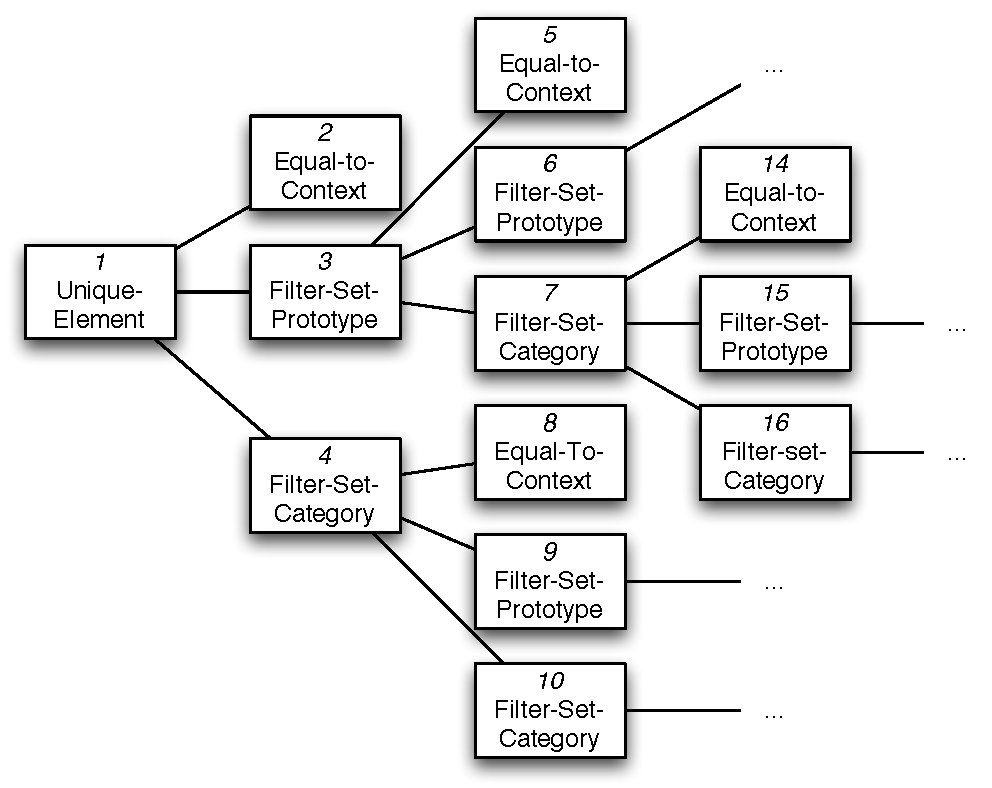
\includegraphics[width=.75\textwidth]{./frameworks/figures/conceptualisation.pdf}
    \caption[Example of the conceptualisation process]{Example search
      tree during conceptualisation, starting from a library of four
      primitives: {\sc Equal-to-Context}, {\sc Filter-Set-Prototype},
      {\sc Filter-Set-Category} and {\sc Select-Element}. The number
      in each node of this tree reflects the order in which they are
      expanding, following a standard breadth-first heuristic. Node 5
      corresponds to the network shown in Figure \ref{f:network}, node
      14 to the one in Figure \ref{f:more-complex-network}.}
    \label{f:conceptualisation}
  \end{center}
\end{figure}

\subsubsection{Chunking}
\label{s:irl-chunking}
\is{IRL!chunking}
\is{chunking|see{IRL}}

Earlier research on automatic programming in knowledge systems
\citep[see e.g.][]{barstow79knowledge} has shown that complex programs
can only be derived fast enough if there is a set of powerful building
blocks, and if the system progressively develops a library of rich
subprograms and templates that are re-used or further extended,
possibly aided by heuristics.

We have followed a similar strategy which stores previous solutions
(like nodes 2, 5, 8 and 14 in Figure \ref{f:conceptualisation}) as a
\textsc{chunk} which can later be re-used like any other primitive in
the library. Some variables will be considered to be internal to the
chunk but one variable will have the special state of target argument
and the other external variables will become arguments to this
chunk. Thanks to chunking, the search for a solution becomes
progressively more efficient because more complex components are
readily available.

\subsection{Implementation of a primitive}
\is{primitive constraint!implementation}

Implementing a primitive involves the specification of its typed
arguments and a set of revision specifications which specify how to
deal with a particular pattern of open and bound arguments. In
general, all open arguments will need to get bound simultaneously, but
some patterns can be left unspecified so the primitive will get
suspended until more slots are bound. An example of a semantic
primitive is given below for {\sc Filter-Set-Prototype}.

\definition{Semantic primitive}{Filter-Set-Prototype}

\begin{explanation}{description}
  Filters the entities in a source-set according to their similarity
  to a certain prototype. Constrains the filtered-set to contain all
  the elements from source-set that are similar to the prototype.
\end{explanation}

\begin{explanation}{arguments}
\verb+?filtered-set+ (of type entity-set) \\
\verb+?source-set+ (of type entity-set) \\
\verb+?prototype+ (of type prototype)
\end{explanation}

\begin{explanation}{revision specs}
  \verb+?filtered-set ?source-set ?prototype+: recomputes the filtering using the provided prototype and validates or rejects the bindings accordingly \\
  \verb+?filtered-set ?source-set+: tries to find a stored prototype that could perform the correct filtering and binds it to \verb+?prototype+ \\
  \verb+?source-set+: computes the subsets of \verb+?source-set+ that
  are similar to each stored prototype and returns pairwise bindings
  for \verb+?prototype+ and \verb+?filtered-set+
\end{explanation}

\section{Construction Grammar using FCG}
\label{s:fcg}
\is{Fluid Construction Grammar|see{FCG}}
\is{FCG}

\subsection{Theoretical foundations}

The main linguistic theory that we adopt is the one of Construction
Grammar \citep{goldberg95constructions, goldberg03constructions}. This
theory assumes that each unit of linguistic knowledge is a
\emph{construction} which is specified both in the syntactic and the
semantic domain. This contrasts sharply with a generative constituent
structure grammar which focusses only on syntax, and in which
semantics is supposed to be defined separately by translation rules
\citep{chomsky57syntactic}. Several variations of the theory
of Contruction Grammar have been proposed, each focusing on a different
linguistic aspect. Radical Construction Grammar argues that
syntactical relations can not be studied autonomously and can only be
understood in relation to the constructions they appear in
\citep{croft01radical}. Embodied Construction Grammar focusses on the
semantic content of constructions, especially relating it to
embodiment and sensorimotor experiences \citep{bergen03embodied}.

In this book I will use another variation of construction grammar:
Fluid Construction Grammar (FCG) as the main linguistic framework. FCG
is a fully operational implementation of construction grammar. It is
unification-based, similar to the widely used Head-Driven Phrase
Structure Grammar (HPSG) frameworks \citep{pollard94hpsg}. FCG is
designed to support experiments in artificial language evolution and
hence supports some unique features: reversibility and fluidity.

\emph{Reversibility} refers to the idea that the same set of
constructions can be used for both production and parsing. This
feature does not only allow the agents to use the same formalism and
set of constructions in both production and interpretation, but also
has proven crucial to write invention operators for grammar. Before
uttering an utterance, a speaker can re-enter the utterance he is
about to say and check whether potential ambiguities arise. This can
be used as a trigger to add some additional grammar or syntax to the
language \citep{steels06how}.

Another feature that makes FCG suitable for experiments in artificial
language evolution is its \emph{fluidity}, which states that agents
will produce and parse as much information as possible, even if their
linguistic knowledge is incomplete or conflicting. Incomplete
knowledge might lead to the invention of a new construction in which
the semantic information that could not be produced is associated with
the syntactic information that could not be parsed. Conflicting
knowledge might lead to multiple hypotheses about how to produce a
certain meaning or how to parse a certain utterance.

\subsection{Language processing}

During language processing, a \textsc{linguistic
  structure}\is{linguistic structure} is being built up by applying
a series of rules to it. The application process is organised as a
search process in which each node consists of the linguistic structure
so far and the children of each node are the result of applying a rule
to the linguistic structure it contains. When more than one rule could
apply or a rule could apply in more than one way, this results in a
split in the application tree. This could for example occur when there
are some homonyms or synonyms in the linguistic knowledge of the
agent. Processing typically happens in a depth-first fashion and
continues until no rule could be applied to the structure built up so
far. An additional test might be provided to check whether this
structure is satisfactory. Heuristics could be used to favour one
branch over the other. An example of an application tree is shown in
Figure \ref{f:fcg-search}.

\begin{figure}
  \begin{center}
    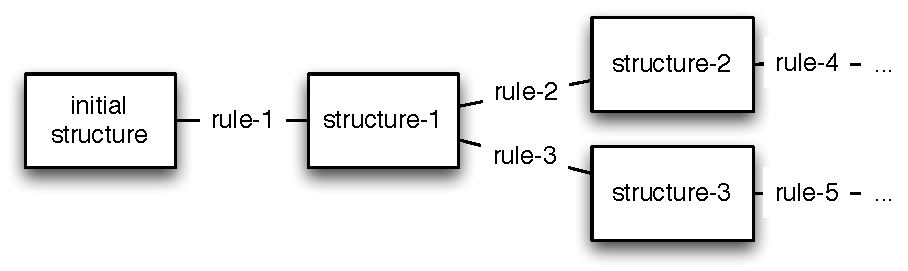
\includegraphics[width=.75\textwidth]{./frameworks/figures/fcg-search.pdf}
    \caption[Application of a rule-set]{Typical language processing in
      FCG is organised as a search process. A linguistic structure is
      being built up by applying a series of rules to it. When two
      (conflicting) rules could apply to the same structure, this
      leads to a split in the application tree.}
    \label{f:fcg-search}
  \end{center}
\end{figure}

\subsection{Coupled feature structures}
\label{s:coupled-feature-structures}
\is{coupled feature structure}

The linguistic structure that is being built up is represented as
\textsc{coupled feature structures}. Each coupled feature structure
consists of two feature structures or \textsc{poles}: one is defined in
the semantic domain and the other in the syntactic domain. Each
feature structure consists of a list of units, which are typically
reflected in both poles. Each unit consists of a list of feature-value
pairs which represent linguistic information. Special features,
\emph{sem-subunits} in the semantic pole and \emph{syn-subunits},
allow to specify hierarchical relations between units to construct
treelike relations between units.

FCG is open-ended to the features it can handle, but the features that
are typically used are: \emph{meaning}, \emph{referent}, and
\emph{sem-cat} in the semantic pole and \emph{form} and \emph{syn-cat}
in the syntactic pole. The \emph{meaning} feature refers to the
conceptual meaning of a certain unit, which can be expressed in any
formalism, including predicate logic or a semantic network in IRL. The
\emph{referent} is typically represented as a unique variable which is
bound to the (physical) entity that a unit (including all its
subunits) refers to. The \emph{form} feature contains all posible form
constraints, such as particular strings or word-order constraints
between its subunits. The \emph{syn-} and \emph{sem-cat} are
categories, either in the semantic or syntactic domain, that allow
other rules to specify which units to select for.

An example of a simplified linguistic structure for an utterance like
\textit{le ballon} is shown in Figure \ref{f:cfs-le-ballon} and its
bracketed notation is shown below. The semantic pole is shown on the
left and the syntactic pole on the right to show the structural
similarity between both poles.

\footnotesize
\ltitle{Example linguistic structure for "le ballon"}
\begin{lstlisting}
((top-unit                          ((top-unit
  (sem-subunits (det-np-unit)))       (syn-subunits (det-np-unit))
 (det-np-unit                        (det-np-unit
  (sem-subunits                       (syn-subunits 
   (ballon-unit le-unit))              (ballon-unit le-unit))
  (referent x)                        (form ((meets le-unit ballon-unit)))
  (meaning ((grounded x)))            (syn-cat 
  (sem-cat (object)))                  (determined-nounphrase)))
 (le-unit                            (le-unit 
  (referent x)                        (form 
  (meaning ((unique x)))               ((string le-unit "le")))
  (sem-cat (selector)))               (syn-cat (determiner)))
 (ballon-unit                        (ballon-unit 
  (referent x)                        (form 
  (meaning ((ball x)))                 ((string ballon-unit "ballon")))           
  (sem-cat (prototype))))             (syn-cat (noun))))
\end{lstlisting}
\normalsize

\begin{figure}[htbp]
  \begin{center}
    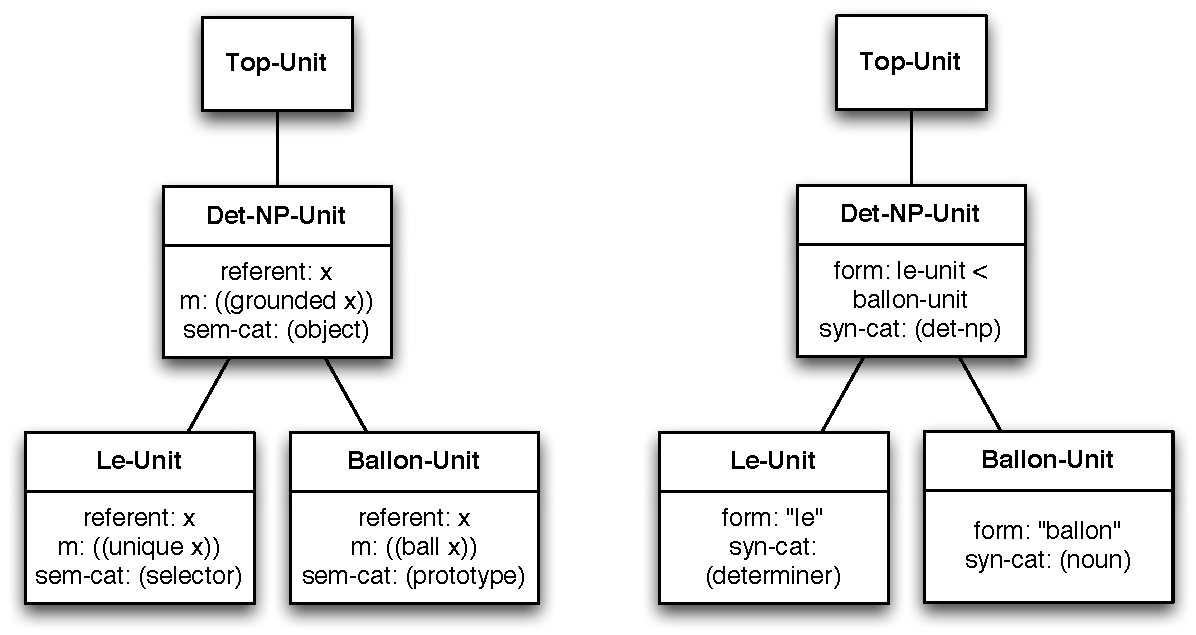
\includegraphics[width=.8\textwidth]{./frameworks/figures/cfs-le-ballon.pdf}
    \caption[Example coupled feature structure for \textit{le ballon}]{A
      graphical representation of the linguistic structure for \textit{le
      ballon}. The semantic pole is shown on the left, the syntactic
      pole on the right. Both poles are structurally very similar, but
      only contain features that are relevant in their domain.}
    \label{f:cfs-le-ballon}
  \end{center}
\end{figure}

\subsection{Application of a construction}

Now that we know how a linguistic structure is represented in FCG, we
can turn to the application of a construction to build up such a
structure. Like a linguistic structure, a construction is also
represented as a coupled-feature structure. The semantic pole of a
construction specifies how meaning has to be built up in parsing or
decomposed in production, and the syntactic pole how the form has to
be analysed in parsing or built in production. A construction also
typically contains more variables as it should be applicable to a wide
range of instantiated linguistic structures.

A construction is applied in three steps: a \textsc{matching phase}, a
\textsc{first merging phase} and a \textsc{second merging phase}. In
general, the matching phase checks whether the rule is applicable and
the two merging phases add new information to the linguistic structure
that is being built up. Although the matching phase is the most strict
one, all other phases can block the application of a rule if
conflicting information would already be present in the current
structure. More details on how matching and merging is exactly
implemented can be found in a background article
\citep{steels06unify}.

In production, it is the syntactic pole that is matched to the
syntactic pole of the current structure; in interpretation it is the
semantic pole that is matched to the current semantic pole. When the
matching phase has been successful, both poles of the rule are merged
into the current structure. The application of a rule is illustrated
in Figure \ref{f:fcg-rule-application}.

\begin{figure}[htb]
  \begin{center}
    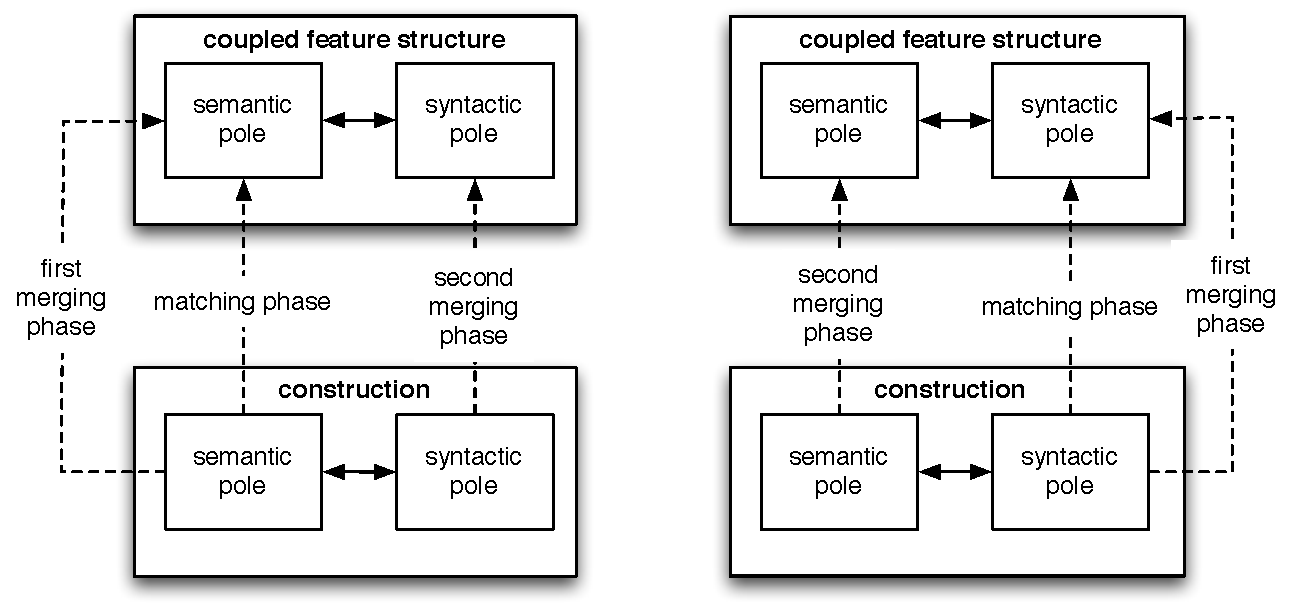
\includegraphics[width=\textwidth]{./frameworks/figures/fcg-rule-application.pdf}
    \caption[Application of a rule]{Rule application in FCG. Applying
      a rule consists of three phases: a matching phase and two
      merging phases. In production (left), the semantic pole is
      matched to check whether a rule is applicable. In interpretation
      (right), it is the syntactic pole that is matched. When the
      matching phase has been successful, both poles are merged into
      the coupled feature structure.}
    \label{f:fcg-rule-application}
  \end{center}
\end{figure}

\subsection{Structure building}
\is{FCG!structure building}
\is{structure building|see{FCG}}

The merging phases during the application of a construction can be
used to add new features to a unit or to add new values to a
particular feature of a particular unit, but more powerful structure
building operations are also possible. These operations can be used to
add new units to the structure, to change the hierarchy relations
between units and to move feature-value pairs from one unit to
another. All these operations are achieved through two operators: the
J-operator \citep{debeule05hierarchy} and the TAG-operator. The syntax
of these operators is shown below.


\footnotesize
\ltitle{Syntax of the TAG-Operator}
\begin{lstlisting}
(?unit
  (TAG ?tag-variable (feature-name feature-value)))
\end{lstlisting}

\ltitle{Syntax of the J-operator}
\begin{lstlisting}
((J ?focus-unit ?parent-unit (?child-unit-1 ... ?child-unit-n))
 ?tag-variable-1 
 ...
 ?tag-variable-n
 (feature-name-1 feature-value-1)
 ...
 (feature-name-n feature-value-n))
\end{lstlisting}
\normalsize

Units that are marked by the J-operator, or \textsc{J-units} for short,
are ignored in the matching phase, but receive special treatment
during the merging phase. The TAG-operator allows a construction to
bind a certain variable, \emph{?tag-variable}, to a certain
feature-value pair. Whenever this variable appears inside a J-unit of
the same rule, the bound feature-value pair will be moved to this
J-unit. The special treatment of a J-unit in the merging phase is as
follows:

\begin{enumerate}
\item if \emph{?focus-unit} is bound to a unit-name in the current
  structure, it will consider this unit to be in focus; if this
  variable is unbound, a new unit is created that will be in focus of
  this J-unit
\item the focus-unit will become a subunit of \emph{?parent-unit} and
  the optional \emph{?child-units} will become children of the
  focus-unit
\item the listed feature-value pairs will be merged into to the
  focus-unit
\item the feature-value pairs that are bound to the
  \emph{?tag-variables} will be moved from their original unit to the
  focus-unit
\end{enumerate}

\subsection{Linking through variable equalities}
\is{linking|see{FCG}}
\is{FCG!linking}

Once relations between several entities can be expressed in language,
hearers face an additional problem in figuring out what these
relations are. This is typically considered to be conveyed through
grammar. For example in a sentence like \textit{Jack hits Jill} English
grammar clearly conveys it is Jack who is the agent and Jill the
unfortunate recipient of the event, unlike the sentence \textit{Jill hits
Jack} in which the roles are reversed. Another example would be \textit{the
big block and the red ball} in which the hearer would need to figure
out it is the block which is big and the ball which is red. This
problem has been identified as the linking problem
\citep{steels05linking}.

In FCG this problem has been solved by first assuming that variables
introduced by different rules are different, but can be made equal
during the application of other grammatical rules. Let us consider the
phrase \textit{red ball} and assume the meaning is represented in predicate
logic. In parsing, the lexical constructions would introduce two
predicates, ``red(?x)'' and ``ball(?y)'', each introducing a different
variable. Another grammatical construction, which specifies that all
predicates referred to by adjectives and nouns that are part of the
same noun phrase should share the same variable, will make these
variables equal. The application of this rule transforms the
interpreted meaning in ``red(?x)'' and ``ball(?x)'' and hence solves the
linking problem for this small example.

\subsection{Application of an example construction}

I will now show the application of an example
NounAdjective-construction in interpretation. It illustrates both the
structure building operators and the linking problem. It will search
for two units, one of syntactical category \emph{noun} and the other
of syntactical category \emph{adjective} that occur next to each other
in the utterance parsed so far. When it has found two such units, it
introduces an intermediary unit and makes the variables of the
predicates in these two units equal through the referents of their
units. The coupled feature structure before and after application of
the construction is shown in Figure \ref{f:nounadj-application}.

\begin{figure}
  \begin{center}
    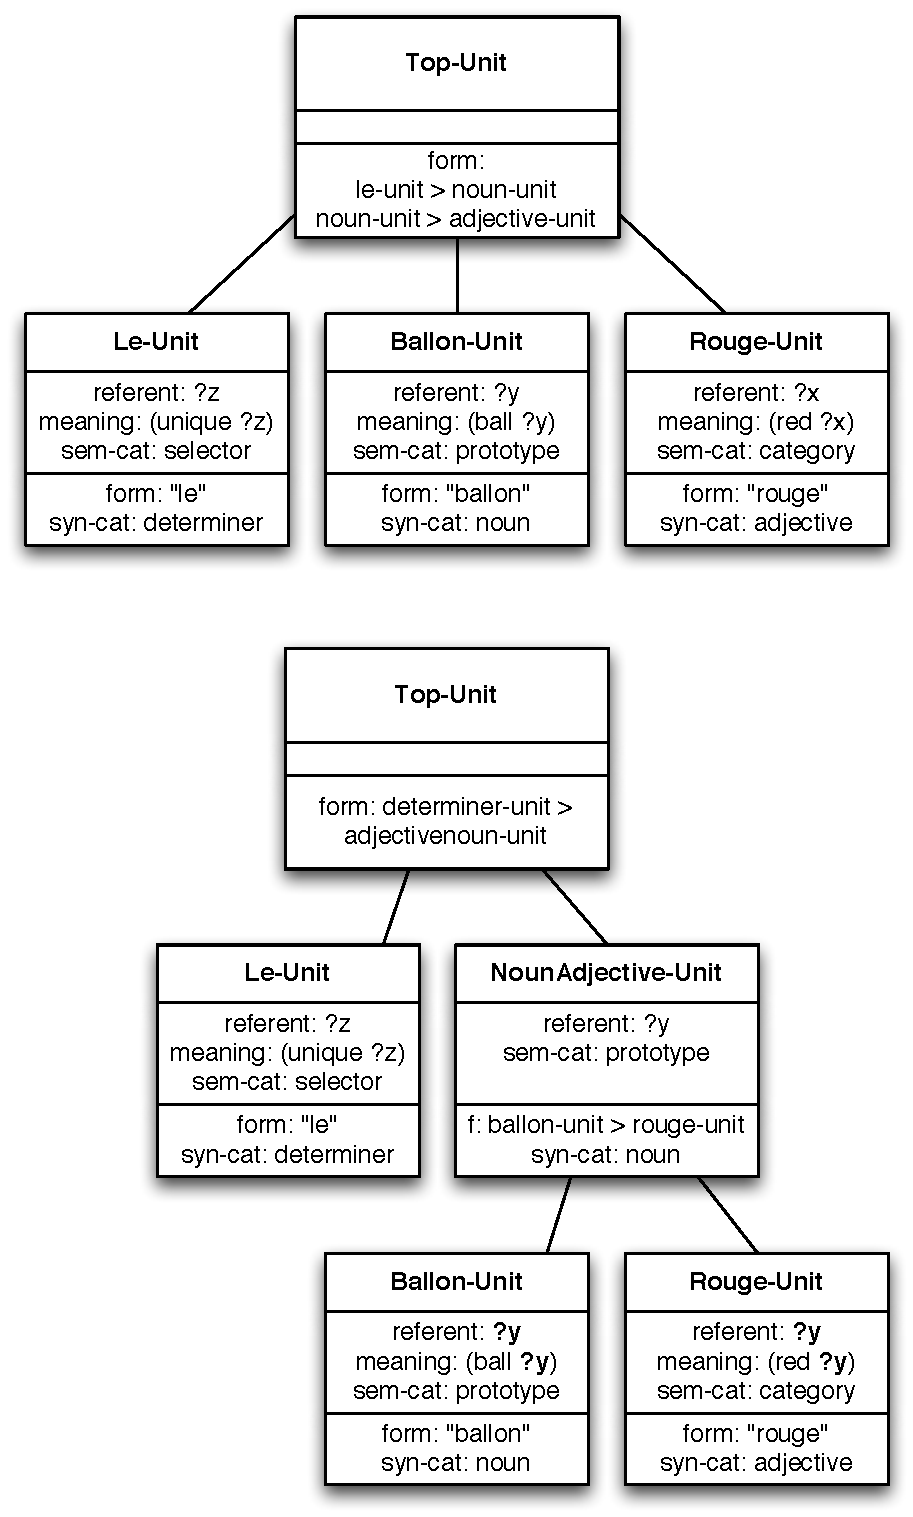
\includegraphics[width=.75\textwidth]{./frameworks/figures/nounadj-application.pdf}
    \caption[Coupled feature structures before and after the
    application of an example construction]{Coupled feature structures
      before (top) and after (bottom) the application of the
      NounAdjective construction in interpretation. It introduces a
      new unit which combines a Noun and an Adjective unit and makes
      the variables of their predicates equal through their
      referents. The coupled feature structures are now mapped on one
      structure which both contains semantic and syntactic
      information.}
    \label{f:nounadj-application}
  \end{center}
\end{figure}

I'll now step through the rule application of the rule in more
detail. In interpretation the utterance is de-rendered into a set of
form constraints: a set of strings, one for each word, and a set of
meets constraints between each consecutive pair of words. An example
for \textit{le ballon rouge} is given in the initial structure below. Note
that the semantic pole and syntactic pole are now shown under each
other and separated by a double arrow.

\footnotesize
\ltitle{Initial Structure}
\begin{lstlisting}
((top-unit))
<-->
((top-unit
 (form
   ((string le-unit "le")
    (string ballon-unit "ballon")
    (string rouge-unit "rouge")
    (meets le-unit ballon-unit)
    (meets ballon-unit rouge-unit)))))
\end{lstlisting}
\normalsize

Next the lexical constructions apply, which introduce for each string
a different unit (using the J-operator), which on the semantic side
introduces the corresponding meaning predicate together with their
referent and semantical category and on the syntactic side introduces
the appropriate syntactical categories. The coupled feature structure
after application of lexical constructions is shown below in bracketed
notation and in Figure \ref{f:nounadj-application} (top).

\footnotesize
\ltitle{Structure before application of the Noun-Adjective construction}
\begin{lstlisting}
((top-unit
  (sem-subunits (rouge-unit le-unit ballon-unit)))
 (rouge-unit
  (meaning ((red ?x)))
  (referent ?x)
  (sem-cat ((pom category))))
 (ballon-unit
  (meaning ((ball ?y)))
  (referent ?y)
  (sem-cat ((pom prototype))))
 (le-unit
  (meaning ((unique ?z)))
  (referent ?z)
  (sem-cat ((pom selector)))))
<-->
((top-unit
  (syn-subunits (rouge-unit le-unit ballon-unit))
  (form
   ((meets ballon-unit rouge-unit) 
    (meets le-unit ballon-unit))))
 (rouge-unit
  (form ((string rouge-unit "rouge")))
  (syn-cat ((pos adjective))))
 (le-unit 
  (form ((string le-unit "le"))) 
  (syn-cat ((pos determiner))))
 (ballon-unit
  (form ((string ballon-unit "ballon")))
  (syn-cat ((pos noun)))))
\end{lstlisting}
\normalsize

We are now ready to apply the Noun-Adjective construction which is
shown below. The first phase is the matching phase and as we are in
interpretation, this means the syntactic pole of the construction will
be matched against the syntactic pole of the current coupled feature
structure, which succeeds. There is only one adjective-unit and one
noun-unit, so this results one set of possible bindings:
\emph{((?parent-unit . top-unit) (?noun-unit . ballon-unit)
  (?adjective-unit . rouge-unit))}.

Matching succeeded, so we can now continue in the first merge phase,
in which the syntactic pole of the construction is merged into the
current feature structure. The syntactic pole contains only one J-unit
which will now be applied. As there is no binding for
\emph{?adj-noun-unit} yet, it will create a new unit that will be a
child of \emph{?parent-unit} (which in this application will be
\emph{top-unit} as can be seen in the bindings of the unification
phase) and which will have two children: \emph{ballon-unit} and
\emph{rouge-unit}. The feature-value pairs specified in the J-unit,
namely the syntactical category noun, will be added to this
unit. Finally the tag-variable \emph{?form} will be handled, which
moves the meets constraint between the \emph{ballon-unit} and the
\emph{rouge-unit} from \emph{top-unit} to the newly created unit.

\footnotesize
\ltitle{The Noun-Adjective construction}
\begin{lstlisting}
((?parent-unit
  (sem-subunits (== ?noun-unit ?adjective-unit)))
 (?noun-unit 
  (referent ?x) 
  (sem-cat (==1 (pom prototype))))
 (?adjective-unit
  (referent ?x)
  (sem-cat (==1 (pom category))))
 ((J ?adj-noun-unit ?parent-unit (?noun-unit ?adjective-unit))
  (referent ?x)
  (sem-cat (==1 (pom prototype)))))
<-->
((?parent-unit
  (syn-subunits (== ?noun-unit ?adjective-unit))
  (tag
   ?form
   (form (== (meets ?noun-unit ?adjective-unit)))))
 (?noun-unit 
  (syn-cat (==1 (pos noun))))
 (?adjective-unit 
  (syn-cat (==1 (pos adjective))))
 ((J ?adj-noun-unit ?parent-unit (?noun-unit ?adjective-unit))
  ?form
  (syn-cat (==1 (pos noun)))))
\end{lstlisting}
\normalsize

In the final merging phase, the semantic pole of the construction is
merged into the semantic pole of the current feature structure. Next
to creating a new unit similar to the unit created in the syntactic
pole, it ensures the variables of the predicates for ball and red will
be made equal. In the current structure they are available as the
referent of the \emph{ballon-unit} and the \emph{rouge-unit}, which
are equal in the \emph{?adjective-unit} and the \emph{?noun-unit} of
the Noun-Adjective construction. The merging phase will ensure that
these variables are equalised in the resulting feature structure,
which is shown below and in Figure \ref{f:nounadj-application}
(bottom).

\footnotesize
\ltitle{Structure after application in interpretation}
\begin{lstlisting}
((top-unit
  (sem-subunits (noun-adj-unit le-unit)))
 (noun-adj-unit
  (sem-subunits (rouge-unit ballon-unit))
  (referent ?y)
  (sem-cat ((pom prototype))))
 (le-unit
  (meaning ((unique ?z)))
  (referent ?z)
  (sem-cat ((pom selector))))
 (ballon-unit
  (meaning ((ball ?y)))
  (sem-cat ((pom prototype)))
  (referent ?y))
 (rouge-unit
  (meaning ((red ?y)))
  (sem-cat ((pom category)))
  (referent ?y)))
<-->
((top-unit 
  (syn-subunits (noun-adj-unit le-unit))
  (form ((meets le-unit noun-adj-unit))))
 (noun-adj-unit
  (form ((meets ballon-unit rouge-unit)))
  (syn-subunits (rouge-unit ballon-unit))
  (syn-cat ((pos noun))))
 (rouge-unit
  (form ((string rouge-unit "rouge")))
  (syn-cat ((pos adjective))))
 (le-unit 
  (form ((string le-unit "le"))) 
  (syn-cat ((pos determiner))))
 (ballon-unit
  (form ((string ballon-unit "ballon")))
  (syn-cat ((pos noun)))))
\end{lstlisting}
\normalsize


\part{Language strategies for colour}\label{s:language-strats}

\section*{Introduction}

In the first part of this book, I will introduce the semantic and
syntactic templates of various language strategies that have been
introduced in Section \ref{s:strats-for-colour}. For each of these
strategies, I will implement a predefined language system that will
allow me to evaluate the performance of the proposed semantic and
syntactic templates. The strategies will be compared to human language
systems using \emph{naming benchmarks}, and these strategies will be
compared to each other in a \emph{baseline experiment}.

A compositional approach is applied to both
\emph{semantic}\is{semantic template} and \emph{syntactic
  templates}\is{syntactic template}. This implies that parts of the
templates will be shared by various strategies. The semantic templates
will be represented by semantic constraint networks (see Section
\ref{s:semantic-constraint-network}). These networks consist of
semantic primitives which will be explained in more detail for each
strategy. The syntactic templates will be presented as a general
approach to expressing these semantic networks in language. These
templates will be illustrated by giving examples of coupled feature
structures (see Section \ref{s:coupled-feature-structures}), which
allow to express the semantic constraint networks in language. Example
constructions are described that can build up these coupled feature
structures \citep{bleys06next, steels07emergence, bleys08expressing}.

Natural language systems are implemented by providing actual
ontologies and linguistic inventories to express these ontologies in
language. For the basic colour strategy, this boils down to providing
agents with an ontology of categories that are reported in literature,
the lexical rules for that ontology, and the grammatical rules to
express the instantiated semantic template.

The implementation of natural language systems will allow for the
evaluation of the proposed templates. A first evaluation method is to
name a set of colour samples whose names have been reported in
literature in a \emph{naming benchmark}\is{naming benchmark}. 
Comparing the names produced by the strategy to the
expected names gives a rough idea of how well the templates reflect
the natural system. A second evaluation method is a \emph{baseline
  experiment}\is{baseline experiment} in which agents, equipped
with the implementation of the natural language system, involve in
colour naming games (see Section
\ref{s:language-games-for-colour}). This allows for a comparison of
the performance of the templates across language strategies.

\newpage
\thispagestyle{empty}

\chapter{Basic colour strategy}
\label{s:basic-strategy}
\label{s:first-strategy}
\is{language strategy!for colour!basic colour strategy}
\is{basic colour strategy|see{language strategy}}

The basic colour strategy is by far the most studied language
strategy for the domain for colour. It stipulates that a colour should
be described using a single colour term that refers to a single colour
category. At the semantic level it specifies how the categorisation
process should be organised; at the syntactic level it specifies how
these categories should be expressed in language. As this strategy has
been studied extensively in the domain of artificial language
modelling, it allows me to establish a solid common base before moving
on to the other strategies.

\section{Related research}

\subsection{Colour categories}

Colour categories\is{colour category} are considered to be
prototypical in nature \citep{rosch73natural}. One colour sample, the
\textsc{prototype}\is{prototype|see{colour category}}, is considered
to be the best example of a certain category and membership to this
category is graded: some samples are considered to be better members
of a certain category than others. A bluish shade of green is for
example considered to be a worse example of the category of green than
the natural colour of grass.

\subsubsection{Determining location of basic colour categories}

Part of the research in colour cognition aims at locating the typical
member of each colour category of the category systems in different
natural languages, such as Spanish \citep{lillo07locating}, English
\citep{boynton87locating, sturges95location} and Russian
\citep{safuanova07russian}. These experiments typically involve naming
a set of individual colour samples.

In colour literature, the distinction is made between the \textsc{focus}
(the colour sample which is named fastest) and the \textsc{centroid}
(the colour central to all colours that belong to the category) of a
colour category. Interestingly, a discrepancy exists between the
locations of these two \citep{sturges95location}. Some of the
experiments also reported on \textsc{consensus samples}\is{consensus
  samples|see{colour category}}, which are samples that were
consistently named by all participants in the experiment. The
consensus samples for English \citep{sturges95location} are shown in
Figure \ref{f:basic-consensus-chips-english}.

\begin{figure}[htbp]
  \begin{center}
    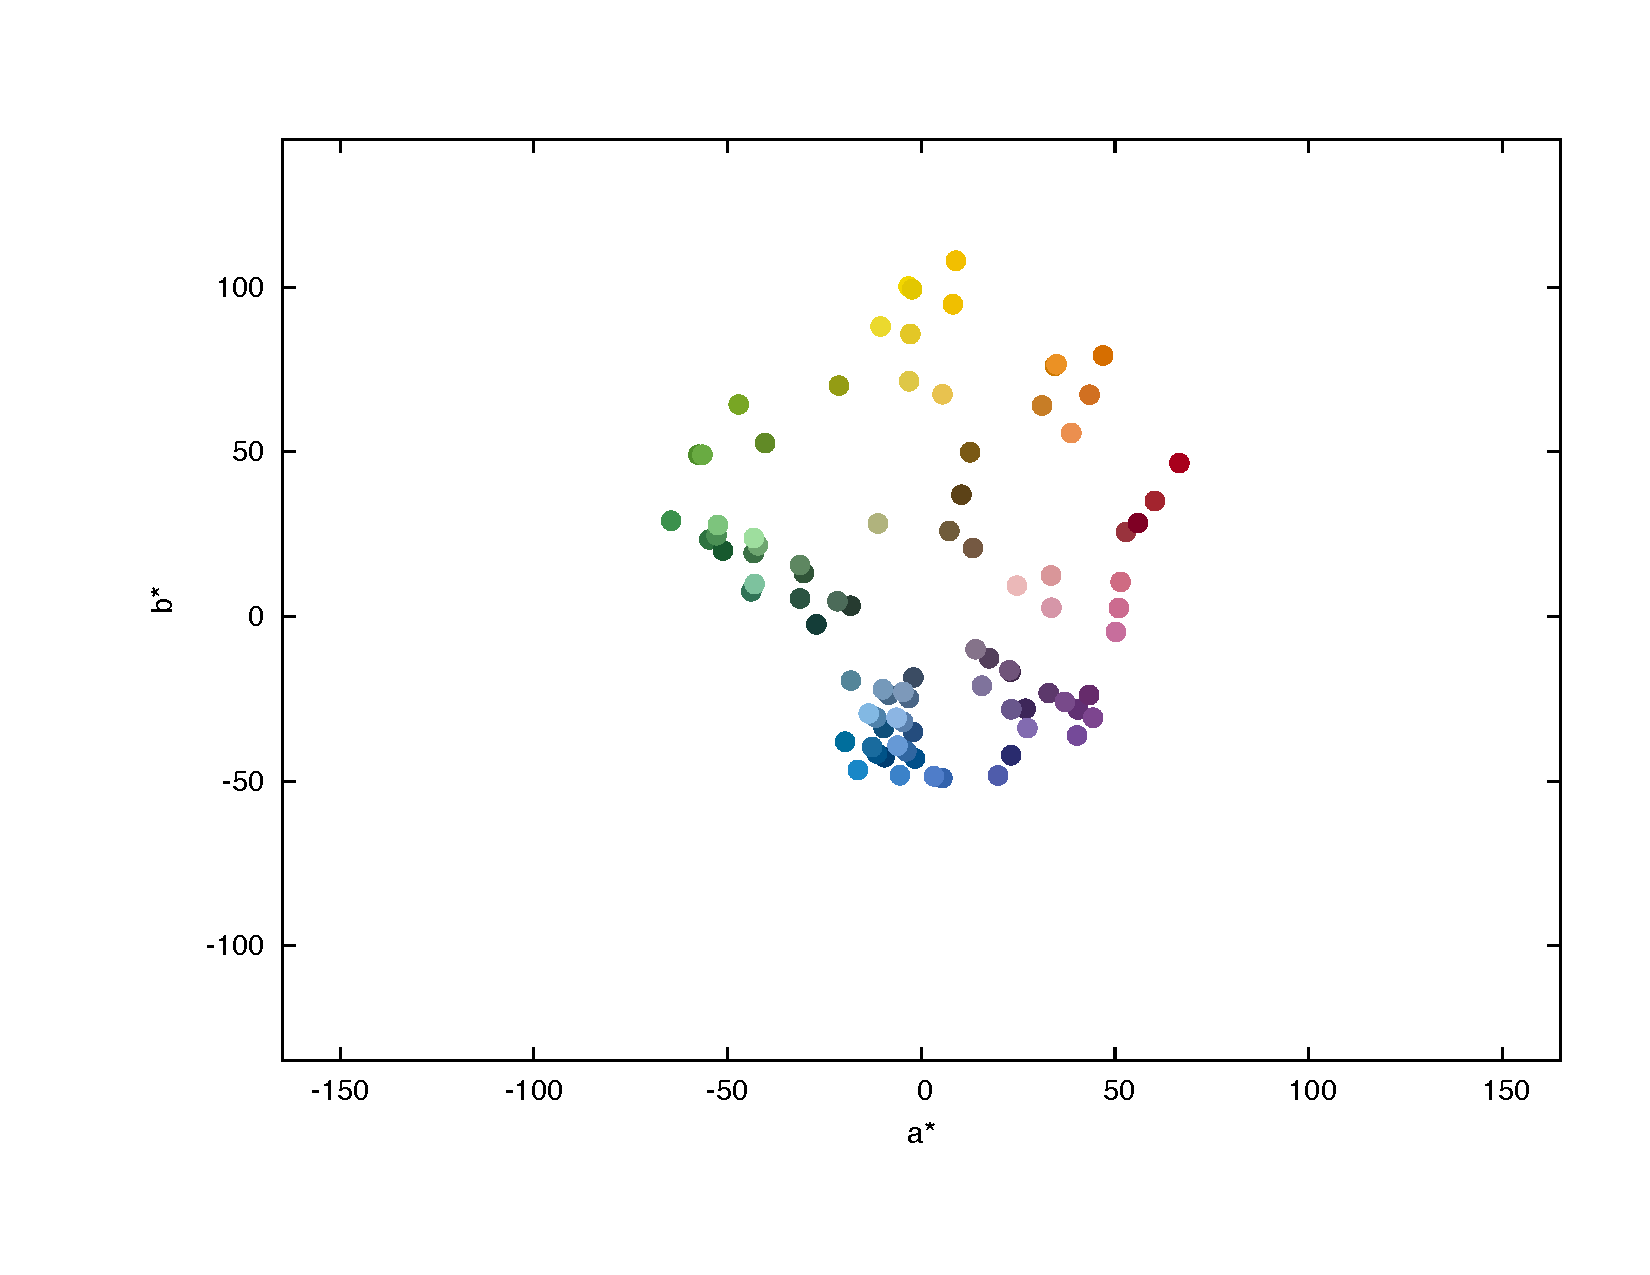
\includegraphics[width=.8\textwidth]{./basic-strategy/figures/sturges-consensus-chips.pdf}
    \caption[Consensus chips for English]{The consensus chips (all
      samples that were consistently named by all participants) for
      English \citep{sturges95location}.}
    \label{f:basic-consensus-chips-english}
  \end{center}
\end{figure}

\subsection{Models}

The basic colour strategy has received quite some attention
within the field of artificial language evolution. Most of these
studies adhere to the the language game paradigm and use the colour
naming game (see Section \ref{s:language-games-for-colour}) to study
how a population of agents could coordinate their own colour category
system. Although there seems to be a high coherence in the models that
have been proposed for this game, different implementation choices
have been made. Colour categories were represented either as radial
basis function networks \citep{steels05coordinating}, single points in
a three dimensional conceptual space \citep{belpaeme05explaining,
  belpaeme07language} or a set of points sharing the same linguistic
label in a one dimensional conceptual space \citep{puglisi08cultural,
  baronchelli10modeling}. A comparison between the different
implementations of the basic colour strategy is shown in Table
\ref{t:language-game-models-comparison}.

\renewcommand{\arraystretch}{1.5}
\begin{table}[htbp]
\resizebox{\textwidth}{!}{
%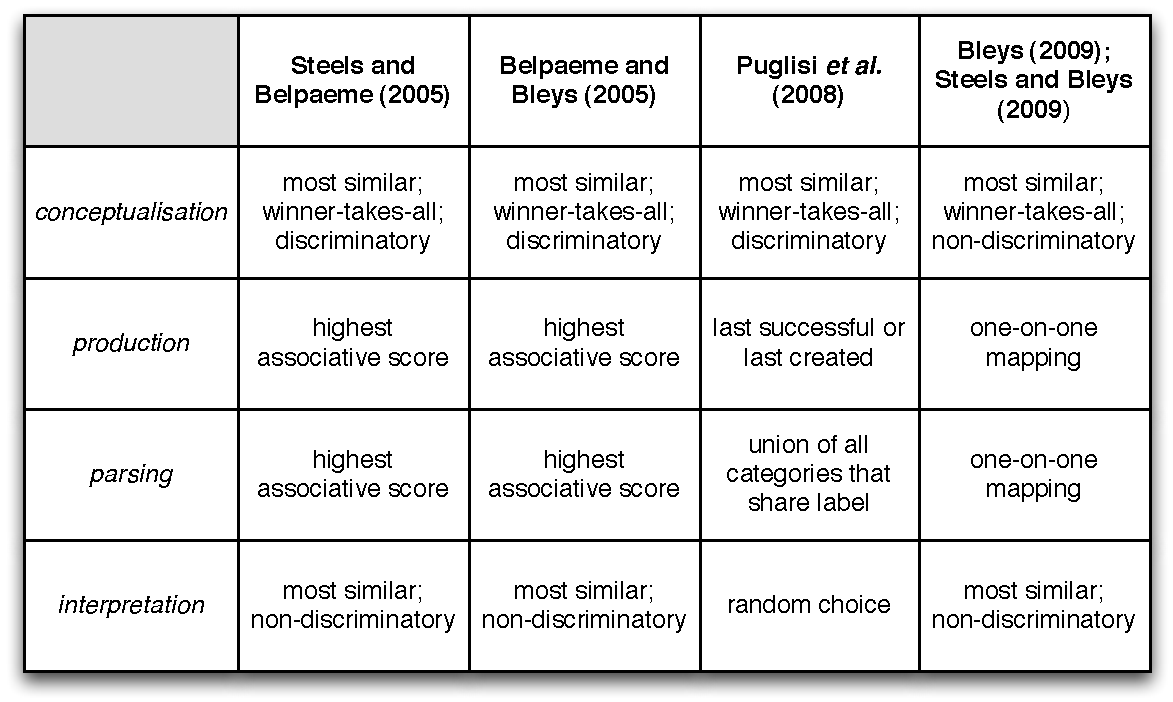
\includegraphics[width=\textwidth]{./basic-strategy/figures/language-game-models-comparison}
  \begin{tabular}{>{\centering\arraybackslash}m{.2\textwidth}>{\centering\arraybackslash}m{.275\textwidth}>{\centering\arraybackslash}m{.275\textwidth}>{\centering\arraybackslash}m{.275\textwidth}>{\centering\arraybackslash}m{.275\textwidth}}
  \lsptoprule
  & \citet{steels05coordinating} & \citet{belpaeme05explaining} & \citet{puglisi08cultural} & Bleys (2009);\newline \citet{bleys09linguistic} \\
  \midrule
  \textsc{conceptual\-isation} & most similar; winner-takes-all; discriminatory & most similar; winner-takes-all; discriminatory & most similar; winner-takes-all; discriminatory & most similar; winner-takes-all; non-discriminatory \\\hline
  \textsc{production} & highest associative score & highest associative score & last successful or last created & one-on-one mapping \\\hline
  \textsc{parsing} & highest associative score & highest associative score & union of all categories that share label & one-on-one mapping \\\hline
  \textsc{inter\-pretation} & most similar; non-discriminatory & most similar; non-discriminatory & random choice & most similar; non-discriminatory \\
  \lspbottomrule
  \end{tabular}
 }
  \caption[Comparison of the different models for the basic colour
  strategy]{Comparison of the different models for the basic colour
    strategy.}
  \label{t:language-game-models-comparison}
\end{table}
\renewcommand{\arraystretch}{1}
\todo{Bleys 2009 is not in bib}

\section{Semantic template}
\label{s:bs-semantic-template}
\is{semantic template!for basic colour strategy}

In previous models of the colour naming game
\citep{steels05coordinating, belpaeme05explaining, puglisi08cultural}
the speaker selected the category that was most similar to the topic
entity. Additionally this category needed to be discriminatory in the
current context: no other entity in the context should be categorised
as belonging to the same category as the topic. In general, the hearer
was more lenient: it selected the entity that was most similar to the
interpreted category, regardless of whether it would actually be
classified as the interpreted category and whether other entities
would be classified as the same category. So for example, the hearer
would select an orange entity when interpreting the yellow colour
category even if it would know a colour category for orange. Previous
research has shown the negative impact of applying the discriminatory
criterion as a hearer, especially when the category systems of the
agents are not aligned \citep{belpaeme07language}.

The semantics I propose in this book adhere to the main ideas
proposed by the previous models, but with a minor difference. The
speaker still selects the category that is most similar to the topic
entity and the hearer will point to the entity that is most similar to
the interpreted category. The speaker however is a bit more lenient as
it does not apply the discriminatory criterion. This will result in a
higher level of communicative success, as the speaker will now be able
to successfully name entities that are most similar to a category,
even if this category is not discriminatory. For example, if the
context contains two green colour samples, the sample that is most
similar to the green colour category can still be successfully
named. 

The semantic template of the basic colour strategy can be
summarised in three steps: profiling, categorisation and
selection. These processes are represented separately in semantics as
this will enhance possible re-use of these primitives in other
strategies.

\subsection{Profiling}
\is{profiling}

During the categorisation process, some dimensions of the colour
domain might have a bigger impact than others (see Section
\ref{s:intro-basic-colour-strategy}). In order to represent this in
semantics, I need primitives that will \emph{profile}, or highlight,
some dimensions of a particular colour sample before the
categorisation process. For each strategy reported in the literature
review, I define a different primitive.

This profiling could also instruct the vision system of a robotic
agent to process the colour information of the objects. This could
defer the computation of the different features of the objects until
they become absolutely necessary.

\subsection{Categorisation based on colour}
\label{s:bcs-categorisation}

As the main psychological theory for categorisation, I have chosen to
follow the prototype-based approach to colour categories as advocated
by \cite{rosch73natural}. In this theory, a category is defined by its
prototype. This prototype serves as the best sample of a category and
is compared to a particular colour sample to determine the graded
membership of this sample to this category.

Both colour samples and prototypes of colour categories are
represented in the CIE $L^*a^*b^*$ (see Section \ref{s:lab}) colour
space. This colour space turned out to be the best space in a related
model of colour naming \citep{lammens94computational} and is
\emph{equidistant}: Euclidean distance between colours represented in
this space reflects psychological differences as perceived by humans.

Similarity can thus be expressed as an exponentially decaying function
\citep{shepard87toward, gardenfors04conceptual} of the weighted
distance between the prototype of a colour category and a colour
sample (as shown in Equation \ref{e:similarity}). In this function,
$c$ is a sensitivity parameter. As in the current simulations this
parameter is identical for all colour categories, the actual value of
this parameter does not result in any qualitatively different
results. It is possible to imagine simulations in which the
sensitivity parameter is different for each colour category, so that some 
categories cover a relative larger area of the
colour space than others. The distance is weighted in each dimension by the
product of the current profile of the entity and the weights of the
prototype of the colour category. The weights of a prototype reflect
the importance of each dimension for that category. Some categories,
such as the basic colour categories, are defined in all dimensions,
whereas others are only defined in some dimensions (such as the
lightness dimension for the categories for light and dark). The exact
equation is shown in Equation \ref{e:weighted-distance}.

\begin{align}
s(i,j) &= e^{-cd_w(i,j)}
\label{e:similarity} \\
d_w(x,y) &= \sqrt{\sum_{k=1}^n w_{x_k}w_{y_k} (x_k - y_k)^2}
\label{e:weighted-distance}
\end{align}

\subsection{Selection based on activation}

An activation value is assigned to each entity, which reflects the
similarity of that entity to the category that was used during the
categorisation process. The more similar the entity was to the
category, the higher the activation will be. The entity with the
highest activation will be selected as the outcome of the complete
process.

\subsection{Semantic constraint network}

The semantic constraint network for the basic colour strategy is shown
in Figure \ref{f:bcs-semantic-structure}. The {\sc
  Equal-to-Context} primitive introduces all entities in the sensory
context of the agent. The {\sc Profile-Colour-Dimensions} primitive
sets the focus to each entity in the context based on the dimension
profiler that is bound to its third slot. The {\sc
  Filter-by-Colour-Lenient} primitive performs the categorisation
process based on the colour categories known to the agent and assigns
an activation score of the remaining entities. Finally, {\sc
  Select-Most-Activated} selects the entity with the highest
activation from the set of activated entities.

Whether the {\sc Filter-by-Colour-Lenient} primitive selects a subset
of entities from its input set depends on whether the argument for its
colour category is already bound. During conceptualisation, the
argument for the colour category will typically be unbound and hence
the primitive will divide the entities of the context in different
subsets. In interpretation however, the colour category is already
known and will be used to set the activation of all the entities in
the context.

\begin{figure}
  \begin{center}
    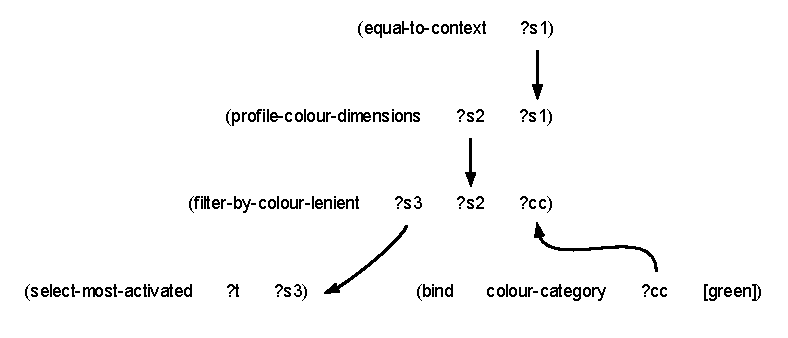
\includegraphics[width=.8\textwidth]{./basic-strategy/figures/semantics-interpretation.pdf}
    \caption[The semantic constraint network for the basic colour
    strategy]{The semantic constraint network for the basic colour
      strategy. The {\sc Profile-Colour-Dimensions} primitive profiles
      some dimensions in the context. {\sc Filter-by-Colour-Lenient}
      performs the the categorisation process and assigns activation
      values to the entities. The {\sc Select-Most-Activated}
      primitive will select the entity with the highest activation.}
    \label{f:bcs-semantic-structure}
  \end{center}
\end{figure}

\subsection{Semantic primitives}

\definition{Semantic primitive}{Equal-to-Context}

\begin{explanation}{description}
Retrieves all entities from in the sensory context and collects them in an entity set.
\end{explanation}

\begin{explanation}{arguments}
\verb+?context+ (of type entity-set)
\end{explanation}

\begin{explanation}{revision specs}
$\emptyset$: collects all entities in the sensory context in an entity set and binds it to \verb+?context+
\end{explanation}

\definition{Semantic primitive}{Profile-Colour-Dimensions}

\begin{explanation}{description}
Profiles the colour dimensions of the entities in an entity set.
\end{explanation}

\begin{explanation}{arguments}
\verb+?profiled-set+ (of type entity-set) \\
\verb+?source-set+ (of type entity-set)
\end{explanation}

\begin{explanation}{revision specs}
  \verb+?source-set+: profiles all colour dimensions of the entities
  in the entity set and binds the resulting entity-set to
  \verb+?profiled-set+
\end{explanation}

\begin{explanation}{note}
  Other variants of this primitive which profile other dimensions are
  defined as well. {\sc Profile-Brightness-Dimension} profiles only in
  the $L^*$ dimension and {\sc
    Profile-Brightness-and-Red-Green-Dimensions} profiles both the
  $L^*$ and $a^*$ dimension.
\end{explanation}

\definition{Semantic primitive}{Filter-by-Colour-Lenient}

\begin{explanation}{description}
  Applies a colour category to a set of entities. When the colour
  category is known, this primitive sets the activation of each entity
  in the set to the similarity between the entity and the
  category. When the colour category is unknown, it categorises the
  entities in the set to the category that is most similar to it.
\end{explanation}

\begin{explanation}{arguments}
\verb+?categorised-set+ (of type entity-set) \\
\verb+?source-set+ (of type entity-set) \\
\verb+?colour-category+ (of type colour-category)
\end{explanation}

\begin{explanation}{revision specs}
  \verb+?source-set ?colour-category+: sets the activation of the
  entities in the source set to the similarity to the colour category
  and binds the resulting entity-set to \verb+?categorised-set+ \\
  \verb+?source-set+: categorises each entity in the source set to the
  category that is most similar to it and returns pairwise bindings
  for \verb+?colour-category+ and \verb+?categorised-set+
\end{explanation}

\definition{Semantic primitive}{Select-Most-Activated}

\begin{explanation}{description}
Selects the entity from an entity-set that has the highest activation.
\end{explanation}

\begin{explanation}{arguments}
\verb+?entity+ (of type entity) \\
\verb+?entity-set+ (of type entity-set)
\end{explanation}

\begin{explanation}{revision specs}
\verb+?entity-set+: selects the entity from the entity-set with the highest activation and binds it to \verb+?entity+
\end{explanation}

\section{Syntactic templates}
\label{s:bcs-syntactic-templates}

The next question I have to address is how these semantic constraint
networks will be expressed in a serial utterance. When the hearer
parses this utterance, it should be able to fully reconstruct the
constraint network that the speaker wanted to transfer. 

The main approach adopted to express semantic networks in language is
outlined as follows. The semantic network is divided in three layers
of units: (a) entity units containing the semantic entities, (b)
functional units which make direct use of such a semantic entity and
(c) contextual units which contain any remaining operations of the
semantic constraint network that do not make direct use of any
semantic entity. This division is illustrated in Figure
\ref{f:bcs-linguistic-structure}.

\begin{figure}[htbp]
  \begin{center}
    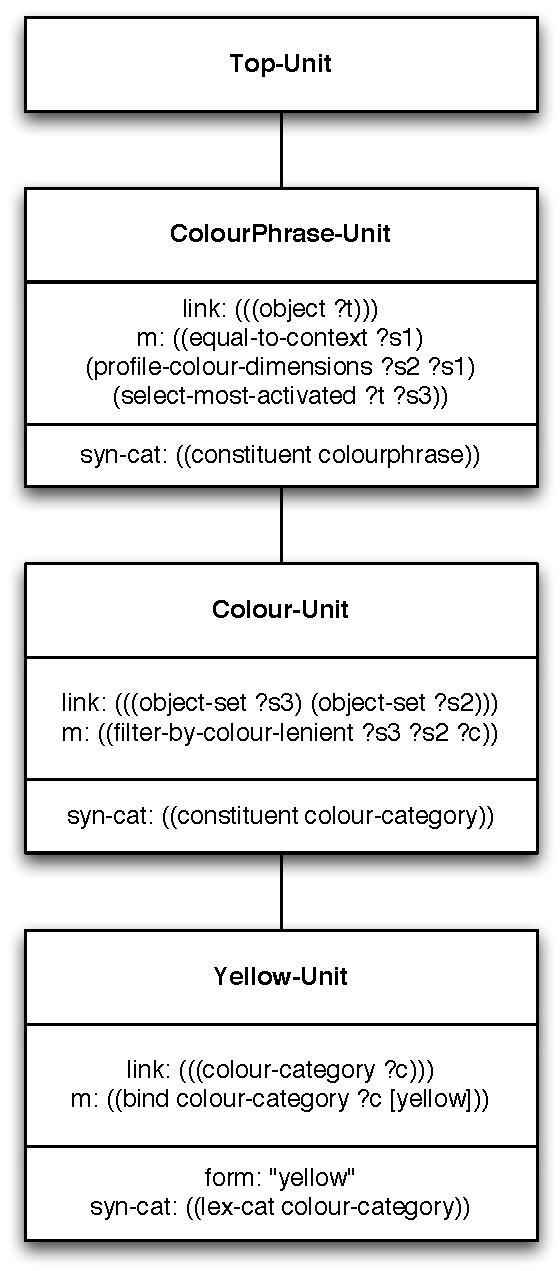
\includegraphics[width=.5\textwidth]{./basic-strategy/figures/linguistic-structure.pdf}
    \caption[Example linguistic structure for basic colour
    strategy]{Example linguistic structure for \texttt{colour-network 1}. The semantic constraint network is divided over three
      layers of units: one for the semantic entity [yellow], one for
      the functional primitive \textsc{Filter-by-Colour-Lenient} and
      one contextual unit for all other primitives of the semantic
      constraint network. The link feature links the variables for the
      entities and entity-set. Similarly, the c-link feature passes
      the variables for colour categories and sets of colour
      categories.}
    \label{f:bcs-linguistic-structure}
  \end{center}
\end{figure}

As a rule of thumb, the reader can assume that each rule introduces
one new unit in the linguistic structure. In production, syntactic
information is added to the structure: which words will be used to
express certain semantic entities, to which syntactic category does
each unit belong and which word order should be applied when this tree
is transformed into an utterance. During interpretation, each word in
the utterance introduces a new semantic entity. Based on the lexical
categories of these entities, the hearer is able to add the layer of
functional units. Finally, the information on the word order
constraints augmented with the information of the syntactic categories
allows the agent to select the right contextual rule. This rule adds
extra primitive constraints to the network, but more importantly also
connects all primitive constraints by introducing variable equalities
(for example between the first argument of
\textsc{Filter-by-Colour-Lenient} and the second argument of
\textsc{Select-Most-Activated}) in the network shown in Figure
\ref{f:bcs-semantic-structure}.

The syntactic templates specify the rules to express a semantic
network in a serial utterance. I will now discuss each step in more
detail. Three templates (1.1 to 1.3) take care of creating the rules
that ensure the default division in three layers of units: (a) entity
units containing the semantic entities, (b) functional units which
contain primitives that make direct use of such a semantic entity and
(c) contextual units which contain any other primitives that do not
make direct use of semantic entities.

\subsection{Syntactic template 1.1: Semantic entities}
\is{syntactic template!for semantic entities}

A semantic entity is an entity from the ontology used by a primitive,
such as a category, a prototype, a relation, etc. They have an
identifier which is created when the entity itself is constructed and
which can be used in a lexical rule. In parsing, the resulting rule
will also introduce a new variable that will allow the entity to be
used by other primitives in the network. To ensure this linking is
possible, the variable needs to be part of the link feature of that
unit.

An example of a lexical rule for the colour category yellow is given
below. The main association is between the category for yellow and the
string ``yellow''. Additionally, the rule adds a link feature to the
semantic side that enables other units to incorporate this semantic
entity in the rest of the semantic network. This rule is responsible
for introducing the Yellow-Unit in Figure
\ref{f:bcs-linguistic-structure} both in production and in parsing.

\footnotesize
\begin{Verbatim}[frame=lines, label=Entity rule for yellow]
((?top-unit
  (tag ?meaning 
       (meaning ((bind colour-category ?c [yellow])))))
 ((J ?yellow-unit ?top-unit)
  ?meaning
  (link (((colour-category ?c))))))
<-->
((?top-unit
  (tag ?form 
       (form ((string ?yellow-unit "yellow")))))
 ((J ?yellow-unit ?top-unit)
  ?form
  (syn-cat ((lex-cat colour-category)))))
\end{Verbatim}
\normalsize

\subsection{Syntactic template 1.2: Functional primitives}
\is{syntactic template!for functional primitives}
\is{functional primitive|see{primitive constraint}}
\is{primitive constraint!functional primitive}

Functional units, created by functional rules, handle
the primitives in a semantic network that directly use a semantic
entity. For each such primitive a separate functional rule is
created. The template to express such a primitives has a subunit for
each of its arguments. The functional unit that will be introduced by
this rule contains the functional primitive that needs to be covered.
As the other arguments of the primitive are not provided by the entity
unit, these arguments become available in the link of the new
functional unit. This link ensures the encapsulated primitive can be
incorporated in a larger semantic network.

An example of such a rule for the \textsc{Filter-by-Colour-Lenient}
primitive is given below. It uses a colour-category $?c$ , for example
the prototype for yellow, from the set of colour categories $cs$ to
filter some elements from a source set $?s2$ to yield a subset of
blocks $?s1$. It associates this primitive to a newly invented
syntactic constituent category (constituent colour-category).  The
variable of the colour category is linked in through the link feature 
specified in the subunit. The new unit will have the two object-sets,
$?s1$ and $?s2$, as values for the link feature 
as these yet need to be covered by
another rule. The resulting rule is shown below.

\footnotesize
\begin{Verbatim}[frame=lines, label=Functional rule for Filter-by-Colour-Lenient]
((?top-unit
  (sem-subunits (?colour-category-unit)) 
  (tag ?meaning
       (meaning ((filter-by-colour-lenient ?s3 ?s2 ?c)))))
 (?colour-category-unit 
  (link (((colour-category ?c)))))
 ((J ?filter-by-colour-unit ?top-unit (?colour-category-unit))
  ?meaning
  (link (((entity-set ?s3) (entity-set ?s2))))))
<-->
((?top-unit 
  (syn-subunits (?colour-category-unit)))
 (?colour-category-unit 
  (syn-cat ((lex-cat colour-category))))
 ((J ?filter-by-colour-unit ?top-unit (?colour-category-unit))
  (syn-cat ((constituent colour-category)))))
\end{Verbatim}
\normalsize

\subsection{Syntactic template 1.3: Contextual primitives}
\label{s:bcs-contextual-primitive}
\is{syntactic template!for contextual primitives}
\is{contextual primitive|see{primitive constraint}}
\is{primitive constraint!contextual primitive}

The primitives that do not make direct use of semantic entities are
grouped together in a contextual unit. This unit is introduced
by the application of a contextual rule, which contains
subunits for each of the functional primitives. It uses the link
feature of each of its subunits to ensure the primitives will be
incorporated in the primitives it contains. The unit that is
introduced will have as link feature the target entity of the semantic
constraint network it captures.

An example of such a rule for the contextual primitives of the
semantic network shown in Figure \ref{f:bcs-semantic-structure} is
given below. It encapsulates three primitives,
\textsc{Equal-To-Context}, \textsc{Profile-Colour-Dimensions} and
\textsc{Select-Most-Activated}. It requires one subunit to be present
in the structure which belongs to the syntactic category Constituent
Colour-Category and which has as link feature of two object sets. In
parsing, it will ensure the variables in these links are made equal to
the variables of the semantic primitives it contains. The newly
introduced unit will be of a newly invented syntactic category,
Constituent ColourPhrase, and will have as link feature the first
argument of the \textsc{Select-Most-Activated} primitive.

\footnotesize
\begin{Verbatim}[frame=lines, label=ColourPhrase rule for basic colour strategy]
((?top-unit
  (sem-subunits (?colour-unit))
  (tag ?meaning
       (meaning ((select-most-activated ?t ?s3)
                 (profile-colour-dimensions ?s2 ?s1)
                 (equal-to-context ?s1)))))
 (?colour-unit
  (link (((entity-set ?s3) (entity-set ?s2)))))
 ((J ?colourphrase-unit ?top-unit (?colour-unit))
  ?meaning
  (link (((colour-entity ?t))))))
<-->
((?top-unit 
  (syn-subunits (?colour-unit)))
 (?colour-unit 
  (syn-cat ((constituent colour-category))))
 ((J ?colourphrase-unit ?top-unit (?colour-unit))
  (syn-cat ((constituent colourphrase)))))
\end{Verbatim}
\normalsize

\section{Baseline experiment}
\label{s:basic-baseline-experiment}
\is{baseline experiment!for basic colour strategy}

A first test whether the proposed templates are valid is provided by a
naming benchmark\is{naming benchmark!for basic colour strategy}. It
involves naming all consensus chips for English
\citep{sturges95location} and verifying whether the resulting names
corresponds to those reported in literature. This benchmark is only
performed for the language system that is based on the centroids of
English \citep{sturges95location}. The results are shown in Table
\ref{t:bcs-naming-benchmark}. The benchmark reaches only around 83\%
success.  This suggests that, although capable of accounting for more
than three quarters of the consensus chips, the one-nearest neighbour
classification algorithm might be too general to capture all the
richness of human colour categories.

\begin{table}[htbp]
  \centering
  \resizebox{.85\textwidth}{!}{
  \begin{tabular}{rrrrrrrrrrrr}
    \lsptoprule
    \multicolumn{1}{c}{\scshape we} & \multicolumn{1}{c}{\scshape gy} & \multicolumn{1}{c}{\scshape bk} & \multicolumn{1}{c}{\scshape gn} & \multicolumn{1}{c}{\scshape yw} & \multicolumn{1}{c}{\scshape bl} & \multicolumn{1}{c}{\scshape rd} & \multicolumn{1}{c}{\scshape pu} & \multicolumn{1}{c}{\scshape br} & \multicolumn{1}{c}{\scshape or} & \multicolumn{1}{c}{\scshape pk} & \scshape total\\
    \midrule
    2 & 6 & 3 & 22 & 8 & 25 & 4 & 14 & 4 & 6 & 6 & 100 \\
    \midrule
    2 & 6 & 3 & 17 & 8 & 18 & 4 & 9 & 4 & 6 & 6 & 83\\
    \lspbottomrule
  \end{tabular}
  }
  \normalsize
  \caption[Naming benchmark for English basic colour categories]{Number of correctly
    named consensus samples broken down by category: white (\textsc{we}), grey
    (\textsc{gy}), black (\textsc{bk}), green (\textsc{gn}), yellow (\textsc{yw}), blue (\textsc{bl}), red (\textsc{rd}), purple (\textsc{pu}), brown (\textsc{br}), orange (\textsc{or}) and pink (\textsc{pk}). The total
    number of consensus chips is shown on top.}
  \label{t:bcs-naming-benchmark}
\end{table}

\subsection{Measures}

\subsubsection{Communicative Success}\todo{Should we re-name the section "measures" into "Measures: Communicative success?"}

\begin{figure}[p]
  \begin{center}
    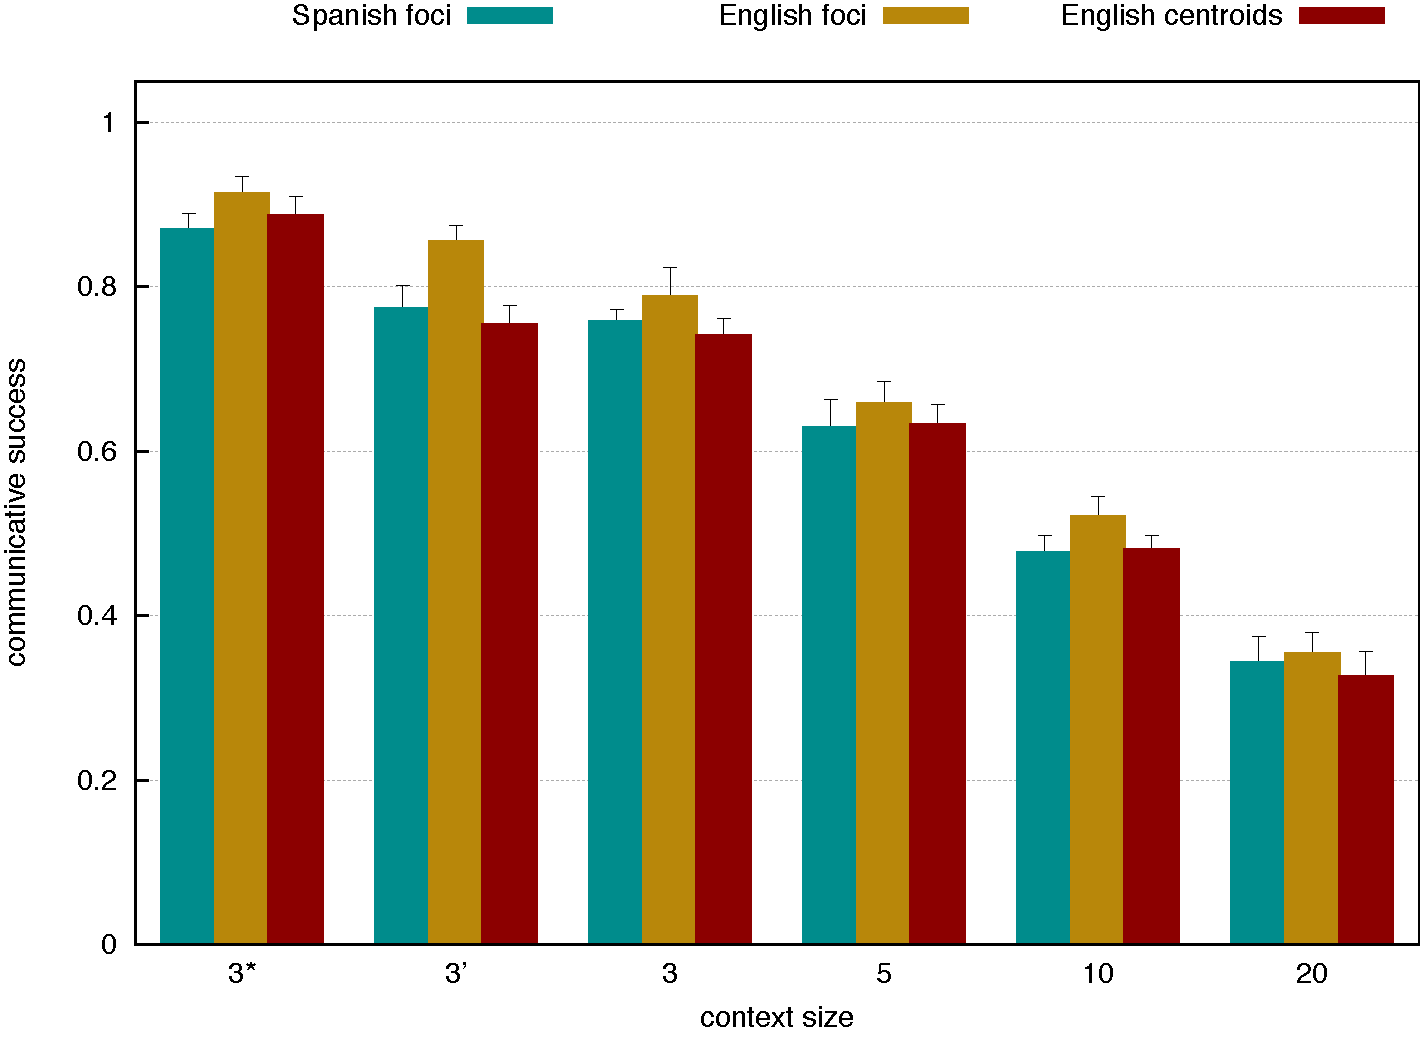
\includegraphics[width=.8\textwidth]{./basic-strategy/figures/baseline.pdf}
    \caption[The baseline communicative success of three predefined
    language systems]{The baseline communicative success of three
      predefined language systems: one is based on the Spanish foci
      \citep{lillo07locating} and the others are based on the foci and
      centroids of English \citep{sturges95location}. Baseline
      communicative success is inversely related to the context size
      increases. The context size for 3' is 3, but an additional
      constraint on the minimal interstimulus distance is
      imposed. Additionally, in 3* only the subset of Munsell chips
      that are faithfully reproducible are considered. These results
      are averaged over 8 runs.}
    \label{f:bcs-baseline}
  \end{center}
\end{figure}

The communicative success
\is{measures!communicative success}
\is{communicative success|see{measures}}
the ratio of
successful interactions in the last $cs_n$ games. The communicative
success has a maximum of 1 and minimum of 0. In all reported
experiments the value of $cs_n$ is set to 250.

\subsection{Results}

The communicative success of the baseline experiment is shown in
Figure \ref{f:bcs-baseline}. The more samples in one
context, the lower the corresponding communicative success. The
language system based on the English foci seems to perform slightly
better than the ones based on other language systems.


Imposing a minimal interstimulus distance of 50 in the CIE $L^*a^*b^*$
colour space (3' in Figure \ref{f:bcs-baseline}) does not
appear to have a significant impact on the resulting communicative
success, but the additional limitation to a particular subset of the
Munsell chip does (3* in Figure \ref{f:bcs-baseline}).

The main reason why some interactions still fail is that some samples
in a context could not be successfully discriminated because another
sample in the context was more similar to the prototype of the
category that the selected topic would belong to. For example, the
sample to the right in the context shown in Figure
\ref{f:bcs-failure-context}, will not be successfully named as
the middle sample is more similar to the prototype of the green colour
category.

\begin{figure}
  \begin{center}
    
\includegraphics[height=1.25cm]{./basic-strategy/figures/baseline-failure-context.pdf}
    \caption[Example context in which the basic colour strategy
    fails]{Example context in which the basic colour strategy
      fails. The sample to the right can not be successfully named as
      the middle sample is more similar to the prototype of the green
      colour category.}
    \label{f:bcs-failure-context}
  \end{center}
\end{figure}

\section{Conclusion}

In this chapter I have shown how the semantic and syntactic templates
of the basic colour strategy can be defined. I have proposed
semantics that builds upon previous research, both in psychology and
artificial language evolution, and have extended it to accommodate for
several substrategies in which some dimensions of the colour domain
are more relevant as accounted by documented language systems. I have
proposed a mapping to language that encodes these semantics.

\chapter{Graded Membership Strategy}
\label{s:graded-membership-strategy}
\is{language strategy!for colour!graded membership strategy}
\is{graded membership strategy|see{language strategy}}

Colour categories are assumed to be prototypical in nature
\citep{rosch73natural}, which implies that some colour samples are
better examples of a category than others. Some languages allow the
users to mark how well a particular sample represents the
prototype. In English this marking is optional and achieved through
the adverb ``very'' and the modifying ``-ish'' suffix, such as in the
expression ``greenish''. In Russian, the suffix ``-ato'' indicates a
similar meaning \citep{safuanova07russian}. In other languages, such
as Tarahumara, an indigenous language spoken in Northern Mexico, this
marking is obligatory. This language has an elaborate system of
modifiers that distinguishes three levels of membership: ``-kame''
which could be translated as ``very'', ``-name'' which could be
glossed as ``somewhat'' and ``-nanti'' for the lowest degree of
membership. An example of how this system is used for the Turahumara
colour category for red: ``Sit\'a-'' is shown in Figure
\ref{f:gms-burgress-tarahumara} \citep{burgress83tarahumara}.

\begin{figure}[htbp]
  \begin{center}
   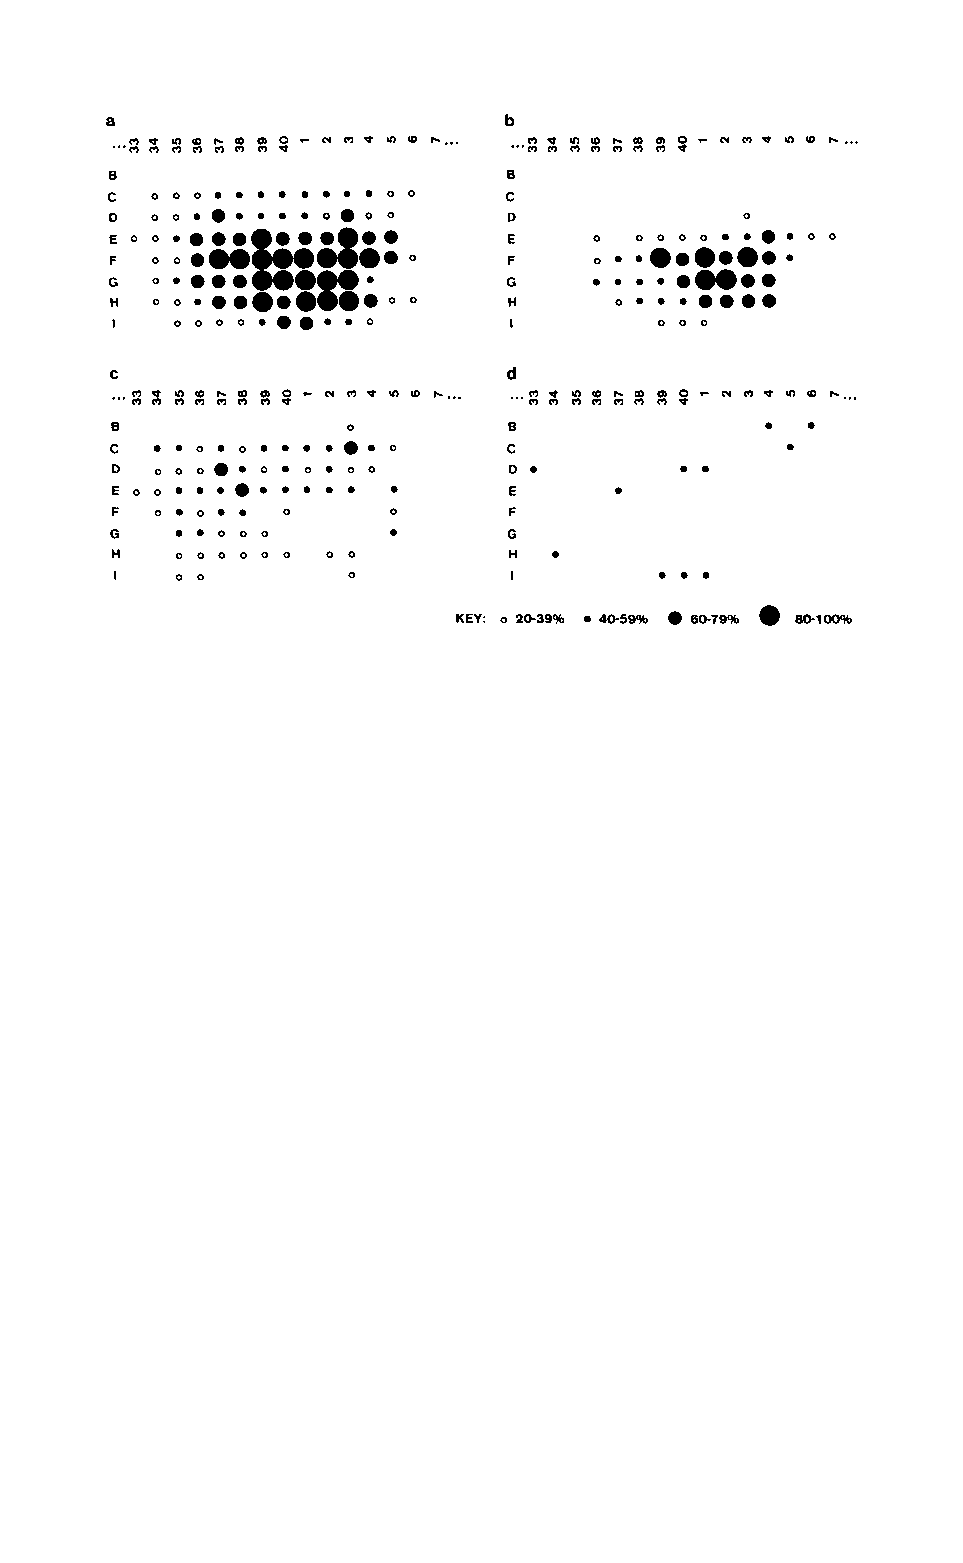
\includegraphics[width=\textwidth]{./graded-membership/figures/burgress-tarahumara.pdf}
   \caption[The use of modifiers in Tarahumara]{The use of modifiers
     to express graded membership in Tarahumara shown on the Munsell
     array. The bigger the circle, the more it represents a
     particular colour expression. (a) aggregate of all expressions
     using the ``Sit\'a'' root (b) ``Sit\'akame'' (very red) (c)
     ``Sit\'aname'' (somewhat red) (d) ``Sit\'ananti'' (only slightly
     red). Note how each modifier specifies a region that is further
     removed from the prototypical colour of ``Sit\'a''. Figure from
     \cite{burgress83tarahumara}.}
    \label{f:gms-burgress-tarahumara}
  \end{center}
\end{figure}

In this chapter, I will propose a compositional semantic template that
is capable of modelling these observations. I will also introduce the
grammatical syntactic templates that allow agents to express this
strategy in language. I will use Tarahumara as the main guiding
example.

\section{Related research}
\label{s:gms-related-research}

Although most models within artificial language evolution and colour
naming models represent the graded nature of membership of a colour
sample to a colour category, almost none of them deploy syntax to
express this membership. One exception is the colour naming model of
\citeauthor{mojsilovic02method}, which includes names for modifiers
and different lightness values \citep{mojsilovic02method,
  mojsilovic05computational}. The semantics of this model, however, is
quite limited as each compositional colour name is stored as a
different prototype based on a dictionary of colour names compiled by
the National Bureau of Standards \citep{kelly53icss}. It is unclear
how this model could be extended to allow for creative language use,
for example when names are not explicitly listed in the dictionary.

\section{Semantic template}
\label{s:gms-semantic-template}
\is{semantic template!for graded membership strategy}

Degree modifiers make the degree of membership of a particular entity
in the world to a category in the ontology of an agent explicit in
language. They split the continuous domain of membership into more or
less discrete categories. In order to propose semantics that capture
these observations, I need to make two choices: how the membership
function is computed and how the categorisation process based on this
membership function is implemented.

The membership function corresponds to the similarity function
introduced in Section \ref{s:bcs-categorisation}. The similarity of
the colour of an entity to a colour category maps directly on the
membership function: the more similar the colour of entity to the
prototype of the category, the higher the membership. The maximum
value of the membership function is one (when the colour of the entity
is exactly equal to the prototype of the category) and approaches zero
when they are very dissimilar.

The \emph{membership categories} are implemented as prototypical
categories. Each category has a prototypical value of the membership
and classification is organised following a standard nearest-neighbour
algorithm. Each entity is assigned to the membership category that is
most similar to it. Other approaches, such as discrimination trees
\citep{steels96perceptually}, could have been chosen, but the
prototype theory is sufficient to cover the main principles of the
\emph{graded membership strategy}.

This approach results in the definition of absolute ranges between a
colour sample and colour category due to the properties of the
membership function and how the membership categorisation process is
organised. The membership function is only dependent on the category
that is most similar to the sample and the membership categories are
defined as prototypical values of this membership function. As a net
result, a membership category defines an absolute range in distance
between the colour sample and the colour category. A schematic
representation of this approach is provided in Figure
\ref{f:gms-semantics-schematic}.

\begin{figure}[htbp]
  \centering
  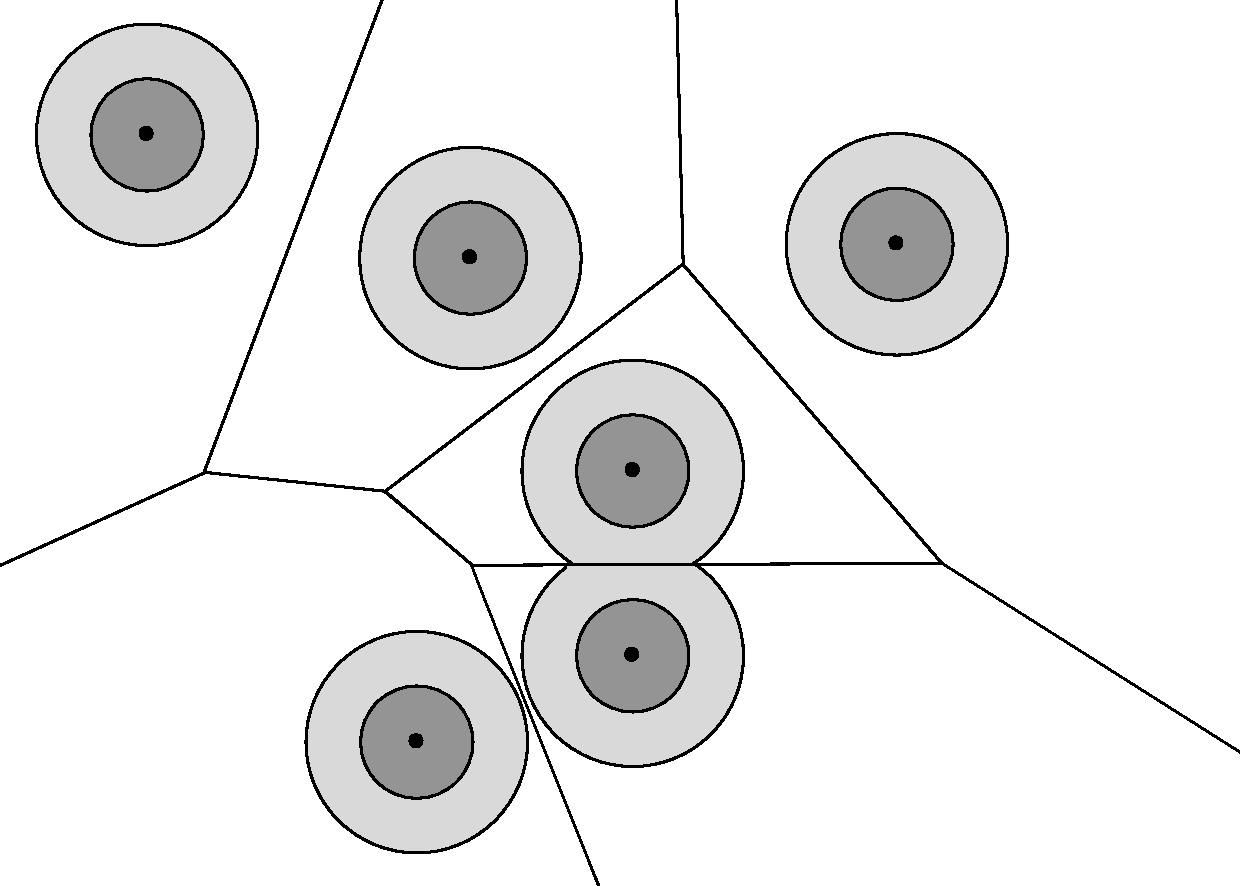
\includegraphics[width=.65\textwidth]{./graded-membership/figures/semantics-schematic.pdf}
  \caption[Schematic representation of the semantics of the graded
  membership strategy]{Schematic representation of the semantics of
    the graded membership. The categorisation based on colour
    categories results in a Voronoi tessellation of the conceptual
    space. The membership categories (marked in different shades of
    grey) define a fixed range starting from the prototype of the
    category.}
  \label{f:gms-semantics-schematic}
\end{figure}

The semantics of the \emph{graded membership strategy} can be
summarised as follows: first the entities are categorised as in the
\emph{basic colour strategy}. This process stores membership
information in the entities as a side-effect. Unlike the \emph{basic
  colour strategy}, not just the best member will be selected from
this set, but the resulting set will be categorised again based on the
membership information stored in the entities. This second
categorisation process changes the activation stored in the
entities. Selection will be based on this activation.

\subsection{Profiling and categorisation based on colour}

The categorisation process is similar to the one introduced for the
\emph{basic colour strategy}, except that this categorisation process
is now more strict. Even in interpretation, it assigns each entity to
the nearest known colour category. This is identical to the
categorisation during conceptualisation.

This modification is based on the observation that whenever the
\emph{graded membership strategy} is used, the base category will be
the category that is the most similar to the named sample. For
example, a sample that is named ``greenish'' is still more similar to
the prototype for green than to the prototype of brown.

Although strict interpretation is known to decrease the expected
communicative success when categories are not aligned between
individual language users \citep{belpaeme07language}, it ensures the
categorisation process applied by the speaker and hearer are
symmetrical. This is especially useful when processes become dependent
on each other. Asymmetrical processing might be another source of
potential communicative failures.

\subsection{Categorisation based on membership}

Each membership category is represented by its most prototypical
membership value. The membership value of each entity is compared to
the membership value stored in the category. Each entity is assigned
to the membership category that is most similar to it. More than one
entity can be categorised as the same category. This categorisation
process changes the activation in the entities.

\subsection{Selection based on activation}

This second categorisation process based on membership changes the
activation stored in the entities. The entity with the highest
activation will be selected as the outcome of the complete process.

\subsection{Semantic constraint network}

The semantic constraint network for the \emph{graded membership
  strategy} is shown in Figure \ref{f:gms-semantic-program}. The
\textsc{Equal-to-Context} and \textsc{Profile-Colour-Dimensions}
primitives are the same ones as introduced before. The
\textsc{Filter-by-Colour} primitive is similar to the
\textsc{Filter-by-Colour-Lenient} except that during interpretation it
applies a strict categorisation as well. The
\textsc{Filter-by-Membership} categorises the resulting sets based on
the membership information stored by the \textsc{Filter-by-Colour}
primitive. Finally, \textsc{Select-Most-Activated} selects the entity
with the highest activation.

\begin{figure}[htbp]
  \centering
  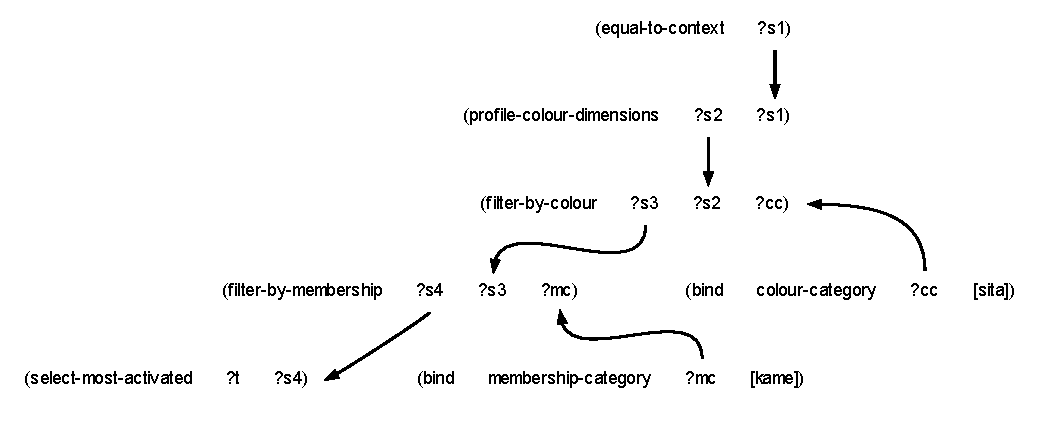
\includegraphics[width=\textwidth]{./graded-membership/figures/semantic-program.pdf}
  \caption[The semantic constraint network for the graded membership
  strategy]{The semantic constraint network for the graded membership
    strategy, which is similar to the one of the basic colour
    strategy. The \textsc{Filter-By-Membership} now categorises the
    resulting sets further. \textsc{Select-Most-Activated} selects the
    entity with the highest activation.}
  \label{f:gms-semantic-program}
\end{figure}

\subsection{Semantic primitives}

\definition{Semantic Primitive}{Filter-by-Colour}

\begin{explanation}{description}
  Categorises each entity in a source set as the most similar colour
  category known to the agent. The membership of each entity is set to
  be the the similarity to the category it belongs to.
\end{explanation}

\begin{explanation}{slots}
  \verb+?filtered-set+ (of type entity-set) \\
  \verb+?source-set+ (of type entity-set) \\
  \verb+?colour-category+ (of type colour-category)
\end{explanation}

\begin{explanation}{revision specs}
  \verb+?source-set+: categorises each entity of source set and
  returns pairwise bindings for the remaining slots; categories
  to which no entities are assigned, are ignored \\
  \verb+?source-set ?category+: computes the categorisation of the
  source set based on all colour categories known to the agent and
  when the resulting set for the provided colour category is not
  empty, it gets bound to \verb+?filtered-set+
\end{explanation}

\definition{Semantic Primitive}{Filter-by-Membership}

\begin{explanation}{description}
  Categorises each entity in a source set as the most similar
  membership category known to the agent.
\end{explanation}

\begin{explanation}{arguments}
  \verb+?filtered-set+ (of type entity-set) \\
  \verb+?source-set+ (of type entity-set) \\
  \verb+?membership-category+ (of type membership-category)
\end{explanation}

\begin{explanation}{revision specs}
  \verb+?source-set+: categorises each entity in the source set as one
  of the known membership categories and returns pair-wise bindings
  for \verb+membership-category+ and \verb+?filtered-set+ \\
  \verb+?source-set ?membership-category+: computes the categorisation
  of the source set based on all membership categories known to the
  agent and when the resulting set for the provided membership category
  is not empty, it gets bound to \verb+?filtered-set+
\end{explanation}

% \definition{Semantic Primitive}{Select-Unique-Element}

% \begin{explanation}{description}
%   Checks whether an entity set contains only one element and binds it
%   to the other slot.
% \end{explanation}

% \begin{explanation}{slots}
%   \verb+?entity+ (of type colour-entity) \\
%   \verb+?entity-set+ (of type entity-set)
% \end{explanation}

% \begin{explanation}{revision specs}
%   \verb+?entity-set+: when the entity-set is a singleton, binds
%   \verb+?entity+ to its sole member
% \end{explanation}

\subsection{Alternative approaches to semantics}

Several alternative approaches to the proposed semantics exist. One
alternative that has been used in previous models is to model basic
colour categories as one or more multidimensional `normalised'
Gaussian functions \citep{lammens94computational,
  steels05coordinating}. The similarity measure between a colour
category and a colour sample is weighted by the inverse of the
standard deviation in each dimension. This distance measure is also
known as the Mahalanobis distance.

It might be tempting to model graded membership by modifying the
standard deviation of a category: intensifiers such as ``very'' could
be implemented as decreasing the standard deviation and diminutives
like ``slightly'', could increase the standard deviation. This
corresponds to the idea that intensified categories should be
interpreted more strictly, which is reflected by a lower standard
deviation. This however leads to the unwanted outcome that the
diminutive will always be preferred among the three variants
(intensifier, diminutive and unmodified) as it results in the lowest
distance and hence the highest similarity to a particular colour
sample. This is due to the Mahalanobis measure which divides the
distance in each dimension by its standard deviation. The higher the
standard deviation, the lower the distance. A different similarity or
distance function would be needed to extend this approach to
modifiers.

Another approach that has often been pursued for modelling categories
is based on the fuzzy set theory \citep{kay78linguistic,
  benavente08parametric}. Some features of language, including
modifiers, have been studied using this approach
\citep{hersh76fuzzy}. These studies suggested that the probability of
the membership of an intensified category is a power of the membership
of the unintensified category. This again reflects the intuitive idea
that membership to an intensified category should decrease faster than
membership to the original category, but fails to account for why
intensified categories should be favoured over orginal categories for
the best members of the fuzzy set.

\section{Syntactic templates}
\label{s:gms-syntactic-templates}

The templates to express this network in language are in general
similar to the one used for the \emph{basic colour strategy} in
Section \ref{s:bcs-syntactic-templates}: the semantic network is
divided in three layers of units: (a) entity units containing the
semantic entities, (b) functional units which make direct use of such
a semantic entity and (c) contextual units which contain any remaining
operations of the semantic constraint network that do not make direct
use of any semantic entity. The main difference is that in order to
express both the \emph{basic colour strategy} and the \emph{graded
  membership strategy}, an additional template can be used to allow
the re-use of the contextual rule introduced for the basic colour
strategy.

The linguistic structure for ``sita-kame'' is shown in Figure
\ref{f:gms-linguistic-structure}. Besides introducing the colour
category for ``sita'', the lexicon rules now also introduce the
membership category for ``kame''. Functional rules take care of the
\textsc{Filter-by-Colour} and \textsc{Filter-by-Membership}
primitives. All other parts of the semantic network are grouped in a
contextual rule, which also ensures that the two functional primitives are
linked into the other primitives of the network.

\begin{figure}[htbp]
  \centering
  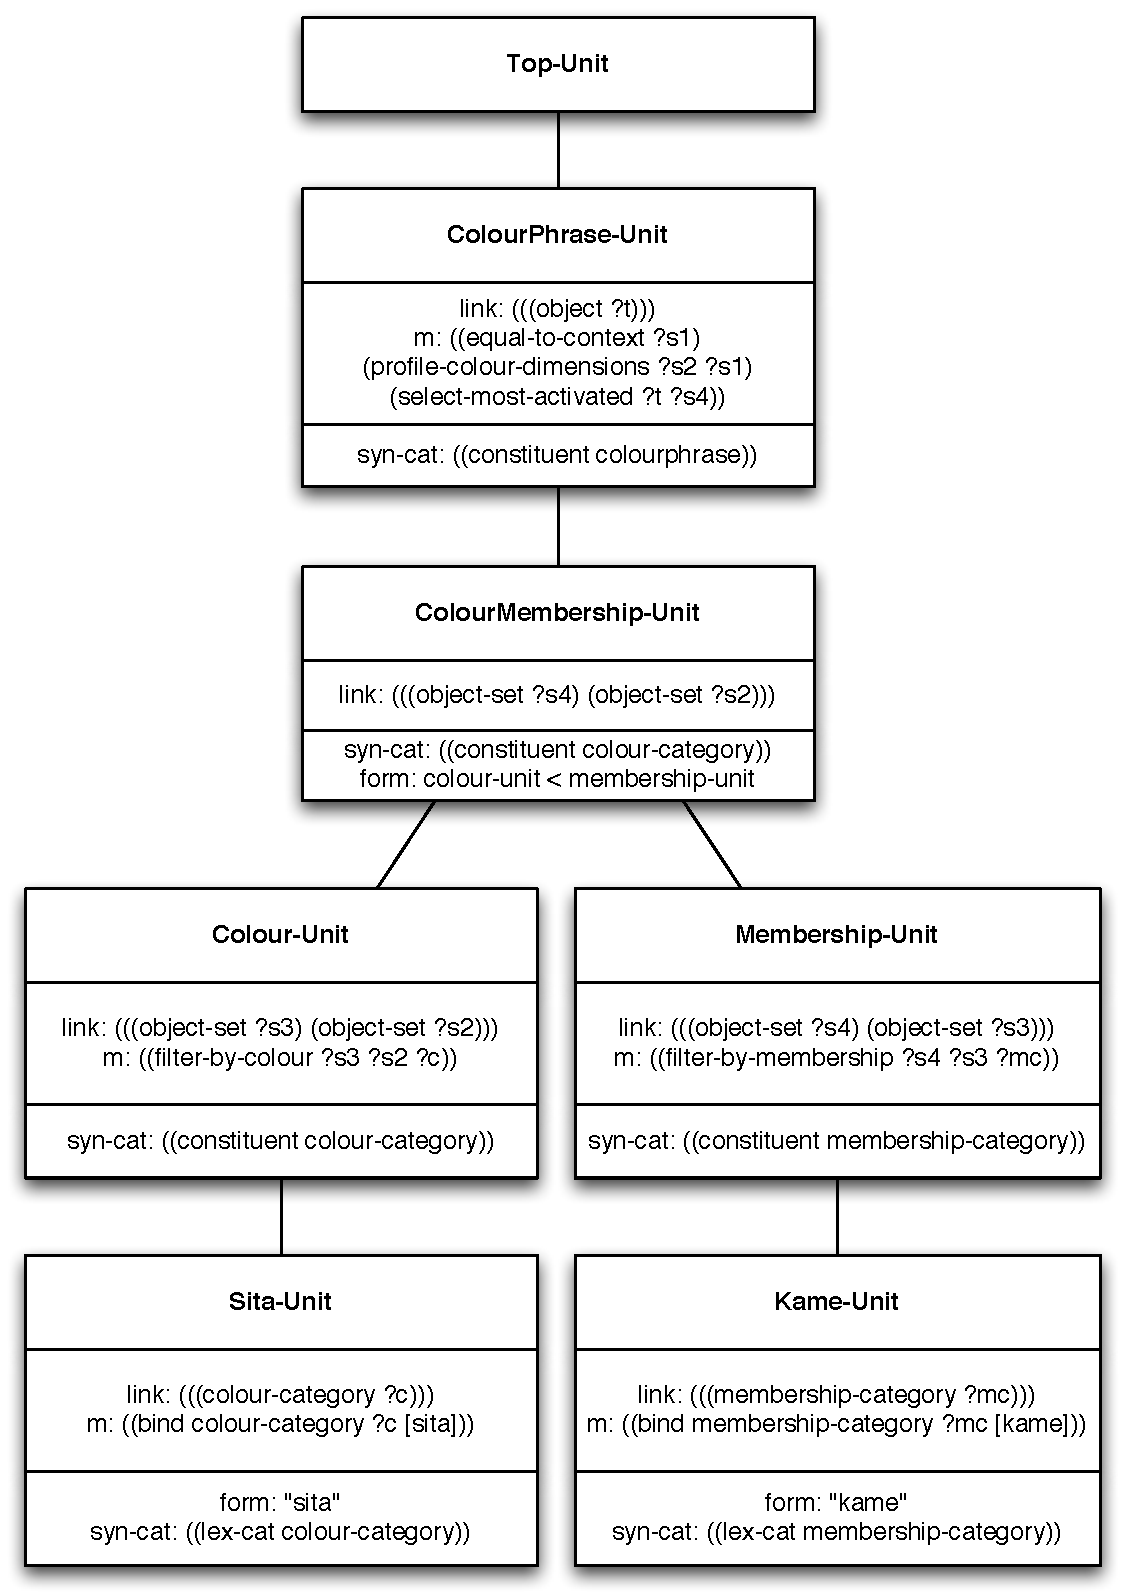
\includegraphics[width=.85\textwidth]{./graded-membership/figures/linguistic-structure.pdf}
  \caption[Linguistic structure for graded membership
  strategy]{Linguistic structure for graded membership strategy. Both
    semantic and syntactic poles are shown in the same
    structure. Semantic information is shown in the top part of each
    unit, the syntactic information in the bottom part of each
    unit. The structure consists of four layers: one for the semantic
    entities, one for the functional primitives and the top one
    represents the contextual rule introduced in the previous
    chapter. The additional ColourMembership-Unit is introduced by a
    rule based on Syntactic template 2.}
  \label{f:gms-linguistic-structure}
\end{figure}

\subsection{Syntactic template 1.1: Semantic entities}
\is{syntactic template!for semantic entities}

The entity rules for membership categories are very similar to the one
I introduced in the previous chapter for colour categories. During
parsing it will introduce the membership category. In production, it
will introduce the string that is associated with this category. In
both modes a new unit is introduced that encapsulates this
information. On the semantic side, the \emph{link} feature
will allow
other rules to incorporate the membership category in the semantic
network during parsing.

\footnotesize
\begin{Verbatim}[frame=lines, label=Entity rule for kame]
((?top-unit
  (tag ?meaning 
       (meaning ((bind membership-category ?c [kame])))))
 ((J ?kame-unit ?top-unit)
  ?meaning
  (link (((membership-category ?mc))))))
<-->
((?top-unit
  (tag ?form 
       (form ((string ?yellow-unit "kame")))))
 ((J ?kame-unit ?top-unit)
  ?form
  (syn-cat ((lex-cat membership-category)))))
\end{Verbatim}
\normalsize

\subsection{Syntactic template 1.2: Functional primitives}
\is{syntactic template!for functional primitives}

The functional rules for \textsc{Filter-by-Colour} and
\textsc{Filter-by-Membership} are similar to the functional rule for 
\textsc{Filter-by-Colour-Lenient} in the previous chapter. An example
of such a rule for \textsc{Filter-by-Membership} is shown below.

\footnotesize
\begin{Verbatim}[frame=lines, label=Functional rule for Filter-by-Membership]
((?top-unit
  (sem-subunits (?membership-category-unit)) 
  (tag ?meaning
       (meaning ((filter-by-membership ?s4 ?s3 ?mc)))))
 (?membership-category-unit 
  (link (((membership-category ?c)))))
 ((J ?filter-by-membership-unit ?top-unit 
      (?membership-category-unit))
  ?meaning
  (link (((entity-set ?s4) (entity-set ?s3))))))
<-->
((?top-unit 
  (syn-subunits (?membership-category-unit)))
 (?membership-category-unit 
  (syn-cat ((lex-cat membership-category))))
 ((J ?filter-by-membership-unit ?top-unit 
      (?membership-category-unit))
  (syn-cat ((constituent membership-category)))))
\end{Verbatim}
\normalsize

\subsection{Syntactic template 2.1: Re-use of constructions}
\is{syntactic template!re-use of constructions}

Re-use also occurs when the agent already knows a construction which
covers part of the meaning to be conveyed. Such a template fix the
glitches that prevent other rules to apply. Let us consider the
situation in which an agent needs to be able to express both the
\emph{strict basic colour strategy} and the \emph{graded membership
  strategy}. The strict basic colour strategy is identical to the
normal basic colour strategy, except that it uses
\textsc{Filter-by-Colour} primitive instead of a
\textsc{Filter-by-Colour-Lenient} primitive for categorisation.  The
semantic templates of both strategies share the same contextual
primitives, so re-use of the same contextual rule could be achieved. In
order to do so, a new unit needs to be introduced to the structure
that combines two subunits into one and that also takes care of
variable equalities between the subunits and contextual rule. An
example of such a `glue'-rule is shown below. This rule allows the
agents to re-use the contextual rule for the \emph{basic colour
  strategy} to express the \emph{graded membership strategy}.

\footnotesize
\begin{Verbatim}[frame=lines, label=ColourMembership rule]
((?top-unit 
  (sem-subunits (?membership-unit ?colour-unit)))
 (?membership-unit 
  (link (((entity-set ?s4) (entity-set ?s3)))))
 (?colour-unit 
  (link (((entity-set ?s3) (entity-set ?s2)))))
 ((J ?colourmembership-unit ?top-unit 
      (?membership-unit ?colour-unit))
  (link (((entity-set ?s4) (entity-set ?s2))))))
<-->
((?top-unit
  (syn-subunits (?membership-unit ?colour-unit))
  (tag ?form 
       (form ((meets ?colour-unit ?membership-unit)))))
 (?membership-unit
  (syn-cat ((constituent membership-category))))
 (?colour-unit 
  (syn-cat ((constituent colour-category))))
 ((J ?colourmembership-unit ?top-unit 
       (?membership-unit ?colour-unit))
  ?form
  (syn-cat ((constituent colour-category)))))
\end{Verbatim}
\normalsize


\section{Baseline experiment}
\label{s:gms-baseline-experiment}
\is{baseline experiment!for graded membership strategy}

In the baseline experiment, I will compare three different predefined language
systems: the first two will only be able to categorise based on the
basic colour categories, while the third language will additionally be
able to express the degree of membership in language through
modifiers.

The first two language systems are based on English
\citep{sturges95location} and Central Tarahumara
\citep{burgress83tarahumara}. Although in Tarahumara the use of
modifiers is obligatory to express a colour sensation, the artificial
language system in which they are not allowed to do so will allow me
to assess the actual impact of the categorisation based on membership
and to assess the impact of the number of basic colour categories on
the resulting communicative success. English has 11 basic colour
categories, whereas Tarahumara only has 5 \citep{kay08number}.

As the exact location of the basic colour categories in Tarahumara are
not readily available in literature, I have made an estimation
based on the data reported in the World Color Survey
\citep{kay10world}. More than 5 colours terms have been reported for
Tarahumara in this study, from which I have selected the 5 most common
ones as being the basic colour terms. In these data, the foci
indicated by each informant are noted as chips indicated on the
Munsell array. The Munsell chip that was indicated by the highest
number of the 9 informants was selected as the focus of that
category. An overview of the resulting category system can be found in
Figure \ref{f:gms-tarahumara-basic}.

\begin{figure}[htpb]
  \centering
  
\includegraphics[width=.6\textwidth]{./graded-membership/figures/tarahumara-basic-categories.pdf}
  \caption[The basic colour categories for Central Tarahumara]{The
    basic colour categories for Central Tarahumara. These are the
    estimated foci of each category based on data from the World Color
    Survey \citep{kay10world}. From left to right (including the
    corresponding Munsell chip): ``ros\'a'' (7.5R 9 2), ``ch\'o''
    (5.0R 2 8), ``sit\'a'' (5.0R 5 14), ``siy\'o'' (2.5BG 4 8) and
    ``sawar\'o'' (5.0YR 7 14).}
  \label{f:gms-tarahumara-basic}
\end{figure}

As no exact data for the modifiers in Tarahumara are available, I have
estimated their prototypical membership values in such a way that each
of them cover a reasonable number of colour chips (560 for ``-kame'',
1445 for ``-name'' and 643 for ``-nanti''). Due to the absolute
nature of the membership categories, the proportion of the chips that
will be classified as each membership category depends on the colour
category they modify and its surrounding colour categories. The actual
prototypical values are provided in Table
\ref{t:gms-tarahumara-modifiers}.

\begin{table}[htpb]
  \centering
  \begin{tabular}{cd{4}}
  \lsptoprule
    membership category & \multicolumn{1}{c}{prototypical value}\\
    \midrule
    \itshape -kame & 0.2 \\
    \itshape -name & 0.02 \\
    \itshape -nanti & 0.002\\
    \lspbottomrule
  \end{tabular}
  \caption[Membership categories for Central Tarahumara]{Membership
    categories for Central Tarahumara. The higher the prototypical
    value, the more similar the colour category and the colour sample
    have to be.}
  \label{t:gms-tarahumara-modifiers}
\end{table}

A first test whether the proposed membership categories are valid is
provided by a naming benchmark\is{naming benchmark!for graded
  membership strategy}. This benchmark involves naming each of the
Munsell chips and grouping the samples based on the resulting
name. The results for two roots, ``sit\'a'' and ``sawar\'o'' are shown
in Figure \ref{f:gms-baseline-sita-sawaro}. In this figure, the
samples for one root are separated in more or less equal parts using
the three modifiers. These results are qualitatively similar to the
reported use of modifiers in Tamahumara as shown in Figure
\ref{f:gms-burgress-tarahumara}.

\begin{figure}[htbp]
\centering
\subfigure{
  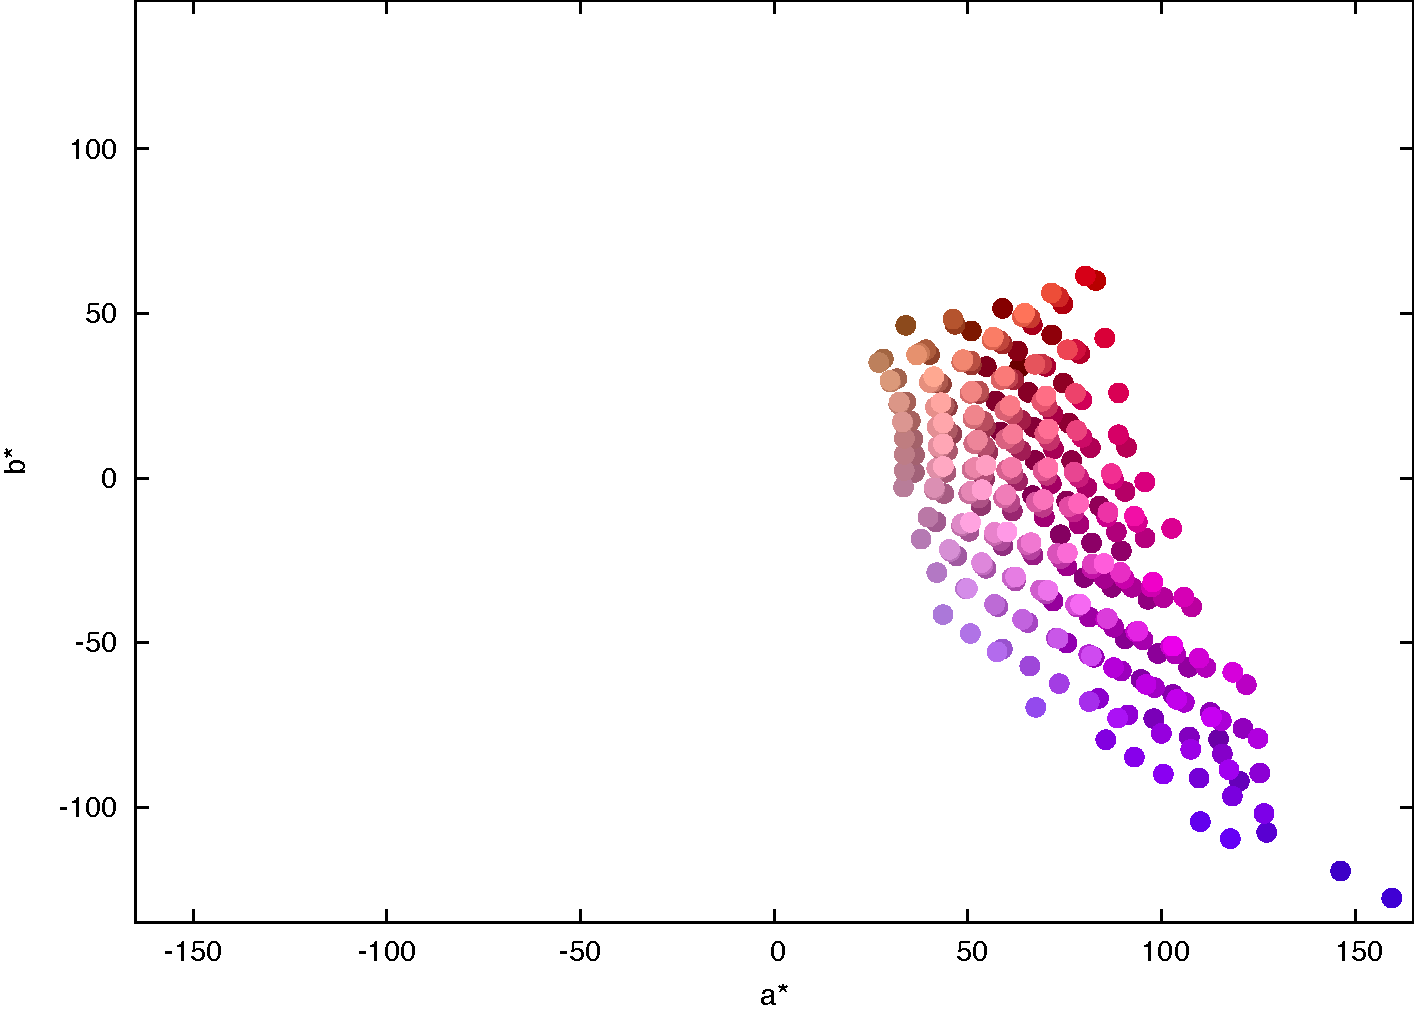
\includegraphics[width=.4\textwidth]{./graded-membership/figures/sita.pdf}
}
\subfigure{
  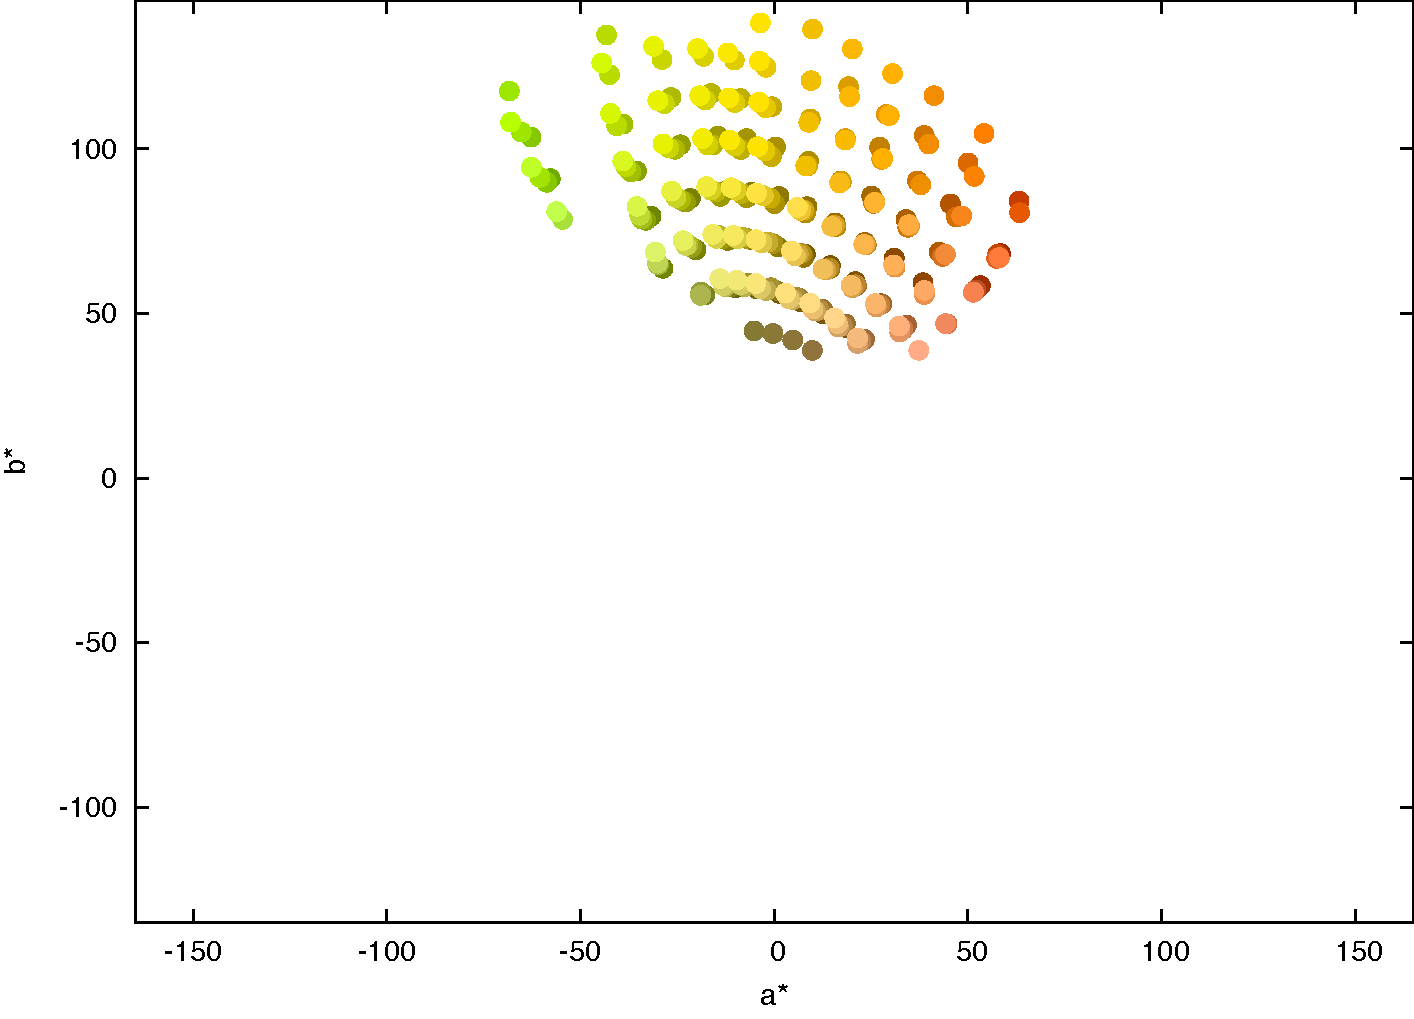
\includegraphics[width=.4\textwidth]{./graded-membership/figures/sawaro.pdf}
}
\subfigure{
  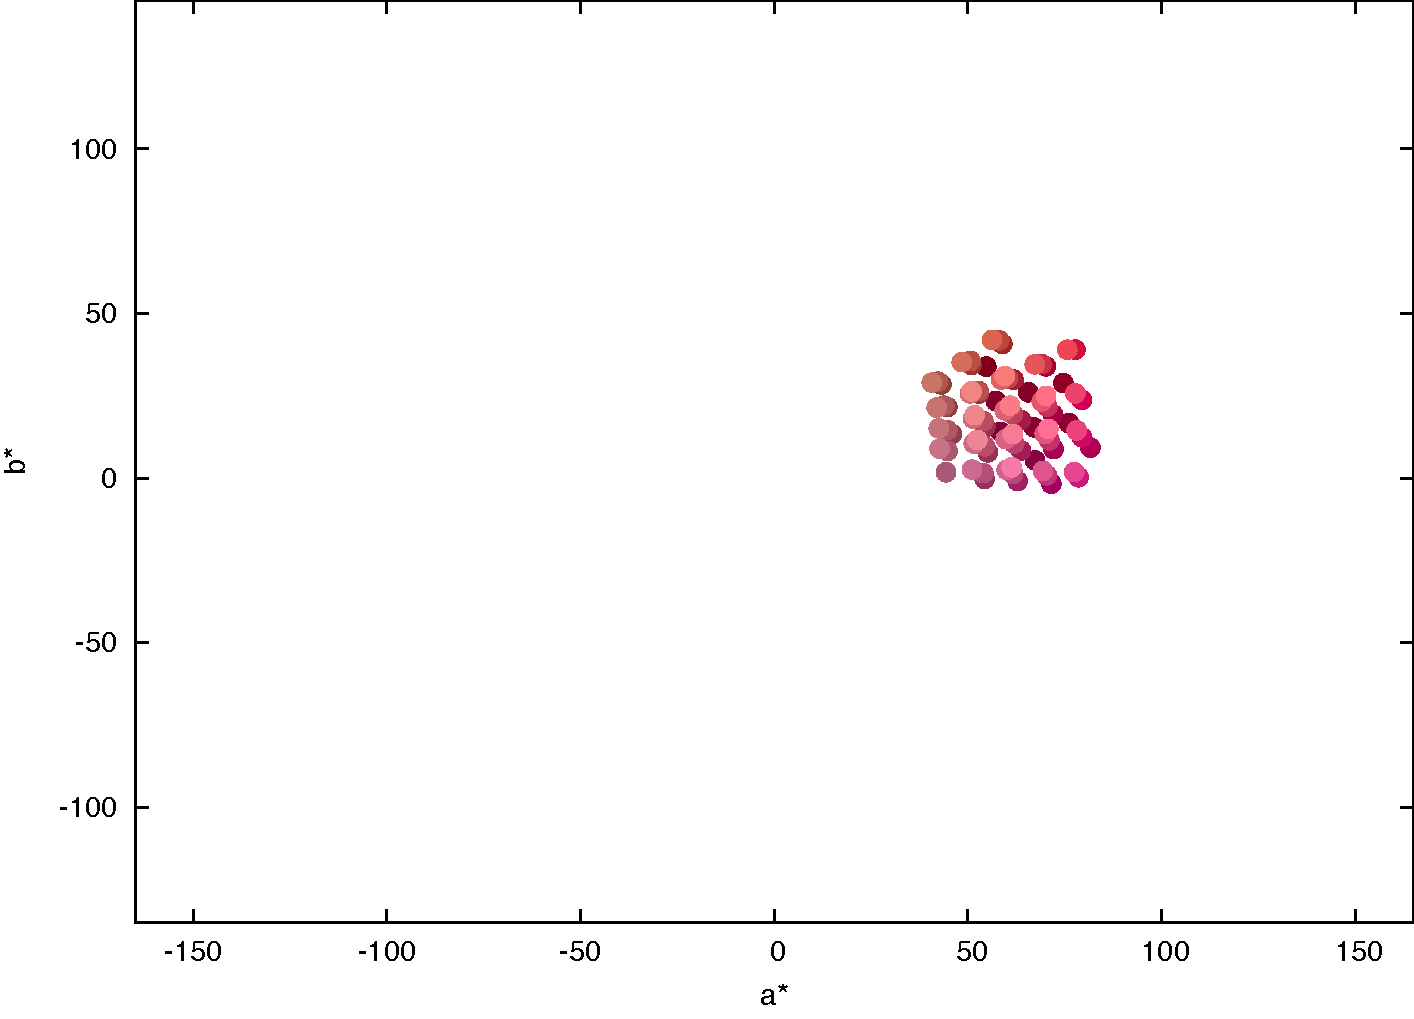
\includegraphics[width=.4\textwidth]{./graded-membership/figures/sita-kame.pdf}
}
\subfigure{
  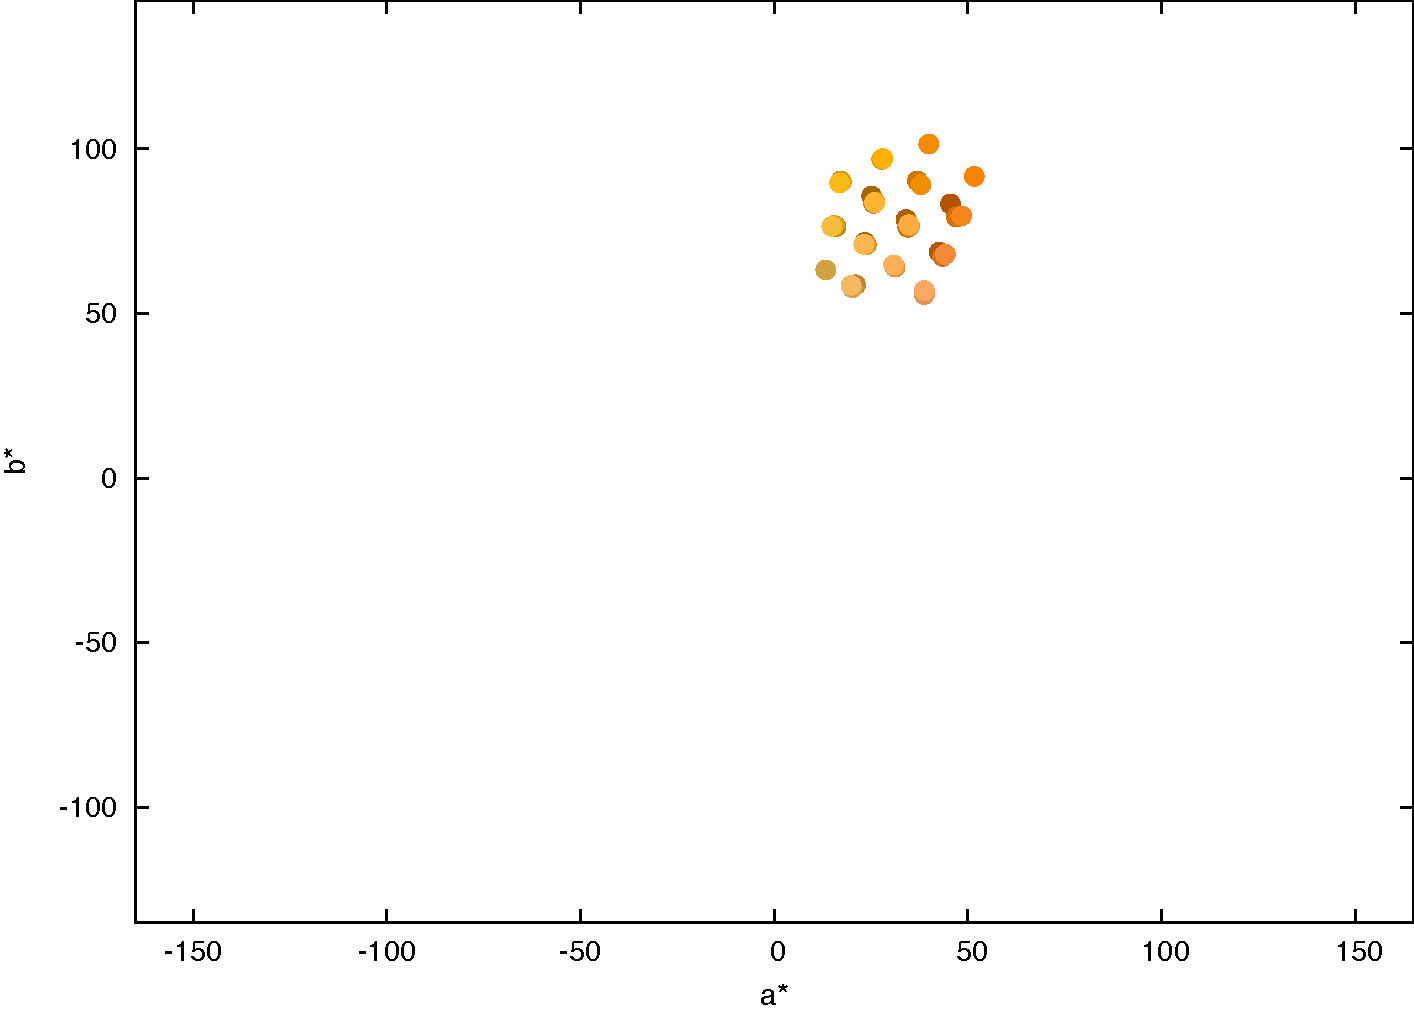
\includegraphics[width=.4\textwidth]{./graded-membership/figures/sawaro-kame.pdf}
}
\subfigure{
  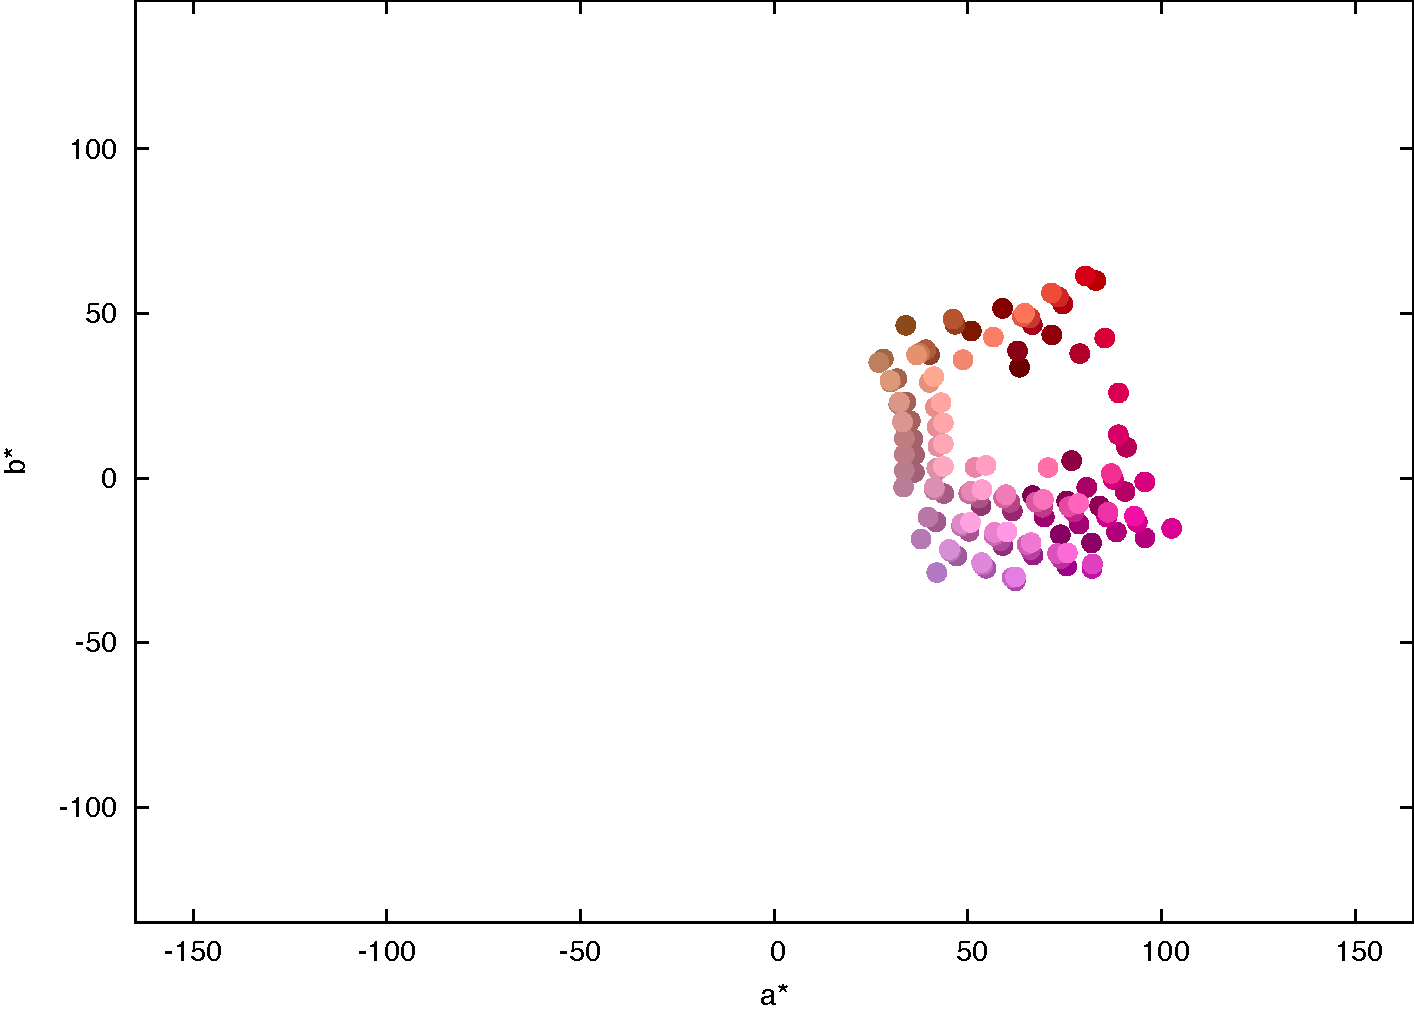
\includegraphics[width=.4\textwidth]{./graded-membership/figures/sita-name.pdf}
}
\subfigure{
  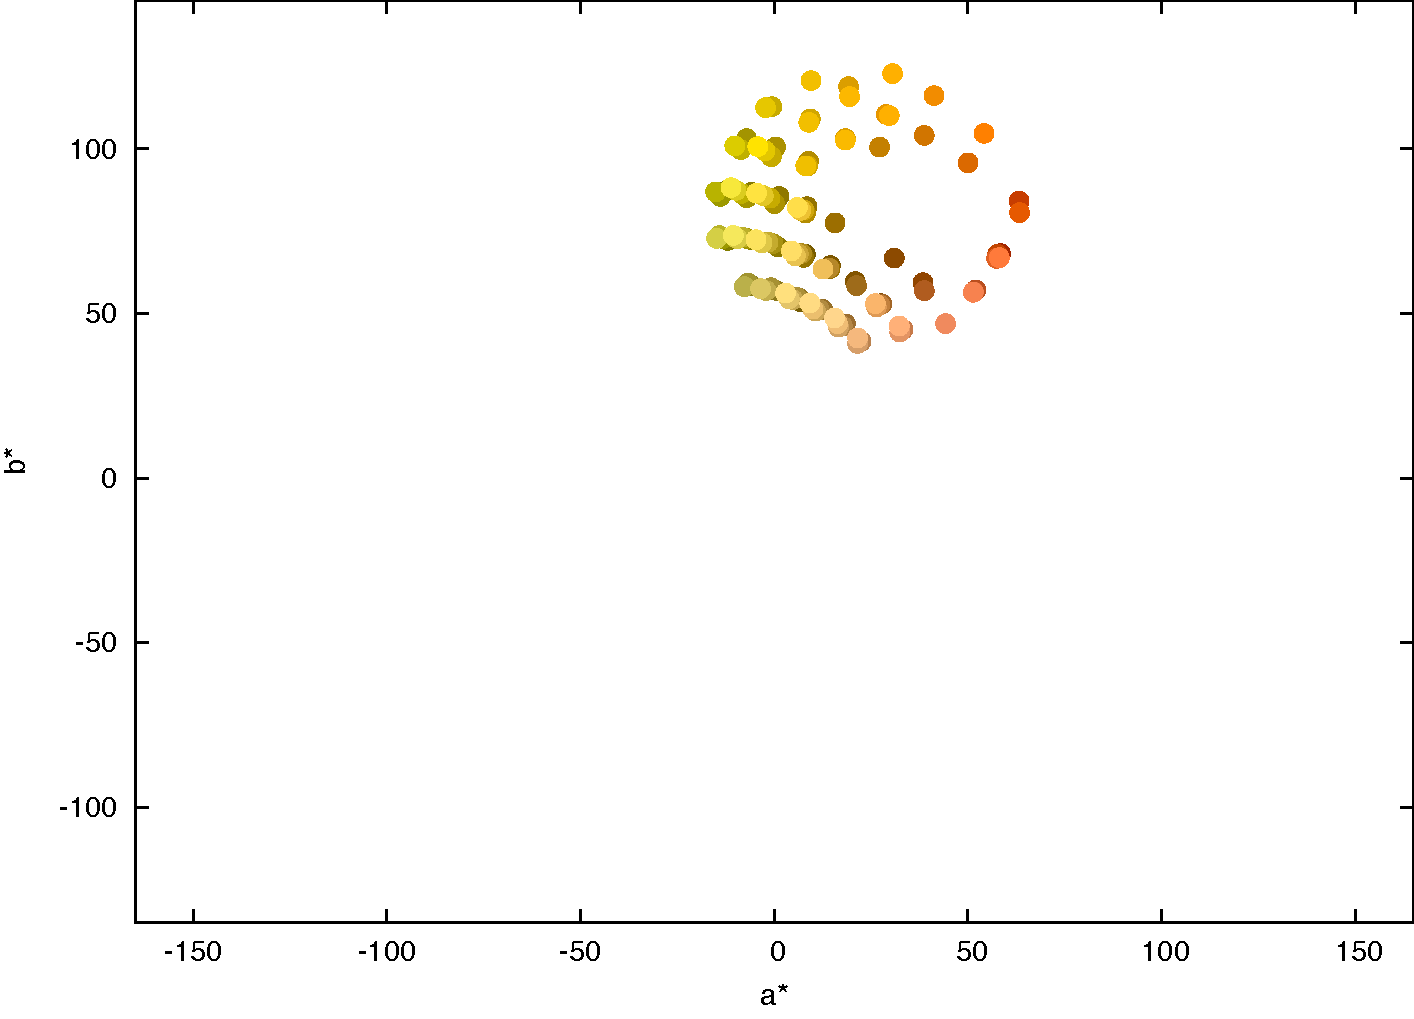
\includegraphics[width=.4\textwidth]{./graded-membership/figures/sawaro-name.pdf}
}
\subfigure{
  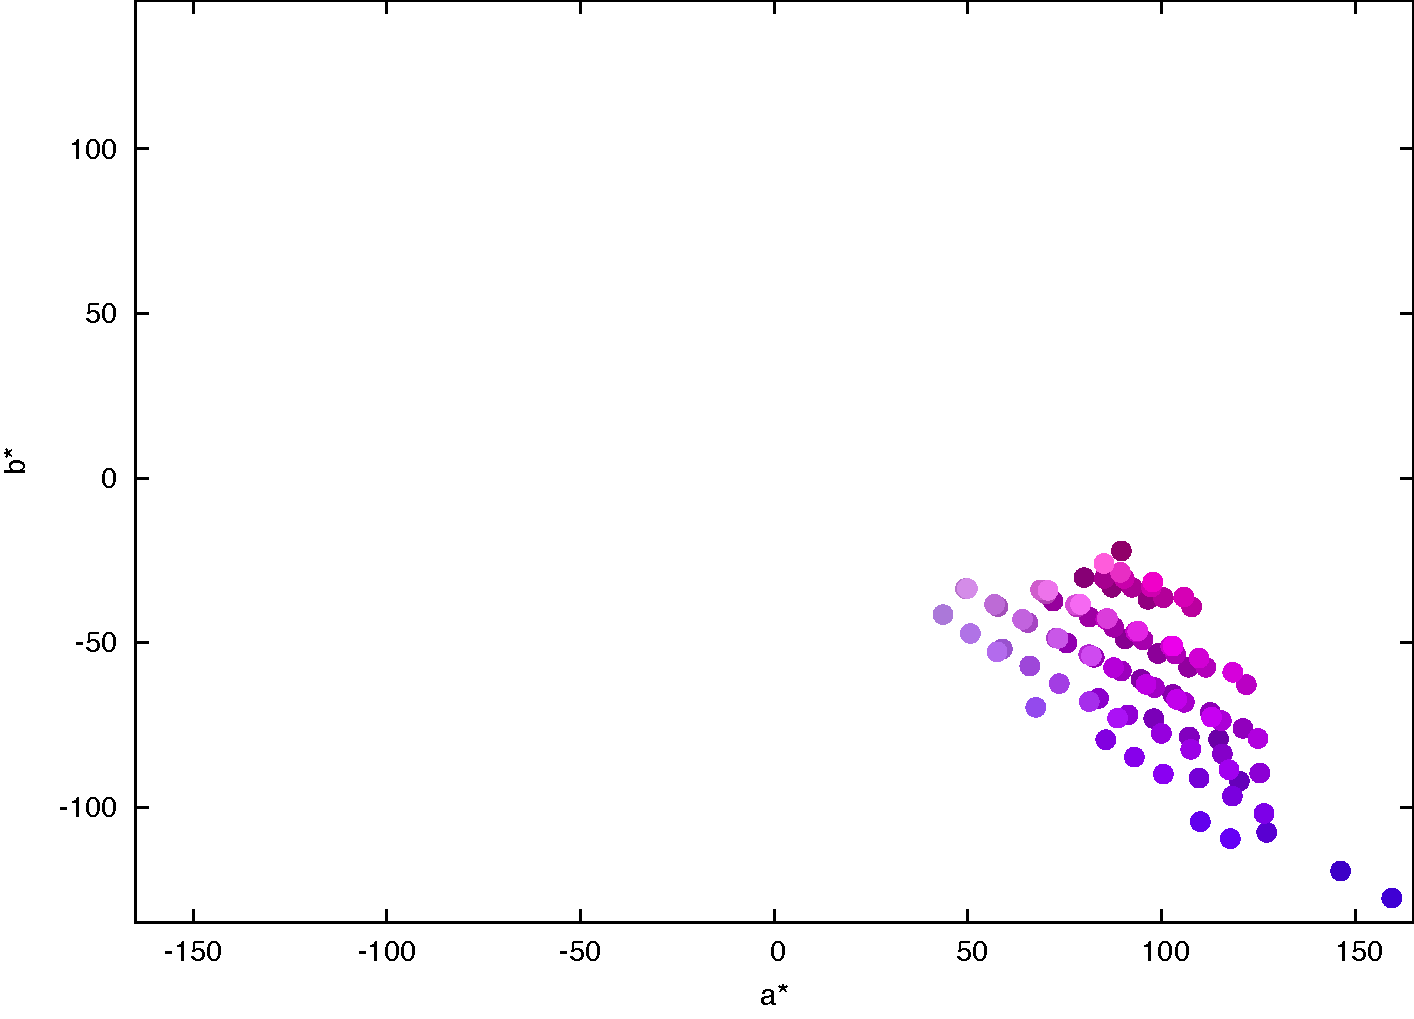
\includegraphics[width=.4\textwidth]{./graded-membership/figures/sita-nanti.pdf}
}
\subfigure{
  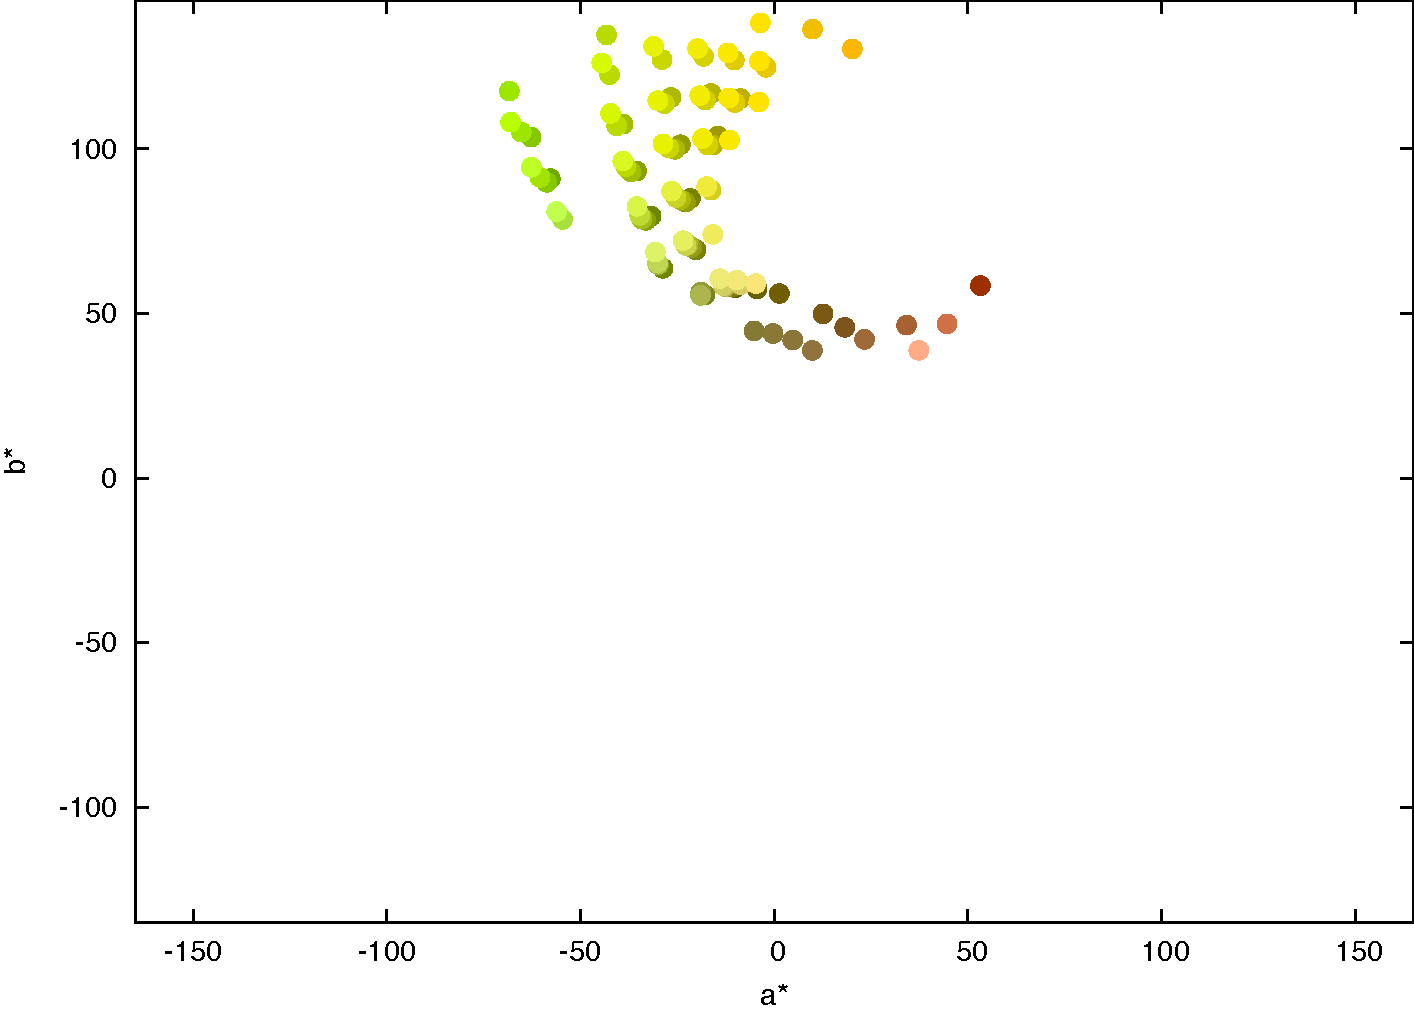
\includegraphics[width=.4\textwidth]{./graded-membership/figures/sawaro-nanti.pdf}
}
\caption[Example of modelled graded membership for Tarahumara]{Example
  of modelled graded membership for ``sit\'a'' (left) and ``sawar\'o''
  (right) in Tamahumara. The top row shows the aggregate of all uses
  of the corresponding term as root , the second row the uses of the
  \mbox{``-kame''} (very) modifier, the third row the uses of ``-name''
  (somewhat) and the bottom row show the uses of ``-nanti'' (only
  slightly). All diagrams are projections on the hue plane of the CIE
  $L^*a^*b^*$ colour space.}
\label{f:gms-baseline-sita-sawaro}
\end{figure}

\begin{figure}[p]
  \centering
  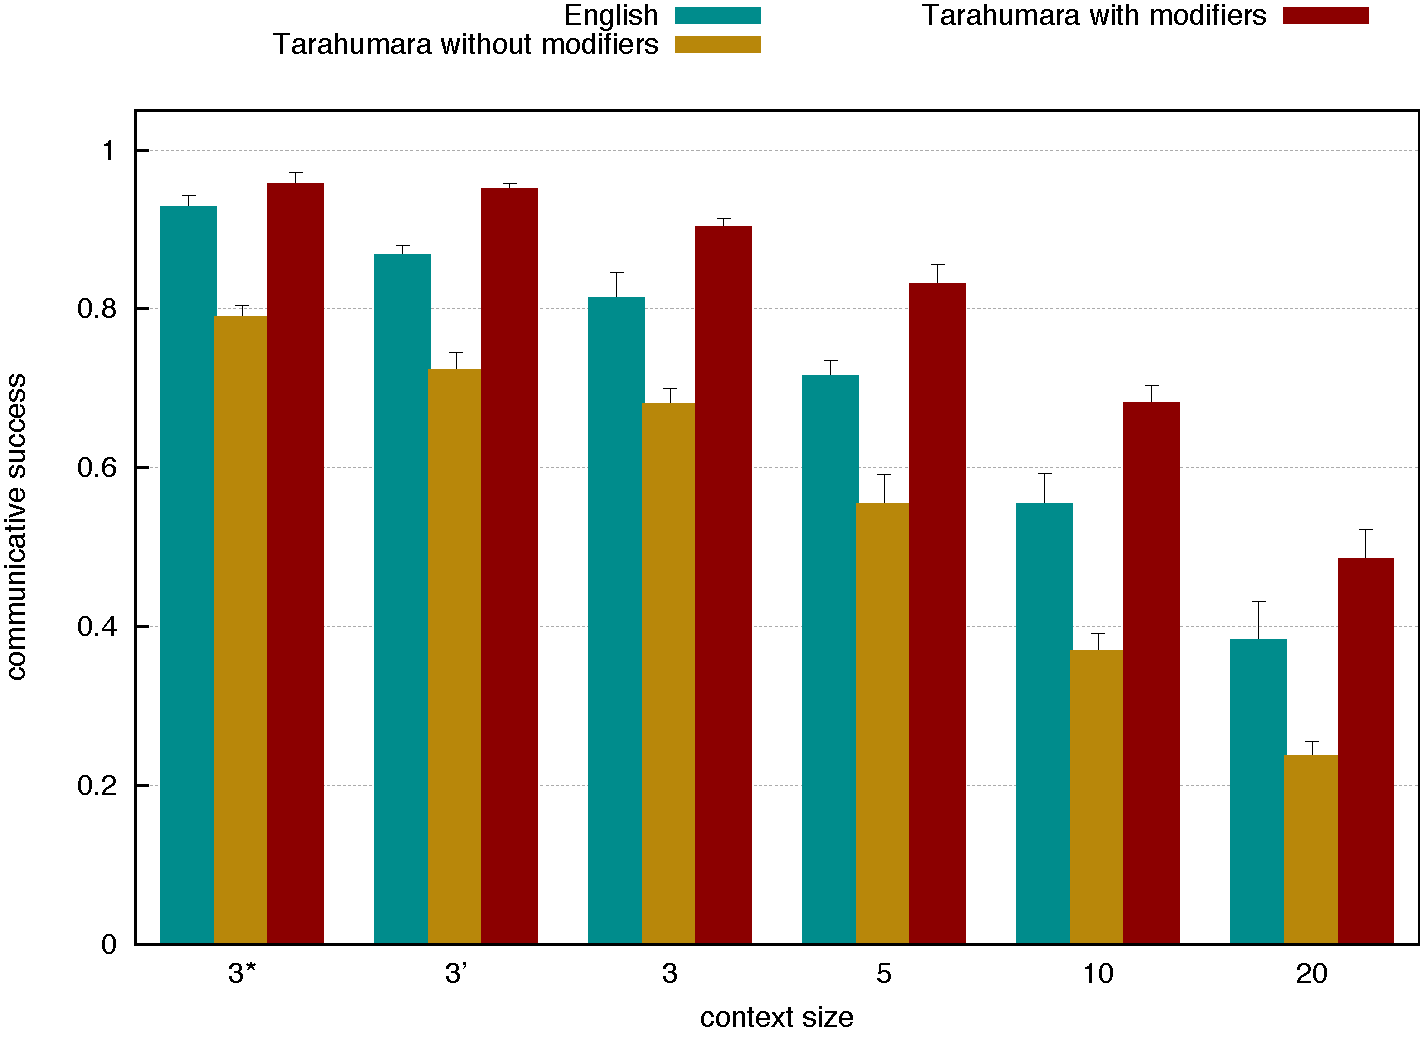
\includegraphics[width=\textwidth]{./graded-membership/figures/baseline.pdf}
  \caption[The baseline communicative success for graded membership
  strategy]{The baseline communicative success for graded membership
    strategy, comparing three different language systems: two are
    limited to the basic colour strategy and are based on English (11
    terms) and Tarahumara (5 terms). The third system is based on
    Tarahumara as well, but involves the graded strategy using 3
    modifiers. The lower number of basic terms has a negative impact
    on communicative success, but this can be overcome by allowing the
    use of modifiers.}
  \label{f:gms-baseline}
\end{figure}

\subsection{Results}
\label{s:gms-baseline-results}

The resulting communicative success of the baseline experiment is
shown in Figure \ref{f:gms-baseline}. A lower number of basic
categories has a negative impact on the communicative success (compare
English to Tarahumara without modifiers) but this effect can be
countered by allowing the use of modifiers (compare Tarahumara with
and without modifiers). Most interestingly, by allowing the use of
modifiers a system with a lower number of basic categories can become
more expressive than systems with a higher number of basic categories
that does not allow for modifiers (compare Tarahumara with modifiers
and English).

In systems in which only the strict basic strategy is deployed, the
chosen sample needs to be discriminable by one category which is
enforced by the selection process. The higher the number of
categories, the lower the chance another sample will be categorised as
the category of the topic. This explains the first observation that a
lower number of basic categories results in a lower baseline
communicative success.

When modifiers are allowed in the language system, the restriction of
a single discriminatory category is somewhat loosened. Instead of a
single category to be discriminative, it now is the consecutive
filtering using a colour category and a membership category that needs
to be discriminative. This explains why allowing modifiers has a
positive impact on the resulting baseline success.


\section{Conclusion}

In this chapter, I have introduced a compositional semantics for the
\emph{graded membership strategy} and linguistic rules to express the
membership categories in language. I have qualitatively compared the
resulting names to those reported for the Tarahumara language using a
naming benchmark. I have also shown the positive impact of the use of
modifiers on the baseline communicative success, which can counter the
negative impact of a lower number of basic colour categories.
\chapter{Category combination strategy}
\label{s:category-combination-strategy}
\is{language strategy!for colour!category combination strategy}
\is{category combination strategy|see{language strategy}}

Some languages also allow users to compound two colour categories into
a new one. This can also be applied to the domain of colour,
especially to describe a colour sample that is not a good example of
any of the basic colour terms.  An example in English would be
\textit{blue-green}. This compounding can also be modulated by an
additional marker, like for example \textit{-ish} in English as in
\textit{brownish-red}. Other languages, such as Vietnamese, allow to repeat
one colour term to give it emphasis, as in \textit{yellow yellow}
\citep{alvarado02modifying}.

\cite{safuanova07russian} have collected data on the focal colours of
compounds in Russian. One of their main findings is that in Russian,
the order in which colour terms are combined has an influence on the
resulting focal colour: the second term seems to be more important in
the expression. This is illustrated in Figure \ref{f:ccs-russian}. The
colours between \textit{\v z\"eltyj} (`yellow') and \textit{zel\"eno} (`green') are
for example named: \textit{zelenovato-\v z\"eltyj} (`greenish-yellow'),
\textit{zel\"eno-\v z\"eltyj} (`green-yellow'), \textit{\v z\"elto-zel\"enyj}
(`yellow-green') and \textit{\v z\"eltovato-zel\"enyj} (`yellowish-green')
where the suffix \textit{-ato} acts as a modulator.

\begin{figure}[htbp]
  \begin{center}
    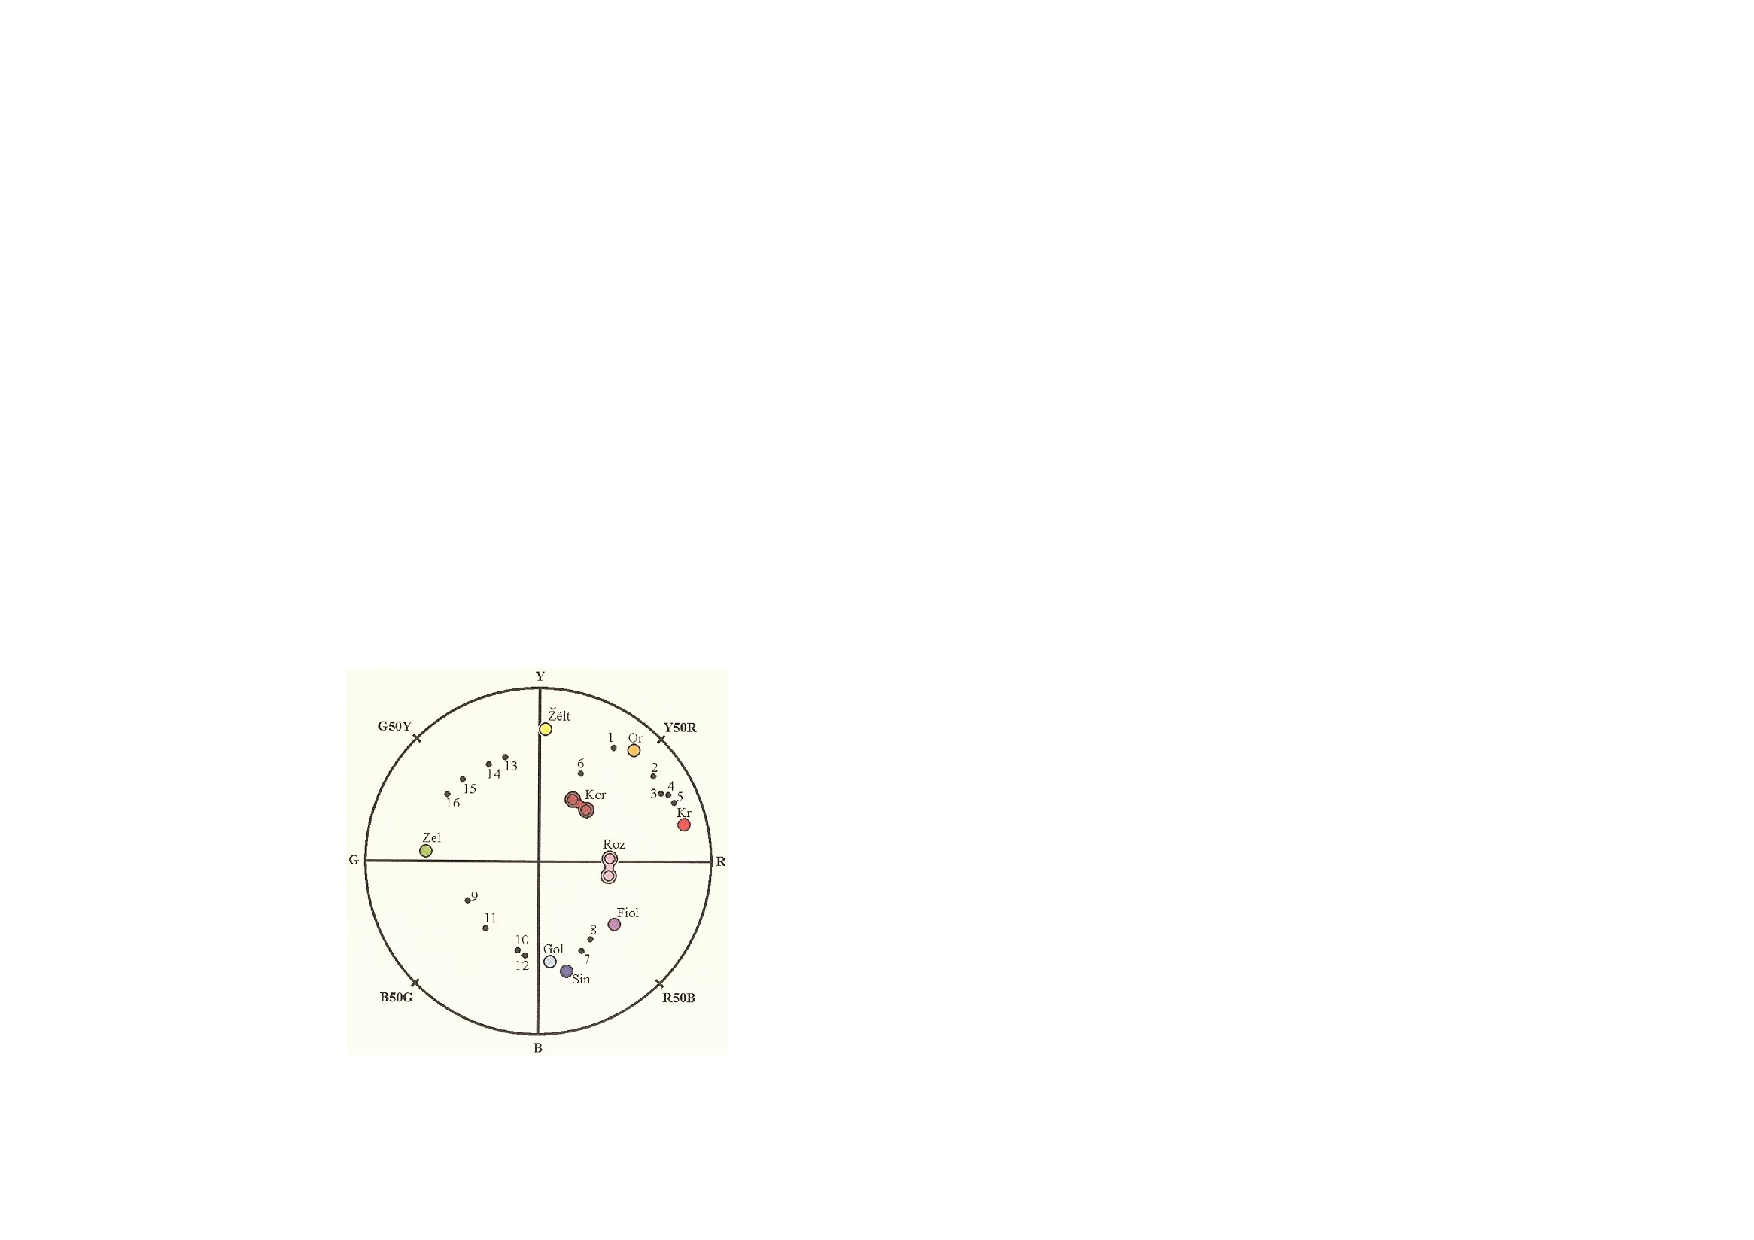
\includegraphics[width=0.6\textwidth]{./category-combination/figures/russian-combination.pdf}
    \caption[Compound chromatic terms in Russian]{Compound chromatic
      terms projected on the hue plane of the NCS colour space. The
      second term in the compound clearly has a bigger impact on the
      resulting focal colour than the first one. The colours between
      \textit{\v z\"eltyj} (`yellow') and \textit{zel\"enyj} (`green') are for
      example named: (13) \textit{zelenovato-\v z\"eltyj}
      (`greenish-yellow'), (14) \textit{zel\"eno-\v z\"eltyj} (`green-yellow'),
      (15) \textit{\v z\"elto-zel\"enyj} (`yellow-green') and (16) \textit{\v z\"eltovato-zel\"enyj} (`yellowish-green'). Figure from
      \cite{safuanova07russian}.}
    \label{f:ccs-russian}
  \end{center}
\end{figure}

To summarise, I have to account for three basic observations: category
combination can be asymmetrical in the sense that one colour category
is deemed more important than the other. This combination can be
modulated through markers in language and the same colour category can
be repeated in the same utterance to give emphasis to indicate it is a
good example of a particular colour category.

\section{Related research}
\label{s:ccs-related-research}

Several suggestions have been made on how the combination of concepts
should be modelled. In certain situations, some compatible properties
can be changed in the base concept, such as in \textit{green apple}. In
other situations, the mapped properties are not compatible and
overrule the corresponding properties in the base concept, such as in
\textit{pink elephant}.

But the combination of concepts is actually not as clear cut, as the
actual modification depends on the context in which it is
used. Consider the Russian example below which states there are many
\textit{red cows} in the Ural mountain range. These cows are of course not
of a bright red colour, but are rather more ginger-coloured
\citep{tribushinina08cognitive}.

\ea
\gll Na Urale mnogo krasnyh korov.\\
On Ural-\textsc{loc} many red-\textsc{pl.gen} cows-\textsc{gen}\\
\glt `There are a lot of red cows in the Urals.'\\
\z


The actual colour implied by the colour adjectives is dependent on
the context in which it is used. The actual colour implied by the
adjective \textit{red} is different whether it is used in the context of
wine, hair, skin, or indeed cows. This is why the use of contrast
classes is suggested. These define a subregion of colours that some
base class is usually associated with, for example the set of all skin
colours. The set of colour categories is transformed into this
subregion. For example, \textit{white skin} does refer to a colour that
would normally be named pinkish and \textit{black} refers to the darkest
colour of skin \citep{gardenfors04conceptual}.

\subsection{Models}

The colour naming model proposed by
\citeauthor{lammens94computational} sorts all categories based on the
similarity to the colour sample that needs to be named and deployed
some heuristics to include the secondmost similar category using
diminuatives such as \textit{-ish} and \textit{somewhat x-ish}
\citep{lammens94computational}. Other colour naming models, store
different centroids for each compound colour term, including the
combination of basic colour terms \citep{mojsilovic05computational}.

\section{Semantic template}
\label{s:ccs-semantic-template}
\is{semantic template!for category combination strategy}

As I am pursuing a compositional approach to semantics, I start from
the semantic network of the basic colour strategy and extend it by
adding a second categorisation process. As the first categorisation
process is strict, it would be unproductive to use the same category
set as it would just return the exact same colour category. In order
for the second categorisation process to be useful, the category set
needs to be modified.

The most naive way to modify the category set is to remove the
category that was used during the first categorisation process. This
would allow the second categorisation process to find the category
that is secondmost similar to the colour sample that needs to be
described. This approach would however not be able to account for the
the repetitive use of the same colour term to highlight the similarity
between the colour sample in the colour category, like in Vietnamese.

The transformation I have implemented is to move all the colour
categories in the colour category set towards the category that has
been used during the first categorisation process. This will entail
that the region of the colour space that was first categorised as the
base category will be repartitioned over its adjacent categories. The
centre of that region however, will still be classified as the base
category. An illustration of such a transformation is provided in
Figure \ref{f:ccs-semantics-transformation}.

\begin{figure}[htbp]
\centering
\subfigure[]{
  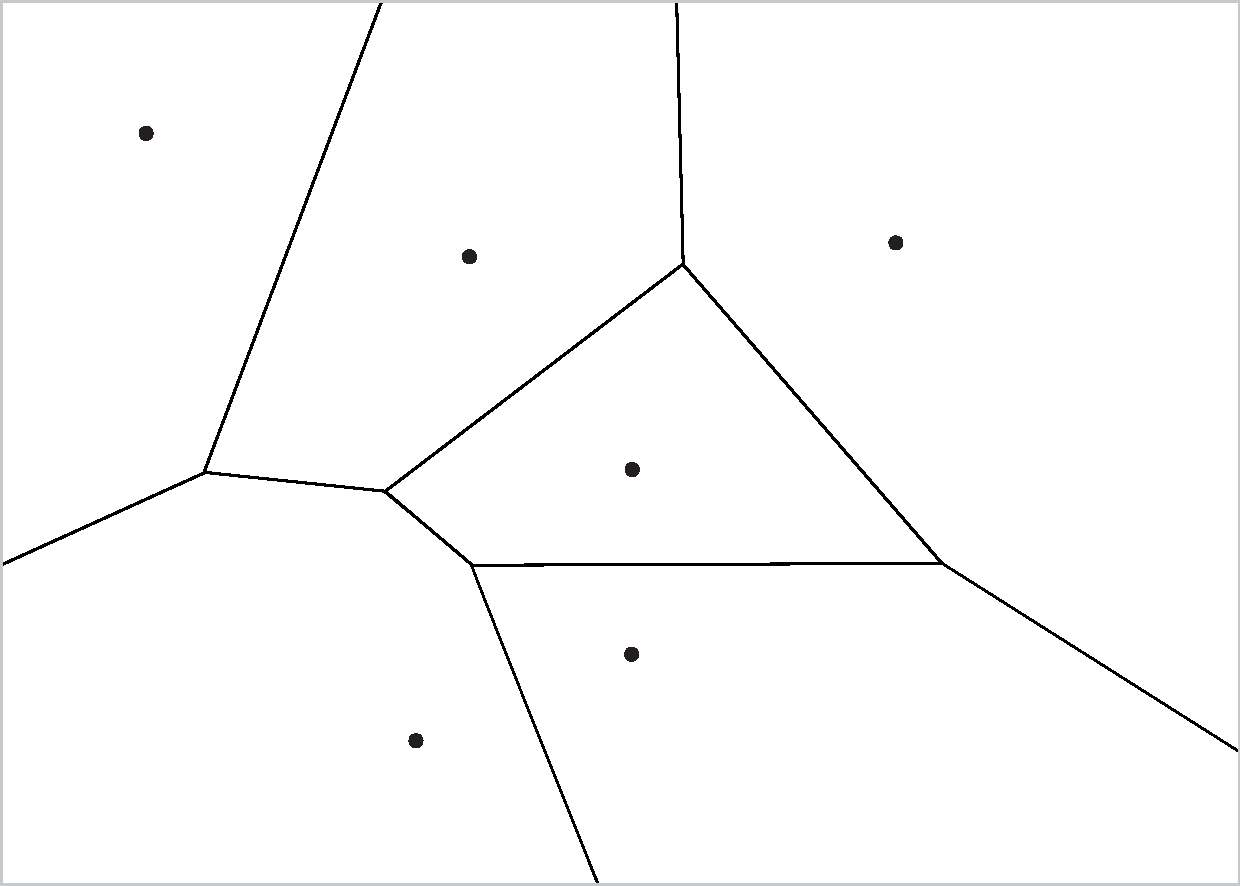
\includegraphics[width=.475\textwidth]{./category-combination/figures/semantics-before-transformation.pdf}
  \label{f:ccs-semantics-before-transformation}
}
\subfigure[]{
  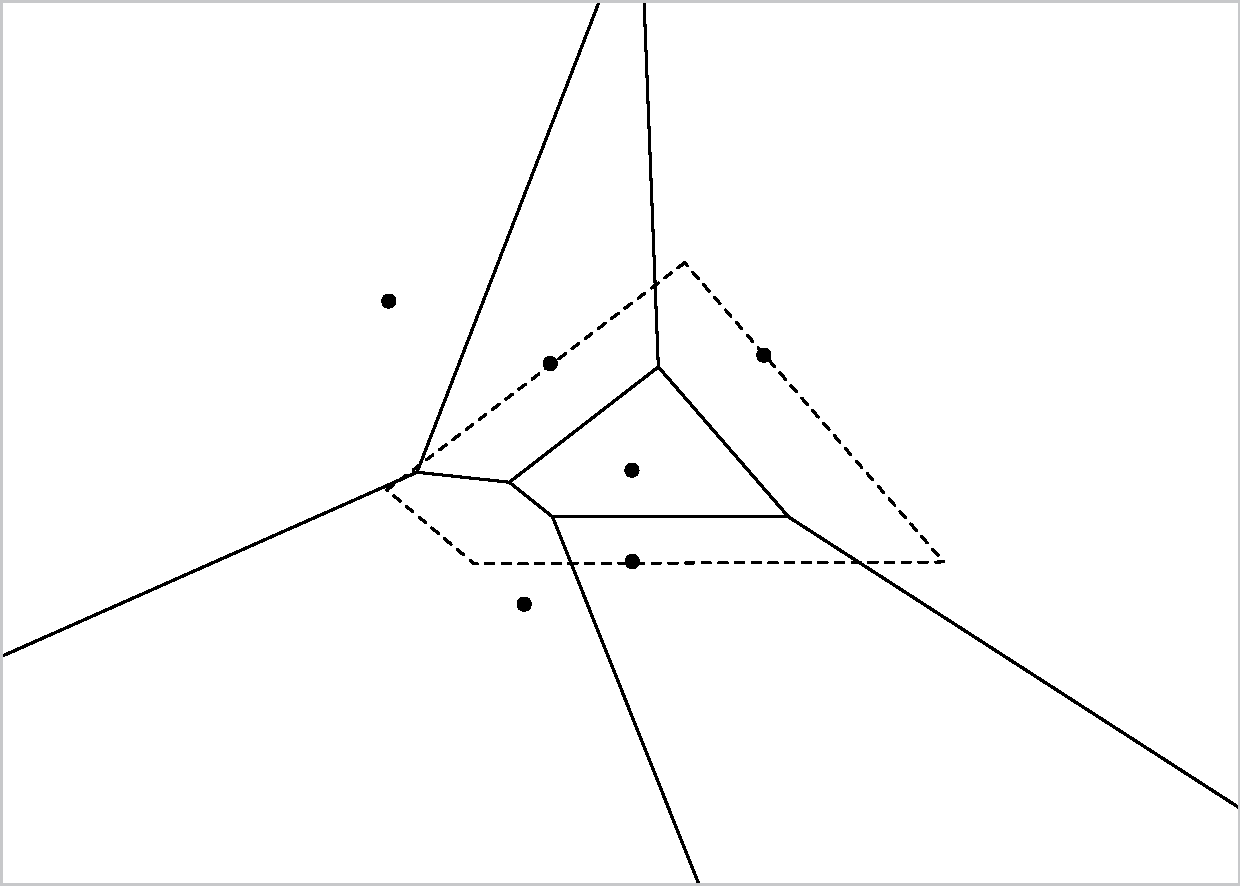
\includegraphics[width=.475\textwidth]{./category-combination/figures/semantics-transformed.pdf}
  \label{f:ccs-semantics-transformed}
}
\caption[Impact of the transformation of the category set in the
category combination strategy on the partitioning of the colour
space]{Impact of the transformation of the category set in the
  category combination strategy on the partitioning of the
  colour space: \subref{f:ccs-semantics-before-transformation}
  partitioning of the colour space before the colour category set is
  transformed; \subref{f:ccs-semantics-transformed} partitioning of
  the colour space after the category set is transformed towards the
  central category. The region that was categorised as
  the base category after the first transformation, is now repartitioned over the categories adjacent
  to the base categories. As the base category is also a member of the
  transformed set, the centre of that region will still be classified
  as the base category.}
\label{f:ccs-semantics-transformation}
\end{figure}

When this second categorisation process would not be constraining
enough to single out a particular colour sample in a context, an
optional categorisation process based on membership can be added.
This process is similar to the one proposed in the graded
  membership strategy but the membership function is now based on the
combined membership of the two categorisation processes instead of
one.

The semantics of the \textsc{category combination strategy} can be
summarised as follows: first all the entities are categorised as in
the basic colour strategy. Next, all categories are drawn
towards the base category that has been used. This transformed
category set is used during the second categorisation
process. Optionally a third categorisation process based on membership
can be added. From the resulting set the entity with the highest
activation is selected.

The proposed semantics satisfy the three requirements outlined at
the beginning of this chapter. Asymmetry is achieved through the
ordering of the categorisation process based on colour: the first one
will define the main region of the conceptual space in which the
sample is to be found; the second one specifies a subregion within
that region. The modulation of the combination process is realised
through the optional categorisation process based on membership. The
repetitive use of a colour category refers to the region that is close
to the repeated colour category.

\subsection{Profiling and first categorisation based on colour}

The profiling and the first categorisation process is identical to the
one of the graded membership strategy. It is a strict
implementation of the categorisation process, as in interpretation
only the samples that are most similar to the interpreted category are
considered for further processing. This decision is based on the
observation that colours that are named using a category combination
will always be most similar to one of its constituent categories, as
supported by the data of Russian compounds \citep{safuanova07russian}.

\subsection{Transformation of the set of colour categories}

The transformation procedure involves moving each colour category
known to the agent in the direction of the base category that was used
during the first categorisation process. Each colour category is moved
to a point on the line segment between the original category and the
base category in the conceptual space of the agent. The new location
is slightly closer to the base category. An illustration of such a
transformation is provided in Figure
\ref{f:ccs-semantics-transformation}.

\subsection{Second categorisation based on colour}

The transformed category set is used for a second categorisation based
on colour. In each entity, the resulting membership value of the first
categorisation process is overwritten by the second categorisation
process, but could also be a function based on these two
functions. Although the first categorisation process is important to
select some samples from the context, I have chosen to overwrite the
value as the actual membership of the second categorisation process
is independent of the membership of the first categorisation
process. For example, a \textit{green-blue} colour sample would have a low
membership during the categorisation with the category for blue, but
could be a very good member of the green category that is transformed
for the category for blue.

This process allows for a further specification of the region in the
conceptual space that was originally categorised as the base category.

\subsection{Optional categorisation based on membership}

An optional categorisation process based on membership can be added to
the chain of processes, which would allow for further specification of
the colour sample. As the membership values stored in the entities now
reflect the second categorisation process, this will specify regions
within the regions that were defined by the previous categorised
process.

\subsection{Selection based on activation}

The selection process is based on the idea that each categorisation
process changes the activation values of each of the entities in the
resulting set. The entity with the highest activation is selected as
the entity resulting from the complete process.

\subsection{Semantic constraint network}

The semantic network for the category combination strategy is
shown in Figure \ref{f:ccs-semantic-program}. The
\textsc{Equal-to-Context} and \textsc{Profile-Colour-Dimensions}
primitives are the same as the ones before. The
\textsc{Filter-by-Colour} primitive is like the one introduced before,
but now has a specific argument of the colour category set it is
applying, as this set might be modified by other primitives. This
requires another primitive \textsc{Get-Basic-Colour-Category-Set} to
retrieve all the categories known to the agent to mimic the old
behaviour of \textsc{Filter-by-Colour}. This category set is also
provided to the \textsc{Draw-Category-Set-to-Category} primitive which
draws all the categories in the direction of the category that is used
during the first categorisation process based on colour. Next another
\textsc{Filter-by-Colour} primitive applies the transformed category
set to the sets filtered by its first instantiation. Finally
\textsc{Select-Most-Activated} returns the most activated entity from
this set as the value for the complete process.  An optional
\textsc{Filter-by-Membership} primitive can be added between the last
two primitives (not shown in figure).

\begin{figure}[htbp]
  \centering
  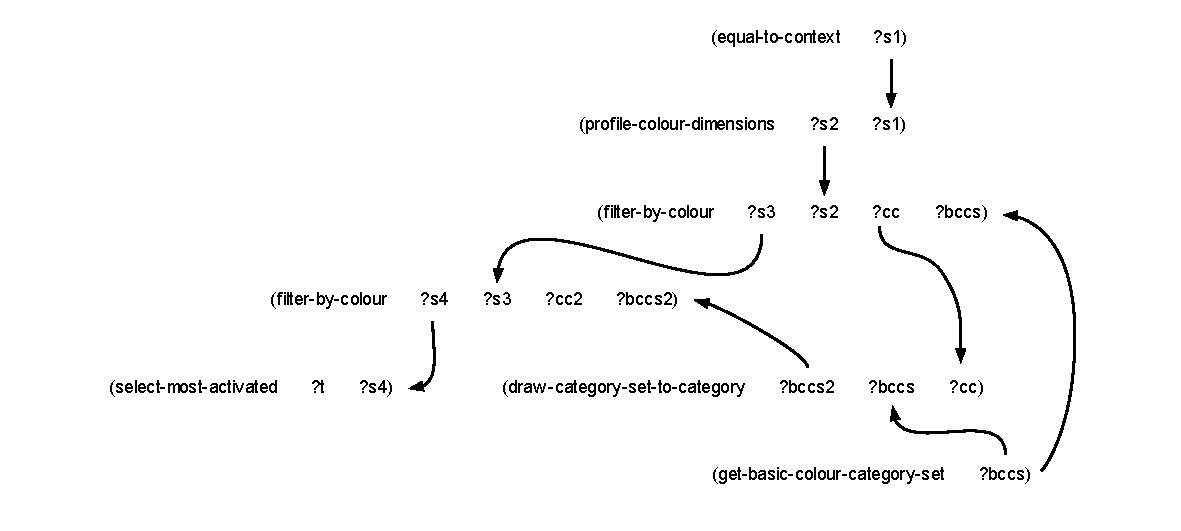
\includegraphics[width=\textwidth]{./category-combination/figures/semantic-program.pdf}
  \caption[The semantic constraint network for the category combination
  strategy]{The semantic constraint network for the category combination
      strategy. Consists of two \textsc{Filter-by-Colour} primitives
    of which the second one deploys a transformed category set. This
    transformation is computed by the
    \textsc{Draw-Category-Set-to-Category} primitive.}
  \label{f:ccs-semantic-program}
\end{figure}

\subsection{Semantic primitives}

\definition{Semantic primitive}{Get-Basic-Colour-Category-Set}

\begin{explanation}{description}
  Retrieves all colour categories known by the agent.
\end{explanation}

\begin{explanation}{slots}
  \verb+?colour-category-set+ (of type category-set)
\end{explanation}

\begin{explanation}{revision specs}
  $\emptyset$: collects all colour categories known to the agent and
  binds it to \verb+?colour-category-set+
\end{explanation}

\definition{Semantic primitive}{Filter-by-Colour}

\begin{explanation}{description}
  Categorises each entity in a source set as the most similar colour
  category in its argument category set. The membership of each entity
  is set to be the similarity to the category it belongs to.
\end{explanation}

\begin{explanation}{slots}
  \verb+?filtered-set+ (of type entity-set) \\
  \verb+?source-set+ (of type entity-set) \\
  \verb+?colour-category+ (of type colour-category) \\
  \verb+?colour-category-set+ (of type category-set)
\end{explanation}

\begin{explanation}{revision specs}
  \verb+?source-set ?colour-category-set+: categorises each entity of
  the source set and returns pairwise bindings for the remaining
  slots; categories to which no entities are assigned, are ignored \\
  \verb+?source-set ?colour-category-set ?category+: computes the
  categorisation of the source set based on all colour categories in
  the category set and when the resulting set for the provided colour
  category is not empty, it gets bound to \verb+?filtered-set+
\end{explanation}

\definition{Semantic primitive}{Draw-Category-Set-to-Category}

\begin{explanation}{description}
  Draws all categories in a category set towards a particular member
  of this category set. When this category is not a member of this
  set, this operation is undefined.
\end{explanation}

\begin{explanation}{slots}
  \verb+?transformed-category-set+ (of type category-set) \\
  \verb+?category-set+ (of type category-set) \\
  \verb+?category+ (of type colour-category)
\end{explanation}

\begin{explanation}{revision specs}
  \verb+?category ?category-set+: draws all categories in the category
  set towards \verb+?category+ bound to \verb+?category+ so that they
  are on the line segment between of \verb+?category+ and the original
  location of the category; the linear factor that determines the
  resulting position is set to 0.4 (where 0 would be equal to
  \verb+?category+ and 1.0 would be the original location of the
  category)
\end{explanation}

\subsection{Alternative approaches to semantics}

Although not implemented nor tested, it has been suggested that fuzzy
sets could support category combinations in a quite natural way. Some
samples belong with full probability to one fuzzy set representing one
basic colour category, but others will be members of more than one
set. If a sample would have a membership of 0.5 to blue and one of 0.5 to
green, it could be named \textit{blue-green}. The \textit{-ish} suffix could be
used for samples with a high membership to one category and up to a
certain membership to another (e.g. samples with memberships 0.7 to
green and 0.3 to blue could be named \textit{bluish green}
\citep{benavente08parametric}).

\section{Syntactic templates}

The syntactic templates that can be used to express this semantic
network are similar to the templates introduced in the previous
chapter. The main difference to the previous templates is that the
rules don't only need to link the variables of the different entity
sets, but also the variables that deal with colour category sets and
colour categories. This is most clear when observing the arguments of
the \textsc{Draw-Category-Set-to-Category} primitive, which requires
the colour category that is used in the first categorisation process
to compute a new colour category set that will be used during the
second categorisation process. The variables related to colour
categories will be dealt with in the \textsc{colour link}, or
\emph{c-link} feature for short.

The linguistic structure for \textit{zel\"eno-\v z\"eltyj} (`green-yellow')
is shown in Figure \ref{f:ccs-linguistic-structure}, in which some
morphological issues are ignored.

\begin{figure}[htbp]
  \centering
  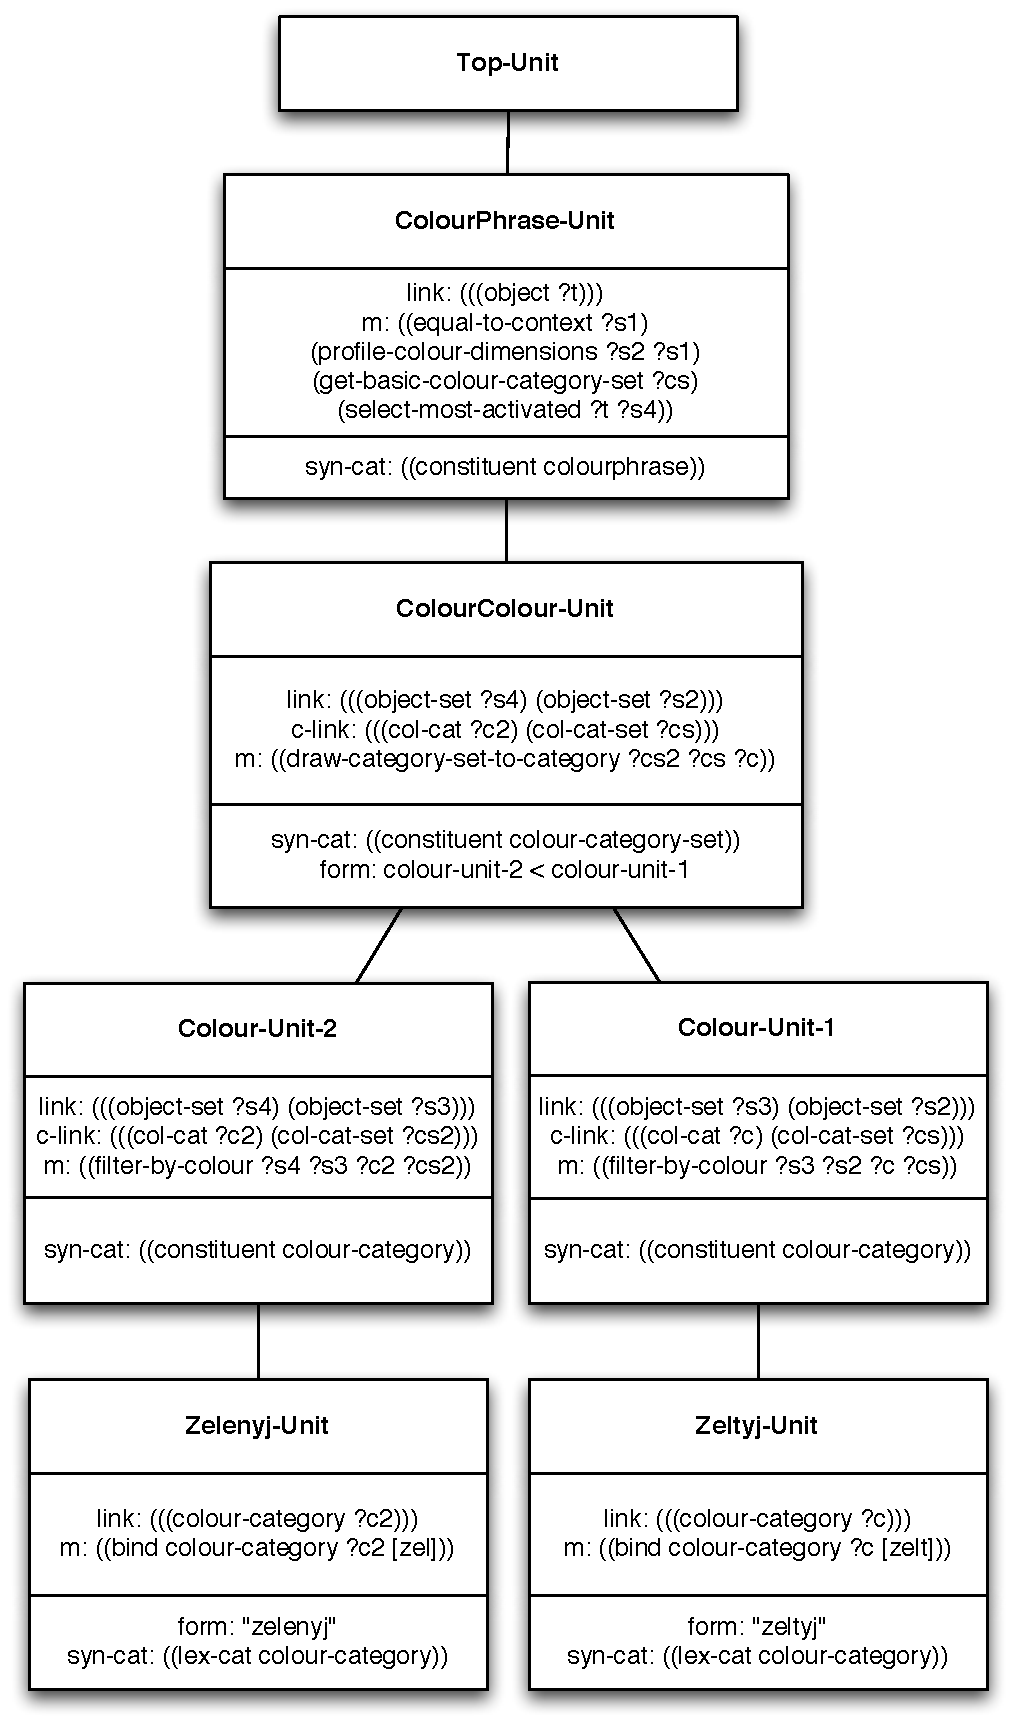
\includegraphics[width=.70\textwidth]{./category-combination/figures/linguistic-structure.pdf}
  \caption[Linguistic structure for category combination
  strategy]{Linguistic structure for category combination
    strategy. Both semantic and syntactic poles are shown in the same
    structure. Semantic information is shown in the top part of each
    unit, the syntactic information in the bottom part of each
    unit. Next to the link features that have been used before to link
    the entity-sets of the primitives together, a c-link feature is
    required to establish variable equalities between primitives for
    the colour categories and the colour category sets.}
  \label{f:ccs-linguistic-structure}
\end{figure}

\subsection{Syntactic template 1.1: Semantic entities}

The semantic entities are dealt with in a similar way as before. I
kindly refer the reader to the previous chapters for examples of
entity rules.

\subsection{Syntactic template 1.2: Functional primitives}
\is{syntactic template!for functional primitives}

The functional rule for \textsc{Filter-by-Colour} is similar to the
one introduced before, but now also provides a \emph{c-link} feature
in which the variables of its colour category and the colour category
set are stored. The category needs to be available to the rest of the
semantic network for when it should be needed for a transformation of
the colour category set. The colour category set is required to allow
for transformed colour category sets to be used by the filtering
process.

\footnotesize
\ltitle{Functional rule for Filter-by-Colour}
\begin{lstlisting}
((?top-unit
  (sem-subunits (?colour-category-unit)) 
  (tag ?meaning
       (meaning ((filter-by-colour ?s3 ?s2 ?c ?cs)))))
 (?colour-category-unit 
  (link (((colour-category ?c)))))
 ((J ?filter-by-colour-unit ?top-unit (?colour-category-unit))
  ?meaning
  (link (((entity-set ?s3) (entity-set ?s2))))
  (c-link (((colour-category ?c) (colour-category-set ?cs))))))
<-->
((?top-unit 
  (syn-subunits (?colour-category-unit)))
 (?colour-category-unit 
  (syn-cat ((lex-cat colour-category))))
 ((J ?filter-by-colour-unit ?top-unit (?colour-category-unit))
  (syn-cat ((constituent colour-category)))))
\end{lstlisting}
\normalsize

\subsection{Syntactic template 1.3: Contextual primitives}
\is{syntactic template!for contextual primitives}

The basic colour strategy is now redefined 
using the \textsc{Filter-by-Colour} primitive as defined in this
chapter. The contextual rule that is needed for this strategy
is very similar to the contextual rule in Section
\ref{s:bcs-contextual-primitive}, except that it now also encapsulates
a \textsc{Get-Basic-Colour-Category-Set} primitive of which the argument is part of
the c-link of the subunit.

\footnotesize
\ltitle{ColourPhrase rule for Basic Colour Strategy}
\begin{lstlisting}
((?top-unit
  (sem-subunits (?colour-unit))
  (tag ?meaning
       (meaning ((select-most-activated ?t ?s3)
                 (profile-colour-dimensions ?s2 ?s1)
                 (equal-to-context ?s1)
                 (get-basic-colour-category-set ?cs)))))
 (?colour-unit
  (link (((entity-set ?s3) (entity-set ?s2))))
  (c-link (((colour-category ?c) (colour-category-set ?cs)))))
 ((J ?colourphrase-unit ?top-unit (?colour-unit))
  ?meaning
  (link (((colour-entity ?t))))))
<-->
((?top-unit 
  (syn-subunits (?colour-unit)))
 (?colour-unit 
  (syn-cat ((constituent colour-category))))
 ((J ?colourphrase-unit ?top-unit (?colour-unit))
  (syn-cat ((constituent colourphrase)))))
\end{lstlisting}
\normalsize

\subsection{Syntactic template 2.2: Re-use of constructions}
\is{syntactic template!re-use of constructions}

An extended version of syntactic template 2.1 needs to be
introduced. The resulting rule looks similar to the one introduced
before, but additionally the rule needs to take care of two
additional aspects. First it needs to be able to cover some
meaning. For the current semantic template, this would be the
\textsc{Draw-Category-Set-to-Category} primitive. And second, it needs
to provide the correct colour link of the new unit.

\footnotesize
\ltitle{ColourColour rule}
\begin{lstlisting}
((?top-unit
  (sem-subunits (?unit-2 ?unit))
  (tag ?meaning
       (meaning ((draw-category-set-to-category ?cs2 ?cs ?cc)))))
 (?unit-2
  (link (((entity-set ?s3) (entity-set ?s2))))
  (c-link (((colour-category ?cc2) (colour-category-set ?cs2)))))
 (?unit
  (link (((entity-set ?s2) (entity-set ?s1))))
  (c-link (((colour-category ?cc) (colour-category-set ?cs)))))
 ((J ?colourcolour-unit ?top-unit (?unit-2 ?unit))
  ?meaning
  (link (((entity-set ?s3) (entity-set ?s1))))
  (c-link (((colour-category ?cc2) (colour-category-set ?cs))))))
<-->
((?top-unit
  (syn-subunits (?unit-2 ?unit))
  (tag ?form 
       (form ((meets ?unit-2 ?unit)))))
 (?unit-2 
  (syn-cat ((constituent colour-category))))
 (?unit 
  (syn-cat ((constituent colour-category))))
 ((J ?colourcolour-unit ?top-unit (?unit-2 ?unit))
  ?form
  (syn-cat ((constituent colour-category)))))
\end{lstlisting}
\normalsize

\section{Baseline experiment}
\is{baseline experiment!for category combination strategy}

In the baseline experiment, I will compare three different language
systems. All language systems are based on the Russian basic colour
categories \citep{safuanova07russian}. The first one is based on the
strict version of the basic colour strategy, the second one is
based on the variant of the category combination strategy
without the additional categorisation based on membership and the
third language system is based on the graded variant of this strategy.

The exact location of the chromatic colour terms in Russian have been
determined \citep{safuanova07russian}. These categories were reported
in the Natural Color System and have been converted to the CIE
$L^*a^*b^*$ colour space using the method described in Appendix
\ref{s:NCS}. Only the location of the chromatic colour categories has
been determined which include two hues for the region English speakers
would call \textit{blue}: \textit{sinij} (`dark blue') and \textit{goluboj} (`light
blue'). The basic colour categories are shown in Figure
\ref{f:ccs-russian-basic}.

\begin{figure}[htpb]
  \centering
  
\includegraphics[height=1.25cm]{./category-combination/figures/russian-basic-categories.pdf}
  \caption[The basic chromatic colour categories for Russian]{The
    basic chromatic colour categories for Russian based on the work of
    \citeauthor{safuanova07russian}. From left to right: \textit{krasnij}
    `red', \textit{oran\v zevyj} `orange', \textit{\v z\"eltij} `yellow', \textit{zel\"enyj}
    `green', \textit{sinij} `dark blue', \textit{goluboj} `light blue',
    \textit{rozovyj} `rose', \textit{fioletovyj} `purple' and \textit{kori\v cnevyj}
    `brown'.}
  \label{f:ccs-russian-basic}
\end{figure}

The same study reports on the exact location of some chromatic
compounds. As a first qualitative test, I will verify whether the
proposed semantics and syntax will name the reported locations in a
similar way. An example from the study lists the chromatic compounds
between \textit{\v z\"eltyj} (`yellow') and \textit{zel\"enyj} (`green') which are
reproduced in Figure \ref{f:ccs-russian-compounds}.

\begin{figure}[htpb]
  \centering
  
\includegraphics[height=1.25cm]{./category-combination/figures/russian-compounds.pdf}
  \caption[Example of colour compounds in Russian]{Example of colour
    compounds in Russian \citep{safuanova07russian}. From left to
    right: (a) \textit{\v z\"eltyj} `yellow', (b) \textit{zelenovato-\v z\"eltyj} 
    `greenish-yellow', (c) \textit{zel\"eno-\v z\"eltyj} `green-yellow',
    (d) \textit{\v z\"elto-zel\"enyj} `yellow-green', (e) \textit{\v z\"eltovato-zel\"enyj}
    `yellowish-green', (f) \textit{zel\"enyj} `green'.}
  \label{f:ccs-russian-compounds}
\end{figure}

For this naming benchmark, \is{naming benchmark!for category combination strategy}
I use an agent that is knowledgeable about
the basic colour strategy and the category combination
  strategy (both the graded and the ungraded variant) and an implementation of the
basic colour categories of Russian (as shown in Figure
\ref{f:ccs-russian-basic}). Next, I run the production procedure and
check what utterances are produced for the chips shown in Figure
\ref{f:ccs-russian-compounds}. When more than one strategy is capable
of reaching the communicative goal, the strategy in which the topic
entity has the highest activation is selected. This activation
reflects the membership of the last categorisation process.

The results of this naming benchmark are shown in Table
\ref{t:ccs-russian-naming-benchmark}. Five out of six colour samples
are named correctly. The one chip that (d) cannot be named is the
yellow-green one. This is due to the first categorisation process
based on colour, which categorises the (a-d) as \textit{\v z\"eltyj}. Only (a-c)
are discriminable by one of the provided language strategies. This
example does not include the morphological complexities of the Russian
language.

\begin{table}[htpb]
  \centering
  \begin{tabular}{l>{\itshape}l>{\itshape}l}
  \lsptoprule
    & \normalfont expected name & \normalfont produced name \\
    \midrule
    (a) & \v z\"eltyj & zeltyj \\
    (b) & zelenovato-\v z\"eltyj  & zelenyj -ato zeltyj \\
    (c) & zel\"eno-\v z\"eltyj & zelenyj zeltyj \\
    (d) & zelto-zelenyj & \normalfont -- \\
    (e) & \v z\"eltovato-zel\"enyj & zeltyj -ato zelenyj \\
    (f) & zel\"enyj & zelenyj \\
    \lspbottomrule
  \end{tabular}
  \caption[Naming benchmark for Russian colour compounds]{Naming benchmark for Russian colour compounds. Five out of six samples are named correctly. The one sample that can not be named is wrongly categorised as \textit{zeltyj} during the first categorisation process based on colour.}
  \label{t:ccs-russian-naming-benchmark}
\end{table}

\begin{figure}[p]
  \centering
  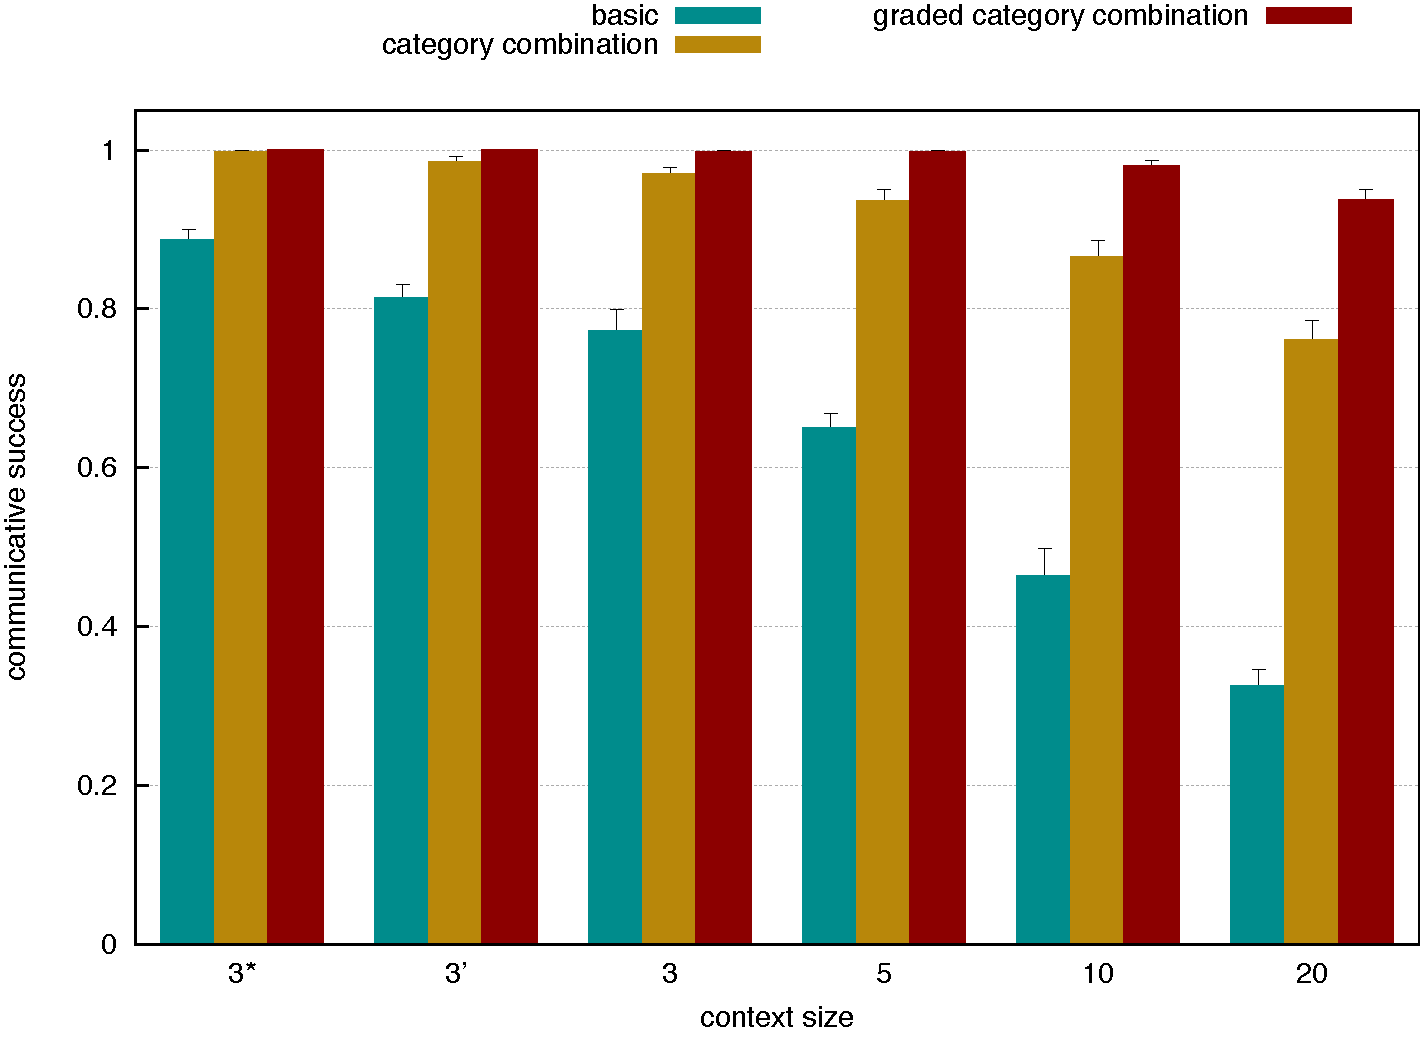
\includegraphics[width=.8\textwidth]{./category-combination/figures/baseline.pdf}
  \caption[The baseline communicative success for category combination
  strategy]{The baseline communicative success for category
    combination strategy, comparing three different language systems
    based on Russian (9 terms). The first system is based on the basic
    colour strategy, the second on the category combination strategy
    and the third one on the graded category combination
    strategy. Allowing agents to combine basic categories results in
    higher communicative success. This effect is increased by adding
    another categorisation process based on membership.}
  \label{f:ccs-baseline}
\end{figure}

\subsection{Results}

The resulting baseline communicative success is shown in Figure
\ref{f:ccs-baseline}. The communicative success for the system in
which agents are allowed to combine categories is higher than when
they are restricted to their basic usage. The communicative success
for the system in which an additional categorisation process based on
the membership is added, is even higher. The richer the semantics the
agents are allowed to use, the higher the resulting communicative
success.

As the number of colour samples in one context increases, the
performance of each of the strategies decreases. The basic
  colour strategy is most prone to this phenomenon. Being able to
combine colour categories compensates for most of the loss. An
additional categorisation process based on membership, results in a
language system that is quite successful, even in very large contexts.

Compared to the English basic colour system (shown in Figure
\ref{f:gms-baseline}), the baseline communicative success for Russian
is lower. This is due to the lower number of basic colour categories
that are reported for the Russian system (9 compared to 11 for
English). The study on Russian colour categories only reports on
chromatic colour categories, and therefore does not specify locations
of the achromatic colour categories (white, grey and black).


\section{Conclusion}

In this chapter, I have introduced a compositional semantics for the
category combination strategy and linguistic rules to express
this semantics in language. Using a naming benchmark, I have
qualitatively compared the resulting names to these reported for the
Russian language. I have shown the positive impact of combining
colour categories on the baseline communicative success. This impact
was even higher when the category combination process was extended
to include a categorisation process based on membership.

\newpage
\thispagestyle{empty}

\chapter{Basic modification strategy}
\label{s:basic-modification-strategy}
\label{s:last-strategy}
\is{language strategy!for colour!basic modification strategy}
\is{basic modification strategy|see{language strategy}}

Next to the basic colour strategy, most languages allow to
specify certain aspects of a colour through the use of modifiers. In
English and Chinese, the use of ``basic'' modifiers accounts for a high
number of colour descriptions in unconstrained naming experiments
\citep{simpson91sex, lin01unconstrained}. The basic modifiers are
defined as the ones that are the most frequently used, which in
English correspond to \textit{bright}, \textit{dull}, \textit{light}, \textit{pale},
etc. In general they specify the lightness or the chromaticity aspect
of a certain colour.

Although basic modifiers are quite commonly used, only a few
papers report on the exact transformation that is implied by these
modifiers. One exception to this rule is a study on the Russian
language, for which the location of the modified categories has been
determined. An example of such an analysis is shown in Figure
\ref{f:ams-russian-diagram}. The modifiers \textit{t\"emno-} (`dark') and
\textit{svleto} (`light'), modify the focus of the basic category parallel to the blackness dimension (W-S). The modifiers \textit{bledno-} (`pale') and \textit{jarko-} (`bright') shift the chromaticity of the basic colour
category. This shift is parallel to the W-C dimension for lighter
colours and parallel to the S-C dimension for darker colours
\citep{safuanova07russian}.

\begin{figure}[htpb]
  \centering
  \includegraphics[width=.5\textwidth]{./achromatic/figures/russian-diagram.pdf}
  \caption[Location of modified basic colour foci in Russian]{Location
    of modified basic colour foci in Russian projected into the NCS
    blackness-chromaticity triangle. \textit{t\"emno-} `dark' (solid
    circle), \textit{jarko-} `bright' (sun), \textit{svetlo-} `light'
    (open circle) and \textit{bledno-} `pale' (dashed circle). Figure
    from \cite{paramei05singing}.}
  \label{f:ams-russian-diagram}
\end{figure}

\section{Related research}

The suggestions made in the literature about how to implement the
combination of a basic modifier and a basic colour category are
similar to those reported for the category combination strategy
(see Section \ref{s:ccs-related-research}) as the basic
  modification strategy could be thought of as a special case of that
strategy.

The process of mapping a set of properties to a specific category can
not be seen as a straightforward overwriting of a specific property
in the base category. For example, a light brown sample is still
darker than a dark yellow sample. So instead of overwriting the
lightness value of the base category with an absolute value, the
modifiers alter the values specified by the base category. As a
result, basic modifiers are relative to the base category they
modify.

Alternatively, the semantics of a combination of a basic
modifier and a basic colour category could be thought of as a context
dependent filtering operation. First, all entities that are categorised
as the basic colour category would be selected from the context. Next,
the average lightness value of the remaining entities could be used to
decide which entity should be named \textit{dark} and which should be named
\textit{light}. Although this could be a productive strategy, using  average lightness
values of the remaining entities might yield unwanted results. For example, 
if the contexts would consist for example of
only two very light green colour samples, it would be unlikely one would
be called \textit{light green} and the other one \textit{dark green}. Moreover,
human subjects are able to assign prototypical colour samples to each
description independent of the context in which the colour samples are
presented \citep{safuanova07russian}.

\section{Semantic template}
\is{semantic template!for basic modification strategy}

I hypothesise that the agents maintain different sets of categories,
which each specify a mutual exclusivity relation between its
members. One such set is the set of basic colour categories. For
example, a colour can not at the same time be red and green. A similar
relation holds for the lightness modifiers \textit{light-} and \textit{dark-}:
a colour is considered to be either light or dark and can never be
light and dark at the same time. This relation is represented by
organising colour categories in different sets. Another set of
categories could be those that specify the chromaticity of a
particular colour, like \textit{pale-} and \textit{bright-}.

The approach of agents maintaining several category sets, ensures a
uniform treatment of each of these sets in all of the strategies
introduced before. This allows for example to only specify some
dimensions of a colour sample, as in \textit{bright green}, or to specify
graded membership, as in \textit{darkish red}.

As I am still pursuing a compositional semantics, I will start from
the semantics of the category combination strategy, as this is
already quite similar to the semantics needed for the current
strategy. The transformation proposed for that strategy can not be
applied anymore, as the modifier category is not a member of the basic
colour category set.

The transformation I propose, shifts the modifiers to the borders
defined by the other basic colour categories. So for example, let us
suppose the base category is yellow. The light modifier will now be
shifted to the border with the white category and the dark modifier to
the border with the brown category. A schematic representation of this
operation is shown in Figure \ref{f:ams-semantics-schematic}.

\begin{figure}
\centering
\subfigure[]{
  
\includegraphics[width=.3\textwidth]{./achromatic/figures/semantics-achromatic.pdf}
  \label{f:ams-semantics-basic}
}
\subfigure[]{
  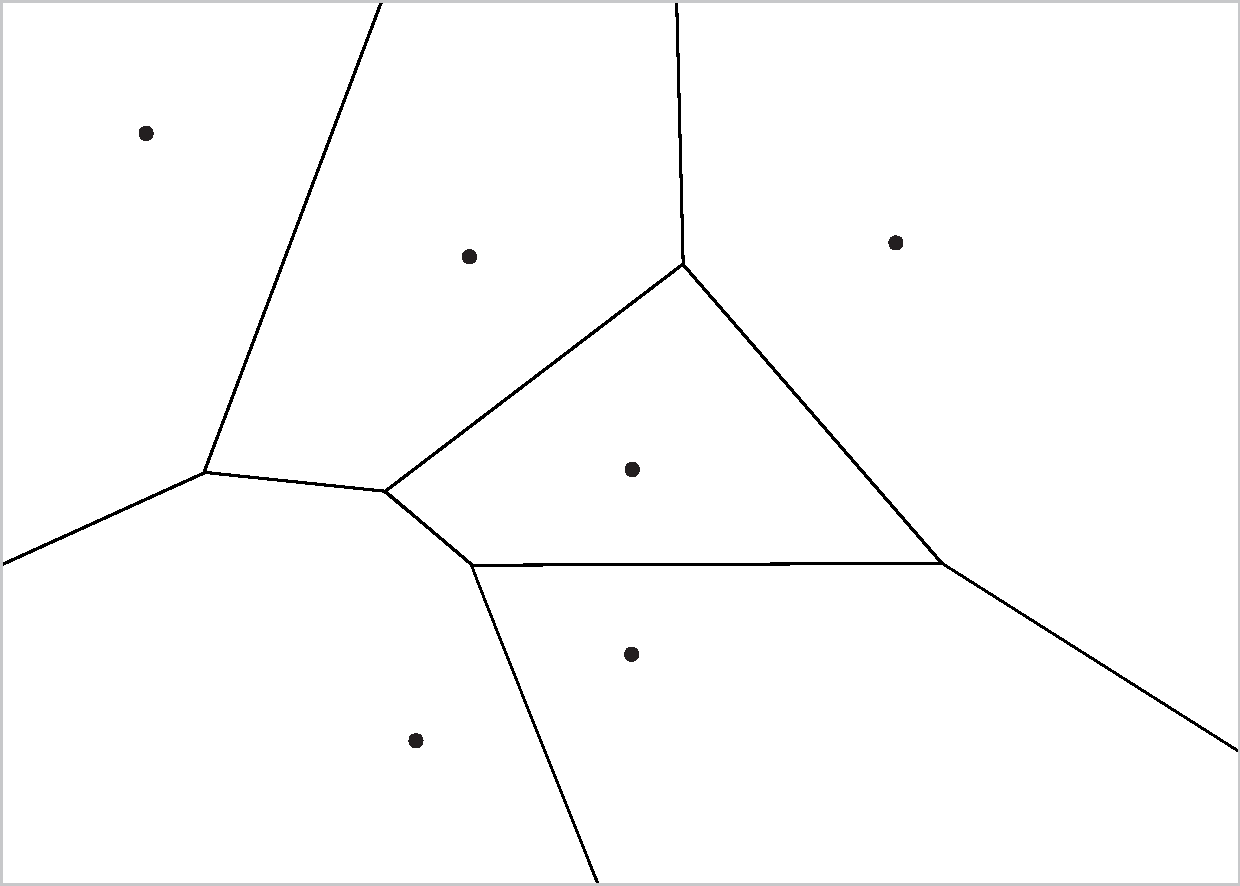
\includegraphics[width=.3\textwidth]{./achromatic/figures/semantics-basic-categories.pdf}
  \label{f:ams-semantics-basic-categories}
}
\subfigure[]{
  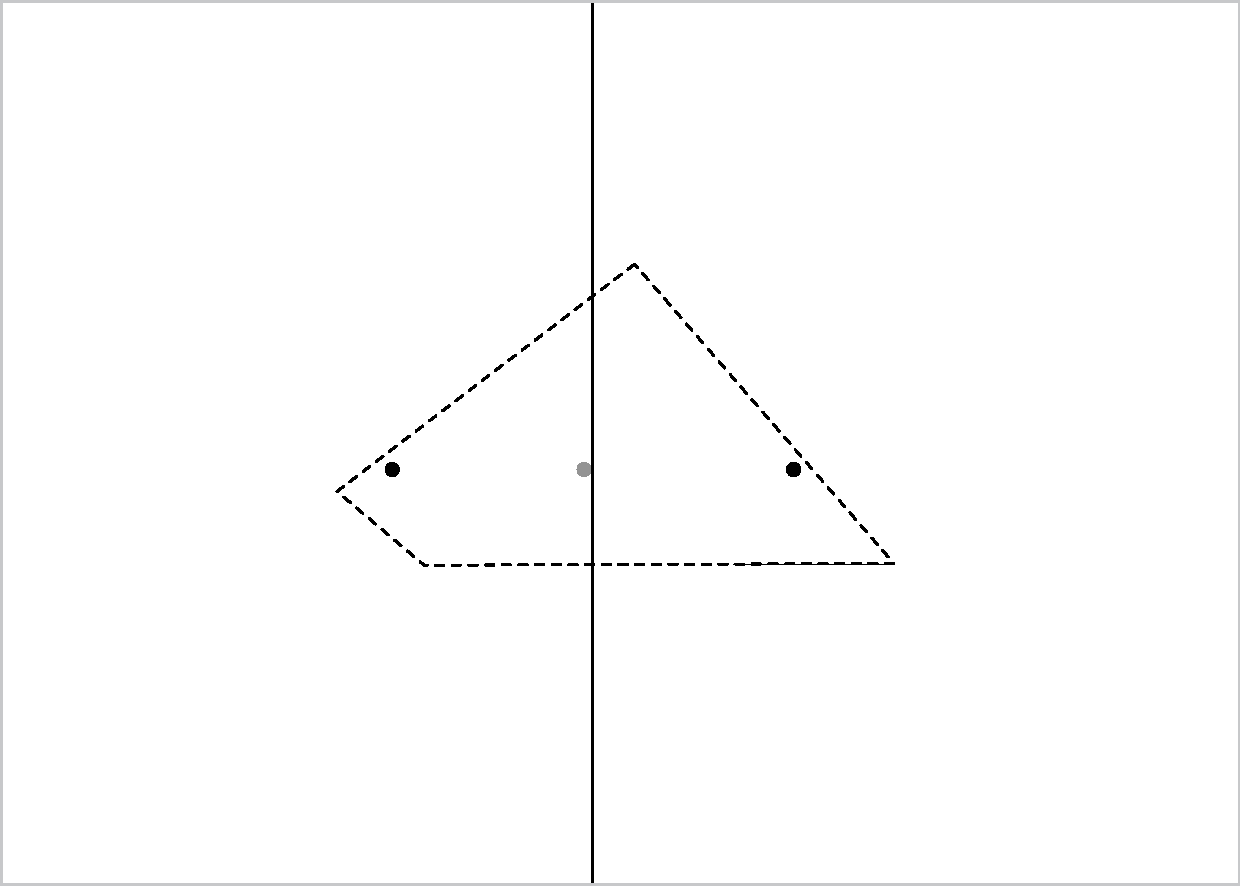
\includegraphics[width=.3\textwidth]{./achromatic/figures/semantics-achromatic-transformed.pdf}
  \label{f:ams-semantics-basic-transformed}
}
\caption[Schematic representation of the transformation for basic
modifiers]{Schematic representation of the transformation for
  basic modifiers: \subref{f:ams-semantics-basic} the
  partitioning of the colour space based on two basic modifiers;
  \subref{f:ams-semantics-basic-categories} the partitioning of the
  colour space based on the basic colour categories;
  \subref{f:ams-semantics-basic-transformed} the transformation
  of the basic modifiers towards one of the basic colour
  categories. The transformed basic modifiers lie on the border
 of the basic colour category.}
\label{f:ams-semantics-schematic}
\end{figure}

The semantics of the basic modification strategy can be
summarised as follows: first a normal categorisation similar to the
one in the basic colour strategy is performed. Before the
basic modifiers are applied, they are transformed corresponding
to the base category that is used during the first categorisation
process. Next the most activated entity is selected from the resulting
set. This process can potentially be extended by a categorisation
process based on activation.

\subsection{Profiling and first categorisation based on colour}

The profiling and the first categorisation process is identical to the
one of the graded membership strategy. It is a strict
implementation of the categorisation process, as in interpretation
only samples that are most similar to the interpreted category are
considered for further processing. This decision is based on the
observation that for basic modifiers, the base category is always
the one that is most similar to the colour sample
\citep{safuanova07russian}.

\subsection{Transformation of set of modifying categories}

Based on the category used during the first categorisation process,
the basic modifiers are transformed in such a way they represent 
the partitioning defined by the basic colour categories. This
operation is based on an iterated estimation procedure in which the
location of the modifier is estimated on the line section between the
modifier and the base category. Each time the new location is
estimated, it is reified as a colour sample that is classified using
the basic colour category set. This procedure stops when the new
location is close to the borders of the base category.

The modifying categories are represented as any other colour category,
but also specify a weight for each dimension representing how
relevant this dimension is. For the lightness modifiers, this would
mean that only the lightness dimension is relevant ($L^*$ in the CIE $L^*a^*b^*$ colour
space). For the chromaticity modifiers, this would be the two hue
dimensions ($a^*$ and $b^*$ in the same colour space). When there are two
categories the resulting coordinates are determined based on these
weights: the lower the weight, the less a particular category
contributes to that dimension.

\subsection{Second categorisation based on modifiers}

Once the modifier categories are transformed, they are used for a
second categorisation process. Like in the category combination
  strategy the membership value of the first categorisation process
is overwritten by the one resulting from the second categorisation
process for similar reasons. A \textit{light-brown} colour sample could
have a low membership for the base category brown, but might be a very
good member of the light modifier after it is transformed for
brown. This second categorisation process allows the agent to further
specify the subregion of the conceptual space that was classified as
the base category.

\subsection{Optional categorisation based on membership}

An optional categorisation process based on membership can be added to
the process, which allows for a further specification of the subregion
of the colour space. This additional process allows to describe
samples as \textit{darkish green} or \textit{very light yellow} and could be
added when the subsequent categorisation process is not sufficient to
discriminate a particular colour sample in a context.

\subsection{Selection based on activation}

The selection is based on the membership value that can be altered by
each of the categorisation processes. The entity with the highest
activation is selected as the entity resulting from the complete
process.

\subsection{Semantic constraint network}

The complete semantic network for the basic modification
  strategy is shown in Figure \ref{f:ams-semantic-structure}. It is
very similar to the one for the category combination
  strategy. The first categorisation process based on the basic
colour category set is entirely identical. The
\textsc{Get-Lightness-Category-Set} retrieves the lightness
modifiers known to the agent. The
\textsc{Scale-Category-Set-to-Category} transforms this category set
to the category that was used during the first categorisation
process. The resulting category set is used by the second
\textsc{Filter-by-Colour} operation. Finally,
\textsc{Select-Most-Activated} returns the entity with the highest
entity from the resulting set. An optional
\textsc{Filter-by-Membership} primitive can be added between the last
two primitives.

\begin{figure}[htpb]
  \centering
  \includegraphics[width=\textwidth]{./achromatic/figures/semantic-program.pdf}
  \caption[Semantic constraint network for basic
  modifiers]{Semantic constraint network for basic modifiers. The
    network consists of two \textsc{Filter-by-Colour} primitives. The
    first uses the basic colour category set, the second the
    lightness modifiers which are transformed into the category used
    by the first categorisation process. This transformation is
    computed by the \textsc{Scale-Category-Set-to-Category}
    primitive.}
  \label{f:ams-semantic-structure}
\end{figure}

\subsection{Semantic primitives}

\definition{Semantic primitive}{Get-Lightness-Colour-Category-Set}

\begin{explanation}{description}
  Retrieves all lightness known by the agent.
\end{explanation}

\begin{explanation}{slots}
  \verb+?colour-category-set+ (of type category-set)
\end{explanation}

\begin{explanation}{revision specs}
  $\emptyset$: collects all lightness modifiers known to the agent
  and binds it to \verb+?colour-category-set+
\end{explanation}

\definition{Semantic primitive}{Scale-Category-Set-to-Category}

\begin{explanation}{description}
  Scales all categories in a category set so that they fit into a
  specific category. The borders of that category are determined by
  the other categories in the category set to which that category
  belongs. The category does not need to be a member of the category
  set that is transformed, but the categories of both sets should be
  compatible so they can be successfully combined, like for example
  scaling a set of colour categories to another colour category from
  another category set.
\end{explanation}

\begin{explanation}{slots}
  \verb+?transformed-category-set+ of type \emph{category-set} \\
  \verb+?category-set+ of type \emph{category-set} \\
  \verb+?category+ of type \emph{colour-category}
\end{explanation}

\begin{explanation}{revision specs}
  \verb+?category ?category-set+: scales all categories in the category
  set towards \verb+?category+ bound to \verb+?category+ so that they
  are on the border of \verb+?category+
\end{explanation}

\section{Syntactic templates}

The templates introduced in the previous chapter can be used to cover
each part of the semantic constraint network in Figure
\ref{f:ams-semantic-structure}. The linguistic structure for
``t\"emno-rozovyj'' is shown in Figure
\ref{f:ams-linguistic-structure}.

\begin{figure}[htbp]
  \centering
  \includegraphics[width=.8\textwidth]{./achromatic/figures/linguistic-structure.pdf}
  \caption[Linguistic structure for basic modifiers]{Linguistic
    structure for basic modifiers. The structure is similar to the
    one presented in the previous chapter, but with a different
    instantiated rule based of Syntactic template 2.1 that introduces
    the ModifierColour unit to the structure.}
  \label{f:ams-linguistic-structure}
\end{figure}

\subsection{Syntactic template 2.2: Re-use of constructions}
\is{syntactic template!re-use of constructions}

The syntactic template 2.2 that was introduced in the previous chapter
can also be used to express the parts of the basic
  modification strategy that are not yet covered by any of the other
rules. It encapsulates all remaining primitives t and takes care of
all the needed variable equalities between its subunits and the
contextual rule of the basic colour strategy. It is responsible for
introducing the ModifierColour-unit in Figure
\ref{f:ams-linguistic-structure} in both producing and parsing.

\footnotesize
\begin{Verbatim}[frame=lines, label=ModifierColour rule]
((?top-unit
  (sem-subunits (?modifier-unit ?colour-unit))
  (tag ?meaning
       (meaning ((scale-category-set-to-category ?cs3 ?cs2 ?cc)
                 (get-lightness-category-set ?cs2)
                 (profile-lightness-dimensions ?s3 ?s2)))))
 (?modifier-unit
  (link (((entity-set ?s4) (entity-set ?s3))))
  (c-link (((colour-category ?cc2) (colour-category-set ?cs3)))))
 (?colour-unit
  (link (((entity-set ?s2) (entity-set ?s1))))
  (c-link (((colour-category ?cc) (colour-category-set ?cs)))))
 ((J ?modifiercolour-unit ?top-unit (?modifier-unit ?colour-unit))
  ?meaning
  (link (((entity-set ?s4) (entity-set ?s1))))
  (c-link (((colour-category ?cc2) (colour-category-set ?cs))))))
<-->
((?top-unit
  (syn-subunits (?modifier-unit ?colour-unit))
  (tag ?form 
       (form ((meets ?modifier-unit ?colour-unit)))))
 (?modifier-unit 
  (syn-cat ((constituent colour-category))))
 (?colour-unit 
  (syn-cat ((constituent colour-category))))
 ((J ?modifiercolour-unit ?top-unit (?modifier-unit ?colour-unit))
  ?form
  (syn-cat ((constituent colour-category)))))
\end{Verbatim}
\normalsize

\section{Baseline Experiment}
\is{baseline experiment!for basic modification strategy}

The baseline experiment will compare three different predefined language
systems. Each of them is based on the Russian colour category system
\citep{safuanova07russian}. The first one is based on the strict
version of the basic colour strategy. The second one is based
on the basic modification strategy using 2 basic
modifiers: \textit{svleto} (`light') and \textit{t\"emno} (`dark'). The modifiers
are specified as maximal and minimal lightness values and are only
specified in the lightness dimension. The third language system is
based on the basic modification strategy which includes a
categorisation process based on membership using the same basic
semantic entities.

The foci of the basic and modified colour categories have been
reported in the Natural Color System \citep{safuanova07russian} and
have been converted using the method described in Appendix
\ref{s:NCS}. The resulting foci are shown in Figure
\ref{f:ams-russian-basic-modifiers}.

\begin{figure}[htpb]
  \centering
  \includegraphics[height=3.75cm]{./achromatic/figures/russian-modified-foci.pdf}
  \caption[Foci of modified basic colour categories in Russian]{Foci
    of modified basic colour categories in Russian. The basic colour
    categories are shown in the middle. The top row shows these
    categories modified with \textit{svleto-} `light' and the bottom
    row shows the same categories modified with \textit{t\"emno-}
    `dark'.  From left to right: \textit{krasnij} `red', ``oran\v
    zevyj'' `orange', \textit{\v z\"eltij} `yellow',
    \textit{zel\"enyj} `green', \textit{sinij} `dark blue',
    \textit{goluboj} `light blue', \textit{rozovyj} `rose',
    \textit{fioletovyj} `purple' and \textit{kori\v cnevyj} `brown'.}
  \label{f:ams-russian-basic-modifiers}
\end{figure}

As a first test of the proposed semantics, I run a naming benchmark
over all the colour chips reported in the study (shown in Figure
\ref{f:ams-russian-basic-modifiers})
\is{naming benchmark!for basic modification strategy}. 
I run the production
procedure and compare the resulting names to the ones reported by the
study. The results for this benchmark are quite good: 15 out of 18
modified chips are named correctly. The chips that were named
incorrectly are shown in Table \ref{t:ams-russian-naming-benchmark}

\begin{table}[htpb]
  \centering
  \begin{tabular}{>{\itshape}l>{\itshape}l}
  \lsptoprule
    \normalfont expected name & \normalfont produced name \\
    \midrule
    t\"emno-\v z\"eltij & \normalfont -- \\
    t\"emno-goluboj & svleto-sinij \\
    svleto-sinij & t\"emno-goluboj\\
    \lspbottomrule
  \end{tabular}
  \caption[Naming benchmark for Russian lightness modifiers]{Naming benchmark for Russian lightness modifiers. Only the three samples that were named incorrectly are shown.}
  \label{t:ams-russian-naming-benchmark}
\end{table}

\textit{t\"emno-\v z\"eltij} could not be
named, as it is still considered a light shade of yellow. The names
for the colours samples for \textit{t\"emno-goluboj} (`dark ``light blue''')
and \textit{svleto-sinij} (`light ``dark blue''') were mixed up, as the former
is lighter than the second, which is also reported in literature
\citep{safuanova07russian}. All other colour samples were named
correctly.

\subsection{Results}

The results of the baseline experiment are shown in Figure
\ref{f:ams-baseline}. The language system in which agents can use
basic modifiers reaches a higher level of baseline communicative
success when compared to the basic colour strategy. This
positive impact is even higher when agents are allowed to grade the
resulting membership (compare results of basic modifiers to
graded basic modifiers). The higher the expressivity of the
agents, the higher the resulting baseline communicative success.

When compared to the baseline experiment of the category
  combination strategy, the resulting baseline communicative success
is slightly lower. This is probably due to the lower number of
categories that can be used to modify the basic categorisation
process. In the current experiment, only two such categories are
present, whereas in the category combination experiment, all
adjacent colour categories could be used.

\begin{figure}[htpb]
  \centering
  \includegraphics[width=.8\textwidth]{./achromatic/figures/baseline.pdf}
  \caption[Baseline communicative success for basic modification
  strategy]{Baseline communicative success for basic modification
    strategy. The baseline success of the basic colour strategy is
    lower than the success of the basic modification strategy. When
    this strategy is extended with a categorisation process based on
    membership, the resulting baseline success is even higher.}
  \label{f:ams-baseline}
\end{figure}

\section{Conclusion}

In this chapter I have proposed a semantic template that allows
agents to use basic modifiers. This template is based on
observations in natural language and is highly compositional. This
compositionality allows agents to re-use the semantic primitives and
constructions that have been introduced in previous chapters.

The proposed semantic template in which the lightness categories are
represented in a set of colour categories separate from the
basic colour categories, allows for the re-use of each of the
previous language strategies using these lightness
categories. Representing the semantics of descriptions like \textit{light}
or \textit{very light} requires the simple replacement of the primitive that
retrieves the colour category set from the ontology of an agent.

\part{Self-organisation of language systems}\label{s:evolution-of-language-systems}

\section*{Introduction}

\addtocounter{chapter}{1}
\setcounter{figure}{0}

In the third\todo{was ``second'', changed to ``third''} part of this book, I will study the self-organisation of
language systems that are based on a single strategy. In order to do
so, I need to introduce the adoption, alignment and invention
operators for that strategy. The \textsc{adoption operator}\is{adoption operator|see{learning operators}}\is{learning operators} specifies how language users can pick up items of the language
system. The \textsc{alignment operator}
\is{alignment operator|see{learning operators}}
specifies how agents should
update their linguistic knowledge after a communicative
interaction. The \textsc{invention operator}
\is{invention operator|see{learning operators}}
is triggered when the
(current knowledge of) the language system is insufficient or when the
current language system is considered to be inefficient
\citep{steels06how}.

The performance of the adoption and the alignment operator can be
evaluated in an \textsc{acquisition experiment}\is{acquisition experiment} 
in which one agent
acquires a predefined language system through playing language games.
This evaluation is achieved by comparing the communicative success of the
learner to the communicative success of two agents that share the
predefined language system. The predefined language systems are
implemented as in the baseline experiments in \partref{s:language-strats}.

The invention operator can be evaluated in a \textsc{formation
  experiment}\is{formation experiment} in which a population of
agents needs to construct its own language system based on one
language strategy and allows agents to extend the current language
system. These innovations can be picked up by other agents using the
adoption operators. After each interaction agents align their
knowledge of the language system using the alignment operator. This
alignment operator allows agents to track their (local view on) the
communicative success of certain linguistic items, which they can use
to prefer one linguistic item over the other. At the system level this
mechanism can lead to the dominance of one item over the other and to
the disappearance of items that are disused. The complete process of
how a language strategy can construct a language system is illustrated
in \figref{f:strategies-1}.\enlargethispage{3\baselineskip}

\begin{figure}
  \begin{center}
    \includegraphics[width=0.7\textwidth]{./intro/figures/strategies-1.pdf}
    \caption[The construction of a language system based on a single
    language strategy]{The construction of a language system based on
      a single language strategy. The language strategy allows agents
      to expand the language system. Based on a feedback loop which
      reflects success in communication, an agent can prefer linguistic
      items that are more successful, whereas unsuccessful linguistic items
      can be removed from the language system.}
    \label{f:strategies-1}
  \end{center}
\end{figure}

\addtocounter{chapter}{-1}

\thispagestyle{empty}









\chapter{Basic colour strategy}
\label{s:basic-operators}

\setcounter{figure}{1}

To complete the definition of the basic colour strategy, I need
to introduce its adoption, alignment and invention operator. The
invention operator allows users to expand the current language system
whenever they feel it is insufficient for their communicative
needs. This expansion involves the invention of a new colour category
and a lexical rule to express this category in language. The adoption
operator allows language users to pick up these newly invented terms
and the corresponding colour categories. The alignment operator
specifies how language users can align their linguistic knowledge both
on the syntactic and the semantic level.

\section{Related models}

In Chapter \ref{s:basic-strategy}, I already introduced various models
\citep{steels05coordinating, belpaeme05explaining, belpaeme07language,
  puglisi08cultural, baronchelli10modeling} that adhere to the
language game paradigm and use the colour naming game. The goal of
these studies was to study how a population of agents could coordinate
their own colour category system through local interactions.

Other models for the coordination of a colour category system have
been proposed as well. One model is more in line with the iterated
learning model \citep{smith03iterated} in which the burden of the
explanation is placed on the idea that a language learner will have to
generalise from only a limited number of observations instead of the
communicative function. In this model, colour categories are inferred
using Bayesian inference and invention is based on a random choice
\citep{dowman07explaining}.

Another mathematical model focusses on a discrimination task for which
the expected outcome depends on the similarity of the colours that
need to be discriminated. In this model, a circular conceptual colour
space is deployed, in which any typology of categories is as likely to
occur as others. Adding heterogeneity to the model, either in the
population or in the likelihood that a particular colour is presented
to the agents or both, breaks this symmetry
\citep{komarova08population}.

\section{Adoption and alignment operators}
\label{s:bcs-adoption-alignment-operators}

The main goal of the adoption and alignment operators is to ensure
that one agent can acquire the language system of another agent. It
needs to learn the private knowledge of the language system that is
being used in such a way that is sufficiently coordinated to ensure
communicative success.

The adoption operator\is{learning operators!adoption operator!for basic colour strategy}
is used to learn the colour categories of
another agent that are unknown to the learning agent. The main trigger
for this operator is hearing an unknown colour term. The application
of this operator results in learning a new category that is focussed
on the colour of the topic of the current interaction. The unknown
colour term is associated with this new category. This operator is in
line with research in developmental psychology which showed the
influence of learning a category upon hearing a new label
\citep{xu02role}. Note that this implementation of the adoption
operator implies that no synonyms will be present in the resulting
language system.

The alignment operator\is{learning operators!alignment operator!for
  basic colour strategy} is implemented by shifting the prototype of
the category that was used in the direction of the colour of the
topic. It is used by both speaker and hearer after a successful
interaction. The rate by which this shift happens is controlled by
\textsc{colour category alignment rate} 
\is{alignment rate!colour category} 
\is{colour category alignment rate|see{alignment rate}} 
($r_a$) which linearly specifies the new
location of the prototype ($c_{n+1}$) on the line segment between the
old location of the prototype ($c_n$) and the topic ($t$). The exact
formula is shown in Equation \ref{eq:alignment_rate}. If the alignment
rate is 0, the prototype does not shift at all, whereas at a rate of
1, the new location would be the topic of the last interaction. In all
experiments reported in this book, the alignment rate is fixed to
0.05, unless stated otherwise. An illustration of an alignment rate is
given in Figure \ref{f:alignment-rate}.

\begin{equation}
c_{n+1} = (1 - r_a) c_n  + r_a t
\label{eq:alignment_rate}
\end{equation}

\begin{figure}[htbp]
  \begin{center}
    \includegraphics[width=.55\textwidth]{./basic-operators/figures/alignment-rate.pdf}
    \caption[Illustration of the alignment rate]{Illustration of the
      alignment rate. Before the game, the prototype of the category
      was at (2,3). The colour of the topic sample was located at
      (6,5). Given that the interaction was successful and the
      alignment rate is 0.75, the location of the prototype will
      become (5,4.5).}
    \label{f:alignment-rate}
  \end{center}
\end{figure}

\subsection{Acquisition experiment}
\is{acquisition experiment!for basic colours strategy}

In the acquisition experiment, one agent needs to acquire the language
system known by another agent. This will allow me to assess the
effectiveness of the acquisition operators. The language system I have
chosen as target is the one based on English centroids
\citep{sturges95location}. The contexts will consist of three randomly
chosen Munsell chips \citep{newhall42final}, without any additional
constraints. Other language systems and environmental conditions
exhibit similar dynamics and are not shown.

\subsection{Measures}

\subsubsection{Number of categories}
\is{measures!number of categories}
\is{number of categories|see{measures}}

The number of categories known to one agent ($n_c$) simply counts the
number of categories known to this agent. At the level of a population
$P$, it is understood as the number of categories averaged over all
agents in the population.

\begin{equation}
n_c(P) = \frac{\displaystyle \sum_{i=1}^{|P|} n_c(a)}{|P|}
\label{eq:number-of-categories-population}
\end{equation}

\subsubsection{Interpretation variance}
\is{measures!interpretation variance}
\is{interpretation variance|see{measures}}

Interpretation variance is a measure for the coherence of a population
of agents ($P$) when interpreting a form: the lower the variance, the
higher the coherence. For each unique form ($f$) that exists within
the population, the interpretation variance is measured within the
subset $A_f = \{a_1, a_2, ..., a_n\}$ of agents that know this form,
as shown in Equation \ref{eq:interpretation-variance-form}. For each
pair of agents the distance between the categories that are associated
with the form is computed and averaged.

\begin{equation}
I_{var} (f) = \frac{2}{n(n-1)} \sum^n_{i=1} \sum^n_{j=i+1} d(a_i(f), a_j(f))
\label{eq:interpretation-variance-form}
\end{equation}

In order to extend this measure to cover all existing forms in the
population $F$, I need to decide how to combine the interpretation
variances of each unique form. In previous research
\citep[e.g.][]{belpaeme02factors}, the weight of the interpretation
variance of each form was equal to the number of agents ($n$) that
know this form. However, this weight does not reflect the actual
probability of such a form being used in a random interaction. This
probability depends on two choices: the choice of being selected as
the speaker and the number of other forms known to that agent.

Let us consider a population of 4 agents in which one form (A) is
shared by all agents, and another form (B) is only shared between two
agents. Given a random interaction and that each form known to the
agent is as likely to be used, what is the probability that form B
will be observed? If an agent that knows B will be selected, it will
choose form B with a chance of 1 out of 2. There are two such agents
in the population, so the chance of selecting an agent that knows B is
1 out of 2 as well. In total the probability of observing form B is 1
out of 4. A similar reasoning can be made for form A, which will be
observed by a probability of 3 out of 4.

The general equation for the interpretation variance within a
population is given in Equation
\ref{eq:interpretation-variance-population}, where $|P|$ is the
population size and $|a_i|$ is the total number of forms that are
known to agent $a_i$.

\begin{equation}
I_{var} (P) = \sum_{f \in F} \left(\sum_{i=1}^{n} \frac{1}{|P||a_i|}\right) I_{var} (f)
\label{eq:interpretation-variance-population}
\end{equation}

\subsection{Results}

The dynamics of the example acquisition experiment are shown in Figure
\ref{f:basic-strategy-agent-categories}. The learner quickly acquires
the 11 categories known to the teacher agent and their communicative
success reaches a level that is almost as high as in the baseline
experiment (around 75\% as also shown in Figure
\ref{f:bcs-baseline}). The interpretation variance
decreases and hence coherence increases over time. It reaches an
equilibrium at a value of around 10, but still fluctuates slightly as
the learner keeps adapting its colour categories.

\begin{figure}[htbp]
  \begin{center}
    \includegraphics[width=.8\textwidth]{./basic-operators/figures/acquisition.pdf}
    \caption[Dynamics of an example acquisition experiment]{Dynamics
      of an example acquisition experiment in which the learner picks
      up a colour category system of the teacher. After 500
      interactions, the communicative success of the teacher-learner
      interactions is almost as high as in the baseline
      experiment. The interpretation variance decreases to a value of
      around 10.}
    \label{f:basic-strategy-agent-categories}
  \end{center}
\end{figure}

The interpretation variance never drops to zero, which reflects the
fact that the prototypes of the learned colour categories never
completely match the prototypes of the colour categories of the
teacher. The learner tries to position the prototype of each category
on the centroid of a term -- the most central colour of all the colours that will
be named by the teacher using the same term. Hence, the nonzero
interpretation variance can be explained if the prototypes used by the
teacher are not exactly at the centre of all colour samples that
belong to the same category. One possible explanation could be that
my model uses a different colour space than the one in which the
centroids were reported and computed in literature. \cite{sturges95location}
report their centroids in Munsell Colour System, 
whereas in my model the CIE $L^*a^*b^*$ colour space is used. 
As the transformation between these two spaces is not linear 
(see Appendix \ref{s:lab} and \ref{s:munsell}) a discrepancy between the prototypes 
of the teacher and the prototypes of the learner is to be expected.

The impact of the alignment rate on the interpretation variance is
explored in Figure
\ref{f:basic-strategy-alignment-rate-vs-variance}. It shows a
trade-off between accuracy and speed of learning. A learner agent that
uses a low alignment rate, will align more slowly but will end up
with a category system that more accurately represents the system of
the teacher. The variance of agents that do not align their categories
remains high.

\begin{figure}[htbp]
  \begin{center}
    \includegraphics[width=.8\textwidth]{./basic-operators/figures/alignment-rate-vs-variance.pdf}
    \caption[Parameter study for alignment rate]{Parameter study for
      the alignment rate in relation to the interpretation variance
      between the resulting category system and the predefined
      language system. Higher alignment rates will result in faster
      but less accurate alignment.}
    \label{f:basic-strategy-alignment-rate-vs-variance}
  \end{center}
\end{figure}

Figure \ref{f:basic-strategy-acquisition-lexicon} shows an example
acquisition process of a colour category system next to the target
colour system. After 100 interactions, the learning agent has already
learned the 11 different colour terms, but the prototypes of the
corresponding categories do not yet fully resemble the target colour
system. At the end of the acquisition experiment, the alignment of the
colour system is better.

\begin{figure}[htbp]
\centering
\subfigure[]{
  \includegraphics[width=\textwidth]{./basic-operators/figures/acquisition-acquired-lexicon-100.pdf}
  \label{f:acquisition-acquired-lexicon-100}
}
\subfigure[]{
  \includegraphics[width=\textwidth]{./basic-operators/figures/acquisition-acquired-lexicon-2500.pdf}
  \label{f:acquisition-acquired-lexicon}
}
\subfigure[]{
  \includegraphics[width=\textwidth]{./basic-operators/figures/acquisition-target-lexicon.pdf}
  \label{f:acquisition-target-lexicon}
}
\caption[Example of an acquired and target colour system]{Example of
  acquired colour system: after 100 interactions
  \subref{f:acquisition-acquired-lexicon-100} and after 2500
  interactions \subref{f:acquisition-acquired-lexicon}. The target
  colour system is shown for comparison
  \subref{f:acquisition-target-lexicon}.}
\label{f:basic-strategy-acquisition-lexicon}
\end{figure}

\section{Invention operator}
\label{s:bcs-invention-operators}

The invention operator
\is{learning operators!invention operator!for basic colour strategy}
is triggered on the basis of not being able
to discriminate the randomly selected topic colour sample in a
context. Whenever this occurs, an agent might invent a new colour
category focussed on the current topic to which a newly invented form
will be associated. This form will be used to express this category in
language.

The rate at which new categories are invented is controlled by the
\textsc{colour category invention rate}
\is{invention rate!colour category}
\is{colour category invention rate|see{invention rate}}
parameter. If it is set to a low value, it ensures that categories get
a chance to spread into the population before another category gets
invented. In the reported experiments, this rate is constant and set
to 0.005.

Previous models \citep{steels05coordinating, belpaeme05explaining,
  belpaeme07language} did not use an invention rate, but instead implemented
mechanisms in which several terms could compete to express the same
colour category. This competition was coordinated using a lateral
inhibition scheme, which decreased the chances of competing terms being used
whenever a successful interaction took place. It has been shown that
such a mechanism leads to a one on one mapping between terms and
colour categories. Typically, these models also included the
functionality to merge two colour categories into one whenever they
became too similar to each other. 

The proposed use of an invention rate does not have a significant
impact on the reported results and could be thought of as a
simplification of previous models.

\subsection{Formation experiment}
\label{s:formation-experiment}
\is{formation experiment!for basic colour strategy}

In the formation experiment, a population of agents needs to form
their own colour category system from scratch. One context will
consist of three randomly chosen Munsell chips \citep{newhall42final},
but with the additional constraints of a minimal
interstimulus distance of 50 in the CIE $L^*u^*v^*$ colour space and
the reproducibility of colour categories in the Adobe 1998 RGB
colour system. Other environments display similar dynamics, but
require more colour categories and more time to align. The population
size is 10.

\subsection{Results}

\subsubsection{Brightness and hue strategy}

The resulting dynamics of the \textsc{brightness and hue strategy}, in
which all three dimensions of the colour space are used, are shown in
Figure \ref{f:formation-full-dynamics}. The proposed strategy is
sufficient to allow a population of agents to form and align their own
colour category system. As in the acquisition experiment, the
interpretation variance decreases over time but has not stabilised
yet. The communicative success even surpasses the baseline
communicative success (which is estimated in Figure
\ref{f:bcs-baseline} to be just below 90\%). This however comes at the
cost of a few more colour categories than in the baseline which
consisted of 11 categories. As the adoption operator is implemented to
not consider synonymy, the number of categories (shown in ontology
size) is equal to the number of lexical entries in the lexicon (shown
in lexicon size).

\begin{figure}[htpb]
  \begin{center}
    \includegraphics[width=0.8\textwidth]{./basic-operators/figures/formation-full.pdf}
    \caption[Dynamics of the formation experiment for the brightness
    and hue strategy]{Dynamics of the formation experiment for the
      brightness and hue strategy. The agents are able to coordinate a
      colour category system that is successful in the communicative
      environment.}
    \label{f:formation-full-dynamics}
  \end{center}
\end{figure}

An example of the self-organisation of a colour category system in a
population of 5 agents is shown in Figure
\ref{f:formation-full-lexicon}. Initially, a lot of variability
between the colour categories exists but this variability decreases
over time due to the alignment operator. The final colour system is
sufficiently coordinated to support successful communication.

\begin{figure}[htbp]
\centering
\subfigure[]{
  \includegraphics[height=5cm]{./basic-operators/figures/formation-full-lexicon-1000.pdf}
  \label{f:formation-full-lexicon-1000}
}
\subfigure[]{
  \includegraphics[height=5cm]{./basic-operators/figures/formation-full-lexicon-2000.pdf}
  \label{f:formation-full-lexicon-2000}
}
\subfigure[]{
  \includegraphics[height=5cm]{./basic-operators/figures/formation-full-lexicon-3000.pdf}
  \label{f:formation-full-lexicon-3000}
}
\caption[An evolving colour system for the basic colour strategy]{An
  evolving colour system for the basic colour strategy of a
  population of five agents after 200
  \subref{f:formation-full-lexicon-1000}, 400
  \subref{f:formation-full-lexicon-2000} and 600
  \subref{f:formation-full-lexicon-3000} interactions per agent. Each
  row shows the lexicon of one agent and the columns show the
  prototypes associated with a shared form.}
\label{f:formation-full-lexicon}
\end{figure}

\subsubsection{Brightness strategy}

The \textsc{brightness strategy}, in which only the brightness dimension
is profiled, is equally suitable to form a category system that is
adequate for the communicative challenge posed by the environment as
shown in Figure \ref{f:formation-brightness-dynamics}, although a
slightly higher number of categories is required to achieve a slightly
lower communicative success. The main difference is that the invented
colour categories now do not possess any hue information and hence the
colour categories are shades of grey, as illustrated in Figure
\ref{f:formation-brightness-lexicon}.

\begin{figure}[p]
  \begin{center}
    \includegraphics[width=0.8\textwidth]{./basic-operators/figures/formation-brightness.pdf}
    \caption[Dynamics of the formation experiment for the brightness
    strategy]{Dynamics of the formation experiment for the brightness
      strategy. The agents are able to coordinate a colour category
      system that is successful in the communicative environment.}
    \label{f:formation-brightness-dynamics}
  \end{center}
\end{figure}

\begin{figure}[p]
\centering
\subfigure[]{
  \includegraphics[height=5cm]{./basic-operators/figures/formation-brightness-lexicon-1000.pdf}
  \label{f:formation-brightness-lexicon-1000}
}
\subfigure[]{
  \includegraphics[height=5cm]{./basic-operators/figures/formation-brightness-lexicon-3000.pdf}
  \label{f:formation-brightness-lexicon-3000}
}
\subfigure[]{
  \includegraphics[height=5cm]{./basic-operators/figures/formation-brightness-lexicon-4000.pdf}
  \label{f:formation-brightness-lexicon-4000}
}
\caption[An evolving colour system for the brightness strategy]{An
  evolving colour system for the brightness strategy of a population
  of five agents after 200
  \subref{f:formation-brightness-lexicon-1000}, 600
  \subref{f:formation-brightness-lexicon-3000} and 800
  \subref{f:formation-brightness-lexicon-4000} interactions per
  agent. Each row shows the lexicon of one agent and the columns show
  the prototypes associated with a shared form.}
\label{f:formation-brightness-lexicon}
\end{figure}
\clearpage

\section{Conclusion}

By specifying the acquisition and invention operators of a language
strategy, it becomes possible to study the self-organisation of a language
system based on that language strategy. The acquisition operators
allow simulated agents to acquire a basic colour language system from
one another and invention operators that allow a population of agents
to invent their own language system. The performance of the
acquisition operator can be evaluated by comparing the communicative
success of an agent that acquires a predefined language from another
agent. In a formation experiment, a population of agents need to
invent a language system from scratch. This experiment allows to check
the performance of the invention operators.

\newpage
\thispagestyle{empty}

\chapter{Graded membership strategy}
\label{s:graded-operators}

As in the previous chapter for the basic colour strategy, the
implementation of the graded membership strategy can be
completed by defining its adoption, alignment and invention
operator. Instead of inventing and acquiring colour categories, the
graded membership strategy allows agents to invent and acquire
membership categories. The invention operator allows users to expand
the current language system with a new membership category and a new
lexical rule to express this category in language whenever they feel
the current system is insufficient for their communicative needs. The
adoption operator allows users to pick up these newly invented terms
and the corresponding membership categories. The alignment operator
specifies how language users can align the prototypical values of the
membership categories they are using.

\section{Adoption and alignment operators}

The main goal of the adoption and alignment operators of the graded
membership strategy is to ensure that an agent can acquire the
membership categories of another agent. The learner needs to be able
to figure out how many membership categories are used by the other
agent, and what the prototypical membership values of these categories
are.

The adoption operator 
\is{learning operators!adoption operator!for graded membership strategy}
of the graded membership strategy is triggered
whenever an agent hears an unknown term in combination with a known
term which is associated with a colour category. The agent determines
the membership value of topic's colour to the interpreted colour
category and learns a new membership category based on this 
value. The resulting membership category is associated with the
previously unknown term.

After each interaction in which a membership category is used the
alignment operator
\is{learning operators!alignment operator!for graded membership strategy}
for the graded membership strategy is
used to ensure the prototypical membership values become aligned between agents. This
operator involves determining the membership value of the current
topic to the colour category used and adapting the membership value of the
used membership category to this value. The rate at which this
alignment happens is based on the \textsc{membership category alignment rate},
\is{alignment rate!membership category}
\is{membership category alignment rate|see{alignment rate}}
which linearly
determines how much the prototypical value of the membership category
should be adapted to the current situation. In this chapter the membership category
alignment rate is set to 0.05 unless stated otherwise.

\subsection{Acquisition experiment}
\is{acquisition experiment!for graded membership strategy}

In the acquisition experiment, one agent needs to learn the membership
categories used by another agent through interactions based on a set
of shared basic colour categories. These membership categories are
identical to the ones used in the baseline experiment of the
graded membership strategy for Tarahumara as described in
\sectref{s:gms-baseline-experiment}. The contexts about which the
agents have to communicate consist of five randomly chosen Munsell
chips \citep{newhall42final}, without any additional constraints.

\subsection{Measures}

\subsubsection{Membership category variance}
\is{measures!membership category variance}
\is{membership category variance|see{measures}}

The membership category variance is defined similarly to the
interpretation variance for basic colour categories, but instead of
computing the distance between the different colour categories in a
conceptual space, the difference between the prototypical values of
the membership categories is used in this measure. The lower the
variance, the higher the coherence between the membership categories
of the agents.

For each unique form ($f$) that is associated with a membership category
in a population of agents $P$, the membership category variance is
computed with in the subset $A_f = \{a_1, a_2, ..., a_n\}$ of agents
that know this form, as shown in Equation \ref{eq:mcv-form}. For each
pair of agents the difference between the prototypical values of the
membership categories is computed and averaged.

\begin{equation}
I_{mcv}(f) = \frac{2}{n(n-1)} \sum^n_{i=1} \sum^n_{j=i+1} d(a_i(f), a_j(f))
\label{eq:mcv-form}
\end{equation}

Following an identical reasoning as for the interpretation variance,
the formula for computing the membership category variance for all
forms ($F$) that are associated with a membership category within a
population, is defined in Equation \ref{eq:mcv-population}, where
$|P|$ is the population size and $|a_i|$ is the total number of forms
that are known to agent $a_i$.

\begin{equation}
  I_{mcv}(P) = \sum_{f \in F} \left(\sum_{i=1}^{n} \frac{1}{|P||a_i|}\right) I_{mcv}(f)
\label{eq:mcv-population}
\end{equation}

\subsection{Results}

The resulting dynamics are shown in \figref{f:gm-acquisition-dynamics}. Initially the communicative success
of the learner is lower than the baseline communicative success. This is due to the
initial guesses made by the learner on the prototypical membership values of the 
membership categories used by the teacher. After some interactions, the
alignment of the membership categories improves, as shown by a
decrease in the membership category variance measure. This is
also reflected by an increase of the communicative success of the learner
which in the end of the experiment matches the baseline communicative
success. The number of membership categories known to the learner is
not shown, as this would obscure the details of the membership
category variance, but in each run the learner quickly picks up the three different
membership categories used by the teacher.

\begin{figure}[htpb]
  \begin{center}
    \includegraphics[width=.8\textwidth]{./graded-membership/figures/strict-acquisition.pdf}
    \caption[Dynamics of the acquisition experiment for the graded
    membership strategy]{Dynamics of the acquisition experiment for
      the graded membership strategy. The learner is able to pick up
      the membership categories used by the teacher, as shown by its
      communicative success. This success matches the baseline communicative
      success as the membership category variance decreases. The
      results are averaged over 10 independent runs.}
    \label{f:gm-acquisition-dynamics}
  \end{center}
\end{figure}

Another way of verifying the performance of the adoption and alignment
operators is by tracking the prototypical membership values of the
categories known to the learner over time. An example of a graph tracking these values
is shown in \figref{f:gm-acquisition-values} and the target values
are shown in \tabref{t:gms-tarahumara-modifiers}. Although the
initial guesses of the prototypical values are quite different from
the target values, the alignment operator enables the agent to learn
the correct values over time.

\begin{figure}[htpb]
  \begin{center}
    \includegraphics[width=.8\textwidth]{./graded-membership/figures/strict-acquisition-values.pdf}
    \caption[Prototypical membership values learned in an acquisition
    experiment]{Prototypical membership values learned in an
      acquisition experiment based on the Tarahumara language
      system. Initially, the prototypical membership values of these
      categories are quite different from the teacher. After around
      1000 interactions, the values approach those of the teacher
      until they match almost perfectly.}
    \label{f:gm-acquisition-values}
  \end{center}
\end{figure}

\section{Invention operator}

The invention operator 
\is{learning operators!invention operator!for graded membership strategy} 
can be triggered whenever a
speaker is not able to discriminate the colour of the randomly selected
topic. Whenever this occurs, the agent can extend the current language
system with a new membership category based on the membership value
of the topic of the current interaction. The rate at which an agent
chooses to do so, is controlled by the \textsc{membership category
  invention rate}.
\is{invention rate!membership category}
\is{membership category invention rate|see{invention rate}}
The lower this rate, the lower the chance of an agent inventing a new
membership category.

\subsection{Formation experiment}
\is{formation experiment!for graded membership strategy}

The goal of the formation experiment is to let a population of agents
develop its own system of membership categories. As the use of these
categories depends on the use of basic colour categories, the set
of basic colour categories is assumed to be shared within the
population, before they start inventing membership categories. 

The formation experiment is run in two different environments: an
unconstrained one and a constrained one. Unconstrained contexts consist of
five randomly drawn Munsell chips \citep{newhall42final}. Constrained
contexts will be introduced later on. The basic colour
category system that is shared by all agents at the onset of the
experiment is based on the Tarahumara language system (but without the
membership categories). The invention rate is set to 0.005.

\subsection{Measures}

\subsubsection{Number of membership categories}\todo{rename this chapter to: 8.2.2 "Measures of numbers of membership categories" ?}

\is{measures!number of membership categories}
\is{number of membership categories|see{measures}}

The number of membership categories of an agent ($n_{mc}$) simply
corresponds to the number of membership categories known to this
agent. At the level of a population $P$ it is understood as the
average number of known membership categories over all agents in the
population.

\begin{equation}
n_{mc}(P) = \frac{\displaystyle \sum_{i=1}^{|P|} n_{mc}(a)}{|P|}
\label{eq:number-of-membership-categories-population}
\end{equation}

\subsection{Results}

The resulting dynamics of the experiment in an unconstrained
environment are shown in \figref{f:gm-formation-dynamics}. The
agents reach a level of communicative success that is higher than the
baseline experiment. The variance between the membership values of the
membership categories between agents is quite low. The higher level of
communicative success comes at the cost of a higher number of
membership categories (around 13 where in the baseline experiment
there were only 3). Moreover, this number does not seem to stabilise.

\begin{figure}[htpb]
  \begin{center}
    \includegraphics[width=.8\textwidth]{./graded-membership/figures/strict-formation.pdf}
    \caption[Dynamics of the formation experiment in an unconstrained
    environment]{Dynamics of the formation experiment in an
      unconstrained environment. The agents reach a level of
      communicative success that is higher than the baseline
      experiment, but this comes at the cost of a higher number of
      membership categories. The results are averaged over 10
      independent runs.}
    \label{f:gm-formation-dynamics}
  \end{center}
\end{figure}

\begin{figure}[htpb]
  \begin{center}
    \includegraphics[width=0.8\textwidth]{./graded-membership/figures/strict-formation-constrained.pdf} % textwidth is set to prevent 2 additional pages for this chapter
    \caption[Dynamics of the formation experiment in a constrained
    environment]{Dynamics of the formation experiment in a
      constrained environment in which the difference in membership
      values of entities categorised as the same basic colour
      categories is guaranteed to be more than 0.2. This additional
      constraint results in a stable number of membership
      categories. The results are averaged over 10 independent runs.}
    \label{f:gm-formation-constrained-dynamics}
  \end{center}
\end{figure}

The main reason why the agents keep inventing new membership
categories in an unconstrained environment, is that the continuous
nature of the membership function. Agents keep on encountering
situations in which their current repertoire of membership categories
is insufficient to discriminate the topic based on its membership
value. 

In order to verify this hypothesis, I have run exactly the same
model in a constrained environment: the difference between the
membership values of entities that belong to the same basic colour
categories is guaranteed to be above a certain threshold, which is set
to 0.2. As the agents are expected to invent only a limited number of
membership categories, the invention rate is set to 0.5.

The resulting dynamics are shown in \figref{f:gm-formation-constrained-dynamics}. The communicative success
reached by the agents is higher than in the previous experiment and
the membership variance is slightly higher than before. Most
importantly the average number of membership categories stabilises
around 5. This number corresponds exactly to the expected number of
required membership categories, as the membership function ranges from
zero to unity and a minimal difference of 0.2 in membership value is
guaranteed.



\section{Conclusion}

In this chapter, I have shown how the methodology that was used for
completing the basic colour strategy can readily be extended to cover
other language strategies, such as the graded membership strategy. I
have introduced the adoption and alignment operators that allow one
agent to pick up the membership categories used by another agent. The
performance of these operators is evaluated in an acquisition
experiment. Finally, I introduced the invention operator for the graded
membership strategy, which allows a population of agents to invent and
coordinate its own system of membership categories.
\chapter{Further experiments on basic colour systems}
\label{s:basic-experiments}

Once all the operators have been provided for a particular language
strategy, various in-depth studies on various aspects of language
systems based on that language strategy are possible. In this chapter,
I will study language systems that are based on the basic colour
strategy. First, I will study the impact of colour distributions in
the environment of the agents on the similarity between individually
learned colour systems and human colour systems in \sectref{s:impact-of-environment} \citep{belpaeme09impact}. Next, I will
investigate the impact of language on the similarity between universal
trends that have been reported in literature in \sectref{s:impact-of-language} and colour systems that result from
simulation \citep{belpaeme05eelc, belpaeme05explaining,
  belpaeme07language}. Both these experiments have been conducted in
collaboration with Tony Belpaeme. Finally, I will examine the impact
of embodiment on the performance of the adoption, alignment and
invention operators of the basic colour strategy in \sectref{s:experiments-grounded} \citep{bleys09grounded}.

\section{Impact of environment on similarity to natural systems}
\label{s:impact-of-environment}
\is{impact!of environment on basic colour systems}

Ever since \cite{berlin69basic} observed that colour categories show a
remarkable cross-cultural similarity, there has been an
ongoing debate on what the main cause of this universal character of
colour categories might be. Some authors
\citep{vanwijk59crosscultural, shepard92perceptual,
  yendrikhovskij01computational} claim that this cross-cultural
similarity is due to the shared environment in which individuals use
their colour categories. These environments exhibit statistical
distributions by which colours occur, which are not uniform. It is
claimed that these distributions limit the number of possible
configurations of the colour category systems.

\cite{yendrikhovskij01computational} presented computational
simulations that support this view. He demonstrated how the
distribution of colours in natural images can be used to extract
colour categories that resemble human colour categories. For this
purpose, the colour information of 10k pixels drawn from images of
natural scenes was converted to a perceptual colour space (CIE
$L^*u^*v^*$) and an unsupervised clustering algorithm was used to
extract a number of
clusters. \citeauthor{yendrikhovskij01computational} showed how these
clusters resemble the colour categories of American subjects
\citep{boynton87locating}. This was shown by matching the cluster
centroids to the English colour categories and computing the
correlations between each dimension of the CIE $L^*u^*v^*$ colour
space, the chroma $C^*_{uv}$ and the hue $h^*_{uv}$. The correlations
were high, ranging from $r = 0.762$ for lightness to $r = 0.999$ for
hue.

Without denying the importance of
\citeauthor{yendrikhovskij01computational}'s work, we would like to
critically assess the evidence and extend his work. In order to truly
validate the claim that the high correlations to human colour
categories are mainly due to the colour distributions in the
environment, it is essential to compare the reported results starting
from a control dataset in which no such distribution is present
(i.e. each colour occurs with the same probability). Only if the
correlations between the centroids found in the latter dataset is
significantly lower than those originally reported, one can conclude
that the high correlation in the original study is due to the colour
distribution present in the original dataset. In order to measure the
importance of the colour distribution, one could also start from a
different set of pictures and compare the results to those reported in
the original study.

\subsection{Data sets}
\label{s:simulated-data-sets}

Two sets of photographs have been collected, one containing natural
images and the other urban images. The nature collection was compiled
from image databases on the internet, and contains imagery of animals,
flowering plants and landscapes. The urban collection contains
photographs shot with a digital camera (Olympus C-4000 ZOOM) in a
Northern European environment; it contains imagery of buildings,
people and urban activities, both indoor and outdoor; both collections
contain 300 images.

From both image sets 25k RGB-pixels were randomly selected, one which
I will call the \textsc{natural data set} and the other which I will
indicate as the \textsc{urban data set}. I also added a control dataset,
called \textsc{uniform data set} which consists of 25k random RGB
values, to test the null-hypothesis that categories are not influenced
by the chromatic distribution in the environment. All RGB values have
been converted to both the CIE $L^*a^*b^*$ and CIE $L^*u^*v^*$ colour
space. A projection of the three data sets on the $a^*b^*$ plane are
shown in \figref{f:simulated-data-sets}.

A first analysis of the data reveals that natural and urban data sets
indeed contain a non-random structure. \figref{f:data-sets-histogram} shows histograms of the CIE $L^*a^*b^*$
values of the data sets. While the uniform data set has a quasi
uniform distribution, the natural and urban data sets have a higher
distribution of lowly saturated colours. This confirms previous
observations of the chromatic content of natural scenes
\citep{howard94colors} that natural occurring
colours occupy a restricted area of the chromaticity diagram.

\begin{figure}[htbp]
\centering
\subfigure[]{
    \includegraphics[width=.31\textwidth]{./experiments/figures/natural-data-set.pdf}
  \label{f:natural-data-set}
}
\subfigure[]{
    \includegraphics[width=.31\textwidth]{./experiments/figures/urban-data-set.pdf}
  \label{f:urban-data-set}
}
\subfigure[]{
    \includegraphics[width=.31\textwidth]{./experiments/figures/uniform-data-set.pdf}
  \label{f:uniform-data-set}
}
\caption[Three different simulated data sets]{Three different
  simulated data sets, projected on the $a^*b^*$ hue plane of the CIE
  $L^*a^*b^*$ colour space: \subref{f:natural-data-set} the natural
  data set; \subref{f:urban-data-set} the urban data set;
  \subref{f:uniform-data-set} the uniform data set}
\label{f:simulated-data-sets}
\end{figure}

\begin{figure}[htbp]
\centering
\includegraphics[width=\textwidth]{./experiments/figures/data-sets-histogram.pdf}
\caption[Histogram of three different simulated data sets per
channel]{Histogram of the three different simulated data sets per
  channel. The urban and natural data set contain more unsaturated
  colours than the uniform data set.}
\label{f:data-sets-histogram}
\end{figure}

\subsection{Extracting colour categories}

As clustering algorithm I used the $k$-means clustering algorithm
\citep{lloyd82least}. $k$-means clustering uses an iterative
re-estimation procedure. Initially, $k$ data points are selected as
initial centroids. All data points are assigned to the nearest
centroid (according to the distance between the sample and the
centroid). The centroids are recalculated to be the mean of all the
samples that are associated to it.  After the recalculation all the
samples are classified again and the centroids are recomputed. This
algorithm continues until a stop criterion is met, usually when there
is no further change in the assignment of the data points.

As $k$-means clustering is not deterministic (a random seed is needed
to select the initial centroids), the clusters found by each run of
the algorithm might vary. How much the clusters vary depends on the
structure of the data. To deal with possible variation in the found
clusters, the colour data was clustered $1000$ times. The variation in
the outcome of the centroids found by the algorithm for the datasets I
am using, is illustrated in \figref{f:clustering-first}. The $1000
\times k$ centroids are then clustered again using $k$-means
clustering, but now the initial points are each time chosen to be
equal to the outcome of one run in the previous phase. From these
solutions, the one in which the average distance between the $1000
\times k$ centroids and the nearest centroid in the solution is
minimal, is chosen to be the final $k$ clusters. The goal of this
additional step is to avoid some algorithm specific problems due to
outliers in the original dataset \citep{bradley98refining}.

\begin{figure}[htbp]
\centering
\includegraphics[width=.7\textwidth]{./experiments/figures/clustering-first.jpg}
\caption[Example of the variation of the centroids found by the
k-means clustering algorithm]{Typical example of the variation of the
  centroids found after running the standard k-means clustering
  algorithm. The collection of the centroids of 1000 independent runs
  of the algorithm is projected on the $u^*v^*$-plane for the natural
  data-set for k = 11.}
\label{f:clustering-first}
\end{figure}

\subsection{Comparison to human colour categories}

To compare the impact of the statistical distribution on the resulting
centroids several analyses can be performed. I provide the results of
two such analyses.

The first analysis is based on a correlation measure (Kendall's Tau)
for each dimension. This non-parametric test does not require data to
have a certain distribution \citep{conover99practical}. The test
returns values between $-1$ and 1. A value of 1 indicates that the
correlation is complete and $-1$ that the correlation is complete, but
inverse. A value of 0 indicates that no linear correlation could be
found, while values closer to 1 or $-1$ indicate an increasing
correlation. The correlation was computed for 11 clusters. \tabref{t:clustering-correlation} reports the correlations between the
centroids extracted from the natural, urban and uniform data sets and
the English categories, both for CIE $L^*a^*b^*$ and CIE $L^*u^*v^*$.

\begin{table}[htbp]
\centering
\begin{tabular}{>{\scshape}ld{5}d{5}d{5}d{5}d{5}}
\lsptoprule
& \multicolumn{1}{c}{$L^*$} & \multicolumn{1}{c}{$u^*$} & \multicolumn{1}{c}{$v^*$} & \multicolumn{1}{c}{$C^*_{uv}$} & \multicolumn{1}{c}{$H_{uv}$}\\
\midrule
natural & 0.561^*  & 0.673^*  & 0.636^*  & 0.709^*  & 0.745^*  \\
urban & 0.972^*  & 0.564^*  & 0.673^*  & 0.636^*  & 0.636^*  \\
uniform & 0.187  & 0.418  & 0.745^*  & 0.491^*  & 0.818^*  \\
\midrule
& \multicolumn{1}{c}{$L^*$} & \multicolumn{1}{c}{$a^*$} & \multicolumn{1}{c}{$b^*$} & \multicolumn{1}{c}{$C^*_{ab}$} & \multicolumn{1}{c}{$H_{ab}$}\\
\midrule
natural & 0.785^* & 0.200 & 0.745^{*} & 0.709^* & 0.636^* \\
urban & 0.935^{*} & 0.382 & 0.745^{*} & 0.491^* & 0.345 \\
random & 0.411 & 0.309 & 0.782^{*} & 0.600^* & 0.709^* \\
\lspbottomrule
\multicolumn{6}{l}{\footnotesize* Correlation is significant at the 0.05 level.}\\	
\end{tabular}
\caption{Correlation between cluster centroids and human colour
  categories in the CIE $L^*a^*b^*$ and CIE $L^*u^*v^*$ colour space.}
\label{t:clustering-correlation}
\end{table}

The high correlations between the centroids extracted from the natural
and urban data sets and the English colour categories
\citep{sturges95location} confirm the results of
\citeauthor{yendrikhovskij01computational}. However, the correlation
remains high (although somewhat lower) for the uniform dataset. As the
uniform data set contains no chromatic structure, as opposed to the
natural or urban data sets, one would expect the correlation for this
set to be zero on average. Nevertheless, the uniform data set still
results in clusters having a remarkably positive correlation with
human colour categories, which allows me to reject the explanation
offered by \citeauthor{yendrikhovskij01computational}. This can only
be explained by the structure of the colour space and the nature of
the clustering algorithm.

For the second analysis, I created a benchmark test to compare the
performance of each resulting set of centroids in more detail. This
benchmark consists of naming one hundred consensus chips (i.e. chips
for which there was unanimous agreement in colour naming) of the study
of \citeauthor{sturges95location} (shown in \figref{f:basic-consensus-chips-english}). In order to name these chips,
a matching process is required to associate each centroid to one of
the English colour categories. Each consensus chip is named using the
colour term of the associated English colour category, using a
nearest neighbour algorithm based on the centroids. The results,
broken down by each category, are summarised in \tabref{t:clustering-benchmark}.

\begin{table}[htbp]
  \centering
  \resizebox{\textwidth}{!}{
  \begin{tabular}{>{\scshape}crrrrrrrrrrrr}
    \lsptoprule
    & \multicolumn{1}{c}{\scshape we} & \multicolumn{1}{c}{\scshape gy} & \multicolumn{1}{c}{\scshape bk} & \multicolumn{1}{c}{\scshape gn} & \multicolumn{1}{c}{\scshape yw} & \multicolumn{1}{c}{\scshape bl} & \multicolumn{1}{c}{\scshape rd} & \multicolumn{1}{c}{\scshape pu} & \multicolumn{1}{c}{\scshape br} & \multicolumn{1}{c}{\scshape or} & \multicolumn{1}{c}{\scshape pk} & \multicolumn{1}{c}{\scshape total}\\
    \midrule
    & 2 & 6 & 3 &22 & 8 & 25 & 4 & 14 & 4 & 6 & 6 & 100 \\
    \midrule
    s\&w & 2 & 6 & 3 & 17 & 8 & 18 & 4 & 9 & 4 & 6 & 6 & 83\\
    nat & 2 & 1 & 3 & 8 & 8 & 11 & 4 & 6 & 2 & 0 & 0 & 45 \\
    urb & 2 & 4 & 2 & 5 & 8 & 18 & 4 & 2 & 0 & 0 & 3 & 48 \\
    uni & 2 & 0 & 3 & 2 & 0 & 5 & 4 & 0 & 0 & 1 & 3 & 20 \\
    \midrule
    s\&w & 2 & 6 & 3 & 18 & 8 & 18 & 4 & 9 & 4 & 6 & 6 & 84 \\
    nat & 2 & 5 & 3 & 15 & 8 & 24 & 4 & 6 & 0 & 0 & 1 & 68 \\
    urb & 2 & 5 & 3 & 5 & 8 & 24 & 4 & 6 & 2 & 0 & 2 & 61 \\
    uni & 2 & 0 & 3 & 13 & 8 & 0 & 4 & 1 & 0 & 4 & 4 & 39 \\
    \lspbottomrule
  \end{tabular}
}
  \caption[Naming benchmark for cluster centroids]{Number of correctly
    named consensus samples broken down by category: white (\textsc{we}), grey
    (\textsc{gy}), black (\textsc{bk}), green (\textsc{gn}), yellow (\textsc{yw}), blue (\textsc{bl}), red (\textsc{rd}), purple (\textsc{pu}), brown (\textsc{br}), orange (\textsc{or}) and pink (\textsc{pk}). The total
    number of consensus chips is shown on top. The top part represents
    the results in CIE $L^*a^*b^*$, the bottom part in CIE
    $L^*u^*v^*$. The results are shown for the categories found in
    English (\textsc{s\&w}) and all three datasets: natural (\textsc{nat}), urban (\textsc{urb})
    and uniform (\textsc{uni}). Only the results for 11 centroids are shown.}
  \label{t:clustering-benchmark}
\end{table}

A first important observation from these results is that even when
the English categories of the same study are used, the benchmark only
reaches about 83\% of success. This suggests that, although capable of
accounting for more than three quarters of the consensus chips, the
one-nearest neighbour classification algorithm might be too general to
capture all the richness of human colour categories. This first result
sets the maximal level of success one might hope to achieve when using
this particular classification algorithm.

The performance of the centroids resulting from the uniform data set
is still quite good (from a quarter to a half of the maximal expected
performance, depending on the used colour space). This can only be
accounted for by the shape of the colour spaces and the clustering
algorithm that were used but not by any statistical distribution in
the environment. However, if such a distribution is present in a data
set, such as in the natural and urban data sets, it significantly
improves the performance of the benchmark by about a third of the
maximal expected performance. When using the CIE $L^*a^*b^*$ or CIE
$L^*u^*v^*$ colour space, about half or a quarter of the maximal
expected performance remains unaccounted for.

\subsection{Conclusion}

The chromatic structure in the environment has a positive impact on
the correlation of the resulting centroids of the clustering algorithm
and colour categories of human subjects. However, even if there is no
chromatic structure in the environment, our model still manages to
extract categories which correlate well with human colour
categories. This suggests that while there is an impact of the
environment on resulting colour categories, the perceptual colour
space and the clustering algorithm that are used have a more profound
influence.

\section{Impact of language on universal trends}
\label{s:impact-of-language}
\is{impact!of language on basic colour systems}

In order to discern the impact of language on the coordination of
colour categories, I compare two experiments. The first one is a
regular formation experiment (see \sectref{s:formation-experiment}) in which a population of agents needs to
construct their own category system. In the discrimination experiment
on the other hand, there is a population of agents which need to learn
to discriminate different colours in a particular context through a
series of \emph{discrimination games} without using any language
\citep{steels97constructing, belpaeme98construction}.

As the only difference between the formation and discrimination
experiment are the linguistic constraints, I can compare the outcome
of the two types of experiments to quantify the influence of language
on the formation of a colour category system.

\subsection{Discrimination game}

In contrast to a normal naming game, a discrimination game is played
by a single agent to whom a context consisting of several objects is
presented. The agent selects a random object for which he needs to
find a discriminative category: no other object in the context might
be categorised as belonging to the same category as the chosen
object. Whenever it is able to find such a category, the game is
considered to be a success; otherwise, it is considered to be a
failure.

When a discrimination game fails, the decision to either deploy the
invention operator or the alignment operator, for which the learning
rate is set to 0.7, depends on a number of conditions. When the agents
know no categories so far, the invention operator is used. Otherwise,
the choice depends on its \emph{discriminative success}, which tracks
the rate of success by the agent in the game so far. If this rate is
above a certain threshold (in this experiment it is set to 0.9), the
agent will use the alignment operator, otherwise it will deploy the
invention operator. This ensures that after a sufficient number of
games, the agent will end up with a set of categories that allow it to
reach the level of discriminatory success indicated by the threshold.

\subsection{Alignment within one population}

To investigate the impact of language on the coordination of colour
categories within one population, I used the random data sets from the
previous experiment (see \sectref{s:simulated-data-sets}) and
compared the resulting categories at the end of one formation
experiment to the categories at the end of one discrimination
experiment. This comparison confirms the earlier results from
\cite{steels05coordinating}: cultural acquisition of categories under
the influence of language results in categories which are coordinated
among all agents in a population. \figref{f:language-categories}
shows the prototypes of each category of all agents of one population
at the end of a simulation projected on the $a^*b^*$-plane. The
formation experiment results in categories which are clustered; the
discrimination experiment results in colour categories which are
randomly scattered across the colour space. This clearly shows that
the coordination of the categories should be credited to the cultural
influence on the formation process.

\begin{figure}[htbp]
\centering
\subfigure[]{
    \includegraphics[width=.475\textwidth]{./experiments/figures/categories-language.pdf}
  \label{f:language-categories-language}
}
\subfigure[]{
    \includegraphics[width=.475\textwidth]{./experiments/figures/categories-no-language.pdf}
  \label{f:language-categories-no-language}
}
\caption[Resulting categories of all agents in a population in a
formation experiment and a discrimination experiment]{Resulting
  categories of \subref{f:language-categories-language} all agents in
  a population of 10 agents at the end of a formation experiment and
  \subref{f:language-categories-no-language} 10 agents learning
  categories individually in a discrimination experiment.}
\label{f:language-categories}
\end{figure}

\subsection{Alignment over different populations}

In their groundbreaking research, \cite{berlin69basic} studied
colour naming of 20 different languages around the world, which showed
remarkable cross-cultural similarities. Some colour samples from the
Munsell chart seemed to be more likely to become named by a colour
term than others which moreover correspond to the 11 basic colour
terms in English. This study received heavy criticisms, such as
eliciting information only from a very low number of informants. Most
of these criticisms have been addressed in a follow-up study, which
studied pre-industrial 110 languages \citep{kay10world}. The resulting
typology of these 110 languages are shown in a contour plot over the
histogram of the Munsell chart in \figref{f:contour-wcs}. Some
regions in the chart are more likely to become the foci that are named
in a language. These regions are claimed to correspond to the English
colour foci. Analysis of the resulting data has confirmed the
existence of universal trends \citep{regier05focal}. These results are
however still controversial (see for example \cite{roberson02color,
  roberson05color}).

\begin{figure}[htbp]
\centering
  \includegraphics[width=.85\textwidth]{./experiments/figures/contour-wcs}
  \caption[Contour plot of the World Colour Survey]{Contour plot of
    the histogram of foci over the Munsell diagram for the 110
    languages studied in the World Colour Survey. The lighter the
    contour lines, the higher the histogram. The foci of the colour
    categories for English are shown for reference.}
\label{f:contour-wcs}
\end{figure}

One of the main questions is whether the proposed implementation of
the \emph{basic colour strategy} in which the focus is put on the
linguistic/cultural constraints, is capable of reproducing such
trends. If culture is largely arbitrary, then colour categories are
expected to be largely arbitrary as well \citep{roberson05color}. Two
separate populations will end up with different colour categories,
even if these populations start out under the same conditions.

I compare two experiments: a discrimination experiment, in which
language has no impact on the formation of the colour category system,
and a formation experiment, in which language does apply some pressure
to the formation process. Each experiment is run 105 times in a
population of 10 agents in two different environmental conditions: one
is based on the natural data set and the other one on the uniform data
set (\sectref{s:simulated-data-sets}). The context consists of
three colour samples and the minimal distance between the different
samples in the context varies between 40 and 60 (5 runs for each
integer increment) in the CIE $L^*a^*b^*$ colour space.

The resulting categories of the different runs are collected and
presented as a contour plot of the histograms on the Munsell diagram
in Figures
\ref{f:contour-natural-no-language}--\ref{f:contour-uniform-language}.
Interestingly, the histograms that are produced by the experiments are
not flat but contain some structure.

\begin{figure}[htbp]
\centering
  \includegraphics[width=.85\textwidth]{./experiments/figures/contour-natural-no-language}
  \caption{Contour plot of the resulting categories of 105 runs of the
    discrimination experiment using the natural data set.}
\label{f:contour-natural-no-language}
\end{figure}

\begin{figure}[htbp]
\centering
  \includegraphics[width=.85\textwidth]{./experiments/figures/contour-natural-language}
  \caption{Contour plot of the resulting categories of 105 runs of the
    formation experiment using the natural data set.}
\label{f:contour-natural-language}
\end{figure}

\begin{figure}[htbp]
\centering
  \includegraphics[width=.85\textwidth]{./experiments/figures/contour-uniform-no-language}
  \caption{Contour plot of the resulting categories of 105 runs of the
    discrimination experiment using the uniform data set.}
\label{f:contour-uniform-no-language}
\end{figure}

\begin{figure}[htbp]
\centering
  \includegraphics[width=.85\textwidth]{./experiments/figures/contour-uniform-language}
  \caption{Contour plot of the resulting categories of 105 runs of the
    formation experiment using the uniform data set.}
\label{f:contour-uniform-language}
\end{figure}

To compare the simulation results with the data from the World Color
Survey, I first determine the location of the highest peaks in all
histograms. This is done by a search for local maxima in the
histogram. Local maxima are connected components of histogram values
with the same value \emph{v}, whose external boundaries all have a
value less than \emph{v}. Next I compare the 10 highest peaks of the
World Color Survey data with the 10 highest peaks of our simulation
data. This is done by computing the undirected Hausdorff distance
\citep{rucklidge97efficiently}. The undirected Hausdorff distance
$H(A, B)$ between two sets of coordinates $A$ and $B$ is computed as
in Equations \ref{e:hausdorff-1}--\ref{e:hausdorff-2}, with $d(s, t)$
being the Euclidean distance between coordinates $s$ and $t$.

\begin{align}
H(A, B)& = \max (h(A,B), h(B,A)) 
\label{e:hausdorff-1} \\
h(S, T)& = \max_{s \in S} \left(\min_{t \in T} \left(d\left(s, t\right)\right)\right)
\label{e:hausdorff-2}
\end{align}

\figref{t:comparison-to-wcs} shows the distance between the
highest WCS peaks and the highest peaks of the simulation results. The
best result is obtained when communicative constraints are present but
the environmental constraints are absent. This suggests that
environmental constraints are more of a burden than a blessing:
if the agents are allowed to sample the whole colour gamut, they form
categories at locations that are more closely to human colour
categories.

\begin{table}[htbp]
\centering
\begin{tabular}{ld{3}}
\lsptoprule
\emph{x} & \multicolumn{1}{c}{\emph{H(x, WCS)}} \\
\midrule
discrimination experiment, uniform data set & 5.39 \\
discrimination experiment, natural data set & 7.00 \\
formation experiment, uniform data set & 5.10 \\
formation experiment, natural data set & 7.00\\
\lspbottomrule
\end{tabular}
\caption[Distance between resulting topologies and WCS data]{Hausdorff
  distance between resulting topologies and WCS data. The lower the
  distance, the more similar to the WCS data.}
\label{t:comparison-to-wcs}
\end{table}

\subsection{Conclusion}

I have shown the coordinating role of language which allows agents to
align their colour categories. When no linguisic or cultural feedback
mechanism is in place, the colour categories of the agents are spread
out over the complete conceptual space. The impact of language on the
alignment over different populations is less pronounced: although some
universal trends seem to pop up, the additional effect of language
seems rather limited. I have been able to show that environmental
constraints are more of a curse than of a blessing if one wants to
explain the universal trends that exist in human colour category
systems around the world. Other constraints,  for example the
structure of the internal conceptual space or properties of the
classification algorithm, most likely play a bigger part to explain
these trends.

\section{Impact of embodiment on performance of operators}
\label{s:experiments-grounded}
\is{impact!of embodiment on basic colour strategy}
\is{embodiment!impact of|see{impact}}

Most of the previous studies on the formation and coordination of
colour category systems have assumed that no difference exists in how
interacting agents perceive the colour stimuli in the context. This is
not very realistic for embodied interactions in which agents perceive
colourful objects around them, using their own vision system. Embodied
agents will never share the same position in the world and hence will
perceive the objects from their own perspective. The colours of the
objects perceived by the agents will never be identical, due to for
example differences in lighting conditions or appearances when
perceived from different angles.

To investigate the influence of this \textsc{perceptual deviation}, I
introduce the Ground\-ed Colour Naming Game in which agents are
embodied in humanoid robots (\figref{f:grounded-colour-naming-game}) and individually perceive scenes
through their cameras. The setup is similar to other language game
experiments with robots (e.g. Lego robots \citep{vogt03anchoring},
pan-tilt cameras \citep{steels98origins}, Sony Aibo robots
\citep{steels09perspective, loetzsch08typological} and the Sony
humanoid robots which are also used in this experiment
\citep{wellens08flexible}).

\begin{figure}[htpb]
  \centerline{\includegraphics[width=0.5\textwidth]{./experiments/figures/grounding-cng-small}}
  \caption[The Grounded Colour Naming Game]{The Grounded Colour
      Naming Game. It is similar to the Colour Naming Game but
    involves embodied agents that perceive the world through their own
    vision system.}
\label{f:grounded-colour-naming-game}
\end{figure}

The embodied data used in this experiment was recorded by Michael
Spranger and Martin Loetzsch. Michael Spranger also developed the
vision system that is used by these robots.

\subsection{Robotic setup and visual perception}

The Sony humanoid robots \citep{fujita03autonomous} used in this
experiment are about 60 cm high, weigh approximately 7 kg and have 38
degrees of freedom. The robots are placed in a closed office
environment in which a set of coloured objects are placed. Before each
interaction, the experimenter modifies the current scene by adding or
removing an object or by changing the position or orientation of an
object in the scene. Each scene contains between two and four coloured
objects from a set of 20 objects (\figref{f:object-sets}). The
main sensor used for perception is one of the three CCD cameras in the
head of the robot.

\begin{figure}[htbp]
  \includegraphics[width=0.47\textwidth]{./experiments/figures/grounding-data-sets-geometric-objects}
  \hspace{0.04\columnwidth}
  \includegraphics[width=0.47\textwidth]{./experiments/figures/grounding-data-sets-toy-objects}
  \caption[Objects that were represented to the robots]{Objects that
    were presented to the robots. Left: ten geometric objects (carton
    boxes, buckets, foam bricks). Right: ten toy-like objects (cones,
    a ball, animals).}
  \label{f:object-sets}
\end{figure}

The main goal of the robot's vision system is to construct persistent
internal representations of the objects in the robot's
environment. This system involves three sub-systems. First,
low-level vision routines process raw camera images to yield basic
\textsc{percepts} (Figures
\ref{f:perception-a}-\ref{f:perception-d}). Percepts are connected
regions that differ from the background of the environment. The
statistics of the environment's background are acquired in a
calibration phase.

\begin{figure}[htbp]
  \centering
  \subfigure[]{
    \includegraphics[width=0.31\columnwidth]{./experiments/figures/grounding-vision-system-object-perception-1}
    \label{f:perception-a}
  }
  \subfigure[]{	
    \includegraphics[width=0.31\columnwidth]{./experiments/figures/grounding-vision-system-object-perception-2}
    \label{f:perception-b}
  }
  \subfigure[]{	
    \includegraphics[width=0.31\columnwidth]{./experiments/figures/grounding-vision-system-object-perception-4}
    \label{f:perception-c}
  }
  \subfigure[]{	
    \includegraphics[width=0.31\columnwidth]{./experiments/figures/grounding-vision-system-object-perception-5}
    \label{f:perception-d}
  }
  \subfigure[]{	
    \includegraphics[width=0.31\columnwidth]{./experiments/figures/grounding-vision-system-object-perception-7}
    \label{f:perception-e}
  }\subfigure[]{
    \includegraphics[width=0.31\columnwidth]{./experiments/figures/grounding-vision-system-object-modeling-2}
    \label{f:perception-f}
  }
  \caption[The object vision system]{The object vision
    system. \subref{f:perception-a}: a raw camera image taken during
    the calibration phase. \subref{f:perception-b}: a camera image of
    a scene containing objects. \subref{f:perception-c}: the result of
    noise-reduced foreground/ background
    classification. \subref{f:perception-d}: the segmented foreground
    regions drawn in their average colour and with bounding
    boxes. Note that the partially overlapping blue and green blocks
    in the right bottom of the original image are segmented into the
    same foreground region. \subref{f:perception-e}: classification of
    foreground pixels using existing colour models. Pixels are drawn
    in the average colour of the most similar object
    model. \subref{f:perception-f}: computation of colour, position
    and size in a robot-egocentric reference system. The width and
    height of objects is indicated by the width and height of the
    triangles.}
  \label{f:object-perception}
\end{figure}

Second, these foreground regions are tracked in subsequent camera
images despite changing positions and appearances of the objects. In
order to do so, the vision system needs to establish a correspondence
between the internal \textsc{object model} and the image regions that
refer to the same physical object, a process known in robotics as
\textsc{anchoring} \citep{coradeschi03anchoring}. Colour histograms of
already established object models are used to classify image regions
with respect to their similarity to object models (\figref{f:perception-d}). Kalman Filters \citep{kalman60new} are used to
associate classified regions to object models based on colour
similarity and position in the image (\figref{f:perception-e}).

Third, when needed in communicative interactions, the vision system
encodes a set of visual properties about each object model. These
properties are colour, position, height and width, but in this
experiment only the colour information of each object is used. The
camera of the robot delivers up to 30 images per second with a
resolution of 176$\times$144 pixels in the YCrCb colour space. The
colour of the object is the average colour of all pixels that make up
the object. This average colour is transformed into the perceptually
equidistant colour space CIE \emph{L*a*b*} (using the equations
described in Appendix \ref{s:spaces}). Furthermore, in order to be able
to point to objects, the position of objects is computed in a robot
egocentric reference system (\figref{f:perception-f}).

The robotic setup, including the vision system and mechanisms to
establish \textsc{joint attention} \citep{tomasello95jointattention}, is
described in more detail in other background papers
\citep{spranger08diplomathesis, loetzsch10grounding}.

\subsection{Perceptual deviation and structure in embodied data}
\label{s:embodied-data}

When moving from simulated to embodied experiments, the colour stimuli
differ in two main ways. The first difference is that in embodied
experiments, it is very unlikely that both speaker and hearer
experience the colours of a physical object in an identical way as
lighting conditions and appearances of objects may vary from the
different perspectives of the robots. This is what I call
\textsc{perceptual deviation}, which is illustrated in \figref{f:scene-example}. The average difference in perceptual
experiences for the same objects in the world across all scenes used
in our experiment, is shown in \figref{f:perceptual-deviation}.

\begin{figure}[htbp]
  \centering%\small
  \includegraphics[width=0.37\textwidth]{./experiments/figures/grounding-scene-a}
  \includegraphics[width=0.37\textwidth]{./experiments/figures/grounding-scene-b}
  \begin{tabularx}{.75\textwidth}{l *{6}{d{2}}}
%     & \multicolumn{3}{c}{}
%     & \multicolumn{3}{c}{} \\
  \lsptoprule
    & \multicolumn{1}{c}{obj-9} & \multicolumn{1}{c}{obj-11} & \multicolumn{1}{c}{obj-17} & \multicolumn{1}{c}{obj-7} & \multicolumn{1}{c}{obj-15} & \multicolumn{1}{c}{obj-10} \\
    \midrule
    \emph{L*} & 35.5 & 51.2 & 50.5 & 35.6 & 62.2 & 52.8  \\
    \emph{a*} & 7.7 & -17.1 & 26.7 & 7.2 & 27.9 & -20.1   \\
    \emph{b*} & -40.7 & -14.0 & 39.6 & -39.0 & 52.5 & -11.3  \\
    \lspbottomrule
  \end{tabularx}
  \caption[Comparison between the colour perceptions of two robots for
  an example scene]{Comparison between the colour perceptions of two
    robots for an example scene. The robots see the yellow duck
    (obj-17 for the left robot and obj-15 for the right robot) from
    different sides and distances and thus perceive very different
    \emph{a*} and \emph{b*} values for the same object.}
  \label{f:scene-example}
\end{figure}

\begin{figure}[htbp]
\begin{center}
\includegraphics[width=.8\textwidth]{./experiments/figures/grounding-perceptual-deviation.pdf}
\caption[Perceptual deviation between the speaker and the hearer]{A
  histogram of the perceptual deviation between the speaker and the
  hearer for the grounded data set used for the experiments reported
  in this paper (mean = 6.721; st. dev. = 4.575). This distribution is
  skewed towards lower deviations.}
\label{f:perceptual-deviation}
\end{center}
\end{figure}

The second main difference between simulated stimuli and embodied data
is that the colour stimuli in embodied experiments contain a higher
level of \emph{structure}. Because the number of used objects is
typically limited in embodied experiments due to practical constraints
(in our experiment to 20 objects), some colours do not occur at all
while other colours will appear more often than others (\figref{fig:grounded-world}). Using a one nearest-neighbour
classification algorithm, I determine the relative frequency of the
English colour categories \citep{sturges95location} in the grounded
data: red (.28), green (.20), purple (.12), black (.11), blue (.10),
brown (.09), orange (.04) and yellow (.04). The colour categories
pink, grey and white are not represented in the grounded data.

\begin{figure}[htbp]
\begin{center}
\includegraphics[width=.8\textwidth]{./experiments/figures/grounding-grounded-world.pdf}
\caption[Structure of the grounded data set]{The colours of all the
  objects in all contexts in the dataset used in our experiment
  projected on the hue plane of the CIE \emph{L*a*b*} colour
  space. The colour data in the embodied experiment is clearly
  structured, with more colours appearing around the actual colour of
  the objects used.}
\label{fig:grounded-world}
\end{center}
\end{figure}

In contrast, artificially generated contexts usually consist of a
(constrained) subset of a larger set of stimuli, like for example the
set of all Munsell chips within the visual spectrum (\figref{f:munsell}) which was originally used in anthropological research
\citep{kay10world, maclaury97color}. Such a set possibly reflects the
colour distributions of real-world environments based on a series of
photographs, such as an urban or natural environment (see \sectref{s:impact-of-environment}). If no such distribution is reflected,
such as for example in the set of Munsell chips, each stimulus will as
likely be represented in a shared context. Although stimuli sets that
do reflect real-world colour distributions contain more structure than
those that do not, the embodied data set is far more structured, as it
reflects the different appearances of a limited number of objects.

\subsection{Discerning the impact of embodiment}

I compare three environmental conditions to discern the influence of
the two main differences when moving from simulated to real-world
perception. In the first condition (shared simulated perception),
agents will perceive artificial contexts which are sets of randomly
chosen Munsell chips. In the second (shared grounded perception), both
agents artificially share the same grounded perception coming from one
robot body. In the third (individual grounded perception), both agents
perceive the environment through their individual robot bodies.

In order to measure the influence of the structure in a grounded
world, I compare the performance of conditions I and II. Basic
characteristics of the scenes in condition II are carefully controlled
in condition I. These characteristics are based on the set of all
embodied scenes used and entail the distribution of context sizes, the
total number of colour stimuli and the minimal and maximal distance
between different colours within one scene/context. The better these
characteristics are controlled, the better I can discern the impact of
the structure in the embodied data.

To quantify the impact of the perceptual deviation between speaker and
hearer, I compare conditions II and III.

\subsection{Resulting dynamics}

The three environmental conditions are compared across four different
experiments. The first baseline experiment is similar to the one
introduced earlier (\sectref{s:basic-baseline-experiment}) except
that now the predefined language system is based on the English
category system \citep{sturges95location}. This experiment gives an
idea about how two English human subjects would perform in the three
different environmental conditions. The resulting communicative
success is shown in \figref{f:comparison-communicative-success},
which is roughly around 80\%. The interactions in which the two agents
fail, are those in which the topic could not be discriminated. The
presence of structure in the world has a positive impact on
communicative success and the additional problem posed by perceptual
deviation seems to have negative impact. This negative impact is
rather limited, which resonates with a previous analysis of the same
grounded data which indicated that colour is the least variable when
different perspectives are used, unlike for example the spatial
positions of the objects \citep{wellens08flexible}.

\begin{figure}[htbp]
\begin{center}
\includegraphics[width=.8\textwidth]{./experiments/figures/grounding-comparison-communicative-success.pdf}
\caption[Communicative success in three different conditions for four
types of experiments]{Resulting communicative success of four
  different experiment types for the three different conditions,
  grouped per experiment type. The predefined language system is based
  on the English colour category system. The results are shown after
  2k games for the acquisition experiment and after 10k games/agent in
  the formation and the adaptation experiment. The results are
  averaged over 10 runs.}
\label{f:comparison-communicative-success}
\end{center}
\end{figure}

In the acquisition experiment, one agent needs to master the English
colour lexicon from another agent using the adoption and alignment
operators introduced in \sectref{s:bcs-adoption-alignment-operators}. These operators result in a
level of communicative success that is almost as high as in the
baseline experiment after 2k games using the 8 colour terms for the
colour categories that are represented in the grounded data (see
\sectref{s:embodied-data}). This indicates that the used operators
are adequate to acquire an ontology from another agent.

\figref{f:comparison-communicative-success} shows the
communicative success in a formation experiment for a population of 10
agents after 10k games per agent. These agents are more successful
than the ones in the baseline and acquisition experiment, mainly due
to the higher number of colour categories (around 20 for conditions II
and III and 25 for condition I). \figref{f:formation-interpretation-variance} shows the interpretation
variance (the average distance between the prototypes of the colour
categories associated with the same form within the population) of the
population over time. It is significantly lower for conditions II and
III because the structure in the environment restricts the possible
location of the colour categories used by the agents. It is also
slightly lower when both agents share their perception.

\begin{figure}[htbp]
\begin{center}
  \includegraphics[width=.8\textwidth]{./experiments/figures/grounding-formation-interpretation-variance.pdf}
  \caption[Interpretation variance in grounded formation experiment in
  three experimental conditions]{The interpretation variance in
    formation experiments is significantly lower for the grounded
    conditions than for shared simulated perception. In the grounded
    condition it is lower when perception is shared between both
    interacting agents.}
\label{f:formation-interpretation-variance}
\end{center}
\end{figure}

Finally, I have studied the impact of having adaptive colour
categories, independent of the ontology size, in an adaptation
experiment. In this experiment a population of 10 agents starts out
with a colour lexicon based on the English colour categories but is
allowed to change these categories to its functional needs using the
alignment operator. The invention and adoption operators are
disabled. The communicative success after 10k games per agent is shown
in \figref{f:comparison-communicative-success}. Compared to the
success of the baseline experiment, an overall improvement is observed
in all three conditions.

\subsection{Comparison to human categories}

I compare the resulting ontologies to the colour categories of English
\citep{sturges95location} using two different methods: the direct
comparison method and a naming benchmark. In the direct
comparison method, I compute the distance between the two ontologies
in the CIE \emph{L*a*b*} colour space. The lower this distance, the
more similar the two ontologies are. The naming benchmark consists of
naming the colour chips that were consistently named by English
subjects \citep{sturges95location} (shown in \figref{f:basic-consensus-chips-english}). The higher the performance on
this benchmark, the more similar the performance of the agents to
human performance is. Both methods require a matching procedure in
which each category of the resulting ontology is paired to a category
of the English ontology in such a way that the pair-wise distance in
the colour space is minimal.

Using these two methods, I compare the ontologies resulting from two
different experiment types: the acquisition experiment and the
formation experiment. To rule out the impact of ontology size on the
comparison, I control the maximum number of colour categories in the
formation experiment to be the number of categories that are learned
in the acquisition experiment. As in the acquisition experiment, the
teacher only uses the colour terms that are present in the embodied
dataset, which are listed in \sectref{s:embodied-data}. This
maximum number of colour categories is set to 8. For each experiment
type, I compare the three environmental conditions as described in the
previous section.

The results of the direct comparison method and the naming benchmark
are shown in \figref{f:comparison-distance-to-human-categories}
and \tabref{t:benchmark} respectively. Both methods show that in
general, the acquisition experiments lead to ontologies that are more
similar to the colour categories of English than the formation
experiment. The main reason for this is that in the acquisition
experiment the predefined colour lexicon of the speaker is identical
to the one I compare to and hence guides the learner to categories
that are similar to the English colour lexicon, whereas in the
formation experiment no such guidance is present.

\begin{figure}[htbp]
\begin{center}
  \includegraphics[width=0.8\textwidth]{./experiments/figures/grounding-comparison-distance-to-human-categories.pdf}
  \caption[Direct comparison between formed grounded colour category
  systems and the English colour categories]{Results of the direct
    comparison method. Two experiment types are compared in three
    environmental conditions, grouped per experiment type: the
    acquisition experiment (2k games) and the formation experiment
    (population of 10 agents; 10k games per agent). The results are
    averaged over 10 runs.}
\label{f:comparison-distance-to-human-categories}
\end{center}
\end{figure}

\begin{table}[htbp]
  \centering
  \begin{tabularx}{.85\textwidth}{l *{8}{d{2}}d{4}}
  \lsptoprule
    & \multicolumn{1}{X}{\scshape\centering re} & \multicolumn{1}{X}{\scshape\centering gn} & \multicolumn{1}{X}{\scshape\centering pu} & \multicolumn{1}{X}{\scshape\centering bk} & \multicolumn{1}{X}{\scshape\centering bl} & \multicolumn{1}{X}{\scshape\centering br} & \multicolumn{1}{X}{\scshape\centering or} & \multicolumn{1}{X}{\scshape\centering yl} & \multicolumn{1}{X}{\centering\scshape total} \\
    \midrule
    & 4 & 22 & 14 & 3 & 25 & 4 & 6 & 8 & 86 \\
    \midrule
    & 4 & 19 & 14 & 3 & 22 & 4 & 6 & 8 & 80 \\ 
    \midrule
    I & 4 & 15.7 & 10.3 & 3 & 21.8 & 3.7 & 6 & 8 & 72.5 \\
    II & 4 & 17.5 & 9.6 & 3 & 21.1 & 4 & 6 & 8 & 73.2 \\
    III & 4 & 16.5 & 10.2 & 3 & 21.7 & 4 & 6 & 8 & 73.4 \\
    \midrule
    I & 1.6 & 3 & 6.7 & 3 & 6.2 & 0 & 2.8 & 7.9 & 31.2 \\
    II & 1.9 & 14.3 & 10.5 & 1.1 & 10.3 & 0.1 & 3.5 & 7.6 & 49.3 \\
    III & 1.7 & 13.4 & 7.7 & 2 & 9.7 & 0.3 & 3.6 & 7.4 & 45.8 \\
    \lspbottomrule
  \end{tabularx}
  \caption[Naming benchmark of formed grounded colour category systems
  for the consensus chips in English]{Results of the naming benchmark,
    broken down by category: red (\textsc{re}), green (\textsc{gn}), purple (\textsc{pu}), black
    (\textsc{bk}), blue (\textsc{bl}), brown (\textsc{br}), orange (\textsc{or}) and yellow (\textsc{yl}).  The top
    part shows the baseline performance using the centroids of the
    English colour ontology. The middle and bottom part show the
    performance of the acquisition experiment, respectively formation
    experiment, for the three environmental conditions.}
  \label{t:benchmark}
\end{table}

In the acquisition experiment, condition I seems to yield ontologies
that are more similar to human colour categories than conditions II
and III, as shown in the results of the direct comparison method. The
prototypes of the categories acquired by the learner are situated on
the centre of all stimuli that the speaker has named using the term
that is associated with that category. In conditions II and III some
colour categories are only partially represented, and hence the
location of the prototypes acquired by the learner do not fully
correspond to the locations of the prototypes of the teacher. In
condition I however, all categories are fully represented, leading to
a smaller difference with the ontology of the teacher. The results of
the naming benchmark show no clear distinction between the three
environmental conditions for this experiment.

In the formation experiment, both comparison methods suggest that
conditions II and III produce ontologies that are more similar to
English colour categories than condition I. Although in this
experiment no guiding teacher is present, the structure in the
grounded data partially takes over the guiding role of the
teacher. The colours of the objects presented to the robots (\figref{f:object-sets}) are better examples of the basic colour
categories for English than the stimuli in the simulated world in
which no such structure is present.

\subsection{Conclusion}

I have shown that our model for the colour naming game is robust
enough to overcome the main difficulties arising from embodiment in an
experiment using humanoid robots. In embodied experiments, speaker and
hearer perceive the world from a different perspective and hence
experience the colours of the objects around them differently. In our
experimental setup, the impact of this perceptual deviation is rather
limited as the lighting conditions are constant in the office
environment.

I have attested the positive impact on the resulting communicative
success of adapting categories to the functional needs of the agents,
even when compared to an experiment in which static categories are
completely shared within a population. This finding resonates with
previous studies in experimental psychology
\citep{garrod94conversation}, in which it is shown that humans align
their ontologies when interacting with each other, even in the course
of a single dialogue.

As the resulting ontologies reflect the structure of the environment
in which they are developed, these ontologies will bear more
resemblance to the colour categories of English when the environment
consists of objects that are good examples of these categories than in
an environment in which the colours are uniformly distributed over the
colour spectrum.

\section{General conclusion}

I have accounted for a positive impact of the structure in the
environment on the similarity between simulated and natural language
systems, although part of this impact is accounted for by general
categorisation principles that are inherent to the algorithms used. I
have shown the coordinating role of language between language users in
one community. I have also studied the impact of language and
environment on the universal trends observed in language systems
around the world. The environmental constraints seem to have a
negative impact, whereas language seems to have a slightly positive
impact. Finally, I have shown the impact of embodiment on the
performance of the adoption, alignment and invention operators and
compared the resulting language systems to the English basic colour
language system.

\newpage
\thispagestyle{empty}

\part{Evolution and origins of language strategies}\label{s:evolution-of-language-strategies}

\section*{Introduction}

\addtocounter{chapter}{1}
\setcounter{figure}{0}

When one takes a historical perspective on language, one can observe
periods in time when the dominating language strategy for one subarea
of meaning is replaced by another strategy. This happened for example
in the history of the basic colour terms which simultaneously shifted
from a strategy that focussed on brightness to another strategy in
which the hue dimensions also became relevant. In order to model such
shifts, I explore the hypothesis in which agents track the
communicative success both at the level of linguistic items and the
level of the language strategies \citep{bleys09linguistic}.

\begin{figure}[htbp]
  \begin{center}
    \includegraphics[width=0.65\textwidth]{./intro/figures/strategies-2.pdf}
    \caption[Several strategies competing to express the same subarea
    of meaning]{Several language strategies can compete to express the
      same subarea of meaning. This competition can be orchestrated
      through tracking the communicative success both at the level of
      the linguistic items in a language system and at the level of
      language strategies.}
    \label{f:strategies-2}
  \end{center}
\end{figure}

The next question is how new language strategies may come into
existence. The main theory that I will explore is the recruitment
theory \citep{steels07recruitment}, which states that general
cognitive operations can be recruited to solve linguistic
problems. This can be achieved through a combinatorial search process
of basic cognitive operations. This process is illustrated in \figref{f:strategies-3}.

\begin{figure}[htbp]
  \begin{center}
    \includegraphics[width=0.65\textwidth]{./intro/figures/strategies-3.pdf}
    \caption[The origins of language strategies]{A language strategy
      can be generated through a combinatorial search process of
      cognitive operators}
    \label{f:strategies-3}
  \end{center}
\end{figure}

\addtocounter{chapter}{-1}

\thispagestyle{empty}
\chapter{Linguistic selection of language strategies}
\label{s:strategy-selection}
\is{language strategy!linguistic selection of}

\setcounter{figure}{2}

In the evolution of the basic colour terms in English an interesting
meaning shift has occurred: at their Indo-European root most colour
terms had primarily a brightness meaning sense. Around the transition
from Old to Middle English the hue sense of all basic colour terms
became more dominant than the original brightness sense
\citep{casson97shift}.

This is illustrated in \figref{f:ls-history-yellow} in which the
history of the term \textit{yellow} is shown. In Indo-European its
syntactic form was \textit{ghel} which was primarily used to refer to the
shining (of yellow metals). In Old English the term \textit{geolo} acquired
a hue sense and could be used for example to refer to the colour of
some silk cloth. In the transition to Middle English \textit{yelou} the hue
sense became the more dominant and the term could also be used to
refer to, for example, yolk and ripe corn although it could still be
used to refer to gold. This same shift happened to all other English
basic colour terms. Most interestingly, all colour terms that were
introduced to English after this shift, like for example \textit{orange},
never had a brightness sense but only a hue sense
\citep{casson97shift}. Similar meaning shifts have been reported in a
wide range of languages \citep{maclaury92brightness}.

\begin{figure}[htbp]
  \begin{center}
    \includegraphics[width=\textwidth]{./selection/figures/history-yellow.pdf}
   \caption[The evolution of the term \textit{yellow} in English]{The
     evolution of the term \textit{yellow} in English. Like almost all
     other basic colour terms, its meaning shifted from brightness to
     hue around the transition from Old English to Middle
     English \citep{casson97shift}.}
    \label{f:ls-history-yellow}
  \end{center}
\end{figure}

The goal of this chapter is to understand and model the competition,
selection and evolution of language strategies for this particular
language phenomenon. Constructing the model consists of the following
steps: identifying and operationalising the language strategies that
are involved in this phenomenon and adding an extra layer of
linguistic selection at the level of language strategies.

\section{Language strategies}

Although the strategies are commonly referred to as
being bright\-ness-based or hue-based in the literature, the hue-based strategy does
clearly not ignore the brightness dimension. For example, in
contemporary English the colour category for \textit{yellow} clearly refers
only to light colours whereas \textit{brown} refers to darker colours of a
similar hue. This is commonly attested in literature for a wide range
of languages, including English \citep{sturges95location,
  boynton97insights} and Spanish \citep{lillo07locating}.

The two strategies described above have already been introduced in
\chapref{s:basic-strategy} of this book as being substrategies
of the basic colour strategy: the brightness strategy
and the brightness and hue strategy. Both language strategies
have been operationalised and have been proven to be sufficient to
allow a population of agents to self-organise their own language
system (see \chapref{s:basic-operators} for more details).

\section{Strategy selection}

I can now turn to the main question of this chapter: how can I
orchestrate the coordination of which language strategy to use in such
a way that it optimises expected communicative success but also allows
for a shift from one strategy to another so that I am able to study
the observed phenomenon?

Starting from the observation that colour terms introduced after the
meaning shift only had the hue sense (e.g. \textit{orange} in English), it
seems reasonable to hypothesise that agents keep track of the
\emph{overall success} of a strategy that should be used whenever the
language system is expanded. These overall success rates can also be
used to indicate which strategy to use to expand the language system
when the default strategy is insufficient to tackle the current
communicative challenge. The speaker can use it to utilise its language in
a more creative way with low risk of failure in communication, assuming
that the hearer has a similar ranking for its strategies.

On the other hand, the language system should be able to sustain
enough variability to allow for a shift from one strategy to
another. It should be possible that a strategy becomes successful for
a few terms without hampering overall communicative success so that
the system can reach a tipping point. This suggests that agents should
also keep track of \emph{term-specific success} of a strategy, which
should be preferred over the overall dominant one. The strategy which
has the highest term-specific success for a term, is the \textsc{default
  strategy} which will be used when producing or interpreting a
specific term. A schematic representation of the term-specific scores
is shown in \figref{f:ls-strategies-and-scores}.

\begin{figure}[htpb]
  \begin{center}
    \includegraphics[width=.8\textwidth]{./selection/figures/strategies-scores.pdf}
    \caption[Strategies and their item-specific success
    scores]{Strategies and their item-specific success scores. Each
      term can be used by both language strategies. Depending on the
      communicative context and the term this can lead to
      communicative success which is stored in the item-specific
      success scores. The thickness of the lines represent these
      scores: the thicker the line, the higher the score.}
    \label{f:ls-strategies-and-scores}
  \end{center}
\end{figure}

The term-specific success ensures the language system can sustain
enough variation to allow the shift from one strategy to another. The
overall success increases the expected level of systematicity in the
language system when it needs to be extended as the agent will do so
by using the most conventional and successful language strategy.

\subsection{Implementation of language strategies}

The agents keep track of the \textsc{overall strategy success} of each
language strategy, which reflects its success in previous language
games, regardless of the particular term it was used with.  It is the
average communicative success of the last 50 interactions in which the
strategy was used.

At the same time, the agents keep track of the \textsc{term-specific
  strategy success} of language strategies. This success will be
considered to be the default strategy to produce or interpret this
term. More formally, it is the average communicative success of the
last 50 interactions in which a strategy is used with this specific
term.

\subsubsection{Production and interpretation}

The general procedure to produce an utterance is implemented as
follows. First the speaker tries to use each colour term using the
strategy with the highest term-specific success. When none of these
default interpretations is successful in the current communicative
context, the terms will be reinterpreted using the strategy with the
highest overall success. If this fails as well, the speaker will
reinterpret the terms using the other strategies ordered by
decreasing overall success.

The hearer deploys a similar approach to interpretation, but in most
situations knows which term it needs to interpret. It will do so first
using the strategy with the highest term-specific success. If this
fails, it will reinterpret the term with the strategy with the
highest overall success. If this fails as well, it resorts to the
other strategies ordered by decreasing overall success.

\subsubsection{Alignment}

The agents store the strategy they deployed to produce or interpret a
particular term to update both the overall and the term-specific
strategy success. They also use this strategy to determine which
alignment operators to apply: when the brightness strategy was
deployed only the $L^*$ value of the used category is updated. When
the brightness and hue strategy was deployed, the values of each
dimension are updated (see \sectref{s:bcs-adoption-alignment-operators}).

\subsubsection{Invention and adoption}

Whenever an agent feels the communicative pressure to invent a new
colour category, it will use the strategy with the highest overall
success. If this strategy does not work, it will try the other
strategies sorted by decreasing overall success. The hearer will
follow a similar procedure when adopting an unknown form: first it
will try the strategy with the highest overall success and when this
fails, it will try the other strategies ordered by decreasing overall
success.

\section{Experiment on linguistic selection}

In order to focus entirely on the dynamics of the language strategies,
I run an experiment in which the set of basic colour categories is
fixed. This set is equal to the basic focal colours reported for the
Spanish language \citep{lillo07locating}. Which language strategies
the agents should use, is left open. They can choose between either
the brightness or the brightness and hue strategy using
the procedures outlined above. Some terms can be interpreted using
both strategies. The term \textit{amarillo} (`yellow') for example, can be
used both to indicate a light colour or a light colour with a yellow
hue. The contexts consist of three randomly chosen Munsell chips
that have a minimal interstimulus distance of 50 distance units in the CIE
$L^*a^*b^*$ colour space and that should be faithfully reproducible in the
Adobe 1998 RGB colour model.

\subsection{Measures}

\subsubsection{Strategy success}
\is{measures!strategy success}
\is{strategy success|see{measures}}

The strategy success is measured at the population level and is
defined as the average overall strategy success of a particular
strategy in a population of agents.

\subsubsection{Strategy usage}
\is{measures!strategy usage}
\is{strategy usage|see{measures}}

The strategy usage is averaged over all agents in the population. The
strategy usage for an agent is the ratio of the interactions in which
this strategy has been used in the last 50 interactions the
agent was involved in.

\subsubsection{Strategy coherence}
\is{measures!strategy coherence}
\is{strategy coherence|see{measures}}

The strategy coherence ($SC(P)$) is measured at the population level
and is equal to the average scaled strategy coherence of each unique
term ($SC_s(f)$) in the population.

\begin{align}
SC(P) = \frac{\sum_{f \in F} SC_s(f)}{|F|}
\label{e:ls-strategy-coherence-population}
\end{align}

The actual strategy coherence ($SC(f)$) is scaled using the worst-case
coherence ($SC_{wc}$). This ensures the resulting strategy coherence
will result in a value between 1 (full coherence) and 0 (no
coherence).

\begin{align}
SC_s(f) &= \frac{SC(f) - SC_{wc}}{1 - SC_{wc}}
\end{align}

The actual strategy coherence ($SC(f)$) of a term reflects the chances
that two agents will prefer the same strategy for that term in an
interaction. It is based on the distribution of agents over the
different strategies ([$s_i ... s_n$]). The same function is used to
determine the worst-case coherence ($SC_{wc}$), but then using the
worst-case distribution in which the number of agents preferring a
certain strategy is evenly distributed over all available
strategies. For example, in a population of 10 agents and 2 available
strategies, 5 agents will prefer one strategy and the 5 other agents
will prefer the other.

\begin{align}
SC(f) = \sum_{s = s_i}^{s_n}{\frac{s}{|P|}}{\frac{s-1}{|P|-1}}
\end{align}

\subsection{Results}

The resulting dynamics are shown in \figref{f:ls-dynamics} and are
rich and complex. In all runs, the communicative success is as high as
the baseline communicative success (see \figref{f:bcs-baseline} for comparison) and the agents reach a
high coherence on the default strategies to use for each term in their
repertoire, as indicated by the strategy coherence measure.

Broadly speaking, two situations arise. In one situation, a single
strategy becomes clearly dominant in the population. This could either
be the brightness or the brightness and hue colour strategy, depending
on small fluctuations in the early choices of the population (\figref{f:ls-one-winner}). But I have also observed situations where one
strategy becomes dominant first (for example, the brightness
  strategy) to be overtaken later by the other strategy (in this case
the brightness and hue strategy, as seen in the history of
English (\figref{f:ls-competition}). In this case, the two
strategies continue to coexist. Brightness is still used
in circumstances when there is a word for which the default strategy
is still the brightness strategy.

\begin{figure}[htbp]
\begin{center}
\subfigure[]{
  \includegraphics[width=.8\textwidth]{./selection/figures/strategies-one-winner.pdf}
  \label{f:ls-one-winner}
} 
\subfigure[]{
  \includegraphics[width=.8\textwidth]{./selection/figures/strategies-competition.pdf}
  \label{f:ls-competition}
}
\end{center}
\caption[Resulting dynamics of the linguistic selection of
strategies]{The resulting dynamics of the linguistic selection of
  strategies. In \subref{f:ls-one-winner} the brightness
    strategy becomes entirely dominant and is used significantly
  more, whereas in \subref{f:ls-competition} one strategy overtakes
  the dominant one which is reflected in the respective use of each
  strategy.}
\label{f:ls-dynamics}
\end{figure}

\section{Selective advantage}
\label{s:ls-selective-advantage}
\is{language strategy!selective advantage of}

The expected communicative success for a particular language strategy
is highly dependent on the linguistic challenges in which it is
deployed. By manipulating these challenges, one can try to determine
the expected communicative success and to find in which type of
contexts one strategy has a selective advantage over the others.

To study the impact of the linguistic challenges on the expected
communicative success, I have designed two types of artificially
constrained linguistic contexts. In the first type, the \textsc{constant
  brightness contexts}, all samples in the contexts share the same
lightness value, so they only differ in hue. In the second type, the
\textsc{constant hue contexts}, the samples are all different shades of
grey, so they only differ in lightness. By exploring different
mixtures of these two types of contexts, I can establish environmental
constraints in which one strategy would become more successful than
the other.

\subsection{Experiment}
\label{s:ls-selective-advantage-experiment}

In this experiment I will compare three \textsc{basic language
  strategies}. In addition to the brightness and the
brightness and hue strategy, I will also study the hue
  strategy in which only the two hue dimensions ($a^*$ and $b^*$ in
the CIE $L^*a^*b^*$ colour space) are taken into account. The agents
start from a predefined lexicon based on Spanish
\citep{lillo07locating}, the contexts consist of 4 Munsell chips
with a minimal interstimulus distance of 10 distance units in
the CIE $L^*a^*b^*$ colour space. The chips are limited to the ones
that are reproducible in the Adobe 1998 RGB colour model. The ratio
of constant hue to constant brightness contexts is controlled through
the hue difference parameter.

\subsubsection{Results}

The results are shown in \figref{f:ls-selective-advantage} and
indicate the resulting strategy success after 10k interactions. The
communicative success of brightness strategy is optimal when
there are no contexts in which the hue is constant, but the success
drops when more contexts of constant brightness are present in the
challenges. The opposite is true for the hue strategy which has
its optimal success when the contexts are variable in hue. This
success decreases as the ratio of contexts which are of constant hue
increases. The brightness and hue strategy becomes more
successful than the brightness strategy when 3 out of 10
contexts are of constant brightness. This shows the selective
advantage of one strategy over the other.

\begin{figure}[htbp]
\begin{center}
  \includegraphics[width=.8\textwidth]{./selection/figures/selective-advantage.pdf}
\end{center}
\caption[Selective advantage of basic colour strategies]{Selective
  advantage of the brightness, hue and brightness and
  hue strategies. The baseline communicative is compared in
  mixtures of two types of contexts. The hue difference reflects the
  ratio of constant hue to constant brightness contexts.}
\label{f:ls-selective-advantage}
\end{figure}

It might seem surprising that brightness strategy is more
successful than the brightness and hue strategy in black-and-white
contexts as the latter uses more information. This is due to the
semantics in production which considers only the category that is the
most similar one to the topic. When all dimensions are relevant, only the
three achromatic colour categories (black, grey and white) can be used
as these are most similar to the black and white samples. When
only one dimension is deemed relevant, each category will cover a
small part of the axis between white and black, resulting in higher
communicative success.

\section{Conclusion}
\label{s:ls-conclusions}

I have explored how agents can align their choice of which language
strategy to use through linguistic interaction. I have hypothesised
that there should be a second level of selection in which agents keep
track of the overall success of the language strategies they are
using. This level of selection can be used to increase the level of
systematicity when the language system needs to be expanded and to
minimise potential misunderstandings when certain terms are used in an
unconventional way. At the same time language systems should be able
to sustain enough variation to allow for shifts in dominance from one
strategy to another. This is why agents should also keep track of
which strategy is most commonly used with a particular item. I have
shown how these principles can lead to a model in which agents reach
high coherence in what strategies to use, but that is further open as to
which strategy becomes dominant. The same model is also capable of
replicating the observed phenomenon presented in the introduction of
this chapter. I have also shown that the selective advantage of one
strategy can be systematically studied by manipulating the
communicative contexts in which it is deployed.
\chapter{Origins of language strategies}
\label{s:composition}
\is{language strategy!origins of}

In \partref{s:language-strats}, I have explored the semantic and
syntactic templates behind some of the language strategies for
colour. In this chapter I will explore the origins of these
templates. The semantic templates are considered to be the result of a
combinatorial search process of basic cognitive operators. On the
syntactic side, the templates are implicitly represented in repair
strategies which can be used to express these newly generated semantic
templates. These repair strategies have been implemented and tested in
an experiment.

\section{Generation of semantic templates}
\is{semantic template!generation}

In \partref{s:language-strats} the semantic templates were
predefined. These templates can also be generated based on a
combinatorial search process in which the cognitive primitives are
combined to form a semantic constraint network. When such a network
turns out to be successful, it can be stored by the agent and act as
a semantic template.

An illustration of such a combinatorial search process is shown in
\figref{f:composition-colour}. This search process is based on
four primitives: \textsc{Equal-to-Context}, \textsc{Filter-by-Colour},
\textsc{Filter-by-Membership} and \textsc{Select-Most-Acti\-vated}
which have been introduced in \partref{s:language-strats}. Initially
(node 1), the constraint network is empty and contains only an open
variable for the topic entity which is of type colour-entity. Next,
the search process traverses the library of primitives to find a
primitive of which the first variable is compatible to the open
variable. In this example, the library contains only one such
primitive (\textsc{Select-Most-Activated}). The network is extended
with this primitive by making its first argument equal to the open
variable. The open variable is now removed from the list of open
variables. All but the first argument of the primitive are added to
the list of open variables. The network is evaluated, but returns no
evaluation results (node 2). The second node does have an open
variable (for the second argument of \textsc{Select-Most-Activated}),
so the search process can continue. This time the library is traversed
to find a primitive that has a first argument of type
entity-set. Three such primitives seem to be found:
\textsc{Equal-to-Context} (node 3), \textsc{Filter-by-Colour} (node~4)
and \textsc{Filter-by-Membership} (node 5). Node 3 can be evaluated,
but does not return any satisfactory results. Moreover this node also does not
have any open variables any more, so this branch can not be expanded
any further. Nodes 4 and 5 also do not return the right binding, but as
they still have open variables they can still be further explored.

\begin{figure}[htbp]
  \begin{center}
    \includegraphics[width=\textwidth]{./composition/figures/composition-colour.pdf}
    \caption[Example of a combinatorial search process to construct a
    new semantic template]{Example of a combinatorial search process
      to construct a new semantic template. Each node represents one
      step in the search process in which additional primitives are
      added to the network that is being built up. When more than one
      expansion is possible the search tree splits. The green node
      (number 15) contains the solution of the current communicative
      problem. Grey nodes (for example 3 and 6) show nodes that have
      been evaluated but didn't return the correct binding for the
      topic variable. These nodes could also not be expanded any
      further. Light blue nodes (for example 7 and 11) are nodes that
      could still be explored. Blue nodes (like 4 or 5) have been
      evaluated but did not return any evaluation results.}
    \label{f:composition-colour}
  \end{center}
\end{figure}

The search process continues and finds some other interesting
networks, such as node 6, in which the network involves a single
categorisation process based on colour. This network however seems to
be insufficient to reach the current communicative goal. Finally, the
search process finds a solution for the current goal in node 15. This
network consists of two categorisation processes: one based on colour
and another based on membership. The resulting semantic network is
shown in \figref{f:composed-network}.

\begin{figure}[htbp]
  \begin{center}
    \includegraphics[width=\textwidth]{./composition/figures/composed-network.pdf}
    \caption[Example of a semantic template generated by the
    combinatorial search process]{Example of a semantic template
      generated by the combinatorial search process. It involves two
      categorisation processes. The first is based on colour and the
      second is based on membership.}
    \label{f:composed-network}
  \end{center}
\end{figure}

In order to generate the most complicated semantic templates of \partref{s:language-strats}, the search process outlined above needs to be
extended. Additional variable equalities are required that do not
involve the first argument of a primitive, like for example between
the category used in the first categorisation process and the
transformation operation of the category sets in for example the
category combination strategy. In order to account for these
networks, I have introduced another expansion operator which makes two
open variables of compatible type equal.

\section{Repair strategies}
\label{s:repair-strategies}
\is{repair strategies}

In this section I will introduce the repair strategies that allow an
agent to learn the constructions that are needed to express semantic
templates in language. Currently the main approach adopted to express
semantic constraint networks in language is identical to the one
introduced in \chapref{s:basic-strategy}. The semantic network is
divided in three layers of units: (a) entity units containing the
semantic entities, (b) functional units which make direct use of such
a semantic entity and (c) contextual units which contain any remaining
operations of the semantic constraint network that do not make direct
use of any semantic entity. This division is illustrated in \figref{f:map-structure-2} for the semantic networks shown in \figref{f:map-network-2}.

\begin{figure}
\centering
\subfigure[]{
  \includegraphics[width=.65\textwidth]{./composition/figures/map-network-1.pdf}
  \label{f:map-network-1}
}
\subfigure[]{
  \includegraphics[width=.70\textwidth]{./composition/figures/map-network-2.pdf}
  \label{f:map-network-2}
}
\subfigure[]{
  \includegraphics[width=.85\textwidth]{./composition/figures/map-network-3.pdf}
  \label{f:map-network-3}
}
\caption[Three example semantic constraint networks]{Three example semantic
  constraint networks. \subref{f:map-network-1} is the most basic network,
  \subref{f:map-network-2} is a similar network in which the
  selection process is now based on random selection and
  \subref{f:map-network-3} is a further extension of this network by
  adding another categorisation process between the first
  categorisation process and the selection process.}
\label{f:map-networks}
\end{figure}

\begin{figure}[htbp]
  \begin{center}
    \includegraphics[width=.8\textwidth]{./composition/figures/learning-2.pdf}
    \caption[Second linguistic structure to express semantic
    constraint networks]{Linguistic structure to express the semantic
      constraint network shown in \figref{f:map-network-2},
      divided over three layers of units: entity units (Block-Unit and
      A-Unit) for the semantic entities, functional units
      (Determiner-Unit and Noun-Unit) for the primitives that directly
      use these entities and a contextual unit
      (DeterminedNounPhrase-Unit) that encapsulates all other
      primitives. Both syntactic and semantic features are shown in
      the same structure.}
    \label{f:map-structure-2}
  \end{center}
\end{figure}

\subsection{Construction of a syntactic category system}
\label{s:construction-syntactic-category-system}

The construction of the system of syntactic categories is organized as
follows: the repair strategies try to re-use any syntactic category
which would allow the re-use of a previously learned rule. If no such
syntactic category is found, the repair strategy constructs a new
syntactic category. This basic mechanism results in a one-on-one
mapping between syntactic and semantic categories at the lexical
level, but at all other levels syntactic categories are only invented
when needed and one cannot easily reconstruct a similar mapping unless
one takes into account the linguistic development of each agent.

\subsubsection{Starting from scratch}

The first time an agent has to express/interpret a semantic network
(similar to the one shown in \figref{f:map-network-1}), which
could represent the semantics of a sentence like \textit{block}) it has no
syntactic categories and hence it needs to invent two new syntactic
categories. One specifies the syntactic association between the entity
unit and the functional unit (e.g. Noun), and the other one specifies
the association between the functional unit and the contextual unit
(e.g. Noun-constituent). This kind of process is schematically shown
on the left hand side of \figref{f:map-syntactic-categories-1}.

\begin{figure}[htbp]
  \begin{center}
    \includegraphics[width=\textwidth]{./composition/figures/mapping-1.pdf}
    \caption[First set of categories in the syntactic category
    system]{First set of categories in the syntactic category system. On
      the left: invention of new syntactic categories A, B and C. On
      the right: re-use of a syntactic category (A) as expected by the
      rule (B $\rightarrow$ A).}
    \label{f:map-syntactic-categories-1}
  \end{center}
\end{figure}

I suppose that the agent now has to express/interpret a variation of
this semantic constraint network in which the semantic entity is a
prototype of a pyramid instead of one of a block. This provides a
first opportunity for the agents to re-use a syntactic category, because
if the syntactic category of the entity unit for the pyramid would be
identical to the one of the entity unit of the block (e.g. Noun), it
would allow re-use of all the other syntactic categories (and rules) it
constructed for the previous semantic constraint network. This process
is schematised on the right hand side of \figref{f:map-syntactic-categories-1} and typically occurs at the level
of syntactic categories linking entity units and functional units.

\subsubsection{Substituting a primitive constraint}

Now I will consider a semantic constraint network in which a primitive
constraint that does not take a semantic entity as direct argument
(e.g. \textsc{Unique-Element}) is substituted by one that does so
(e.g. \textsc{Select-Ele\-ments}) (an example of such a network is shown
in \figref{f:map-network-2}). I suppose that this network
corresponds to the semantics of a sentence like \textit{a block}. The
contextual rule of the previous example is now useless as it contains
a primitive constraint, namely \textsc{Unique-Element}, that is not
even part of the semantic constraint network at hand. The agents have
to invent a new contextual rule, but not all hope is lost, because
they can re-use every other previously introduced category (and rule)
if they incorporate the syntactic category they previously used to
associate the functional unit with the contextual unit (e.g Noun-
constituent). This process is shown in \figref{f:map-syntactic-categories-2}, and typically occurs at the level
of syntactic categories linking functional units and contextual units.

\begin{figure}[htbp]
  \begin{center}
    \includegraphics[width=.7\textwidth]{./composition/figures/mapping-2.pdf}
    \caption[Second set of categories in the syntactic category
    system]{Second set of categories in the syntactic category
      system. Invention of a new syntactic category (D) while reusing
      a previously learned syntactic category (B).}
    \label{f:map-syntactic-categories-2}
  \end{center}
\end{figure}

\subsubsection{Adding a primitive constraint}

The final semantic constraint network needing consideration is achieved by starting from the previous one and adding an extra
primitive constraint, \textsc{Filter-Set-Category}, in between two
existing ones, namely \textsc{Filter-Set-Prototype} and
\textsc{Select-Elements}, which could represent the semantics of a
sentence like \textit{a big block}. An example of such a network is shown
in \figref{f:map-network-3}. Using the same repair strategy as
used in the previous section, the agents could learn a new contextual
rule which combines three subunits into one new unit as shown in the
middle of \figref{f:map-syntactic-categories-3}.

\begin{figure}[htbp]
  \begin{center}
    \includegraphics[width=\textwidth]{./composition/figures/mapping-3.pdf}
    \caption[Third set of categories in the syntactic category
    system]{Third set of categories in the syntactic category system. To
      the left and middle: re-use of two previously known syntactic
      categories (B and D) and invention of a new one (F) in a similar
      fashion as in the previous section. To the right: another
      solution which additionally is capable of reusing the contextual
      rule introduced in the previous \sectref{s:gms-semantic-template} by adding a truly
      recursive rule (B → FB).}
    \label{f:map-syntactic-categories-3}
  \end{center}
\end{figure}

But an agent can do better by exploiting another repair strategy
which allows agents to combine any number of units into one unit. In
the example shown on the right of \figref{f:map-syntactic-categories-3}, the agents are able to come up
with a rule that allows them to re-use the contextual rule introduced
in the previous section. This particular rule combines two units, one
belonging to syntactic category F (e.g. Adjective-constituent) and the
other to B (e.g. Noun-constituent). As any other category
would block the re-use of the contextual rule, the syntactic category to which
this new combination unit should belong, is
syntactic category B (e.g. Noun-constituent). This is determined by the deduction
mechanism introduced at the beginning of the current section. As this syntactic
category is equal to one of the rule's constituents, this new rule is
truly recursive.

This recursion becomes clear when considering a semantic network in
which another \textsc{Filter-Set-Category} is added. To express this
network no additional construction needs to be added to the rule-set of
the agent. The rules introduced above are sufficient to allow for a
complete processing of the semantic network.

\subsection{Implementaton of repair strategies}
\label{s:irl-fcg-repair-strategies}

I have implemented repair strategies allowing both speaker and hearer to
learn the grammatical rules. I will now discuss each step in more
detail. The first three repair strategies (1.1 to 1.3) take care of
learning the rules that ensure the default division in three layers of
units: (a) entity units containing the semantic entities, (b)
functional units which contain primitives that make direct use of such
a semantic entity and (c) contextual units which contain any other
primitives that do not make direct use of semantic entities.

Repair strategy 2.1 tries to optimise this process by trying to invent rules
that re-use as many previously learned rules as possible. As described
in \sectref{s:construction-syntactic-category-system}, any of
these repair strategies try to re-use the syntactic category system
that has been built up so far as much as possible.

I start again with the semantic network shown in \figref{f:map-network-1}. Following the general division in three layers
of units, the target linguistic structure is shown in \figref{f:map-structure-1}. Each unit is introduced by another rule. The
repair strategies that create these rules are described below.

\begin{figure}[htbp]
  \begin{center}
    \includegraphics[width=.4\textwidth]{./composition/figures/learning-1.pdf}
    \caption[First target linguistic structure to express semantic
    constraint network]{Target linguistic structure to express the semantic
      network shown in \figref{f:map-network-1}, divided over
      three units: an entity unit (Block-Unit) for the semantic
      entity, a functional unit (Noun-Unit) for the primitive that
      directly uses that entity and a contextual unit
      (NounPhrase-Unit) that encapsulates all other primitives. Both
      syntactic and semantic features are shown in the same
      structure.}
    \label{f:map-structure-1}
  \end{center}
\end{figure}

\subsection{Repair strategy 1.1: Semantic entities}
\is{repair strategy!for semantic entities}

The diagnostic that is used to trigger this repair strategy, is that a
semantic entity is left unexpressed in the case of the speaker, or
when a unknown string is encountered by the hearer. The repair
strategy computes the required information that is used to instantiate
the template. An example of a resulting rule is shown below.

\footnotesize
\ltitle{Lexical rule for a block}
\begin{lstlisting}
((?top-unit
  (tag ?meaning 
       (meaning (== (bind prototype ?x [block])))))
 ((J ?block-unit ?top-unit)
  (link (((prototype ?x))))
  ?meaning))
<-->
((?top-unit
  (tag ?form 
       (form (== (string ?block-unit "block")))))
 ((J ?block-unit ?top-unit) 
  (syn-cat (==1 (lex-cat noun)))
  ?form))
\end{lstlisting}
\normalsize

First the repair strategy determines which semantic entity needs to
be filled in in the meaning feature. For the speaker this is
relatively easy, as it conceptualised a meaning that it wanted to
express. The hearer has to call its conceptualisation mechanism in
order to reconstruct the semantic entity that the speaker might have
introduced. The link feature of the unit that will be introduced by
this rule is easily determined as it repeats the type and the variable
of the bind statement for the semantic entity. The repair strategy
possibly copies the syntactic category of the functional rule for the
functional primitive that will use this entity. Otherwise it
introduces a new syntactic category.

\subsection{Repair strategy 1.2: Functional primitives}
\is{repair strategy!for functional primitives}

Whenever a functional primitive (a semantic primitive that directly
uses a semantic entity) is uncovered, the repair strategy for
functional primitives is triggered. It creates a functional rule that
introduces the semantic entity to the rest of the semantic network. An
example of such a rule is shown below.

\footnotesize
\ltitle{Functional rule for FILTER-SET-PROTOTYPE}
\begin{lstlisting}
 ((?top-unit
   (sem-subunits (== ?prototype-unit))
   (tag
    ?meaning
    (meaning (== (filter-set-prototype ?s1 ?s2 ?p)))))
  (?prototype-unit
   (link (((prototype ?p))))
   (meaning (== (bind prototype ?p ?val))))
  ((J ?filter-set-prototype-unit ?top-unit (?prototype-unit))
   ?meaning
   (link (((object-set ?s1) (object-set ?s2))))))
  <-->
((?top-unit 
  (syn-subunits (== ?prototype-unit)))
 (?prototype-unit 
  (syn-cat (==1 (lex-cat noun))))
 ((J ?filter-set-prototype-unit ?top-unit (?prototype-unit))
  (syn-cat (==1 (constituent noun)))))
\end{lstlisting}
\normalsize

The rule is constructed as follows. The meaning feature contains the
functional primitive that needs to be covered. For each of the
semantic entities the primitive uses a different subunit is
created. At the semantic side the links of these units are used to
introduce variable equalities between the semantic entities and the
arguments of the functional primitive. At the syntactic side these
units are specified through the syntactic categories of these
subunits.  On the semantic side, the new unit that is introduced by
this rule will have have a link feature that contains the variables of
arguments of the functional rule that are not provided by any of the
subunits. At the syntactic side, the new unit might introduce a new
syntactic category, unless a contextual rule could be triggered that
would impose a specific syntactic category on the new unit.

\subsection{Repair strategy 1.3: Contextual primitives}
\is{repair strategy!for contextual primitives}

The primitives that do not make direct use of semantic entities are
grouped together in a \emph{contextual unit}. This unit is introduced
by the application of a \emph{contextual rule}. 

An example of such a rule for the contextual primitives of the
semantic network shown in \figref{f:map-network-1} is given
below. It encapsulates two primitives, \textsc{Equal-To-Context} and
\textsc{Select-Unique-Element}. It requires one subunit to be present
in the structure which is of syntactic category NounConstituent and
which has as link feature two object sets. In parsing, it will ensure
the variables in these links are made equal to the variables of the
semantic primitives it contains. The newly introduced unit will be of
a newly invented syntactic category, Constituent NounPhrase, and will
have as link feature the first argument of the
\textsc{Equal-To-Context} primitive.

\footnotesize
\ltitle{Contextual NounPhrase rule}
\begin{lstlisting}
((?top-unit
  (sem-subunits (== ?subunit-1))
  (tag ?meaning
       (meaning (== (equal-to-context ?s2) 
                    (select-unique-element ?o ?s1)))))
 (?subunit-1 
  (link (((object-set ?s1) (object-set ?s2)))))
 ((J ?nounphrase-unit ?top-unit (?subunit-1))
  ?meaning
  (link (((object ?o))))))
<-->
((?top-unit 
  (syn-subunits (== ?subunit-1)))
 (?subunit-1 
  (syn-cat (==1 (constituent noun))))
 ((J ?nounphrase-unit ?top-unit (?subunit-1))
  (syn-cat (==1 (constituent nounphrase)))))
\end{lstlisting}
\normalsize

The repair strategy constructs these rules as follows. The meaning
consists of all the contextual primitives. For each of the functional
primitives, a subunit is created. At the semantic side, these subunits
specify the links of the units. On the syntactic side, the syntactic
categories of the units are specified. The introduced unit will
have as link feature the target entity of the semantic network it
captures.

\subsection{Re-use of syntactic categories}

As outlined above, syntactic categories are re-used as much as
possible to keep the resulting grammar as small as 
necessary. One such example of re-use can be illustrated by considering
a semantic network similar to the one shown in \figref{f:map-network-1}. The only difference to this network would be
that, instead of a prototype of a block, the prototype of a ball is
used.

Repair strategy 1.1 will be triggered to invent a new rule for
this new prototype. Before it introduces a new syntactic category, it
will first try to underspecify this category by specifying it as a
variable. It will then try to apply other rules it already knows,
which happen to be the ones that have been described above for
repair strategies 1.2 and 1.3. After application of these rules, the
repair strategy checks which category got bound to the variable that
it specified for the syntactic category. In this case the variable
will be bound to the lexical category Noun, as this is the category
expected by the functional rule for \textsc{Filter-Set-Prototype}. The
repair strategy will then re-use this category for the newly
invented rule for the ball prototype.

This type of re-use is used by each of the repair strategies, so
syntactic categories are also re-used at the level of functional and
contextual units. This becomes apparent when studying the second
semantic network shown in \figref{f:map-network-2}. Following the
proposed division in three layers of units, the target linguistic
structure looks like \figref{f:map-structure-2}. Repair strategy 1.1
created a new rule for the semantic entity [random] and, as there is
no lexical category it can re-use, invented a new one (for example
Article). Repair strategy 1.2 took care of the
\textsc{Select-Element} primitive by inventing a new functional rule
for it and will also introduce a new constituent category. Learning
operator 1.3 invented a new contextual rule for the contextual
primitives. It was able to re-use the Constituent Noun category as it
was already present in the functional rule for
\textsc{Filter-Set-Prototype}. The resulting ArticleNoun rule invented
by repair strategy 1.3 is shown below.

\footnotesize
\ltitle{Contextual ArticleNoun rule}
\begin{lstlisting}
  ((?top-unit
    (sem-subunits (== ?article-unit ?noun-unit))
    (tag ?meaning 
         (meaning (== (set-to-context ?s1)))))
   (?noun-unit 
    (link (((object-set ?s2) (object-set ?s1)))))
   (?article-unit 
    (link (((object ?o) (object-set ?s2)))))
   ((J ?articlenoun-unit ?top-unit (?article-unit ?noun-unit))
    ?meaning
    (link (((object o))))))
  <-->
  ((?top-unit
    (syn-subunits (== ?article-unit ?noun-unit))
    (tag ?form 
         (form (== (meets ?article-unit ?noun-unit)))))
   (?noun-unit 
    (syn-cat (==1 (constituent noun))))
   (?article-unit 
    (syn-cat (==1 (constituent article))))
   ((J ?articlenoun-unit ?top-unit (?noun-unit ?article-unit))
    ?form
    (syn-cat (==1 (constituent articlenounphrase)))))
\end{lstlisting}
\normalsize

\subsection{Repair strategy 2.1: Re-use of constructions}
\is{repair strategy!re-use of constructions}

Re-use also occurs when the agent already knows a construction which
covers part of the conveyed meaning. The operator that handles
re-use starts from the best matching construction and tries to detect
what prevented it from being applicable. Next, it tries to construct a
rule which removes these obstructions. This could be achieved by
adding an extra unit which combines two units into one and also by
taking care of the variable equalities between the units that are
glued together.

The link of this additional unit is calculated as
outlined above, but as the links of the units might share some
variables, they should also be excluded from the link. This rule also
contains word-order constraints, which are either invented (in case of
the speaker) or deducted from the utterance (in case of the
hearer). The syntactical category is derived from the best matching
construction. If this operator would fail, the same problem would be passed
on to learning operator 1.3, which will invent a new rule for the
contextual primitives.

This repair strategy will trigger for example when the semantic
network in \figref{f:map-network-3} needs to be expressed in
language. I suppose repair strategy 1.1 took care of inventing a
new entity rule for the category [big] and repair strategy 1.2
invented a functional rule for the \textsc{Filter-Set-Category}
primitive. The ArticleNoun rule described above now almost
triggers and actually covers all the meaning the producing agent needs
to express. The main issue is that this rule expects two subunits
instead of three, and that the variable equalities are also wrong. Learning
operator 2.1 now invents a rule that combines two subunits into one
and also takes care of the link features. The resulting AdjectiveNoun
rule is shown below. All other rules remain as they were, but the
resulting linguistic structure shown in \figref{f:map-structure-3}
is now hierarchical.

\footnotesize
\ltitle{AdjectiveNoun rule}
\begin{lstlisting}
((?top-unit 
  (sem-subunits (== ?noun-unit ?adjective-unit)))
 (?noun-unit 
  (link (((object-set ?s2) (object-set ?s1)))))
 (?adjective-unit 
  (link (((object-set ?s3) (object-set ?s2)))))
 ((J ?adjectivenoun-unit ?top-unit (?noun-unit ?adjective-unit))
  (link (((object-set ?s3) (object-set ?s1))))))
<-->
((?top-unit
  (syn-subunits (== ?noun-unit ?adjective-unit))
  (tag ?form 
       (form (== (meets ?adjective-unit ?noun-unit)))))
 (?noun-unit
  (syn-cat (==1 (constituent noun))))
 (?adjective-unit 
  (syn-cat (==1 (constituent adjective))))
 ((J ?adjectivenoun-unit ?top-unit (?noun-unit ?adjective-unit))
  ?form
  (syn-cat (==1 (constituent noun)))))
\end{lstlisting}
\normalsize

\begin{figure}[htbp]
  \begin{center}
    \includegraphics[width=\textwidth]{./composition/figures/learning-3.pdf}
    \caption[Third resulting linguistic structure to express semantic
    constraint networks which is hierarchical]{Resulting hierarchical structure
      to express the semantic network shown in \figref{f:map-network-2}. Repair strategy 2.1 invented an
      AdjectiveNoun rule that combines the Adjective-Unit and the
      Noun-unit into one unit by introducing the
      AdjectiveNoun-Unit. Throughout the re-use of the syntactic
      categories, this rule is also truly recursive.}
    \label{f:map-structure-3}
  \end{center}
\end{figure}

The resulting rule is recursive due to the re-use principle of
syntactic categories. The syntactic categories of the subunits are
the constituents of the functional rules for the
\textsc{Filter-Set-Category} and the \textsc{Filter-Set-Prototype}
primitive. The syntactic category of the unit it introduces during
application is imposed by the ArticleNoun rule. This category is equal
to the subunit for the \textsc{Filter-Set-Prototype} (in this case
Constituent Noun). As one of the syntactic categories of the subunit
is equal to the syntactic category of the new unit, this rule is truly
recursive.

\subsection{Experimental results}
\label{s:irl-fcg-experimental-results}

The repair strategies discussed in \sectref{s:irl-fcg-repair-strategies} have been implemented and explored
in multi-agent simulations. This experiment is scaffolded in the sense
that the world and the conceptualisation component are bypassed. This
way, I am able to focus on the development of the repair strategies in
an ideal setting.

In the experiment, the complexity of the semantic networks offered to
the language component is controlled by the experimenter and is
divided into learning stages. Each learning stage extends the previous
learning stage by a new challenging constraint network. The first four
learning stages are similar to the different examples discussed
before. The fifth one incorporates a different filtering operation
which modifies the category it uses (similar to an Adverb as in \textit{a
very big ball}) and the sixth one extends this by another filtering
operation. The next stage introduces another primitive constraint
which constrains objects based on a relation between them (like for
instance \textit{a ball in a box}). The final learning stage extends this
by incorporating another filtering operation.

The graph depicting the dynamics of the experiment is shown in \figref{f:map-repair-strategies-graph}. The population size is
10. Each time the learning stage is increased, the language of the
agents experiences a period of turbulence after which the communicative
success of the agents stabilises on perfect communicative success. At
each stage in which new semantic entities are used by the semantic
constraint networks the lexicon sizes of the agents overshoot before
settling down on a one-on-one mapping between semantic entities and
lexical entries. On the level of grammatical rules one can observe a
similar pattern but this should be interpreted as the agents trying to
reach a consensus on which word-order they will use to express a
certain combination of syntactic categories (for example putting the
Article before or after the Noun). One can also observe the agents are
not inventing new grammatical rules for each level of complexity which
points to the fact that the agents are truly re-using their
grammatical knowledge.

\begin{figure}
  \begin{center}
    \includegraphics[width=.8\textwidth]{./composition/figures/learning-operators-graph.pdf}
    \caption[Resulting dynamics of repair strategies for predefined
    conceptualisations]{Dynamics of a multi-agent simulation in which
      the agents deploy the repair strategies introduced in \sectref{s:irl-fcg-repair-strategies}. The semantic networks they
      need to express increase in complexity over time (as shown by
      the learning stage). At each increase of the learning stage, the
      communicative success of the agents drops because they have to
      align new constructions. Once the agents have aligned their
      constructions, the communicative success becomes maximal again.}
    \label{f:map-repair-strategies-graph}
  \end{center}
\end{figure}

\section{Conclusion}

In this chapter I have introduced the general combinatorial search
process that can construct semantic templates and repair strategies to
express semantic templates in a compositional manner. These strategies
try to maximise the re-use of previously learnt grammatical rules and
to construct a system of syntactic categories that is as economical as
possible. These principles lead to interesting phenomena, such as the
emergence of recursive grammatical rules. The resulting rules are
compositional, which allow the agents to express more complex meaning
without inventing additional linguistic rules.

\newpage
\thispagestyle{empty}

\part{Conclusion}\label{s:conclusion}

\chapter{Discussion and Conclusion}
\label{s:conclusion}

Although languages around the world exhibit a high variation in how
they describe colours, most of the research on colour categorisation
and colour naming has focussed on the use of single colour terms. In a
cross-cultural study, \cite{alvarado02modifying} study how modifiers
are used in English and Vietnamese. Their results show that both
languages use different naming strategies. English speakers employ a
greater variety of basic colour terms whereas Vietnamese speakers
prefer to use modifiers over single-word basic terms. These
observations reflect that different languages use different strategies 
to describe colours, which reflect the general strategy used in a language.
This, in turn, casts serious doubts on the results obtained by
the research paradigm which focusses solely on the use of basic colour
terms, which has been the mainstream paradigm in anthropological
research up until today \citep{kay10world}.

The main goal of this book is to propose a similar shift in the
computational models for colour in the domain of artificial language
evolution, which so far have always been limited to single colour terms. This
shift requires richer semantics to model the meaning of more complex
colour descriptions and richer syntax to express these meanings in
language. Although these models are more complex, great care 
should be taken to ensure they are still computationally tractable.

\section{Contributions}
\label{s:contributions}

\subsection{Identification of language strategies}

The first contribution of this book is the identification of
different language strategies based on the way colours are described
in unconstrained colour naming studies, anthropological research and
psychology. This identification allows to establish clear goals and
defines a clear scope for this book. I have chosen to focus on four
different language strategies: the \emph{basic colour strategy}, the
\emph{graded membership strategy}, the \emph{category combination
  strategy} and the \emph{basic modification strategy}.

The \emph{basic colour strategy} limits language users to use a single
term to describe a colour sensation. This strategy has received by far
the most attention in colour research. Examples in English are
``green'' and ``blue''. In the \emph{graded membership strategy}
language users are able to specify the degree of membership of a
particular colour sample to a basic colour category, as for example in
``very green'' or ``greenish''. The \emph{category combination
  strategy} allows language users to combine more than one category to
describe a colour in more detail, like in ``blue-green''. This
strategy can be extended with the \emph{graded membership strategy},
which would allow to specify how well the colour sample represents one
of the constituent categories, as in ``reddish brown''. The final
language strategy I consider in this book is the \emph{basic
  modification strategy} which allows a language user to modulate
particular subdimensions of a colour, such as the lightness modifiers
``light'' and ``dark'' and the chromaticity modifiers ``pale'' and
``bright''.

\subsection{Operationalisation of language strategies}

The operationalisation of the \emph{basic colour strategy} draws on
the previous models proposed in the field of artificial language
evolution for the domain of colour \citep{steels05coordinating}. These
models make use of perceptual colour spaces in which each colour
sensation is represented by a unique point. In one of these models
\citep{belpaeme05explaining}, colour categories are represented by a
single point or prototype, in the same space which is the best
representative of that colour category \citep{rosch73natural}. Colour
samples are categorised as the colour category of which the prototype
is most similar to the perceived colour sample. Naming these samples
is achieved through an associative network that assigns symbols to
these categories.

The \emph{graded membership strategy} is implemented using the
categorisation principles of the \emph{basic colour strategy}, but
additionally the agents can express the distance to the prototype of
that category. This ability is operationalised through a
categorisation process based on the similarity between the prototype
of the colour category and the colour sample that needs to be
described. This second categorisation process is based on a nearest
neighbour classification algorithm which uses prototypical similarity
values as categories. These categories are named using symbols which
are stored in an associative network.

The \emph{category combination strategy} also builds on the
categorisation process of the \emph{basic colour strategy}. Before
applying a second categorisation process based on colour, the set of
colour categories needs to be transformed. The transformation I have
implemented is moving each of the categories in the set in the
direction of the category that was used during the first
categorisation process. This allows the language users to re-use the
same set of colour categories to further specify the subregions of the
basic colour category. This strategy can be extended with a third
categorisation process based on similarity, similar to the one
introduced for the previous strategy.

Finally, the \emph{basic modification strategy} is
operationalised similar to the \emph{category combination}
strategy. The main difference is that basic modifiers are only
specified in some dimensions of the colour domain, so a different
transformation method is required. I proposed a scaling method which
places each of the modifiers on the borders of the original colour
category.

I have also proposed naming benchmarks to determine the performance of each
of the operationalised strategies. These benchmarks are based on
psychological studies which identified the colour samples that
represent a certain category or colour description best. Some of these
studies also reported a set of consensus samples, which is defined as
the subset of all samples that are named consistently by all
participants in one experiment. The naming benchmark consists of
naming all these reported samples and verifying whether the resulting
descriptions correspond to those reported in literature. All
operationalisations reached more than satisfactory results on these
benchmarks, indicating the validity of the proposed
operationalisations.

\subsection{Self-organisation of language systems}

I have introduced the learning operators for the \emph{basic colour
  strategy} and the \emph{graded membership strategy}. The adoption
and alignment operators allow an agent to acquire colour categories and
membership categories from another agent. The performance of these
operators have been evaluated in an acquisition experiment in which a
learning agent needs to acquire the language system of a teaching
agent. Additionally, the invention operator allows agents to establish
their own language system based on these strategies, which has been
evaluated in a formation experiment.

Furthermore, I have used the \emph{basic colour strategy} to study the
impact of statistical distributions of colour in the environment, the
use of language, and embodiment on the resulting colour category
systems.

Some researchers claim the statistical distribution of colour has a
significant impact on the colour category systems that are formed
within them \citep{yendrikhovskij01computational}. To verify this
hypothesis, I have compared three artificial environments: one based
on natural scenes, one based on urban scenes and one in which the
chance of encountering a colour was uniform. I used an individual
learning algorithm in which agents need to learn to categorise these
worlds and compared the resulting category systems to the English
colour categories. Although most of the previously reported
correlations were also present in the uniform data set, a small yet
positive impact of the statistical distribution of colour on this
correlation was present in the natural and urban data sets.

In a second experiment I have compared individual learning to social
learning in a population of agents using language as mediator. I
compared the resulting colour category systems to similar data of 110
natural pre-industrial languages around the world
\citep{kay10world}. The study of these natural languages revealed
some universal tendencies in the position of colour categories. The
impact of language on the similarity to these tendencies was found to
be positive but rather low.

In a third experiment, I have studied the impact of embodiment on the
formation of colour category systems. In most of the previous
experiments in the domain of colour, the contexts that were presented
to the agents were generated from a uniform set of colour samples. In
an embodied setting, colourful objects are presented to the vision
system of robots. In this setting, the colours that are perceived are
highly structured and are all situated around the actual colour of
these objects. This structure helps the agents to align
their colour category systems. But embodiment also introduces an
additional factor that hinders communication: as each robot perceives
a scene from its own perspective, the colour sensations will never be
identical. I have shown that the proposed algorithms are robust enough
to overcome this problem.

\subsection{Evolution of language strategies}

Language strategies evolve over time. If one looks at the history of
the basic colour strategy for English, an interesting meaning shift of
the basic colour categories occurred: they simultaneously shifted from
a brightness sense to a hue sense. I have presented a model to study
this phenomenon in which linguistic selection occurs at two levels: at
the level of linguistic items that are used by the agents in the
interactions and at the level of language strategies. This additional
level can be used when the language system needs to be expanded
without endangering the systematicity of the system, but it can also
be used to lower the risk of misunderstandings in more creative
language use. The presented model exhibits similar dynamics to the
ones observed in the history of English.

\subsection{Compositional semantics and language}

Throughout the book, great care was taken to ensure a high level of
compositionality, both at the level of semantics and at the level of
language. This compositionality increases the level of potential
re-use of certain parts of knowledge, which results in a higher level
of expressivity without the cost of establishing new agreements in the
population. I have introduced repair strategies that allow agents to
invent and coordinate a compositional language for the compositional
semantics they are using. I have shown experimental results in which a
population of agents invents and aligns its compositional language.

\section{Discussion}

\subsection{Tractability}

Tractability of the semantic templates is mainly an issue during the
conceptualisation process in which the speaker has to find the
appropriate semantic template and categories to discriminate a colour
in a specific context. During interpretation tractability is less of
an issue as the hearer should be able to understand which categories and
semantic template are used. 

The semantic templates can be implemented in many different ways. It
is for example possible to implement the \emph{category combination
  strategy} by generating all possible combinations of two basic
colour categories and choosing the combination that describes the
target entity (or set) best. This would however be inefficient as 
the combinatorial process would generate a huge number of colour
categories. The number of categories can be restricted by
incorporating the context of the current interaction. In the semantics
I propose in this book, the first filtering operation limits the
number of base categories that are relevant in the current context. If
the context, for example, consists of two shades of green and one purple
colour, it ensures only the green and the purple category would be
considered as base categories, and would for example exclude yellow as
relevant base category. Incorporating the context at each possible
step in the semantic template increases its tractability during
conceptualisation.

\subsection{Compositionality}

In order to allow a population of agents to bootstrap a complex
language, it is crucial to ensure it can reach this level by starting
from simpler languages that can be made more complex in a stepwise
fashion. In the proposed semantic templates, this is achieved by
implementing semantic primitives in such a way that they can be re-used in a
wide range of semantic templates. For example, the \textsc{Filter-by-Colour}
primitive can be used both in the \emph{basic colour
  strategy} and in the \emph{category combination strategy} in
which it is used twice. This re-use in turn ensures that more complex
templates can be conceived as minor extensions of simpler ones.

As these semantic templates are used in linguistic interactions, the
linguistic rules that are used to express these templates should
reflect the same compositionality. This allows an agent to re-use
much of the previously established language when they need to express
a more complex semantic template and it also allows agents to establish only
small parts of the language system at the time. By implementing the
semantic and syntactic templates in a compositional way, the agents
can gradually build up a complex language system.

\subsection{Flexiblity}

Although compositionality allows agents to bootstrap a complex
language from simpler languages, the actual expressive power depends
on the number of ways the semantic primitives can be combined in new semantic templates.
The proposed semantic primitives
are designed to reflect a high level of flexibility and re-use. In the
\emph{basic modification strategy} for example, I propose a
transformation of the set of modifiers. But, depending on the contexts
the agents have to communicate about, this transformation
might not be needed. Another example would be the use of the modifiers
in the different language strategies. The proposed templates for the
\emph{graded membership strategy} could also be used with the set of
lightness modifiers by replacing the primitive that retrieves the set
of categories from the ontology of the agent.

\subsection{Generality}

Although the proposed semantic and syntactic templates are limited to
the domain of colour, they are considered to be general and therefore can be
applied to examples from other domains. The
\textsc{Filter-by-Membership} primitive for example, can be used to
represent the graded membership in any domain, such as time
(e.g. ``very soon'') or space (e.g. ``very near''). The proposed
transformation \textsc{Scale-Category-Set-to-Category} of the set of
categories can also be used to represent the transformation required
to describe the colour of a more specific concept, such as wine. The colour
categories used to describe wine are different from the their original
meaning as the colour of ``white wine'' for example, is in fact more
yellowish than white, indicating that a transformation might be required.

The main principles behind the proposed syntactic templates and the repair
strategies for learning these templates are also considered to be
general and applicable to any kind of semantic constraint
network. The link feature will always be required to ensure the
different semantic primitives are combined in the right order and the
re-use of syntactic categories can be used to restrict the number of applicable
grammatical rules during the parsing of utterances.

\subsection{Related models and approaches}

\subsubsection*{Models of colour naming}

Most other computational models for the domain of colour focus on the
naming of certain colour samples. Some of them store the names and
related foci based on predefined colour dictionaries
\citep{mojsilovic05computational}, others use the colour information
of images found on the web \citep{vandewijer07learning}, while a
third approach uses data from psychological experiments
\citep{menegaz07discrete}. Naming a colour sample boils down to
finding the focus that is most similar to a particular colour sample.

The method proposed in this book is more general, as it fully
embraces the idea of the living nature of spoken languages. By using
richer semantics, the proposed model is also capable of predicting
certain compound colour terms that are not part of the predefined
lexicon. By enabling the adoption and alignment operators, the
proposed model could also acquire the meaning of new colour
descriptions and store them for later use.

\subsubsection*{Fuzzy sets}

Fuzzy set theory is an often pursued approach to the semantics of the
domain of colour. It stipulates that colour samples are rarely a
complete member of a single category, but are better approached by
fuzzy members that are part of several categories. This approach might
lead to the unsatisfactory treatment of some of the basic colour
categories \citep{kay78linguistic}. It is also unclear how to scale it
to conceptual spaces with a dimensionality higher than one. One
solution to this problem might be to artificially divide some
dimensions in planes \citep{benavente08parametric}.

This approach seems particularly promising for the \emph{category
  combination approach}, but it is less clear how it could be extended
to suit the \emph{graded membership approach}. Some suggestions have
been made on how to deal with adverbs \citep{hersh76fuzzy}, but these
seem unsatisfactory in explaining why the use adverbs should be
preferred in language.

\subsubsection*{Conceptual spaces}

The theory of conceptual spaces probably provides the most similar
approach to the semantics proposed in this book. The approach for
the \emph{basic colour strategy} is based on this theory
\citep{gardenfors04conceptual}. How concepts should be combined
however is only loosely defined. The work in this book tries to
formalise some possible transformations that could fit this bill.

\subsubsection*{Vantage theory}

Another approach to semantics that resonates with the proposed
semantics, is the vantage theory. In this theory, the set of colour
primaries are some reference points that can be used to construct more
complex colour categories. Each colour category is defined as a series
of processes based on similarity and distinctiveness. These processes
can be either based on hue or on brightness. The colour categories can
be compositional in the sense that they incorporate more than one
hue. Overall, it allows for a wide variety on how colour
categorisation could take place. Although this theory focusses on the
organisation of a single category, it is clear that it shares some
ideas with the proposed semantics \citep{maclaury92brightness,
  maclaury02introducing}.

\section{Possible applications}
\label{s:possible-applications}

One of the possible applications of the proposed methodology is the
development of interactive tutoring systems. These systems can be used
to tutor colour systems, e.g. the Russian colour system,
to human students. In each interaction, a set of colour samples is
presented to the student. The system describes one of the samples to
the student and the student has to guess which colour sample the tutor
intended. In the background, the system constructs a model of the
student by applying the adoption and alignment operators. This will
allow the system to predict how the student will describe each sample
and, if this mismatches with the target description the system has in
mind, to draw the attention of the student on that particular sample.

But the roles in the tutoring system can also be reversed. The human
now becomes the tutor and the system learns the language of the human
tutor using the adoption and alignment operators. In each interaction
the system generates a set of colour samples and the tutor types in a
description of one of the colours. The goal of the system is now to
guess which colour sample is intended by the human tutor. When the
human tutor is satisfied by the performance of the system, the system
stores all linguistic and conceptual knowledge it has built up. This
knowledge can later be used to tutor the stored language system to
another human student.

A prototype of such a tutoring system based on the \emph{basic colour
  strategy} has been implemented and could be extended to more complex
strategies. This prototype can be used as the starting point for  other tutoring
systems which focus on aspects of languages that are hard to learn,
such as aspect in Russian or the use of posture verbs (``staan'', ``zitten'' and
``liggen'') in Dutch.

\section{Future work}
\label{s:future-work}

The most direct and exciting way to extend the current work, is to
implement an experiment that focusses on the origins of language
strategies. This work could start from the repair strategies presented
in this book. The corresponding experiment has to be extended
in order to allow agents to generate their own semantic templates. 
It would be interesting to
see what kind of templates arise and what mechanisms might enable
agents to align the templates they are using.

Although the scope of this book is limited to the domain of colour,
it would be interesting to apply the proposed semantic to other
domains, such as space or time. This could also include naming the
colour of more general concepts (such as wine) or to use the typical
colour of a concept to describe a colour (as in ``blood red'').

\makeatletter\def\toclevel@chapter{-1}\def\toclevel@section{0}\def\toclevel@subsection{1}\makeatother % To control TOC Bookmark level in PDF. Thanks to http://www.latex-community.org/forum/viewtopic.php?p=11584#p11584
\appendix
\chapter{Colour spaces and systems}
\label{s:spaces}
\ohead{Appendix: Colour spaces and systems}

The colour information used in this book is reported in a wide
variety of colour spaces. The main colour space used in my own
experiments is CIE 1967 $L^*a^*b^*$, but data reported in incorporated
studies are often reported in other colour systems. Some studies
\citep[e.g.][]{lillo07locating} used the CIE 1967 $L^*u^*v^*$ colour
space whereas others \citep[e.g.][]{sturges95location} used the
Munsell colour system to report their results. The vision system of
the Sony humanoid robots uses the YCbCr colour model to encode the
colour information of the objects they perceive.

This chapter introduces the different colour spaces and systems and
the functions that are used to convert this data from one colour
system into another, as shown in \figref{f:conversions}. Some
conversions are impossible to compute in one step and hence require
some intermediary steps. Most of these functions are based on Bruce
Lindblooms's website.\footnote{\url{http://www.brucelindbloom.com}}

\begin{figure}[htb]
\begin{center}
\includegraphics[width=.8\textwidth]{./spaces/figures/conversions.pdf}
\caption[Conversion diagram between different colour models and
spaces]{A diagram representing the conversions between the different
  colour models and spaces. To convert colour information from the
  YCbCr colour model to the CIE 1967 $L^*a^*b^*$ colour space for
  example, it first needs to be converted to RGB which can be
  converted to CIE 1931 XYZ which can finally be converted to CIE 1967
  $L^*a^*b^*$.}
\label{f:conversions}
\end{center}
\end{figure}

\section{CIE 1931 XYZ colour space}
\label{s:xyz}
\is{colour space!CIE 1931 XYZ}
\is{CIE 1931 XYZ|see{colour space}}

Central to the conversion diagram (\figref{f:conversions}) is the
XYZ colour space. The XYZ colour space was established by the
Commission Internationale de l'Eclairage (CIE) in 1931. It standardised
the colour-matching functions which describe how to combine the
different amounts of primaries into unique colours and how to establish
the primaries themselves. It was based on two experiments
\citep{wright28, guild31} which independently estimated the
colour-matching functions for humans with normal colour vision, based
on the principles of trichromacy and Grassmann's laws of additive
colour mixture. The experiments matched to such a level of degree that
the CIE decided to put them forward as the standard set of
colour-matching functions.

Although the XYZ primaries are based on studies of human subjects,
they are imaginary and do not map directly on the primaries
established by the studies. This is mainly done to eliminate some
mathematical properties of the original colour-matching functions and
to incorporate the results into the previously established system of
photometry. More exactly, the primaries for X and Z are imaginary as
they do not produce any luminance response, whereas the primary for Y
is the luminance response \citep{fairchild98color}.

\subsection{Illuminants and chromatic adaptation}

As the appearances of colours change under different light sources,
these sources are also incorporated in the model as idealised
illuminants which reflect their spectral power distribution. These
distributions determine how much each wavelength contributes to the
total illumination. Some of them, such as illuminant A, try to model a
typical domestic lighting, whereas others, such as illuminants C and
D65, try to reconstruct natural daylight conditions. In all reported
experiments, D65 is used as standard illuminant. For each illuminant a
reference white can be defined which represents the colour white
under such illuminant. The reference whites for some illuminants are
shown in \tabref{t:reference-whites}.

\begin{table}
\begin{center}
\begin{tabular}{cd{7}d{7}d{7}}
\lsptoprule
Illuminant & \multicolumn{1}{c}{X} & \multicolumn{1}{c}{Y} & \multicolumn{1}{c}{Z} \\
\midrule
A & 1.09850 & 1.00000 & 0.35585 \\
C & 0.98074 & 1.00000 & 1.18232 \\
D65 & 0.95047 & 1.00000 & 1.08883 \\
\lspbottomrule
\end{tabular}
\end{center}
\caption{Reference white tristimulus values for illuminants A, C and D65}
\label{t:reference-whites}
\end{table}

To adapt $XYZ$ values from one illuminant to another, several
chromatic adaptation algorithms have been proposed. All these
algorithms first transform the $XYZ$ values into the cone response
domain before scaling the actual values depending on the source and
target illuminant. The algorithms differ in how they do the
transformation to the cone response domain. The Bradford method is
considered to be the best one.

All steps of this transformation can be compiled into one matrix
multiplication. To convert from illuminant C to illuminant D65,
Equation \ref{e:c-to-d65} was used.\footnote{More chromatic
  transformations can be found on Bruce Lindbloom's website:\\
  \url{http://www.brucelindbloom.com/Eqn_ChromAdapt.html}.}

\begin{equation}
\begin{bmatrix}
  X_{D65} \\ Y_{D65} \\ Z_{D65}
\end{bmatrix}
= \left[
\setlength{\arraycolsep}{5pt} \sisetup{group-digits = false}
\begin{array}{S[table-format=2.7] S[table-format=2.7] S[table-format=2.7]}
 0.9904476 & -0.0071683 & -0.0116156 \\
-0.0123712 & 1.0155950 & -0.0029282 \\
-0.0035635  & 0.0067697 & 0.9181569
\end{array}
\right]
\begin{bmatrix}
  X_{C} \\ Y_{C} \\ Z_{C}
\end{bmatrix}
\label{e:c-to-d65}
\end{equation}

\subsection{Chromaticity diagrams and CIE xyY colour space}
\is{colour space!CIE xyY}
\is{CIE xyY|see{colour space}}

Chromaticity diagrams were developed to provide a convenient
two-dimensional representation of colour which removes the luminance
information. This is a\-chieved by means of a one-point perspective
projection onto the unit plane of the XYZ colour space. The
transformation from the $XYZ$ coordinates to the $xy$ plane can be
computed using Equations in \ref{e:xyz-to-xyy}.

\begin{equation}
x = \frac{X}{X + Y + Z} \qquad
y = \frac{Y}{X + Y + Z} \qquad
z = \frac{Z}{X + Y + Z}
\label{e:xyz-to-xyy}
\end{equation}

Given the nature of the projection the third chromaticity coordinate
$z$ can always be computed from the other two because the three sum
to unity. $z$ can also be computed using Equation \ref{e:xy-to-z}.

\begin{equation}
z = 1.0 - x - y
\label{e:xy-to-z}
\end{equation}

The inverse transformation from chromaticy coordinates $x$ and $y$ can
only be computed when one of the original tristimulus values is
given. In most cases this is the luminance value $Y$. The inverse
transformation from xyY to XYZ is computed using Equations
\ref{e:xyy-to-xyz}

\begin{equation}
X = \frac{xY}{y} \qquad
Z = \frac{zY}{y} =  \frac{(1.0-x-y)Y}{y}
\label{e:xyy-to-xyz}
\end{equation}

\section{CIE 1976 L*a*b*}
\label{s:lab}
\is{colour space!CIE 1976 \emph{L*a*b*}}
\is{CIE 1976 \emph{L*a*b*}|see{colour space}}


The CIE 1976 \emph{L*u*v*} and \emph{L*a*b*} (CIELUV and CIELAB for
short) colour spaces were designed to provide uniform practices for
the measurement of colour differences. To determine the colour
difference ($\Delta E^*_{ab}$ or $\Delta E^*_{uv}$) it suffices to use
the Euclidean distances between two colours represented in these
spaces. To achieve this goal, the colour spaces are extended with
dimensions that correlate to lightness, chroma and hue. These spaces
also incorporate features to account for chromatic adaptation and
nonlinear visual responses.

In the CIELAB space, the \emph{L*} dimension represents lightness, the
\emph{a*} dimension approximately redness-greenness and the \emph{b*}
dimension approximately yellow\-ness-blueness. Chroma ($C^*_{ab}$) and
hue ($h_{ab}$) can be computed by the Equations in
\ref{e:lab-chroma-hue}. The value for \emph{L*} ranges from 0 (black)
to 100 (white). The values for \emph{a*} and \emph{b*} can be both
positive and negative and are only limited by the physical properties
of materials.  $h_{ab}$ is expressed as an angle in degrees. The
\emph{L*}, $C^*_{ab}$ and $h_{ab}$ form a cylindrical representation
of the same space.

\begin{equation}
C^*_{ab} = \sqrt{\left(a^{*^2} + b^{*^2} \right)} \qquad h_{ab} = \tan^{-1} \frac{b^*}{a^*}
\label{e:lab-chroma-hue}
\end{equation}

\subsection*{Conversion}

The equations to convert CIE 1931 XYZ coordinates to CIE 1976
\emph{L*a*b*} coordinates are shown in Equations
\ref{e:xyz-to-lab-first}-\ref{e:xyz-to-lab-last}, where $\epsilon$ and
$\kappa$ have identical values as defined in Equations \ref{e:epsilon}
and \ref{e:kappa}. This conversion requires a reference white
$\begin{bmatrix}X_r & Y_r & Z_r\end{bmatrix}$ which for my experiments
is chosen based on illuminant D65 (see \tabref{t:reference-whites}).

\begin{align}
L^{*}& = 116f_y - 16
\label{e:xyz-to-lab-first} \\
a^{*}& = 500(f_x - f_y) \\
b^{*}& = 200(f_x - f_y) \\
f_x& = \left\{
\begin{aligned}
&\sqrt[\leftroot{-1}\uproot{2}3]{x_r} & \quad x_r > \epsilon \\
&\frac{\kappa x_r + 16}{116} & \quad x_r \leq \epsilon
\end{aligned}
\right. \\
f_y& = \left\{
\begin{aligned}
&\sqrt[\leftroot{-1}\uproot{2}3]{y_r} & \quad y_r > \epsilon \\
&\frac{\kappa y_r + 16}{116} & \quad y_r \leq \epsilon
\end{aligned}
\right. \\
f_z& = \left\{
\begin{aligned}
&\sqrt[\leftroot{-1}\uproot{2}3]{z_r} & \quad z_r > \epsilon \\
&\frac{\kappa z_r + 16}{116} & \quad z_r \leq \epsilon
\end{aligned}
\right. \\
x_r& = \frac{X}{X_r} \\
y_r& = \frac{Y}{Y_r} \\
Z_r& = \frac{Z}{Z_r}
\label{e:xyz-to-lab-last}
\end{align}

\section{CIE 1976 L*u*v*}
\label{s:luv}
\is{colour space!CIE 1976 \emph{L*u*v*}}
\is{CIE 1976 \emph{L*u*v*}|see{colour space}}

The CIELUV space is very similar to the CIELAB space: \emph{L*}
represents lightness, \emph{u*} redness-greenness, \emph{v*}
yellowness-blueness. Chroma $C^*_{uv}$ and hue $h_{uv}$ values can be
computed using the Equations in \ref{e:luv-chroma-hue}.

\begin{equation}
C^*_{uv} = \sqrt{\left(u^{*^2} + v^{*^2} \right)} \qquad h_{uv} = \tan^{-1} \frac{v^*}{u^*}
\label{e:luv-chroma-hue}
\end{equation}

\subsection*{Conversion}

The equations to convert CIELUV coordinates to CIE 1931 XYZ
coordinates are shown in Equations
\ref{e:luv-to-xyz-first}-\ref{e:kappa}. This conversion requires a
reference white based on an illuminant $\begin{bmatrix}X_r & Y_r &
  Z_r\end{bmatrix}$ which for my experiments is chosen to be
illuminant D65 (see \tabref{t:reference-whites}).

\begin{align}
X& = \frac{d - b}{a - c} 
\label{e:luv-to-xyz-first} \\
Y& = 
\left\{
\begin{aligned}
&\left(\frac{(L + 16)}{116}\right)^3& \quad L > \kappa\epsilon \\
&\frac{L}{\kappa}& \quad L \leq \kappa\epsilon
\end{aligned} 
\right. \\
Z& = Xa + b \\
a& = \frac{1}{3}\left(\frac{52L^{*}}{u^{*}13Lu_0}-1\right) \\
b& = -5Y  \\
c& = -\frac{1}{3} \\
d& = Y \left(\frac{39L^{*}}{v^{*}+13Lv_0} - 5\right) \\
u_0& = \frac{4X_r}{X_r + 15Y_r + 3 Z_r}  \\
v_0& = \frac{9Y_r}{X_r + 15Y_r + 3 Z_r}  \\
\epsilon& = \frac{216}{24389} 
\label{e:epsilon} \\
\kappa& = \frac{24389}{27}
\label{e:kappa}
\end{align}

\section{Munsell colour system}
\label{s:munsell}
\is{colour system!Munsell}
\is{Munsell colour system|see{colour system}}

In the Munsell colour system, a colour is defined based on three
dimensions: hue, value (or lightness) and chroma (or purity). The hue
dimension is divided in 5 principal colours: red, yellow, green, blue
and purple, and a number of intermediate hues as shown in \figref{f:munsell-colour-wheel}. Value, or lightness, is divided in 10
steps ranging from black (value 0) to white (value 10). Chroma
represents the purity of a colour and the maximal possible chroma is
dependent on the values of the hue-value pair. The three dimensions
are shown in a diagram in \figref{f:munsell-diagram}.

\begin{figure}[htbp]
\centering
\subfigure[]{
  \includegraphics[height=5cm]{./spaces/figures/munsell-colour-wheel.pdf}
  \label{f:munsell-colour-wheel}
}
\subfigure[]{
  \includegraphics[height=5cm]{./spaces/figures/Munsell-system-Jacob-Rus.pdf}
  \label{f:munsell-diagram}
}
\caption[The Munsell colour system]{\subref{f:munsell-colour-wheel}: a colour wheel representing different hue values in the Munsell colour system; \subref{f:munsell-diagram}: a diagram representing the three dimensions of the Munsell colour system: hue, value and chroma. (CC-BY-SA Jacob Rus)}
\end{figure}

\subsection{Development}

The original goals of Albert H. Munsell were to develop a system that
is both psychophysically equidistant, meaning that it faithfully
represents the differences between different colours as experienced by
human subjects, and precisely applicable.

The development of the Munsell hue and chroma scales, which lead to
publication of the first \textit{Book of Color} in 1929, is poorly documented
\citep{berns82development}. Only the research leading to the scale for
value has been properly documented but was based on the judgment of a
low number of human subjects (six to fourteen). A projection of the
colour samples in the Book of Color of 1929 on the \emph{a*b*} plane
of the CIE \emph{L*a*b*} colour space is shown in \figref{f:book-of-color-1929}.

\begin{figure}[htbp]
\begin{center}
\includegraphics[width=.8\textwidth]{./spaces/figures/book-of-color-1929.pdf}
\caption[Colour samples of The Munsell Book of Color of 1929]{A projection of the colour samples that appear in the Munsell \textit{Book of Color} of 1929 on the \emph{a*b*} plane of the CIE \emph{L*a*b*} colour space.}
\label{f:book-of-color-1929}
\end{center}
\end{figure}

Most of the shortcomings have been addressed in a follow-up study
\citep{newhall42final}, which critically reviewed and extensively
revised all three dimensions based on the judgment of fourty
participants and on more recent psychophysical findings. This study
also enlarged the Munsell solid to incorporate all colours within the
MacAdam limits, which is the theoretical maximum visual reflectance
factor for specified chromaticities \citep{macadam35maximum}. A
projection of the resulting colour samples on the \emph{a*b*} plane of
the CIE \emph{L*a*b*} colour space is shown in \figref{f:munsell}. These colour samples clearly cover a wider range of \enlargethispage{\baselineskip}
possible colours when compared to those of the Book of Color in \figref{f:book-of-color-1929}.

\begin{figure}[htbp]
\begin{center}
\includegraphics[width=.8\textwidth]{./spaces/figures/real.pdf}
\caption[Colour samples resulting from a study by
\citeauthor{newhall42final}]{A projection of the colour samples
  resulting from the study by \citeauthor{newhall42final} on the
  \emph{a*b*} plane of the CIE \emph{L*a*b*} colour space.}
\label{f:munsell}
\end{center}
\end{figure}

\subsection{Conversion}

The Munsell Color Science Laboratory, a research laboratory supported
by the Munsell Color Foundation at the Rochester Institute of
Technology, released three datafiles\footnote{Publicly available at
  \url{http://www.cis.rit.edu/mcsl/online/munsell.php}.} which map
colour chips from the Munsell colour system to corresponding CIE $xyY$
coordinates. One of these datafiles lists all Munsell colour chips
within the MacAdam limits as reported by \citet{newhall42final}. The
coordinates of most of these colours chips are only approximations
which are extrapolated or interpolated from a set of measurements of a
small subset of chips.

All coordinates stored in these datafiles use illuminant C. Care has
been taken to convert them to illuminant D65, using Equation
\ref{e:c-to-d65}, as this is the illuminant assumed in all experiments
reported in this book.

\section{Natural Color System}
\label{s:NCS}
\is{colour system!Natural}
\is{NCS|see{Natural Color System}}
\is{Natural Color System|see{colour system}}

The Natural Color System (NCS) is a proprietary colour system is based on 
Hering's opponent-colour theory. A colour is defined by three attributes:
\emph{blackness} (s), \emph{chromaticness} (c) and \emph{hue}
($\varphi$). A yellow colour for example can be described as 0580-Y10R,
where 05 corresponds to 5\% blackness, 80 to 80\% chromaticness and
Y10R to a hue of 90\% yellow and 10\% red.

Converting colours reported in the Natural Color System can be done
most precisely using a lookup table (SIS SS 19104), which describes
tristimulus values for NCS coordinates and can be obtained from national
standardization offices. \cite{derefeldt86transformation} report on an
approximative method to transform NCS coordinates to the CIE
$L^*a^*b^*$ colour space. In this book, I use the NCS navigator 
software\footnote{Available online at \url{http://www.ncscolour.com}.}
to compute the same conversion. This software is more precise 
than the method suggested by \cite{derefeldt86transformation}, but returns 
only integer values in the CIE $L^*a^*b^*$ colour space. Moreover, not all
colour samples are present in the software. Whenever a colour sample\enlargethispage{\baselineskip}
was missing in the software, it was approximated using the nearest
colour sample that was available in the software.

\section{RGB}
\label{s:RGB}
\is{colour model!RGB}
\is{RGB|see{colour model}}

RGB is a technical colour model that is used in a wide range of
devices, such as in television sets and computer screens, to reproduce
colours. It is highly device-dependent as each RGB device comes with
its own colour profile and needs to be approached with considerable
care when used in colour research. Efforts have been made to define a
common colour profile that could be supported by any RGB device, but
these can at best be simulated on RGB devices that are commonly used
as they are not natively supported.

Another important aspect of the RGB colour model is the gamma
correction, which is used to counter the non-linearity between the
voltage applied to electrons and the resulting brightness on a
screen. This correction can be approximated by raising the values by a
power of gamma, which for most devices has a value of 2.2. Before RGB
values are transmitted to a screen, they can be gamma compressed by
raising to the power of the inverse of gamma.

On a final note, RGB devices are not capable of reproducing all
colours of the complete colour gamut, but of reproducing rather a
(small) subset of it. For example, both the Adobe RGB (1998) and
PAL/SECAM colour profile encode only half of the complete gamut. This
is the reason why some of the colour chips that are known to be foci
of basic colour categories, such as orange, can not be reproduced on
an everyday colour device.

The equations to convert any XYZ value using the D65 reference white,
to an RGB value for a device that is using the Adobe RGB (1998) colour
profile and a gamma correction of $\gamma$ is shown in Equations
\ref{e:xyz-rgb-first} and \ref{e:xyz-rgb-last}. When the values for
$R_t$, $G_t$ or $B_t$ are not within the range between 0 and 1, they
are not reproducable using this colour profile.

\begin{equation}
\begin{bmatrix}
  R_t \\ G_t \\ B_t
\end{bmatrix}
= \left[
\setlength{\arraycolsep}{10pt} \sisetup{group-digits = false}
\begin{array}{S[table-format=1.7] S[table-format=1.7] S[table-format=1.6]}
 2.04148 & -0.0564977 & -0.344713 \\
-0.969258 & 1.87599& 0.0415557 \\
0.0134455  &  -0.118373 & 1.01527
\end{array}
\right]
\begin{bmatrix}
  X \\ Y \\ Z
\end{bmatrix}
\label{e:xyz-rgb-first}
\end{equation}

\begin{equation}
R = R_t^{1/\gamma} \quad G = G_t^{1/\gamma} \quad B = B_t^{1/\gamma}
\label{e:xyz-rgb-last}
\end{equation}

\section{YCbCr}
\label{s:ycbcr}
\is{colour model!YCbCr}
\is{YCbCr|see{colour model}}

Robotic vision data is typically delivered by one of the cameras in
the head or body of the robot. The colour information that is recorded
by these cameras can be stored in a wide variety of encodings. The
robots that have been used in my experiments deploy the YCbCr colour
model. In order to utilise this information, it needs to be converted
to the XYZ colour space, which happens in two steps. First it needs to
be converted to a RGB colour model using the Equations
\ref{e:ycbcr-rgb-first}--\ref{e:ycbcr-rgb-last}. Finally, these
coordinates can be converted to the XYZ using Equations
\ref{e:secam-rgb-xyz-first} and \ref{e:secam-rgb-xyz-last} which
assumes the SECAM/PAL colour profile.

\begin{align}
R& = (Y + 1.402 (C_r - 128) \label{e:ycbcr-rgb-first}) / 255 \\
G& = (Y - 0.34414 (C_b - 128) - 0.71414 (C_r - 128)) / 255 \\
B& = (Y + 1.772 (C_b - 128)) / 255\label{e:ycbcr-rgb-last}
\end{align}

\begin{equation}
R_t = R^\gamma \quad G_t = G^\gamma \quad B_t = B^\gamma
\label{e:secam-rgb-xyz-first}
\end{equation}

\begin{equation}
\begin{bmatrix}
  X \\ Y \\ Z
\end{bmatrix}
= \left[
\setlength{\arraycolsep}{5pt} \sisetup{group-digits = false}
\begin{array}{S[table-format=1.7]S[table-format=1.7]S[table-format=1.7]}
 0.4306190 & 0.3415419 & 0.1783091 \\
 0.2220379 & 0.7066384 & 0.0713236 \\
 0.201853  &  0.1295504 & 0.9390944
\end{array}\right]
\begin{bmatrix}
  R_t \\ G_t \\ B_t
\end{bmatrix}
\label{e:secam-rgb-xyz-last}
\end{equation}
\cleardoublepage

\backmatter
\phantomsection%this allows hyperlink in ToC to work
%\addcontentsline{toc}{part}{References}
\defbibheading{references}{\chapter{References}}
\ohead{References}
\printbibliography[heading=references]
\cleardoublepage

\phantomsection 
\addcontentsline{toc}{chapter}{Index} 
\addcontentsline{toc}{section}{Name index}
\ohead{Name index} 
\printindex 

%\phantomsection 
%\addcontentsline{toc}{section}{Language index}
%\ohead{Language index} 
%\printindex[lan] 

\phantomsection 
\addcontentsline{toc}{section}{Subject index}
\ohead{Subject index} 
\printindex[sbj]

                            
\end{document}